\documentclass[conference]{IEEEtran}

% Packages
\usepackage[utf8]{inputenc}
\usepackage[english]{babel}
\usepackage{amsmath}
\usepackage{amsfonts}
\usepackage{amssymb}
\usepackage{amsthm}
\usepackage{pdfpages}
\usepackage{graphicx}
\usepackage{epstopdf}
\usepackage{listings}
\usepackage{cite}
\usepackage{enumerate}
\usepackage{scientific}
\usepackage[colorlinks=false]{hyperref}
\usepackage{bookmark}

\usepackage[]{mcode}	%Matlab Code
\usepackage{tikz,pgfplots}	%Tikz

% Bookmark Setup
\bookmarksetup{numbered}

% PDF Setup
\hypersetup{pdftitle={Homework 1}, pdfsubject={Documentation of 1st Homework}, pdfauthor={Stefan Röhrl}, pdfkeywords={Neuroprothetik Exercise}, pdfcreator={LaTeX}, hidelinks}


\begin{document}
%
% cite all references
%\nocite{*}
%
% paper title
% can use linebreaks \\ within to get better formatting as desired
\title{Homework 1\\ Introduction to Matlab / Pyton}

\author{\IEEEauthorblockN{Stefan Röhrl}
\IEEEauthorblockA{Technische Universität München, Arcisstraße 21, Munich, Germany\\
Email: stefan.roehrl@tum.de}}

% use for special paper notices
%\IEEEspecialpapernotice{(Invited Paper)}

% make the title area
\maketitle

\IEEEpeerreviewmaketitle

\section{Implementations in Matlab}

\begin{enumerate}
\item Bla

\begin{lstlisting}
[f,t] = genSignal([100,600,9000],[3,1,1.5,2],...
				1,100000);
\end{lstlisting}
Bla
\begin{figure}[h!]
  	\centering
    \scalebox{.5}{% This file was created by matlab2tikz.
% Minimal pgfplots version: 1.3
%
%The latest updates can be retrieved from
%  http://www.mathworks.com/matlabcentral/fileexchange/22022-matlab2tikz
%where you can also make suggestions and rate matlab2tikz.
%
\definecolor{mycolor1}{rgb}{0.00000,0.75000,0.75000}%
%
\begin{tikzpicture}

\begin{axis}[%
width=4.520833in,
height=3.565625in,
at={(0.758333in,0.48125in)},
scale only axis,
separate axis lines,
every outer x axis line/.append style={black},
every x tick label/.append style={font=\color{black}},
xmin=-5,
xmax=6,
xlabel={t in s},
every outer y axis line/.append style={black},
every y tick label/.append style={font=\color{black}},
ymin=-5,
ymax=6,
ylabel={V in V},
title={Forward Euler},
legend style={legend cell align=left,align=left,draw=black}
]
\addplot [color=blue,solid,mark=asterisk,mark options={solid}]
  table[row sep=crcr]{%
-4.5	-4\\
-3.5	5.5\\
-2.5	4.5\\
-1.5	3.5\\
-0.5	2.5\\
0.5	1.5\\
1.5	0.5\\
2.5	-0.5\\
3.5	-1.5\\
4.5	-2.5\\
5.5	-3.5\\
6.5	-4.5\\
};
\addlegendentry{dt = 1s};

\addplot [color=black!50!green,solid,mark=o,mark options={solid}]
  table[row sep=crcr]{%
-4.5	-4\\
-4	0.75\\
-3.5	2.875\\
-3	3.6875\\
-2.5	3.84375\\
-2	3.671875\\
-1.5	3.3359375\\
-1	2.91796875\\
-0.5	2.458984375\\
0	1.9794921875\\
0.5	1.48974609375\\
1	0.994873046875\\
1.5	0.4974365234375\\
2	-0.00128173828125\\
2.5	-0.500640869140625\\
3	-1.00032043457031\\
3.5	-1.50016021728516\\
4	-2.00008010864258\\
4.5	-2.50004005432129\\
5	-3.00002002716064\\
5.5	-3.50001001358032\\
6	-4.00000500679016\\
6.5	-4.50000250339508\\
};
\addlegendentry{dt = 0.5s};

\addplot [color=red,solid,mark=+,mark options={solid}]
  table[row sep=crcr]{%
-4.5	-4\\
-4.4	-3.05\\
-4.3	-2.205\\
-4.2	-1.4545\\
-4.1	-0.78905\\
-4	-0.200145\\
-3.9	0.3198695\\
-3.8	0.77788255\\
-3.7	1.180094295\\
-3.6	1.5320848655\\
-3.5	1.83887637895\\
-3.4	2.104988741055\\
-3.3	2.3344898669495\\
-3.2	2.53104088025455\\
-3.1	2.6979367922291\\
-3	2.83814311300619\\
-2.9	2.95432880170557\\
-2.8	3.04889592153501\\
-2.7	3.12400632938151\\
-2.6	3.18160569644336\\
-2.5	3.22344512679902\\
-2.4	3.25110061411912\\
-2.3	3.26599055270721\\
-2.2	3.26939149743649\\
-2.1	3.26245234769284\\
-2	3.24620711292355\\
-1.9	3.2215864016312\\
-1.8	3.18942776146808\\
-1.7	3.15048498532127\\
-1.6	3.10543648678914\\
-1.5	3.05489283811023\\
-1.4	2.99940355429921\\
-1.3	2.93946319886929\\
-1.2	2.87551687898236\\
-1.1	2.80796519108412\\
-1	2.73716867197571\\
-0.9	2.66345180477814\\
-0.8	2.58710662430032\\
-0.7	2.50839596187029\\
-0.6	2.42755636568326\\
-0.5	2.34480072911494\\
-0.399999999999999	2.26032065620344\\
-0.3	2.1742885905831\\
-0.2	2.08685973152479\\
-0.0999999999999996	1.99817375837231\\
0	1.90835638253508\\
0.100000000000001	1.81752074428157\\
0.2	1.72576866985341\\
0.300000000000001	1.63319180286807\\
0.4	1.53987262258127\\
0.5	1.44588536032314\\
0.600000000000001	1.35129682429082\\
0.7	1.25616714186174\\
0.800000000000001	1.16055042767557\\
0.9	1.06449538490801\\
1	0.96804584641721\\
1.1	0.871241261775489\\
1.2	0.77411713559794\\
1.3	0.676705422038146\\
1.4	0.579034879834332\\
1.5	0.481131391850899\\
1.6	0.383018252665809\\
1.7	0.284716427399228\\
1.8	0.186244784659305\\
1.9	0.0876203061933747\\
2	-0.0111417244259628\\
2.1	-0.110027551983366\\
2.2	-0.20902479678503\\
2.3	-0.308122317106527\\
2.4	-0.407310085395874\\
2.5	-0.506579076856287\\
2.6	-0.605921169170658\\
2.7	-0.705329052253592\\
2.8	-0.804796147028233\\
2.9	-0.90431653232541\\
3	-1.00388487909287\\
3.1	-1.10349639118358\\
3.2	-1.20314675206522\\
3.3	-1.3028320768587\\
3.4	-1.40254886917283\\
3.5	-1.50229398225555\\
3.6	-1.60206458402999\\
3.7	-1.70185812562699\\
3.8	-1.80167231306429\\
3.9	-1.90150508175786\\
4	-2.00135457358208\\
4.1	-2.10121911622387\\
4.2	-2.20109720460148\\
4.3	-2.30098748414133\\
4.4	-2.4008887357272\\
4.5	-2.50079986215448\\
4.6	-2.60071987593903\\
4.7	-2.70064788834513\\
4.8	-2.80058309951062\\
4.9	-2.90052478955956\\
5	-3.0004723106036\\
5.1	-3.10042507954324\\
5.2	-3.20038257158892\\
5.3	-3.30034431443002\\
5.4	-3.40030988298702\\
5.5	-3.50027889468832\\
5.6	-3.60025100521949\\
5.7	-3.70022590469754\\
5.8	-3.80020331422778\\
5.9	-3.90018298280501\\
6	-4.00016468452451\\
6.1	-4.10014821607206\\
6.2	-4.20013339446485\\
6.3	-4.30012005501836\\
6.4	-4.40010804951653\\
6.5	-4.50009724456488\\
};
\addlegendentry{dt = 0.1};

\addplot [color=mycolor1,solid]
  table[row sep=crcr]{%
-4.5	-4\\
-4.488	-3.886\\
-4.476	-3.773512\\
-4.464	-3.662517856\\
-4.452	-3.552999641728\\
-4.44	-3.44493964602726\\
-4.428	-3.33832037027494\\
-4.416	-3.23312452583164\\
-4.404	-3.12933503152166\\
-4.392	-3.0269350111434\\
-4.38	-2.92590779100968\\
-4.368	-2.82623689751756\\
-4.356	-2.72790605474735\\
-4.344	-2.63089918209038\\
-4.332	-2.5352003919053\\
-4.32	-2.44079398720243\\
-4.308	-2.34766445935601\\
-4.296	-2.25579648584373\\
-4.284	-2.16517492801361\\
-4.272	-2.07578482887745\\
-4.26	-1.98761141093092\\
-4.248	-1.90064007399974\\
-4.236	-1.81485639311175\\
-4.224	-1.73024611639441\\
-4.212	-1.64679516299767\\
-4.2	-1.5644896210417\\
-4.188	-1.4833157455892\\
-4.176	-1.40325995664213\\
-4.164	-1.32430883716243\\
-4.152	-1.24644913111648\\
-4.14	-1.16966774154308\\
-4.128	-1.09395172864456\\
-4.116	-1.01928830790083\\
-4.104	-0.945664848206017\\
-4.092	-0.873068870027545\\
-4.08	-0.801488043587214\\
-4.068	-0.730910187064167\\
-4.056	-0.661323264819397\\
-4.044	-0.592715385641565\\
-4.032	-0.525074801013866\\
-4.02	-0.4583899034017\\
-4.008	-0.392649224560879\\
-3.996	-0.327841433866149\\
-3.984	-0.263955336659755\\
-3.972	-0.200979872619838\\
-3.96	-0.1389041141484\\
-3.948	-0.077717264778619\\
-3.936	-0.0174086576012755\\
-3.924	0.0420322462899398\\
-3.912	0.10061585933446\\
-3.9	0.158352469022447\\
-3.888	0.215252239394178\\
-3.876	0.271325212521447\\
-3.864	0.32658130997119\\
-3.852	0.381030334251536\\
-3.84	0.434681970240517\\
-3.828	0.487545786597631\\
-3.816	0.53963123715846\\
-3.804	0.590947662312558\\
-3.792	0.641504290364807\\
-3.78	0.69131023888043\\
-3.768	0.740374516013865\\
-3.756	0.788706021821698\\
-3.744	0.836313549559838\\
-3.732	0.88320578696512\\
-3.72	0.929391317521538\\
-3.708	0.97487862171128\\
-3.696	1.01967607825074\\
-3.684	1.06379196531174\\
-3.672	1.10723446172799\\
-3.66	1.15001164818726\\
-3.648	1.19213150840901\\
-3.636	1.2336019303081\\
-3.624	1.27443070714441\\
-3.612	1.31462553865867\\
-3.6	1.35419403219477\\
-3.588	1.39314370380843\\
-3.576	1.43148197936273\\
-3.564	1.46921619561038\\
-3.552	1.50635360126305\\
-3.54	1.5429013580479\\
-3.528	1.57886654175132\\
-3.516	1.61425614325031\\
-3.504	1.6490770695313\\
-3.492	1.68333614469693\\
-3.48	1.71704011096056\\
-3.468	1.75019562962904\\
-3.456	1.78280928207349\\
-3.444	1.81488757068861\\
-3.432	1.84643691984034\\
-3.42	1.87746367680226\\
-3.408	1.90797411268063\\
-3.396	1.93797442332846\\
-3.384	1.96747073024852\\
-3.372	1.99646908148554\\
-3.36	2.02497545250771\\
-3.348	2.05299574707762\\
-3.336	2.08053579811269\\
-3.324	2.10760136853534\\
-3.312	2.13419815211291\\
-3.3	2.16033177428756\\
-3.288	2.18600779299611\\
-3.276	2.21123169948015\\
-3.264	2.23600891908639\\
-3.252	2.26034481205736\\
-3.24	2.28424467431267\\
-3.228	2.30771373822092\\
-3.216	2.33075717336226\\
-3.204	2.35338008728192\\
-3.192	2.37558752623453\\
-3.18	2.39738447591972\\
-3.168	2.41877586220868\\
-3.156	2.43976655186218\\
-3.144	2.46036135323983\\
-3.132	2.48056501700096\\
-3.12	2.50038223679694\\
-3.108	2.51981764995538\\
-3.096	2.53887583815592\\
-3.084	2.55756132809805\\
-3.072	2.57587859216087\\
-3.06	2.59383204905494\\
-3.048	2.61142606446628\\
-3.036	2.62866495169268\\
-3.024	2.64555297227237\\
-3.012	2.6620943366051\\
-3	2.67829320456584\\
-2.988	2.69415368611105\\
-2.976	2.70967984187772\\
-2.964	2.72487568377519\\
-2.952	2.73974517556988\\
-2.94	2.75429223346305\\
-2.928	2.76852072666149\\
-2.916	2.78243447794155\\
-2.904	2.79603726420625\\
-2.892	2.80933281703578\\
-2.88	2.82232482323135\\
-2.868	2.83501692535257\\
-2.856	2.84741272224834\\
-2.844	2.85951576958136\\
-2.832	2.87132958034639\\
-2.82	2.88285762538223\\
-2.808	2.89410333387764\\
-2.796	2.90507009387111\\
-2.784	2.91576125274466\\
-2.772	2.92618011771172\\
-2.76	2.93632995629918\\
-2.748	2.94621399682359\\
-2.736	2.95583542886171\\
-2.724	2.96519740371537\\
-2.712	2.97430303487078\\
-2.7	2.98315539845233\\
-2.688	2.9917575336709\\
-2.676	3.00011244326685\\
-2.664	3.00822309394765\\
-2.652	3.01609241682028\\
-2.64	3.02372330781844\\
-2.628	3.03111862812462\\
-2.616	3.03828120458712\\
-2.604	3.04521383013207\\
-2.592	3.05191926417049\\
-2.58	3.05840023300044\\
-2.568	3.06465943020444\\
-2.556	3.07069951704198\\
-2.544	3.07652312283748\\
-2.532	3.08213284536343\\
-2.52	3.08753125121907\\
-2.508	3.09272087620444\\
-2.496	3.09770422568999\\
-2.484	3.10248377498171\\
-2.472	3.10706196968193\\
-2.46	3.11144122604574\\
-2.448	3.1156239313332\\
-2.436	3.1196124441572\\
-2.424	3.12340909482731\\
-2.412	3.12701618568938\\
-2.4	3.13043599146111\\
-2.388	3.13367075956358\\
-2.376	3.13672271044881\\
-2.364	3.13959403792343\\
-2.352	3.14228690946835\\
-2.34	3.14480346655473\\
-2.328	3.14714582495607\\
-2.316	3.1493160750566\\
-2.304	3.15131628215592\\
-2.292	3.15314848677005\\
-2.28	3.15481470492881\\
-2.268	3.15631692846966\\
-2.256	3.15765712532803\\
-2.244	3.15883723982409\\
-2.232	3.1598591929462\\
-2.22	3.16072488263084\\
-2.208	3.16143618403927\\
-2.196	3.1619949498308\\
-2.184	3.16240301043283\\
-2.172	3.16266217430764\\
-2.16	3.16277422821595\\
-2.148	3.16274093747736\\
-2.136	3.16256404622763\\
-2.124	3.1622452776729\\
-2.112	3.16178633434082\\
-2.1	3.16118889832873\\
-2.088	3.16045463154879\\
-2.076	3.1595851759702\\
-2.064	3.15858215385856\\
-2.052	3.15744716801226\\
-2.04	3.15618180199611\\
-2.028	3.15478762037216\\
-2.016	3.15326616892769\\
-2.004	3.15161897490056\\
-1.992	3.14984754720175\\
-1.98	3.14795337663533\\
-1.968	3.14593793611571\\
-1.956	3.14380268088232\\
-1.944	3.14154904871173\\
-1.932	3.13917846012719\\
-1.92	3.13669231860566\\
-1.908	3.13409201078239\\
-1.896	3.13137890665301\\
-1.884	3.12855435977317\\
-1.872	3.12561970745589\\
-1.86	3.12257627096642\\
-1.848	3.11942535571482\\
-1.836	3.11616825144625\\
-1.824	3.11280623242889\\
-1.812	3.10934055763975\\
-1.8	3.10577247094807\\
-1.788	3.10210320129669\\
-1.776	3.09833396288113\\
-1.764	3.09446595532656\\
-1.752	3.09050036386264\\
-1.74	3.08643835949629\\
-1.728	3.08228109918233\\
-1.716	3.07802972599214\\
-1.704	3.07368536928024\\
-1.692	3.06924914484887\\
-1.68	3.06472215511069\\
-1.668	3.06010548924936\\
-1.656	3.05540022337837\\
-1.644	3.05060742069783\\
-1.632	3.04572813164945\\
-1.62	3.04076339406966\\
-1.608	3.03571423334082\\
-1.596	3.03058166254073\\
-1.584	3.02536668259025\\
-1.572	3.02007028239916\\
-1.56	3.01469343901037\\
-1.548	3.00923711774225\\
-1.536	3.00370227232934\\
-1.524	2.99808984506139\\
-1.512	2.99240076692065\\
-1.5	2.9866359577176\\
-1.488	2.98079632622499\\
-1.476	2.97488277031029\\
-1.464	2.96889617706657\\
-1.452	2.96283742294177\\
-1.44	2.95670737386647\\
-1.428	2.95050688538007\\
-1.416	2.94423680275551\\
-1.404	2.93789796112244\\
-1.392	2.93149118558897\\
-1.38	2.92501729136191\\
-1.368	2.91847708386556\\
-1.356	2.91187135885918\\
-1.344	2.90520090255287\\
-1.332	2.89846649172223\\
-1.32	2.89166889382157\\
-1.308	2.88480886709571\\
-1.296	2.87788716069056\\
-1.284	2.87090451476227\\
-1.272	2.86386166058512\\
-1.26	2.8567593206581\\
-1.248	2.84959820881021\\
-1.236	2.84237903030448\\
-1.224	2.83510248194083\\
-1.212	2.82776925215754\\
-1.2	2.82038002113165\\
-1.188	2.81293546087807\\
-1.176	2.80543623534753\\
-1.164	2.79788300052336\\
-1.152	2.79027640451708\\
-1.14	2.78261708766288\\
-1.128	2.77490568261092\\
-1.116	2.76714281441959\\
-1.104	2.75932910064656\\
-1.092	2.7514651514388\\
-1.08	2.74355156962153\\
-1.068	2.73558895078607\\
-1.056	2.72757788337664\\
-1.044	2.71951894877612\\
-1.032	2.71141272139081\\
-1.02	2.70325976873412\\
-1.008	2.69506065150931\\
-0.996	2.6868159236912\\
-0.984	2.6785261326069\\
-0.972	2.67019181901562\\
-0.96	2.66181351718743\\
-0.948	2.65339175498118\\
-0.936	2.64492705392141\\
-0.924	2.63641992927435\\
-0.912	2.62787089012306\\
-0.9	2.61928043944158\\
-0.888	2.61064907416828\\
-0.876	2.60197728527826\\
-0.864	2.59326555785493\\
-0.852	2.58451437116067\\
-0.84	2.57572419870674\\
-0.828	2.56689550832226\\
-0.816	2.55802876222239\\
-0.804	2.54912441707572\\
-0.792	2.54018292407081\\
-0.78	2.53120472898196\\
-0.768	2.52219027223418\\
-0.756	2.51313998896737\\
-0.744	2.50405430909976\\
-0.732	2.49493365739056\\
-0.72	2.48577845350188\\
-0.708	2.47658911205985\\
-0.696	2.46736604271514\\
-0.684	2.45810965020255\\
-0.672	2.44882033440012\\
-0.66	2.43949849038732\\
-0.648	2.43014450850267\\
-0.636	2.42075877440064\\
-0.624	2.41134166910784\\
-0.612	2.40189356907854\\
-0.6	2.3924148462496\\
-0.588	2.3829058680946\\
-0.576	2.37336699767747\\
-0.564	2.36379859370534\\
-0.552	2.35420101058087\\
-0.54	2.3445745984539\\
-0.528	2.33491970327246\\
-0.516	2.32523666683319\\
-0.504	2.31552582683119\\
-0.492	2.30578751690921\\
-0.48	2.2960220667063\\
-0.468	2.28622980190583\\
-0.456	2.27641104428296\\
-0.444	2.26656611175156\\
-0.432	2.25669531841054\\
-0.42	2.24679897458962\\
-0.407999999999999	2.23687738689454\\
-0.396	2.22693085825181\\
-0.384	2.21695968795279\\
-0.372	2.20696417169735\\
-0.36	2.19694460163698\\
-0.348	2.18690126641734\\
-0.336	2.17683445122033\\
-0.324	2.16674443780569\\
-0.312	2.15663150455202\\
-0.3	2.1464959264974\\
-0.288	2.13633797537943\\
-0.276	2.12615791967487\\
-0.264	2.11595602463877\\
-0.252	2.10573255234311\\
-0.24	2.09548776171499\\
-0.228	2.08522190857441\\
-0.216	2.07493524567152\\
-0.204	2.06462802272346\\
-0.192	2.05430048645078\\
-0.18	2.04395288061337\\
-0.168	2.03358544604601\\
-0.156	2.02319842069346\\
-0.144	2.01279203964514\\
-0.132	2.00236653516939\\
-0.12	1.99192213674736\\
-0.108	1.98145907110639\\
-0.0960000000000001	1.97097756225312\\
-0.0839999999999996	1.96047783150608\\
-0.0720000000000001	1.94996009752801\\
-0.0599999999999996	1.93942457635767\\
-0.048	1.92887148144138\\
-0.0359999999999996	1.91830102366408\\
-0.024	1.90771341138011\\
-0.0119999999999996	1.89710885044355\\
0	1.88648754423823\\
0.0120000000000005	1.87584969370737\\
0.024	1.86519549738288\\
0.0360000000000005	1.85452515141429\\
0.048	1.84383884959732\\
0.0600000000000005	1.83313678340215\\
0.0720000000000001	1.82241914200132\\
0.0840000000000005	1.81168611229731\\
0.0960000000000001	1.80093787894974\\
0.108000000000001	1.79017462440234\\
0.12	1.77939652890951\\
0.132	1.7686037705626\\
0.144	1.75779652531585\\
0.156	1.74697496701206\\
0.168	1.73613926740791\\
0.18	1.72528959619902\\
0.192	1.71442612104463\\
0.204	1.70354900759209\\
0.216	1.69265841950099\\
0.228	1.68175451846698\\
0.24	1.67083746424537\\
0.252	1.65990741467443\\
0.264	1.64896452569834\\
0.276	1.63800895138996\\
0.288	1.62704084397328\\
0.3	1.6160603538456\\
0.312	1.60506762959945\\
0.324	1.59406281804426\\
0.336	1.58304606422773\\
0.348	1.57201751145699\\
0.36	1.56097730131951\\
0.372	1.54992557370367\\
0.384	1.53886246681923\\
0.396	1.5277881172174\\
0.408	1.51670265981079\\
0.42	1.50560622789306\\
0.432	1.49449895315834\\
0.444	1.48338096572044\\
0.456	1.4722523941318\\
0.468	1.46111336540222\\
0.48	1.44996400501739\\
0.492	1.43880443695718\\
0.504	1.4276347837137\\
0.516	1.41645516630913\\
0.528	1.40526570431342\\
0.54	1.39406651586166\\
0.552	1.38285771767132\\
0.564	1.37163942505927\\
0.576000000000001	1.36041175195855\\
0.588	1.34917481093505\\
0.600000000000001	1.33792871320383\\
0.612	1.32667356864538\\
0.624	1.31540948582164\\
0.636	1.30413657199178\\
0.648	1.29285493312788\\
0.66	1.28156467393034\\
0.672	1.27026589784318\\
0.684	1.25895870706906\\
0.696	1.24764320258423\\
0.708	1.23631948415322\\
0.72	1.22498765034338\\
0.732	1.21364779853926\\
0.744	1.20230002495679\\
0.756	1.19094442465731\\
0.768	1.17958109156142\\
0.78	1.16821011846269\\
0.792	1.15683159704113\\
0.804	1.14544561787664\\
0.816	1.13405227046212\\
0.828	1.12265164321657\\
0.84	1.11124382349798\\
0.852	1.099828897616\\
0.864	1.08840695084461\\
0.876	1.07697806743447\\
0.888	1.06554233062526\\
0.9	1.05409982265776\\
0.912	1.04265062478586\\
0.924	1.03119481728843\\
0.936	1.01973247948097\\
0.948	1.0082636897272\\
0.96	0.996788525450473\\
0.972	0.985307063145067\\
0.984	0.973819378387327\\
0.996	0.962325545846679\\
1.008	0.950825639296518\\
1.02	0.93931973162496\\
1.032	0.927807894845461\\
1.044	0.916290200107315\\
1.056	0.904766717706027\\
1.068	0.893237517093555\\
1.08	0.881702666888432\\
1.092	0.870162234885771\\
1.104	0.858616288067142\\
1.116	0.847064892610336\\
1.128	0.835508113899012\\
1.14	0.823946016532224\\
1.152	0.812378664333837\\
1.164	0.800806120361831\\
1.176	0.789228446917489\\
1.188	0.77764570555448\\
1.2	0.766057957087826\\
1.212	0.754465261602772\\
1.224	0.742867678463539\\
1.236	0.731265266321976\\
1.248	0.719658083126112\\
1.26	0.708046186128599\\
1.272	0.696429631895056\\
1.284	0.684808476312315\\
1.296	0.673182774596568\\
1.308	0.661552581301409\\
1.32	0.649917950325792\\
1.332	0.638278934921882\\
1.344	0.62663558770282\\
1.356	0.614987960650386\\
1.368	0.603336105122581\\
1.38	0.59168007186111\\
1.392	0.580019910998777\\
1.404	0.568355672066792\\
1.416	0.55668740400199\\
1.428	0.545015155153966\\
1.44	0.533338973292119\\
1.452	0.521658905612613\\
1.464	0.509974998745262\\
1.476	0.498287298760319\\
1.488	0.486595851175195\\
1.5	0.474900700961092\\
1.512	0.463201892549559\\
1.524	0.451499469838965\\
1.536	0.439793476200897\\
1.548	0.428083954486486\\
1.56	0.416370947032649\\
1.572	0.404654495668257\\
1.584	0.392934641720238\\
1.596	0.381211426019595\\
1.608	0.36948488890736\\
1.62	0.357755070240471\\
1.632	0.346022009397586\\
1.644	0.334285745284815\\
1.656	0.322546316341397\\
1.668	0.3108037605453\\
1.68	0.299058115418757\\
1.692	0.287309418033732\\
1.704	0.275557705017327\\
1.716	0.263803012557119\\
1.728	0.252045376406433\\
1.74	0.240284831889556\\
1.752	0.228521413906882\\
1.764	0.216755156939999\\
1.776	0.204986095056719\\
1.788	0.193214261916038\\
1.8	0.181439690773046\\
1.812	0.169662414483769\\
1.824	0.157882465509964\\
1.836	0.146099875923845\\
1.848	0.134314677412758\\
1.86	0.122526901283805\\
1.872	0.1107365784684\\
1.884	0.0989437395267789\\
1.896	0.0871484146524576\\
1.908	0.0753506336766281\\
1.92	0.0635504260725086\\
1.932	0.0517478209596385\\
1.944	0.0399428471081228\\
1.956	0.0281355329428254\\
1.968	0.0163259065475115\\
1.98	0.00451399566894135\\
1.992	-0.00730017227908594\\
2.004	-0.0191165702117369\\
2.016	-0.0309351713691961\\
2.028	-0.0427559493127657\\
2.04	-0.0545788779210125\\
2.052	-0.0664039313859603\\
2.064	-0.0782310842093288\\
2.076	-0.0900603111988169\\
2.088	-0.101891587464431\\
2.1	-0.113724888414858\\
2.112	-0.12556018975388\\
2.124	-0.137397467476833\\
2.136	-0.149236697867111\\
2.148	-0.161077857492706\\
2.16	-0.172920923202793\\
2.172	-0.18476587212436\\
2.184	-0.196612681658867\\
2.196	-0.208461329478961\\
2.208	-0.220311793525213\\
2.22	-0.232164052002911\\
2.232	-0.244018083378876\\
2.244	-0.255873866378329\\
2.256	-0.267731379981789\\
2.268	-0.279590603422008\\
2.28	-0.291451516180944\\
2.292	-0.303314097986773\\
2.304	-0.315178328810931\\
2.316	-0.3270441888652\\
2.328	-0.338911658598818\\
2.34	-0.350780718695632\\
2.352	-0.362651350071284\\
2.364	-0.374523533870429\\
2.376	-0.386397251463984\\
2.388	-0.398272484446416\\
2.4	-0.410149214633059\\
2.412	-0.422027424057462\\
2.424	-0.433907094968773\\
2.436	-0.445788209829147\\
2.448	-0.457670751311198\\
2.46	-0.469554702295463\\
2.472	-0.481440045867918\\
2.484	-0.493326765317503\\
2.496	-0.505214844133692\\
2.508	-0.517104266004088\\
2.52	-0.528995014812039\\
2.532	-0.540887074634295\\
2.544	-0.552780429738683\\
2.556	-0.564675064581819\\
2.568	-0.576570963806837\\
2.58	-0.588468112241155\\
2.592	-0.600366494894261\\
2.604	-0.61226609695553\\
2.616	-0.624166903792064\\
2.628	-0.636068900946559\\
2.64	-0.6479720741352\\
2.652	-0.659876409245578\\
2.664	-0.671781892334631\\
2.676	-0.683688509626615\\
2.688	-0.695596247511096\\
2.7	-0.707505092540963\\
2.712	-0.719415031430471\\
2.724	-0.731326051053306\\
2.736	-0.743238138440666\\
2.748	-0.755151280779378\\
2.76	-0.767065465410025\\
2.772	-0.778980679825105\\
2.784	-0.790896911667204\\
2.796	-0.802814148727197\\
2.808	-0.814732378942471\\
2.82	-0.826651590395161\\
2.832	-0.838571771310419\\
2.844	-0.850492910054694\\
2.856	-0.862414995134038\\
2.868	-0.874338015192429\\
2.88	-0.88626195901012\\
2.892	-0.898186815501999\\
2.904	-0.910112573715975\\
2.916	-0.922039222831383\\
2.928	-0.933966752157407\\
2.94	-0.945895151131518\\
2.952	-0.957824409317939\\
2.964	-0.969754516406124\\
2.976	-0.981685462209251\\
2.988	-0.99361723666274\\
3	-1.00554982982279\\
3.012	-1.01748323186491\\
3.024	-1.02941743308253\\
3.036	-1.04135242388554\\
3.048	-1.05328819479892\\
3.06	-1.06522473646133\\
3.072	-1.07716203962379\\
3.084	-1.08910009514831\\
3.096	-1.10103889400653\\
3.108	-1.11297842727845\\
3.12	-1.12491868615111\\
3.132	-1.1368596619173\\
3.144	-1.14880134597429\\
3.156	-1.1607437298226\\
3.168	-1.17268680506473\\
3.18	-1.18463056340395\\
3.192	-1.1965749966431\\
3.204	-1.20852009668338\\
3.216	-1.22046585552318\\
3.228	-1.23241226525691\\
3.24	-1.24435931807382\\
3.252	-1.25630700625694\\
3.264	-1.26825532218185\\
3.276	-1.28020425831567\\
3.288	-1.29215380721588\\
3.3	-1.30410396152929\\
3.312	-1.31605471399094\\
3.324	-1.32800605742305\\
3.336	-1.33995798473397\\
3.348	-1.35191048891717\\
3.36	-1.36386356305016\\
3.372	-1.37581720029356\\
3.384	-1.38777139389003\\
3.396	-1.39972613716335\\
3.408	-1.41168142351739\\
3.42	-1.42363724643519\\
3.432	-1.43559359947796\\
3.444	-1.44755047628423\\
3.456	-1.45950787056882\\
3.468	-1.47146577612199\\
3.48	-1.48342418680853\\
3.492	-1.49538309656682\\
3.504	-1.50734249940802\\
3.516	-1.51930238941513\\
3.528	-1.53126276074214\\
3.54	-1.54322360761324\\
3.552	-1.55518492432188\\
3.564	-1.56714670523002\\
3.576	-1.57910894476726\\
3.588	-1.59107163743005\\
3.6	-1.60303477778089\\
3.612	-1.61499836044752\\
3.624	-1.62696238012215\\
3.636	-1.63892683156068\\
3.648	-1.65089170958195\\
3.66	-1.66285700906697\\
3.672	-1.67482272495817\\
3.684	-1.68678885225867\\
3.696	-1.69875538603157\\
3.708	-1.71072232139919\\
3.72	-1.7226896535424\\
3.732	-1.73465737769989\\
3.744	-1.74662548916749\\
3.756	-1.75859398329748\\
3.768	-1.77056285549791\\
3.78	-1.78253210123193\\
3.792	-1.79450171601715\\
3.804	-1.80647169542495\\
3.816	-1.81844203507985\\
3.828	-1.83041273065889\\
3.84	-1.84238377789098\\
3.852	-1.85435517255629\\
3.864	-1.86632691048561\\
3.876	-1.87829898755979\\
3.888	-1.89027139970907\\
3.9	-1.90224414291256\\
3.912	-1.91421721319761\\
3.924	-1.92619060663924\\
3.936	-1.93816431935957\\
3.948	-1.95013834752725\\
3.96	-1.96211268735693\\
3.972	-1.97408733510864\\
3.984	-1.98606228708734\\
3.996	-1.99803753964229\\
4.008	-2.01001308916658\\
4.02	-2.02198893209658\\
4.032	-2.03396506491143\\
4.044	-2.04594148413249\\
4.056	-2.0579181863229\\
4.068	-2.06989516808702\\
4.08	-2.08187242606998\\
4.092	-2.09384995695714\\
4.104	-2.10582775747365\\
4.116	-2.11780582438397\\
4.128	-2.12978415449136\\
4.14	-2.14176274463747\\
4.152	-2.15374159170182\\
4.164	-2.16572069260139\\
4.176	-2.17770004429018\\
4.188	-2.1896796437587\\
4.2	-2.20165948803359\\
4.212	-2.21363957417719\\
4.224	-2.22561989928706\\
4.236	-2.23760046049562\\
4.248	-2.24958125496967\\
4.26	-2.26156227991003\\
4.272	-2.27354353255111\\
4.284	-2.2855250101605\\
4.296	-2.29750671003857\\
4.308	-2.30948862951811\\
4.32	-2.32147076596389\\
4.332	-2.33345311677233\\
4.344	-2.34543567937106\\
4.356	-2.35741845121861\\
4.368	-2.36940142980398\\
4.38	-2.38138461264634\\
4.392	-2.39336799729458\\
4.404	-2.40535158132704\\
4.416	-2.41733536235112\\
4.428	-2.42931933800291\\
4.44	-2.44130350594687\\
4.452	-2.45328786387551\\
4.464	-2.465272409509\\
4.476	-2.47725714059489\\
4.488	-2.48924205490776\\
4.5	-2.50122715024886\\
4.512	-2.51321242444588\\
4.524	-2.52519787535253\\
4.536	-2.5371835008483\\
4.548	-2.54916929883812\\
4.56	-2.56115526725206\\
4.572	-2.57314140404503\\
4.584	-2.58512770719649\\
4.596	-2.59711417471014\\
4.608	-2.60910080461361\\
4.62	-2.62108759495825\\
4.632	-2.63307454381875\\
4.644	-2.64506164929293\\
4.656	-2.65704890950141\\
4.668	-2.6690363225874\\
4.68	-2.68102388671635\\
4.692	-2.69301160007575\\
4.704	-2.70499946087484\\
4.716	-2.71698746734434\\
4.728	-2.72897561773621\\
4.74	-2.74096391032338\\
4.752	-2.7529523433995\\
4.764	-2.7649409152787\\
4.776	-2.77692962429536\\
4.788	-2.78891846880381\\
4.8	-2.80090744717817\\
4.812	-2.81289655781203\\
4.824	-2.82488579911829\\
4.836	-2.83687516952887\\
4.848	-2.84886466749452\\
4.86	-2.86085429148459\\
4.872	-2.87284403998677\\
4.884	-2.88483391150693\\
4.896	-2.89682390456885\\
4.908	-2.90881401771402\\
4.92	-2.92080424950145\\
4.932	-2.93279459850743\\
4.944	-2.94478506332535\\
4.956	-2.95677564256544\\
4.968	-2.96876633485466\\
4.98	-2.9807571388364\\
4.992	-2.99274805317036\\
5.004	-3.00473907653232\\
5.016	-3.01673020761393\\
5.028	-3.02872144512256\\
5.04	-3.04071278778109\\
5.052	-3.05270423432772\\
5.064	-3.06469578351579\\
5.076	-3.0766874341136\\
5.088	-3.08867918490423\\
5.1	-3.10067103468538\\
5.112	-3.11266298226916\\
5.124	-3.12465502648193\\
5.136	-3.13664716616415\\
5.148	-3.14863940017018\\
5.16	-3.16063172736813\\
5.172	-3.17262414663972\\
5.184	-3.18461665688004\\
5.196	-3.19660925699748\\
5.208	-3.20860194591351\\
5.22	-3.22059472256255\\
5.232	-3.2325875858918\\
5.244	-3.2445805348611\\
5.256	-3.25657356844276\\
5.268	-3.26856668562145\\
5.28	-3.28055988539399\\
5.292	-3.29255316676926\\
5.304	-3.30454652876803\\
5.316	-3.31653997042282\\
5.328	-3.32853349077774\\
5.34	-3.34052708888841\\
5.352	-3.35252076382175\\
5.364	-3.36451451465589\\
5.376	-3.37650834048002\\
5.388	-3.38850224039426\\
5.4	-3.40049621350953\\
5.412	-3.41249025894741\\
5.424	-3.42448437584004\\
5.436	-3.43647856332996\\
5.448	-3.44847282057\\
5.46	-3.46046714672316\\
5.472	-3.47246154096248\\
5.484	-3.48445600247093\\
5.496	-3.49645053044128\\
5.508	-3.50844512407599\\
5.52	-3.52043978258708\\
5.532	-3.53243450519603\\
5.544	-3.54442929113368\\
5.556	-3.55642413964007\\
5.568	-3.56841904996439\\
5.58	-3.58041402136482\\
5.592	-3.59240905310844\\
5.604	-3.60440414447114\\
5.616	-3.61639929473749\\
5.628	-3.62839450320064\\
5.64	-3.64038976916223\\
5.652	-3.65238509193228\\
5.664	-3.6643804708291\\
5.676	-3.67637590517915\\
5.688	-3.688371394317\\
5.7	-3.70036693758519\\
5.712	-3.71236253433417\\
5.724	-3.72435818392216\\
5.736	-3.73635388571509\\
5.748	-3.74834963908651\\
5.76	-3.76034544341748\\
5.772	-3.77234129809647\\
5.784	-3.78433720251931\\
5.796	-3.79633315608908\\
5.808	-3.80832915821601\\
5.82	-3.82032520831742\\
5.832	-3.83232130581761\\
5.844	-3.84431745014779\\
5.856	-3.85631364074602\\
5.868	-3.86830987705707\\
5.88	-3.88030615853238\\
5.892	-3.89230248463\\
5.904	-3.90429885481444\\
5.916	-3.91629526855666\\
5.928	-3.92829172533398\\
5.94	-3.94028822462997\\
5.952	-3.95228476593441\\
5.964	-3.9642813487432\\
5.976	-3.97627797255828\\
5.988	-3.98827463688758\\
6	-4.00027134124493\\
6.012	-4.01226808514999\\
6.024	-4.02426486812819\\
6.036	-4.03626168971066\\
6.048	-4.04825854943413\\
6.06	-4.06025544684092\\
6.072	-4.07225238147883\\
6.084	-4.08424935290108\\
6.096	-4.09624636066627\\
6.108	-4.10824340433827\\
6.12	-4.12024048348621\\
6.132	-4.13223759768438\\
6.144	-4.14423474651217\\
6.156	-4.15623192955402\\
6.168	-4.16822914639937\\
6.18	-4.18022639664258\\
6.192	-4.19222367988287\\
6.204	-4.20422099572427\\
6.216	-4.21621834377558\\
6.228	-4.22821572365027\\
6.24	-4.24021313496647\\
6.252	-4.25221057734687\\
6.264	-4.26420805041871\\
6.276	-4.27620555381369\\
6.288	-4.28820308716792\\
6.3	-4.30020065012191\\
6.312	-4.31219824232045\\
6.324	-4.3241958634126\\
6.336	-4.33619351305165\\
6.348	-4.34819119089503\\
6.36	-4.36018889660429\\
6.372	-4.37218662984504\\
6.384	-4.3841843902869\\
6.396	-4.39618217760345\\
6.408	-4.40817999147221\\
6.42	-4.42017783157455\\
6.432	-4.43217569759565\\
6.444	-4.4441735892245\\
6.456	-4.45617150615381\\
6.468	-4.46816944807996\\
6.48	-4.480167414703\\
6.492	-4.49216540572657\\
6.504	-4.50416342085785\\
};
\addlegendentry{dt = 0.012};

\end{axis}
\end{tikzpicture}%}
    \caption{Generiertes Signal f(t)}
    \label{fig:forwardEuler}
\end{figure}
\begin{figure}[h!]
  	\centering
    \scalebox{.5}{% This file was created by matlab2tikz.
% Minimal pgfplots version: 1.3
%
%The latest updates can be retrieved from
%  http://www.mathworks.com/matlabcentral/fileexchange/22022-matlab2tikz
%where you can also make suggestions and rate matlab2tikz.
%
\definecolor{mycolor1}{rgb}{0.00000,0.75000,0.75000}%
%
\begin{tikzpicture}

\begin{axis}[%
width=4.520833in,
height=3.565625in,
at={(0.758333in,0.48125in)},
scale only axis,
separate axis lines,
every outer x axis line/.append style={black},
every x tick label/.append style={font=\color{black}},
xmin=-5,
xmax=6,
xlabel={t in s},
every outer y axis line/.append style={black},
every y tick label/.append style={font=\color{black}},
ymin=-5,
ymax=6,
ylabel={V in V},
title={Heun},
legend style={legend cell align=left,align=left,draw=black}
]
\addplot [color=blue,solid,mark=asterisk,mark options={solid}]
  table[row sep=crcr]{%
-4.5	-4\\
-3.5	0.25\\
-2.5	1.875\\
-1.5	2.1875\\
-0.5	1.84375\\
0.5	1.171875\\
1.5	0.3359375\\
2.5	-0.58203125\\
3.5	-1.541015625\\
4.5	-2.5205078125\\
5.5	-3.51025390625\\
6.5	-4.505126953125\\
};
\addlegendentry{dt = 1s};

\addplot [color=black!50!green,solid,mark=o,mark options={solid}]
  table[row sep=crcr]{%
-4.5	-4\\
-4	-0.5625\\
-3.5	1.3984375\\
-3	2.4365234375\\
-2.5	2.8978271484375\\
-2	2.99864196777344\\
-1.5	2.8741512298584\\
-1	2.6088445186615\\
-0.5	2.25552782416344\\
0	1.84720489010215\\
0.5	1.40450305631384\\
1	0.940314410196152\\
1.5	0.462696506372595\\
2	-0.0233146835171283\\
2.5	-0.514571677198205\\
3	-1.00910729824888\\
3.5	-1.50569206140555\\
4	-2.00355753837847\\
4.5	-2.50222346148654\\
5	-3.00138966342909\\
5.5	-3.50086853964318\\
6	-4.00054283727699\\
6.5	-4.50033927329812\\
};
\addlegendentry{dt = 0.5s};

\addplot [color=red,solid,mark=+,mark options={solid}]
  table[row sep=crcr]{%
-4.5	-4\\
-4.4	-3.1025\\
-4.3	-2.2997625\\
-4.2	-1.5827850625\\
-4.1	-0.9434204815625\\
-4	-0.374295535814062\\
-3.9	0.131262540088274\\
-3.8	0.579292598779888\\
-3.7	0.975259801895798\\
-3.6	1.3241101207157\\
-3.5	1.63031965924771\\
-3.4	1.89793929161917\\
-3.3	2.13063505891535\\
-3.2	2.33172472831839\\
-3.1	2.50421087912815\\
-3	2.65081084561097\\
-2.9	2.77398381527793\\
-2.8	2.87595535282653\\
-2.7	2.95873959430801\\
-2.6	3.02415933284875\\
-2.5	3.07386419622812\\
-2.4	3.10934709758644\\
-2.3	3.13195912331573\\
-2.2	3.14292300660074\\
-2.1	3.14334532097367\\
-2	3.13422751548117\\
-1.9	3.11647590151046\\
-1.8	3.09091069086696\\
-1.7	3.0582741752346\\
-1.6	3.01923812858732\\
-1.5	2.97441050637152\\
-1.4	2.92434150826623\\
-1.3	2.86952906498093\\
-1.2	2.81042380380775\\
-1.1	2.74743354244601\\
-1	2.68092735591364\\
-0.9	2.61123925710184\\
-0.8	2.53867152767717\\
-0.7	2.46349773254784\\
-0.6	2.38596544795579\\
-0.5	2.30629873039999\\
-0.399999999999999	2.22470035101199\\
-0.3	2.14135381766585\\
-0.2	2.0564252049876\\
-0.0999999999999996	1.97006481051378\\
0	1.88240865351497\\
0.100000000000001	1.79357983143104\\
0.2	1.7036897474451\\
0.300000000000001	1.61283922143781\\
0.4	1.52111949540122\\
0.5	1.4286131433381\\
0.600000000000001	1.33539489472098\\
0.7	1.24153237972249\\
0.800000000000001	1.14708680364885\\
0.9	1.05211355730221\\
1	0.956662769358502\\
1.1	0.860779806269445\\
1.2	0.764505724673847\\
1.3	0.667877680829832\\
1.4	0.570929301150998\\
1.5	0.473691017541653\\
1.6	0.376190370875196\\
1.7	0.278452285642053\\
1.8	0.180499318506058\\
1.9	0.0823518832479822\\
2	-0.0159715456605761\\
2.1	-0.114454248822821\\
2.2	-0.213081095184653\\
2.3	-0.311838391142111\\
2.4	-0.410713743983611\\
2.5	-0.509695938305168\\
2.6	-0.608774824166177\\
2.7	-0.70794121587039\\
2.8	-0.807186800362703\\
2.9	-0.906504054328246\\
3	-1.00588616916706\\
3.1	-1.10532698309619\\
3.2	-1.20482091970205\\
3.3	-1.30436293233036\\
3.4	-1.40394845375897\\
3.5	-1.50357335065187\\
3.6	-1.60323388233994\\
3.7	-1.70292666351765\\
3.8	-1.80264863048347\\
3.9	-1.90239701058754\\
4	-2.00216929458173\\
4.1	-2.10196321159646\\
4.2	-2.2017767064948\\
4.3	-2.30160791937779\\
4.4	-2.4014551670369\\
4.5	-2.5013169261684\\
4.6	-2.6011918181824\\
4.7	-2.70107859545507\\
4.8	-2.80097612888684\\
4.9	-2.90088339664259\\
5	-3.00079947396154\\
5.1	-3.1007235239352\\
5.2	-3.20065478916135\\
5.3	-3.30059258419102\\
5.4	-3.40053628869288\\
5.5	-3.50048534126705\\
5.6	-3.60043923384668\\
5.7	-3.70039750663125\\
5.8	-3.80035974350128\\
5.9	-3.90032556786866\\
6	-4.00029463892114\\
6.1	-4.10026664822363\\
6.2	-4.20024131664238\\
6.3	-4.30021839156136\\
6.4	-4.40019764436303\\
6.5	-4.50017886814854\\
};
\addlegendentry{dt = 0.1};

\addplot [color=mycolor1,solid]
  table[row sep=crcr]{%
-4.5	-4\\
-4.488	-3.886756\\
-4.476	-3.775005910432\\
-4.464	-3.66473191193237\\
-4.452	-3.55591639768684\\
-4.44	-3.44854197089523\\
-4.428	-3.34259144226639\\
-4.416	-3.23804782754304\\
-4.404	-3.1348943450561\\
-4.392	-3.03311441330827\\
-4.38	-2.93269164858633\\
-4.368	-2.833609862602\\
-4.356	-2.73585306016088\\
-4.344	-2.63940543685928\\
-4.332	-2.54425137680842\\
-4.32	-2.45037545038585\\
-4.308	-2.35776241201365\\
-4.296	-2.26639719796315\\
-4.284	-2.17626492418585\\
-4.272	-2.08735088417016\\
-4.26	-1.99964054682378\\
-4.248	-1.91311955438126\\
-4.236	-1.8277737203366\\
-4.224	-1.74358902740043\\
-4.212	-1.66055162548159\\
-4.2	-1.57864782969285\\
-4.188	-1.49786411838027\\
-4.176	-1.41818713117623\\
-4.164	-1.33960366707556\\
-4.152	-1.26210068253469\\
-4.14	-1.18566528959341\\
-4.128	-1.11028475401914\\
-4.116	-1.0359464934732\\
-4.104	-0.962638075699054\\
-4.092	-0.890347216732116\\
-4.08	-0.819061779130935\\
-4.068	-0.748769770229461\\
-4.056	-0.679459340410164\\
-4.044	-0.611118781397752\\
-4.032	-0.543736524573239\\
-4.02	-0.47730113930813\\
-4.008	-0.411801331318462\\
-3.996	-0.347225941038496\\
-3.984	-0.283563942013789\\
-3.972	-0.220804439313448\\
-3.96	-0.158936667961317\\
-3.948	-0.0979499913858748\\
-3.936	-0.037833899888624\\
-3.924	0.0214219908692475\\
-3.912	0.0798279413621591\\
-3.9	0.137394089677591\\
-3.888	0.194130452975917\\
-3.876	0.25004692893282\\
-3.864	0.30515329716451\\
-3.852	0.359459220635931\\
-3.84	0.412974247052186\\
-3.828	0.465707810233347\\
-3.816	0.517669231472884\\
-3.804	0.568867720879875\\
-3.792	0.61931237870522\\
-3.78	0.669012196652024\\
-3.768	0.717976059170359\\
-3.756	0.766212744736575\\
-3.744	0.813730927117357\\
-3.732	0.860539176618701\\
-3.72	0.906645961319993\\
-3.708	0.952059648293369\\
-3.696	0.996788504808525\\
-3.684	1.04084069952317\\
-3.672	1.08422430365926\\
-3.66	1.12694729216521\\
-3.648	1.16901754486426\\
-3.636	1.21044284758912\\
-3.624	1.25123089330308\\
-3.612	1.29138928320776\\
-3.6	1.33092552783766\\
-3.588	1.36984704814161\\
-3.576	1.40816117655138\\
-3.564	1.44587515803747\\
-3.552	1.4829961511524\\
-3.54	1.51953122906145\\
-3.528	1.55548738056121\\
-3.516	1.59087151108588\\
-3.504	1.62569044370164\\
-3.492	1.65995092008917\\
-3.48	1.69365960151435\\
-3.468	1.72682306978748\\
-3.456	1.75944782821106\\
-3.444	1.79154030251616\\
-3.432	1.82310684178774\\
-3.42	1.8541537193789\\
-3.408	1.88468713381415\\
-3.396	1.91471320968201\\
-3.384	1.94423799851693\\
-3.372	1.97326747967062\\
-3.36	2.00180756117311\\
-3.348	2.02986408058343\\
-3.336	2.05744280583023\\
-3.324	2.08454943604229\\
-3.312	2.11118960236918\\
-3.3	2.13736886879212\\
-3.288	2.16309273292517\\
-3.276	2.18836662680683\\
-3.264	2.21319591768228\\
-3.252	2.23758590877617\\
-3.24	2.26154184005629\\
-3.228	2.28506888898809\\
-3.216	2.30817217128024\\
-3.204	2.33085674162121\\
-3.192	2.35312759440716\\
-3.18	2.37498966446107\\
-3.168	2.39644782774338\\
-3.156	2.41750690205405\\
-3.144	2.43817164772635\\
-3.132	2.45844676831227\\
-3.12	2.47833691125984\\
-3.108	2.49784666858234\\
-3.096	2.51698057751949\\
-3.084	2.53574312119083\\
-3.072	2.55413872924127\\
-3.06	2.57217177847888\\
-3.048	2.58984659350518\\
-3.036	2.60716744733785\\
-3.024	2.62413856202601\\
-3.012	2.64076410925816\\
-3	2.65704821096293\\
-2.988	2.67299493990256\\
-2.976	2.68860832025941\\
-2.964	2.70389232821535\\
-2.952	2.7188508925244\\
-2.94	2.73348789507837\\
-2.928	2.74780717146587\\
-2.916	2.76181251152463\\
-2.904	2.77550765988716\\
-2.892	2.78889631652003\\
-2.88	2.80198213725658\\
-2.868	2.81476873432338\\
-2.856	2.82725967686037\\
-2.844	2.83945849143478\\
-2.832	2.85136866254895\\
-2.82	2.86299363314206\\
-2.808	2.87433680508594\\
-2.796	2.88540153967488\\
-2.784	2.89619115810964\\
-2.772	2.90670894197571\\
-2.76	2.91695813371582\\
-2.748	2.92694193709686\\
-2.736	2.93666351767117\\
-2.724	2.94612600323238\\
-2.712	2.95533248426583\\
-2.7	2.96428601439351\\
-2.688	2.97298961081382\\
-2.676	2.98144625473603\\
-2.664	2.98965889180954\\
-2.652	2.99763043254804\\
-2.64	3.0053637527486\\
-2.628	3.01286169390582\\
-2.616	3.02012706362091\\
-2.604	3.02716263600604\\
-2.592	3.03397115208376\\
-2.58	3.0405553201817\\
-2.568	3.04691781632258\\
-2.556	3.05306128460948\\
-2.544	3.05898833760666\\
-2.532	3.06470155671569\\
-2.52	3.07020349254718\\
-2.508	3.07549666528808\\
-2.496	3.08058356506452\\
-2.484	3.08546665230043\\
-2.472	3.09014835807179\\
-2.46	3.09463108445671\\
-2.448	3.09891720488131\\
-2.436	3.10300906446149\\
-2.424	3.10690898034059\\
-2.412	3.11061924202309\\
-2.4	3.11414211170424\\
-2.388	3.11747982459583\\
-2.376	3.12063458924805\\
-2.364	3.1236085878675\\
-2.352	3.12640397663142\\
-2.34	3.12902288599816\\
-2.328	3.13146742101397\\
-2.316	3.13373966161612\\
-2.304	3.13584166293236\\
-2.292	3.1377754555769\\
-2.28	3.13954304594278\\
-2.268	3.14114641649078\\
-2.256	3.14258752603487\\
-2.244	3.14386831002433\\
-2.232	3.14499068082236\\
-2.22	3.14595652798151\\
-2.208	3.14676771851575\\
-2.196	3.14742609716929\\
-2.184	3.14793348668226\\
-2.172	3.14829168805311\\
-2.16	3.14850248079801\\
-2.148	3.14856762320705\\
-2.136	3.14848885259744\\
-2.124	3.14826788556366\\
-2.112	3.14790641822465\\
-2.1	3.14740612646807\\
-2.088	3.14676866619156\\
-2.076	3.14599567354123\\
-2.064	3.14508876514723\\
-2.052	3.14404953835655\\
-2.04	3.14287957146303\\
-2.028	3.14158042393462\\
-2.016	3.14015363663793\\
-2.004	3.13860073206011\\
-1.992	3.1369232145281\\
-1.98	3.13512257042521\\
-1.968	3.13320026840518\\
-1.956	3.13115775960364\\
-1.944	3.12899647784709\\
-1.932	3.12671783985933\\
-1.92	3.12432324546549\\
-1.908	3.12181407779357\\
-1.896	3.11919170347365\\
-1.884	3.11645747283462\\
-1.872	3.11361272009865\\
-1.86	3.11065876357331\\
-1.848	3.10759690584141\\
-1.836	3.10442843394853\\
-1.824	3.10115461958839\\
-1.812	3.09777671928594\\
-1.8	3.0942959745783\\
-1.788	3.09071361219353\\
-1.776	3.08703084422729\\
-1.764	3.08324886831734\\
-1.752	3.07936886781605\\
-1.74	3.07539201196074\\
-1.728	3.07131945604208\\
-1.716	3.06715234157041\\
-1.704	3.06289179644015\\
-1.692	3.05853893509222\\
-1.68	3.05409485867444\\
-1.668	3.04956065520017\\
-1.656	3.04493739970494\\
-1.644	3.04022615440126\\
-1.632	3.03542796883156\\
-1.62	3.03054388001934\\
-1.608	3.02557491261847\\
-1.596	3.02052207906075\\
-1.584	3.01538637970172\\
-1.572	3.01016880296464\\
-1.56	3.00487032548287\\
-1.548	2.99949191224051\\
-1.536	2.99403451671131\\
-1.524	2.98849908099598\\
-1.512	2.98288653595786\\
-1.5	2.97719780135695\\
-1.488	2.97143378598236\\
-1.476	2.96559538778317\\
-1.464	2.95968349399769\\
-1.452	2.95369898128128\\
-1.44	2.94764271583256\\
-1.428	2.94151555351811\\
-1.416	2.93531833999575\\
-1.404	2.92905191083628\\
-1.392	2.92271709164382\\
-1.38	2.91631469817469\\
-1.368	2.90984553645487\\
-1.356	2.90331040289603\\
-1.344	2.89671008441029\\
-1.332	2.89004535852344\\
-1.32	2.88331699348698\\
-1.308	2.87652574838866\\
-1.296	2.86967237326188\\
-1.284	2.86275760919362\\
-1.272	2.85578218843115\\
-1.26	2.84874683448755\\
-1.248	2.84165226224578\\
-1.236	2.83449917806171\\
-1.224	2.82728827986579\\
-1.212	2.82002025726355\\
-1.2	2.81269579163491\\
-1.188	2.80531555623229\\
-1.176	2.79788021627755\\
-1.164	2.79039042905779\\
-1.152	2.78284684401999\\
-1.14	2.77525010286452\\
-1.128	2.76760083963755\\
-1.116	2.75989968082236\\
-1.104	2.75214724542951\\
-1.092	2.74434414508603\\
-1.08	2.73649098412344\\
-1.068	2.72858835966482\\
-1.056	2.72063686171073\\
-1.044	2.71263707322425\\
-1.032	2.70458957021483\\
-1.02	2.69649492182131\\
-1.008	2.68835369039382\\
-0.996	2.6801664315748\\
-0.984	2.67193369437898\\
-0.972	2.66365602127243\\
-0.96	2.65533394825069\\
-0.948	2.64696800491596\\
-0.936	2.63855871455332\\
-0.924	2.63010659420613\\
-0.912	2.62161215475044\\
-0.9	2.61307590096857\\
-0.888	2.60449833162182\\
-0.876	2.59587993952223\\
-0.864	2.58722121160361\\
-0.852	2.5785226289916\\
-0.84	2.56978466707299\\
-0.828	2.56100779556415\\
-0.816	2.55219247857866\\
-0.804	2.54333917469417\\
-0.792	2.53444833701842\\
-0.78	2.52552041325446\\
-0.768	2.51655584576516\\
-0.756	2.50755507163688\\
-0.744	2.49851852274239\\
-0.732	2.48944662580312\\
-0.72	2.48033980245054\\
-0.708	2.47119846928691\\
-0.696	2.46202303794526\\
-0.684	2.45281391514865\\
-0.672	2.44357150276875\\
-0.66	2.43429619788373\\
-0.648	2.42498839283537\\
-0.636	2.41564847528563\\
-0.624	2.40627682827242\\
-0.612	2.39687383026479\\
-0.6	2.38743985521739\\
-0.588	2.37797527262436\\
-0.576	2.3684804475725\\
-0.564	2.35895574079385\\
-0.552	2.34940150871766\\
-0.54	2.33981810352168\\
-0.528	2.33020587318287\\
-0.516	2.32056516152754\\
-0.504	2.31089630828084\\
-0.492	2.30119964911567\\
-0.48	2.29147551570102\\
-0.468	2.28172423574974\\
-0.456	2.27194613306571\\
-0.444	2.26214152759051\\
-0.432	2.25231073544941\\
-0.42	2.24245406899697\\
-0.407999999999999	2.23257183686197\\
-0.396	2.22266434399188\\
-0.384	2.21273189169675\\
-0.372	2.20277477769259\\
-0.36	2.19279329614427\\
-0.348	2.18278773770786\\
-0.336	2.17275838957248\\
-0.324	2.16270553550166\\
-0.312	2.1526294558742\\
-0.3	2.14253042772453\\
-0.288	2.13240872478263\\
-0.276	2.12226461751342\\
-0.264	2.11209837315572\\
-0.252	2.10191025576072\\
-0.24	2.09170052623001\\
-0.228	2.08146944235314\\
-0.216	2.07121725884475\\
-0.204	2.06094422738125\\
-0.192	2.05065059663705\\
-0.18	2.04033661232036\\
-0.168	2.0300025172086\\
-0.156	2.01964855118334\\
-0.144	2.00927495126482\\
-0.132	1.99888195164614\\
-0.12	1.9884697837269\\
-0.108	1.97803867614661\\
-0.0960000000000001	1.96758885481753\\
-0.0839999999999996	1.95712054295727\\
-0.0720000000000001	1.94663396112087\\
-0.0599999999999996	1.93612932723262\\
-0.048	1.92560685661739\\
-0.0359999999999996	1.91506676203166\\
-0.024	1.90450925369415\\
-0.0119999999999996	1.89393453931608\\
0	1.88334282413112\\
0.0120000000000005	1.87273431092488\\
0.024	1.86210920006417\\
0.0360000000000005	1.85146768952581\\
0.048	1.84080997492514\\
0.0600000000000005	1.83013624954424\\
0.0720000000000001	1.81944670435967\\
0.0840000000000005	1.80874152807007\\
0.0960000000000001	1.79802090712325\\
0.108000000000001	1.78728502574308\\
0.12	1.77653406595602\\
0.132	1.7657682076173\\
0.144	1.75498762843684\\
0.156	1.74419250400484\\
0.168	1.73338300781707\\
0.18	1.72255931129983\\
0.192	1.71172158383465\\
0.204	1.70086999278267\\
0.216	1.69000470350876\\
0.228	1.6791258794053\\
0.24	1.66823368191576\\
0.252	1.65732827055786\\
0.264	1.64640980294665\\
0.276	1.6354784348171\\
0.288	1.6245343200466\\
0.3	1.61357761067709\\
0.312	1.60260845693693\\
0.324	1.59162700726259\\
0.336	1.58063340831996\\
0.348	1.56962780502552\\
0.36	1.55861034056718\\
0.372	1.54758115642489\\
0.384	1.53654039239105\\
0.396	1.52548818659061\\
0.408	1.51442467550096\\
0.42	1.50334999397158\\
0.432	1.49226427524349\\
0.444	1.48116765096839\\
0.456	1.47006025122764\\
0.468	1.45894220455099\\
0.48	1.44781363793511\\
0.492	1.43667467686182\\
0.504	1.42552544531621\\
0.516	1.41436606580448\\
0.528	1.40319665937156\\
0.54	1.39201734561858\\
0.552	1.38082824272004\\
0.564	1.36962946744088\\
0.576000000000001	1.35842113515324\\
0.588	1.34720335985313\\
0.600000000000001	1.33597625417681\\
0.612	1.32473992941698\\
0.624	1.3134944955389\\
0.636	1.30224006119611\\
0.648	1.29097673374616\\
0.66	1.27970461926604\\
0.672	1.26842382256743\\
0.684	1.25713444721185\\
0.696	1.24583659552551\\
0.708	1.23453036861408\\
0.72	1.22321586637725\\
0.732	1.2118931875231\\
0.744	1.20056242958233\\
0.756	1.18922368892227\\
0.768	1.1778770607608\\
0.78	1.16652263918005\\
0.792	1.15516051713991\\
0.804	1.14379078649146\\
0.816	1.13241353799019\\
0.828	1.12102886130905\\
0.84	1.10963684505135\\
0.852	1.09823757676358\\
0.864	1.08683114294794\\
0.876	1.07541762907486\\
0.888	1.06399711959526\\
0.9	1.05256969795272\\
0.912	1.04113544659554\\
0.924	1.02969444698855\\
0.936	1.01824677962487\\
0.948	1.00679252403751\\
0.96	0.995331758810788\\
0.972	0.983864561591693\\
0.984	0.972391009101027\\
0.996	0.96091117714447\\
1.008	0.949425140623491\\
1.02	0.937932973546134\\
1.032	0.926434749037675\\
1.044	0.914930539351154\\
1.056	0.903420415877773\\
1.068	0.891904449157183\\
1.08	0.880382708887636\\
1.092	0.868855263936025\\
1.104	0.857322182347796\\
1.116	0.845783531356751\\
1.128	0.834239377394728\\
1.14	0.822689786101164\\
1.152	0.811134822332549\\
1.164	0.799574550171766\\
1.176	0.788009032937318\\
1.188	0.776438333192441\\
1.2	0.764862512754122\\
1.212	0.753281632701991\\
1.224	0.741695753387121\\
1.236	0.73010493444072\\
1.248	0.718509234782711\\
1.26	0.706908712630223\\
1.272	0.695303425505969\\
1.284	0.683693430246534\\
1.296	0.672078783010554\\
1.308	0.660459539286804\\
1.32	0.648835753902191\\
1.332	0.637207481029646\\
1.344	0.625574774195924\\
1.356	0.613937686289315\\
1.368	0.602296269567256\\
1.38	0.590650575663858\\
1.392	0.579000655597339\\
1.404	0.567346559777374\\
1.416	0.55568833801235\\
1.428	0.544026039516538\\
1.44	0.532359712917185\\
1.452	0.520689406261509\\
1.464	0.509015167023622\\
1.476	0.497337042111364\\
1.488	0.48565507787306\\
1.5	0.47396932010419\\
1.512	0.462279814053987\\
1.524	0.450586604431951\\
1.536	0.438889735414287\\
1.548	0.427189250650265\\
1.56	0.415485193268509\\
1.572	0.403777605883202\\
1.584	0.392066530600227\\
1.596	0.380352009023228\\
1.608	0.368634082259599\\
1.62	0.356912790926406\\
1.632	0.345188175156236\\
1.644	0.333460274602973\\
1.656	0.321729128447508\\
1.668	0.309994775403386\\
1.68	0.298257253722375\\
1.692	0.286516601199974\\
1.704	0.274772855180861\\
1.716	0.263026052564264\\
1.728	0.251276229809277\\
1.74	0.239523422940112\\
1.752	0.227767667551283\\
1.764	0.216008998812731\\
1.776	0.204247451474893\\
1.788	0.1924830598737\\
1.8	0.180715857935527\\
1.812	0.168945879182072\\
1.824	0.157173156735188\\
1.836	0.145397723321651\\
1.848	0.13361961127787\\
1.86	0.121838852554548\\
1.872	0.110055478721277\\
1.884	0.0982695209710895\\
1.896	0.0864810101249464\\
1.908	0.074689976636176\\
1.92	0.0628964505948597\\
1.932	0.0511004617321643\\
1.944	0.039302039424623\\
1.956	0.0275012126983661\\
1.968	0.0156980102333\\
1.98	0.00389246036723722\\
1.992	-0.00791540890002318\\
2.004	-0.0197255699026637\\
2.016	-0.0315379953048647\\
2.028	-0.0433526580968683\\
2.04	-0.0551695315910888\\
2.052	-0.0669885894182703\\
2.064	-0.0788098055236892\\
2.076	-0.0906331541634026\\
2.088	-0.102458609900542\\
2.1	-0.114286147601648\\
2.112	-0.126115742433055\\
2.124	-0.137947369857314\\
2.136	-0.149781005629656\\
2.148	-0.161616625794505\\
2.16	-0.173454206682028\\
2.172	-0.185293724904725\\
2.184	-0.197135157354062\\
2.196	-0.208978481197142\\
2.208	-0.220823673873423\\
2.22	-0.232670713091461\\
2.232	-0.244519576825706\\
2.244	-0.256370243313329\\
2.256	-0.268222691051087\\
2.268	-0.28007689879223\\
2.28	-0.291932845543436\\
2.292	-0.303790510561794\\
2.304	-0.315649873351813\\
2.316	-0.327510913662473\\
2.328	-0.339373611484307\\
2.34	-0.351237947046522\\
2.352	-0.363103900814151\\
2.364	-0.37497145348524\\
2.376	-0.386840585988068\\
2.388	-0.398711279478402\\
2.4	-0.410583515336784\\
2.412	-0.422457275165847\\
2.424	-0.434332540787668\\
2.436	-0.446209294241153\\
2.448	-0.458087517779445\\
2.46	-0.469967193867371\\
2.472	-0.481848305178921\\
2.484	-0.493730834594747\\
2.496	-0.505614765199701\\
2.508	-0.517500080280399\\
2.52	-0.529386763322814\\
2.532	-0.5412747980099\\
2.544	-0.553164168219238\\
2.556	-0.565054858020719\\
2.568	-0.576946851674247\\
2.58	-0.588840133627477\\
2.592	-0.600734688513568\\
2.604	-0.612630501148979\\
2.616	-0.624527556531274\\
2.628	-0.636425839836969\\
2.64	-0.648325336419393\\
2.652	-0.660226031806583\\
2.664	-0.672127911699194\\
2.676	-0.684030961968446\\
2.688	-0.695935168654086\\
2.7	-0.70784051796238\\
2.712	-0.719746996264125\\
2.724	-0.731654590092687\\
2.736	-0.743563286142061\\
2.748	-0.755473071264958\\
2.76	-0.76738393247091\\
2.772	-0.779295856924397\\
2.784	-0.791208831943003\\
2.796	-0.803122844995587\\
2.808	-0.815037883700479\\
2.82	-0.8269539358237\\
2.832	-0.838870989277195\\
2.844	-0.850789032117096\\
2.856	-0.862708052542004\\
2.868	-0.874628038891283\\
2.88	-0.886548979643387\\
2.892	-0.898470863414201\\
2.904	-0.910393678955397\\
2.916	-0.922317415152817\\
2.928	-0.934242061024874\\
2.94	-0.946167605720969\\
2.952	-0.958094038519929\\
2.964	-0.970021348828464\\
2.976	-0.981949526179638\\
2.988	-0.993878560231367\\
3	-1.00580844076493\\
3.012	-1.01773915768348\\
3.024	-1.02967070101063\\
3.036	-1.04160306088898\\
3.048	-1.0535362275787\\
3.06	-1.06547019145614\\
3.072	-1.07740494301245\\
3.084	-1.0893404728522\\
3.096	-1.10127677169202\\
3.108	-1.11321383035927\\
3.12	-1.12515163979075\\
3.132	-1.13709019103132\\
3.144	-1.1490294752327\\
3.156	-1.16096948365213\\
3.168	-1.17291020765112\\
3.18	-1.18485163869426\\
3.192	-1.19679376834792\\
3.204	-1.20873658827906\\
3.216	-1.22068009025407\\
3.228	-1.23262426613752\\
3.24	-1.24456910789103\\
3.252	-1.25651460757211\\
3.264	-1.26846075733299\\
3.276	-1.28040754941952\\
3.288	-1.29235497617004\\
3.3	-1.30430303001429\\
3.312	-1.31625170347228\\
3.324	-1.32820098915326\\
3.336	-1.34015087975464\\
3.348	-1.35210136806092\\
3.36	-1.36405244694269\\
3.372	-1.37600410935556\\
3.384	-1.38795634833917\\
3.396	-1.39990915701618\\
3.408	-1.41186252859129\\
3.42	-1.42381645635025\\
3.432	-1.43577093365891\\
3.444	-1.44772595396222\\
3.456	-1.45968151078336\\
3.468	-1.47163759772274\\
3.48	-1.4835942084571\\
3.492	-1.49555133673863\\
3.504	-1.50750897639401\\
3.516	-1.51946712132358\\
3.528	-1.53142576550043\\
3.54	-1.54338490296954\\
3.552	-1.55534452784692\\
3.564	-1.56730463431876\\
3.576	-1.57926521664061\\
3.588	-1.59122626913652\\
3.6	-1.60318778619826\\
3.612	-1.61514976228449\\
3.624	-1.62711219191996\\
3.636	-1.63907506969474\\
3.648	-1.65103839026342\\
3.66	-1.66300214834436\\
3.672	-1.6749663387189\\
3.684	-1.68693095623066\\
3.696	-1.69889599578475\\
3.708	-1.71086145234702\\
3.72	-1.72282732094343\\
3.732	-1.73479359665922\\
3.744	-1.74676027463826\\
3.756	-1.75872735008238\\
3.768	-1.7706948182506\\
3.78	-1.7826626744585\\
3.792	-1.79463091407756\\
3.804	-1.80659953253445\\
3.816	-1.81856852531037\\
3.828	-1.83053788794047\\
3.84	-1.84250761601312\\
3.852	-1.85447770516931\\
3.864	-1.86644815110205\\
3.876	-1.87841894955571\\
3.888	-1.89039009632541\\
3.9	-1.90236158725644\\
3.912	-1.91433341824364\\
3.924	-1.92630558523083\\
3.936	-1.9382780842102\\
3.948	-1.95025091122174\\
3.96	-1.96222406235269\\
3.972	-1.97419753373695\\
3.984	-1.98617132155453\\
3.996	-1.99814542203103\\
4.008	-2.01011983143704\\
4.02	-2.02209454608766\\
4.032	-2.03406956234193\\
4.044	-2.04604487660231\\
4.056	-2.0580204853142\\
4.068	-2.06999638496537\\
4.08	-2.08197257208551\\
4.092	-2.09394904324567\\
4.104	-2.10592579505784\\
4.116	-2.11790282417439\\
4.128	-2.12988012728763\\
4.14	-2.14185770112935\\
4.152	-2.15383554247028\\
4.164	-2.16581364811969\\
4.176	-2.17779201492492\\
4.188	-2.18977063977089\\
4.2	-2.20174951957971\\
4.212	-2.21372865131016\\
4.224	-2.22570803195733\\
4.236	-2.23768765855215\\
4.248	-2.24966752816094\\
4.26	-2.26164763788503\\
4.272	-2.27362798486034\\
4.284	-2.28560856625693\\
4.296	-2.29758937927861\\
4.308	-2.30957042116258\\
4.32	-2.32155168917895\\
4.332	-2.33353318063042\\
4.344	-2.34551489285186\\
4.356	-2.35749682320993\\
4.368	-2.36947896910268\\
4.38	-2.38146132795922\\
4.392	-2.39344389723933\\
4.404	-2.40542667443305\\
4.416	-2.41740965706042\\
4.428	-2.429392842671\\
4.44	-2.44137622884362\\
4.452	-2.45335981318597\\
4.464	-2.46534359333429\\
4.476	-2.477327566953\\
4.488	-2.48931173173438\\
4.5	-2.50129608539826\\
4.512	-2.51328062569163\\
4.524	-2.52526535038838\\
4.536	-2.53725025728894\\
4.548	-2.54923534422\\
4.56	-2.56122060903415\\
4.572	-2.57320604960959\\
4.584	-2.58519166384984\\
4.596	-2.59717744968344\\
4.608	-2.60916340506362\\
4.62	-2.62114952796802\\
4.632	-2.63313581639842\\
4.644	-2.64512226838042\\
4.656	-2.65710888196318\\
4.668	-2.66909565521912\\
4.68	-2.68108258624366\\
4.692	-2.69306967315495\\
4.704	-2.70505691409356\\
4.716	-2.71704430722225\\
4.728	-2.7290318507257\\
4.74	-2.74101954281025\\
4.752	-2.75300738170361\\
4.764	-2.76499536565465\\
4.776	-2.77698349293312\\
4.788	-2.78897176182941\\
4.8	-2.80096017065431\\
4.812	-2.81294871773874\\
4.824	-2.82493740143356\\
4.836	-2.83692622010926\\
4.848	-2.84891517215579\\
4.86	-2.86090425598232\\
4.872	-2.87289347001696\\
4.884	-2.8848828127066\\
4.896	-2.89687228251664\\
4.908	-2.90886187793078\\
4.92	-2.92085159745082\\
4.932	-2.93284143959643\\
4.944	-2.94483140290492\\
4.956	-2.95682148593107\\
4.968	-2.96881168724688\\
4.98	-2.9808020054414\\
4.992	-2.9927924391205\\
5.004	-3.00478298690667\\
5.016	-3.01677364743885\\
5.028	-3.0287644193722\\
5.04	-3.04075530137792\\
5.052	-3.05274629214309\\
5.064	-3.0647373903704\\
5.076	-3.07672859477807\\
5.088	-3.08871990409955\\
5.1	-3.10071131708345\\
5.112	-3.11270283249328\\
5.124	-3.1246944491073\\
5.136	-3.13668616571835\\
5.148	-3.14867798113366\\
5.16	-3.1606698941747\\
5.172	-3.17266190367698\\
5.184	-3.18465400848992\\
5.196	-3.19664620747666\\
5.208	-3.20863849951388\\
5.22	-3.22063088349167\\
5.232	-3.23262335831339\\
5.244	-3.24461592289542\\
5.256	-3.25660857616713\\
5.268	-3.26860131707061\\
5.28	-3.28059414456059\\
5.292	-3.29258705760427\\
5.304	-3.30458005518116\\
5.316	-3.31657313628296\\
5.328	-3.32856629991338\\
5.34	-3.34055954508801\\
5.352	-3.3525528708342\\
5.364	-3.36454627619089\\
5.376	-3.37653976020849\\
5.388	-3.38853332194872\\
5.4	-3.40052696048452\\
5.412	-3.41252067489986\\
5.424	-3.42451446428965\\
5.436	-3.43650832775961\\
5.448	-3.44850226442609\\
5.46	-3.46049627341601\\
5.472	-3.47249035386671\\
5.484	-3.48448450492579\\
5.496	-3.49647872575103\\
5.508	-3.50847301551027\\
5.52	-3.52046737338127\\
5.532	-3.53246179855157\\
5.544	-3.54445629021845\\
5.556	-3.55645084758873\\
5.568	-3.56844546987869\\
5.58	-3.58044015631397\\
5.592	-3.59243490612946\\
5.604	-3.60442971856915\\
5.616	-3.61642459288606\\
5.628	-3.62841952834211\\
5.64	-3.64041452420805\\
5.652	-3.65240957976329\\
5.664	-3.66440469429588\\
5.676	-3.67639986710232\\
5.688	-3.68839509748752\\
5.7	-3.70039038476469\\
5.712	-3.71238572825521\\
5.724	-3.72438112728859\\
5.736	-3.73637658120229\\
5.748	-3.74837208934171\\
5.76	-3.76036765106004\\
5.772	-3.7723632657182\\
5.784	-3.78435893268471\\
5.796	-3.79635465133565\\
5.808	-3.80835042105451\\
5.82	-3.82034624123218\\
5.832	-3.83234211126676\\
5.844	-3.84433803056357\\
5.856	-3.85633399853501\\
5.868	-3.86833001460048\\
5.88	-3.88032607818633\\
5.892	-3.89232218872572\\
5.904	-3.9043183456586\\
5.916	-3.91631454843158\\
5.928	-3.92831079649789\\
5.94	-3.94030708931726\\
5.952	-3.95230342635589\\
5.964	-3.96429980708632\\
5.976	-3.97629623098739\\
5.988	-3.98829269754417\\
6	-4.00028920624787\\
6.012	-4.01228575659574\\
6.024	-4.02428234809107\\
6.036	-4.03627898024304\\
6.048	-4.0482756525667\\
6.06	-4.06027236458288\\
6.072	-4.07226911581814\\
6.084	-4.08426590580466\\
6.096	-4.09626273408022\\
6.108	-4.10825960018811\\
6.12	-4.12025650367707\\
6.132	-4.13225344410121\\
6.144	-4.14425042101997\\
6.156	-4.15624743399804\\
6.168	-4.16824448260531\\
6.18	-4.1802415664168\\
6.192	-4.19223868501258\\
6.204	-4.20423583797775\\
6.216	-4.21623302490235\\
6.228	-4.22823024538132\\
6.24	-4.24022749901441\\
6.252	-4.25222478540616\\
6.264	-4.26422210416584\\
6.276	-4.27621945490735\\
6.288	-4.28821683724921\\
6.3	-4.3002142508145\\
6.312	-4.31221169523079\\
6.324	-4.32420917013008\\
6.336	-4.33620667514876\\
6.348	-4.34820420992759\\
6.36	-4.36020177411157\\
6.372	-4.37219936734997\\
6.384	-4.38419698929622\\
6.396	-4.3961946396079\\
6.408	-4.40819231794665\\
6.42	-4.42019002397818\\
6.432	-4.43218775737217\\
6.444	-4.44418551780224\\
6.456	-4.45618330494589\\
6.468	-4.4681811184845\\
6.48	-4.48017895810321\\
6.492	-4.49217682349096\\
6.504	-4.50417471434036\\
};
\addlegendentry{dt = 0.012};

\end{axis}
\end{tikzpicture}%}
    \caption{Generiertes Signal f(t)}
    \label{fig:heun}
\end{figure}
\begin{figure}[h!]
  	\centering
    \scalebox{.5}{% This file was created by matlab2tikz.
% Minimal pgfplots version: 1.3
%
%The latest updates can be retrieved from
%  http://www.mathworks.com/matlabcentral/fileexchange/22022-matlab2tikz
%where you can also make suggestions and rate matlab2tikz.
%
\definecolor{mycolor1}{rgb}{0.00000,0.75000,0.75000}%
%
\begin{tikzpicture}

\begin{axis}[%
width=4.520833in,
height=3.565625in,
at={(0.758333in,0.48125in)},
scale only axis,
separate axis lines,
every outer x axis line/.append style={black},
every x tick label/.append style={font=\color{black}},
xmin=-5,
xmax=6,
xlabel={t in s},
every outer y axis line/.append style={black},
every y tick label/.append style={font=\color{black}},
ymin=-5,
ymax=15,
ylabel={V in V},
title={Exponential Euler},
legend style={legend cell align=left,align=left,draw=black}
]
\addplot [color=blue,solid,mark=asterisk,mark options={solid}]
  table[row sep=crcr]{%
-4.5	-4\\
-3.5	7.97903229183898\\
-2.5	10.6675901686763\\
-1.5	9.93837350950528\\
-0.5	7.95182786397748\\
0.5	5.50273673358011\\
1.5	2.88348462869254\\
2.5	0.201633799600333\\
3.5	-2.50324581317032\\
4.5	-5.21659724201146\\
5.5	-7.93306527781432\\
6.5	-10.6506798492446\\
};
\addlegendentry{dt = 1s};

\addplot [color=black!50!green,solid,mark=o,mark options={solid}]
  table[row sep=crcr]{%
-4.5	-4\\
-4	1.14184435000017\\
-3.5	3.93616996039539\\
-3	5.30665348097024\\
-2.5	5.81353311947974\\
-2	5.79661052566974\\
-1.5	5.46198581833204\\
-1	4.9346650384843\\
-0.5	4.29046818265301\\
0	3.57538240335078\\
0.5	2.81730031852942\\
1	2.03313965615633\\
1.5	1.23316153693641\\
2	0.423589645180223\\
2.5	-0.391801163761527\\
3	-1.21072132438265\\
3.5	-2.03178214500622\\
4	-2.85414134155329\\
4.5	-3.6772880429058\\
5	-4.50091239006748\\
5.5	-5.32482644405691\\
6	-6.14891621411969\\
6.5	-6.97311256136836\\
};
\addlegendentry{dt = 0.5s};

\addplot [color=red,solid,mark=+,mark options={solid}]
  table[row sep=crcr]{%
-4.5	-4\\
-4.4	-3.04090962272778\\
-4.3	-2.18360585390121\\
-4.2	-1.41840241705124\\
-4.1	-0.736534806787241\\
-4	-0.130072570681179\\
-3.9	0.408160061365781\\
-3.8	0.884655994642286\\
-3.7	1.30529025280527\\
-3.6	1.67537877709137\\
-3.5	1.99973163004358\\
-3.4	2.28270113623388\\
-3.3	2.52822544179047\\
-3.2	2.7398679286878\\
-3.1	2.92085287827112\\
-3	3.0740977409479\\
-2.9	3.20224233501206\\
-2.8	3.30767526683278\\
-2.7	3.39255783682984\\
-2.6	3.45884567049467\\
-2.5	3.50830829094758\\
-2.4	3.54254682891993\\
-2.3	3.56301004740859\\
-2.2	3.571008841383\\
-2.1	3.56772935766265\\
-2	3.55424486627308\\
-1.9	3.53152650209304\\
-1.8	3.50045298429881\\
-1.7	3.46181941088101\\
-1.6	3.41634521625259\\
-1.5	3.36468137159018\\
-1.4	3.30741689997247\\
-1.3	3.24508477152114\\
-1.2	3.17816723754499\\
-1.1	3.10710065707311\\
-1	3.03227986408273\\
-0.9	2.95406211913034\\
-0.8	2.87277068493546\\
-0.7	2.78869806170257\\
-0.6	2.70210891456144\\
-0.5	2.61324272242476\\
-0.399999999999999	2.52231617477355\\
-0.3	2.42952534035834\\
-0.2	2.33504762952112\\
-0.0999999999999996	2.23904356977766\\
0	2.14165841243084\\
0.100000000000001	2.04302358629456\\
0.2	1.94325801307742\\
0.300000000000001	1.84246929759118\\
0.4	1.74075480469589\\
0.5	1.63820263376011\\
0.600000000000001	1.53489250038903\\
0.7	1.43089653424502\\
0.800000000000001	1.32628000094556\\
0.9	1.22110195526344\\
1	1.1154158321668\\
1.1	1.00926998161424\\
1.2	0.902708152457464\\
1.3	0.795769930294494\\
1.4	0.688491133655631\\
1.5	0.580904172487353\\
1.6	0.473038372521948\\
1.7	0.364920268779303\\
1.8	0.2565738711383\\
1.9	0.148020904635752\\
2	0.039281026897878\\
2.1	-0.0696279751195707\\
2.2	-0.178690007113477\\
2.3	-0.287890506356163\\
2.4	-0.397216295946717\\
2.5	-0.506655452932142\\
2.6	-0.616197188978431\\
2.7	-0.725831742397296\\
2.8	-0.835550280447912\\
2.9	-0.945344810935876\\
3	-1.05520810222464\\
3.1	-1.16513361085886\\
3.2	-1.27511541607531\\
3.3	-1.38514816054586\\
3.4	-1.49522699675956\\
3.5	-1.60534753850714\\
3.6	-1.7155058169823\\
3.7	-1.82569824106062\\
3.8	-1.93592156135833\\
3.9	-2.04617283771143\\
4	-2.1564494097495\\
4.1	-2.26674887026985\\
4.2	-2.37706904114541\\
4.3	-2.4874079515253\\
4.4	-2.5977638181099\\
4.5	-2.708135027303\\
4.6	-2.81852011906236\\
4.7	-2.92891777228712\\
4.8	-3.03932679159581\\
4.9	-3.14974609536253\\
5	-3.2601747048917\\
5.1	-3.37061173462295\\
5.2	-3.48105638326809\\
5.3	-3.59150792579161\\
5.4	-3.70196570615425\\
5.5	-3.81242913074713\\
5.6	-3.92289766245073\\
5.7	-4.0333708152592\\
5.8	-4.14384814941627\\
5.9	-4.25432926701401\\
6	-4.36481380801045\\
6.1	-4.47530144662612\\
6.2	-4.58579188808358\\
6.3	-4.69628486565716\\
6.4	-4.80678013800351\\
6.5	-4.91727748674613\\
};
\addlegendentry{dt = 0.1};

\addplot [color=mycolor1,solid]
  table[row sep=crcr]{%
-4.5	-4\\
-4.488	-3.88588926268429\\
-4.476	-3.77328453847522\\
-4.464	-3.66216786321601\\
-4.452	-3.55252148703151\\
-4.44	-3.44432787177218\\
-4.428	-3.33756968848856\\
-4.416	-3.23222981493588\\
-4.404	-3.12829133310842\\
-4.392	-3.02573752680328\\
-4.38	-2.92455187921325\\
-4.368	-2.82471807054832\\
-4.356	-2.72621997568562\\
-4.344	-2.62904166184738\\
-4.332	-2.5331673863066\\
-4.32	-2.43858159412002\\
-4.308	-2.34526891588821\\
-4.296	-2.25321416554236\\
-4.284	-2.16240233815746\\
-4.272	-2.07281860779153\\
-4.26	-1.9844483253507\\
-4.248	-1.89727701647968\\
-4.236	-1.81129037947748\\
-4.224	-1.72647428323787\\
-4.212	-1.64281476521452\\
-4.2	-1.56029802941038\\
-4.188	-1.47891044439101\\
-4.176	-1.39863854132161\\
-4.164	-1.31946901202754\\
-4.152	-1.24138870707786\\
-4.14	-1.16438463389185\\
-4.128	-1.08844395486799\\
-4.116	-1.01355398553538\\
-4.104	-0.939702192727128\\
-4.092	-0.866876192775544\\
-4.08	-0.795063749728892\\
-4.068	-0.724252773589381\\
-4.056	-0.654431318572181\\
-4.044	-0.585587581385217\\
-4.032	-0.51770989952947\\
-4.02	-0.450786749619558\\
-4.008	-0.384806745724348\\
-3.996	-0.319758637727365\\
-3.984	-0.25563130970675\\
-3.972	-0.192413778334555\\
-3.96	-0.130095191295121\\
-3.948	-0.0686648257223247\\
-3.936	-0.00811208665547028\\
-3.924	0.0515734944864051\\
-3.912	0.110402261412025\\
-3.9	0.168384434447384\\
-3.888	0.225530112007496\\
-3.876	0.281849272050577\\
-3.864	0.337351773514898\\
-3.852	0.392047357738477\\
-3.84	0.445945649861861\\
-3.828	0.499056160214152\\
-3.816	0.551388285682519\\
-3.804	0.602951311065361\\
-3.792	0.653754410409336\\
-3.78	0.703806648330439\\
-3.768	0.753116981319323\\
-3.756	0.801694259031049\\
-3.744	0.849547225559451\\
-3.732	0.8966845206963\\
-3.72	0.943114681175453\\
-3.708	0.98884614190215\\
-3.696	1.03388723716766\\
-3.684	1.07824620184944\\
-3.672	1.12193117259696\\
-3.66	1.16495018900339\\
-3.648	1.20731119476333\\
-3.636	1.24902203881672\\
-3.624	1.29009047647907\\
-3.612	1.33052417055828\\
-3.6	1.37033069245807\\
-3.588	1.40951752326828\\
-3.576	1.44809205484216\\
-3.564	1.48606159086082\\
-3.552	1.52343334788495\\
-3.54	1.56021445639406\\
-3.528	1.59641196181322\\
-3.516	1.63203282552766\\
-3.504	1.66708392588522\\
-3.492	1.70157205918681\\
-3.48	1.73550394066514\\
-3.468	1.76888620545166\\
-3.456	1.8017254095321\\
-3.444	1.83402803069049\\
-3.432	1.86580046944199\\
-3.42	1.8970490499546\\
-3.408	1.92778002095981\\
-3.396	1.95799955665243\\
-3.384	1.98771375757975\\
-3.372	2.01692865151993\\
-3.36	2.0456501943501\\
-3.348	2.07388427090394\\
-3.336	2.10163669581918\\
-3.324	2.12891321437486\\
-3.312	2.15571950331868\\
-3.3	2.18206117168449\\
-3.288	2.20794376159994\\
-3.276	2.23337274908461\\
-3.264	2.25835354483853\\
-3.252	2.28289149502138\\
-3.24	2.30699188202227\\
-3.228	2.33065992522048\\
-3.216	2.35390078173704\\
-3.204	2.37671954717734\\
-3.192	2.39912125636494\\
-3.18	2.42111088406657\\
-3.168	2.44269334570852\\
-3.156	2.46387349808447\\
-3.144	2.48465614005486\\
-3.132	2.50504601323794\\
-3.12	2.5250478026926\\
-3.108	2.54466613759297\\
-3.096	2.56390559189509\\
-3.084	2.58277068499552\\
-3.072	2.60126588238216\\
-3.06	2.61939559627731\\
-3.048	2.637164186273\\
-3.036	2.65457595995878\\
-3.024	2.67163517354207\\
-3.012	2.68834603246099\\
-3	2.70471269199001\\
-2.988	2.72073925783828\\
-2.976	2.73642978674089\\
-2.964	2.751788287043\\
-2.952	2.76681871927711\\
-2.94	2.78152499673333\\
-2.928	2.79591098602292\\
-2.916	2.80998050763511\\
-2.904	2.82373733648722\\
-2.892	2.83718520246828\\
-2.88	2.85032779097613\\
-2.868	2.86316874344813\\
-2.856	2.87571165788553\\
-2.844	2.88796008937157\\
-2.832	2.89991755058346\\
-2.82	2.91158751229819\\
-2.808	2.92297340389229\\
-2.796	2.93407861383575\\
-2.784	2.94490649017988\\
-2.772	2.95546034103949\\
-2.76	2.96574343506924\\
-2.748	2.97575900193434\\
-2.736	2.98551023277563\\
-2.724	2.99500028066911\\
-2.712	3.00423226107996\\
-2.7	3.01320925231123\\
-2.688	3.02193429594706\\
-2.676	3.03041039729072\\
-2.664	3.03864052579734\\
-2.652	3.04662761550157\\
-2.64	3.05437456544001\\
-2.628	3.06188424006875\\
-2.616	3.06915946967581\\
-2.604	3.07620305078873\\
-2.592	3.08301774657726\\
-2.58	3.08960628725127\\
-2.568	3.09597137045391\\
-2.556	3.10211566165006\\
-2.544	3.10804179451017\\
-2.532	3.11375237128951\\
-2.52	3.11924996320291\\
-2.508	3.12453711079501\\
-2.496	3.12961632430609\\
-2.484	3.13449008403359\\
-2.472	3.13916084068922\\
-2.46	3.14363101575192\\
-2.448	3.14790300181652\\
-2.436	3.1519791629383\\
-2.424	3.1558618349734\\
-2.412	3.15955332591521\\
-2.4	3.16305591622671\\
-2.388	3.16637185916885\\
-2.376	3.16950338112506\\
-2.364	3.17245268192179\\
-2.352	3.17522193514538\\
-2.34	3.17781328845496\\
-2.328	3.18022886389179\\
-2.316	3.18247075818482\\
-2.304	3.1845410430526\\
-2.292	3.18644176550162\\
-2.28	3.18817494812111\\
-2.268	3.18974258937426\\
-2.256	3.19114666388601\\
-2.244	3.19238912272744\\
-2.232	3.19347189369665\\
-2.22	3.19439688159645\\
-2.208	3.19516596850858\\
-2.196	3.1957810140648\\
-2.184	3.19624385571463\\
-2.172	3.19655630898997\\
-2.16	3.19672016776653\\
-2.148	3.19673720452216\\
-2.136	3.19660917059208\\
-2.124	3.19633779642109\\
-2.112	3.19592479181274\\
-2.1	3.19537184617556\\
-2.088	3.19468062876631\\
-2.076	3.19385278893041\\
-2.064	3.19288995633938\\
-2.052	3.19179374122557\\
-2.04	3.19056573461401\\
-2.028	3.18920750855152\\
-2.016	3.18772061633311\\
-2.004	3.18610659272564\\
-1.992	3.18436695418881\\
-1.98	3.18250319909357\\
-1.968	3.18051680793787\\
-1.956	3.17840924355985\\
-1.944	3.1761819513485\\
-1.932	3.17383635945179\\
-1.92	3.17137387898235\\
-1.908	3.16879590422062\\
-1.896	3.16610381281569\\
-1.884	3.16329896598365\\
-1.872	3.16038270870361\\
-1.86	3.15735636991138\\
-1.848	3.15422126269084\\
-1.836	3.15097868446305\\
-1.824	3.14762991717304\\
-1.812	3.14417622747442\\
-1.8	3.14061886691183\\
-1.788	3.13695907210108\\
-1.776	3.13319806490731\\
-1.764	3.12933705262089\\
-1.752	3.12537722813126\\
-1.74	3.12131977009878\\
-1.728	3.11716584312436\\
-1.716	3.11291659791725\\
-1.704	3.1085731714607\\
-1.692	3.10413668717569\\
-1.68	3.09960825508272\\
-1.668	3.09498897196165\\
-1.656	3.09027992150963\\
-1.644	3.08548217449716\\
-1.632	3.08059678892227\\
-1.62	3.07562481016291\\
-1.608	3.07056727112744\\
-1.596	3.0654251924034\\
-1.584	3.06019958240448\\
-1.572	3.05489143751571\\
-1.56	3.04950174223694\\
-1.548	3.04403146932465\\
-1.536	3.038481579932\\
-1.524	3.03285302374721\\
-1.512	3.02714673913037\\
-1.5	3.02136365324854\\
-1.488	3.01550468220926\\
-1.476	3.00957073119247\\
-1.464	3.00356269458089\\
-1.452	2.99748145608875\\
-1.44	2.99132788888911\\
-1.428	2.98510285573955\\
-1.416	2.97880720910646\\
-1.404	2.97244179128773\\
-1.392	2.9660074345341\\
-1.38	2.95950496116899\\
-1.368	2.95293518370689\\
-1.356	2.9462989049704\\
-1.344	2.93959691820581\\
-1.332	2.93283000719735\\
-1.32	2.92599894638005\\
-1.308	2.91910450095124\\
-1.296	2.91214742698077\\
-1.284	2.90512847151987\\
-1.272	2.89804837270872\\
-1.26	2.89090785988276\\
-1.248	2.88370765367772\\
-1.236	2.87644846613334\\
-1.224	2.86913100079599\\
-1.212	2.86175595281992\\
-1.2	2.85432400906737\\
-1.188	2.8468358482075\\
-1.176	2.83929214081411\\
-1.164	2.8316935494622\\
-1.152	2.82404072882339\\
-1.14	2.81633432576018\\
-1.128	2.80857497941912\\
-1.116	2.80076332132282\\
-1.104	2.79289997546093\\
-1.092	2.78498555837995\\
-1.08	2.77702067927205\\
-1.068	2.76900594006278\\
-1.056	2.76094193549774\\
-1.044	2.75282925322824\\
-1.032	2.74466847389592\\
-1.02	2.73646017121635\\
-1.008	2.72820491206167\\
-0.996	2.71990325654219\\
-0.984	2.71155575808708\\
-0.972	2.70316296352403\\
-0.96	2.69472541315802\\
-0.948	2.68624364084914\\
-0.936	2.67771817408939\\
-0.924	2.66914953407875\\
-0.912	2.66053823580015\\
-0.9	2.65188478809366\\
-0.888	2.64318969372974\\
-0.876	2.6344534494817\\
-0.864	2.62567654619717\\
-0.852	2.61685946886881\\
-0.84	2.60800269670414\\
-0.828	2.59910670319458\\
-0.816	2.59017195618358\\
-0.804	2.58119891793404\\
-0.792	2.57218804519486\\
-0.78	2.56313978926667\\
-0.768	2.55405459606691\\
-0.756	2.54493290619394\\
-0.744	2.53577515499057\\
-0.732	2.5265817726067\\
-0.72	2.51735318406128\\
-0.708	2.50808980930352\\
-0.696	2.49879206327334\\
-0.684	2.48946035596116\\
-0.672	2.48009509246689\\
-0.66	2.47069667305831\\
-0.648	2.46126549322868\\
-0.636	2.45180194375373\\
-0.624	2.44230641074786\\
-0.612	2.43277927571982\\
-0.6	2.42322091562761\\
-0.588	2.41363170293275\\
-0.576	2.40401200565395\\
-0.564	2.39436218742008\\
-0.552	2.38468260752255\\
-0.54	2.37497362096701\\
-0.528	2.36523557852454\\
-0.516	2.35546882678208\\
-0.504	2.34567370819243\\
-0.492	2.33585056112347\\
-0.48	2.32599971990696\\
-0.468	2.31612151488663\\
-0.456	2.30621627246581\\
-0.444	2.29628431515436\\
-0.432	2.28632596161517\\
-0.42	2.27634152671002\\
-0.407999999999999	2.26633132154494\\
-0.396	2.25629565351499\\
-0.384	2.24623482634853\\
-0.372	2.23614914015097\\
-0.36	2.22603889144796\\
-0.348	2.21590437322812\\
-0.336	2.20574587498523\\
-0.324	2.19556368275987\\
-0.312	2.18535807918068\\
-0.3	2.17512934350501\\
-0.288	2.16487775165914\\
-0.276	2.15460357627804\\
-0.264	2.1443070867446\\
-0.252	2.13398854922843\\
-0.24	2.12364822672421\\
-0.228	2.11328637908953\\
-0.216	2.10290326308232\\
-0.204	2.09249913239785\\
-0.192	2.0820742377052\\
-0.18	2.07162882668344\\
-0.168	2.06116314405723\\
-0.156	2.05067743163209\\
-0.144	2.04017192832921\\
-0.132	2.02964687021986\\
-0.12	2.01910249055939\\
-0.108	2.00853901982082\\
-0.0960000000000001	1.99795668572799\\
-0.0839999999999996	1.98735571328843\\
-0.0720000000000001	1.97673632482567\\
-0.0599999999999996	1.96609874001133\\
-0.048	1.95544317589672\\
-0.0359999999999996	1.94476984694409\\
-0.024	1.93407896505754\\
-0.0119999999999996	1.9233707396135\\
0	1.9126453774909\\
0.0120000000000005	1.90190308310096\\
0.024	1.89114405841664\\
0.0360000000000005	1.88036850300169\\
0.048	1.8695766140394\\
0.0600000000000005	1.85876858636102\\
0.0720000000000001	1.8479446124738\\
0.0840000000000005	1.83710488258868\\
0.0960000000000001	1.82624958464774\\
0.108000000000001	1.81537890435122\\
0.12	1.80449302518427\\
0.132	1.79359212844337\\
0.144	1.78267639326247\\
0.156	1.77174599663874\\
0.168	1.76080111345808\\
0.18	1.7498419165203\\
0.192	1.738868576564\\
0.204	1.72788126229117\\
0.216	1.71688014039147\\
0.228	1.70586537556623\\
0.24	1.6948371305522\\
0.252	1.68379556614493\\
0.264	1.67274084122197\\
0.276	1.66167311276573\\
0.288	1.65059253588609\\
0.3	1.63949926384274\\
0.312	1.62839344806722\\
0.324	1.61727523818479\\
0.336	1.6061447820359\\
0.348	1.59500222569754\\
0.36	1.58384771350424\\
0.372	1.57268138806888\\
0.384	1.56150339030319\\
0.396	1.55031385943809\\
0.408	1.53911293304369\\
0.42	1.52790074704915\\
0.432	1.5166774357622\\
0.444	1.50544313188853\\
0.456	1.49419796655087\\
0.468	1.48294206930788\\
0.48	1.4716755681728\\
0.492	1.46039858963192\\
0.504	1.44911125866272\\
0.516	1.43781369875196\\
0.528	1.42650603191338\\
0.54	1.41518837870532\\
0.552	1.40386085824806\\
0.564	1.39252358824098\\
0.576000000000001	1.38117668497952\\
0.588	1.36982026337189\\
0.600000000000001	1.35845443695567\\
0.612	1.34707931791411\\
0.624	1.33569501709231\\
0.636	1.32430164401319\\
0.648	1.31289930689324\\
0.66	1.3014881126581\\
0.672	1.290068166958\\
0.684	1.27863957418291\\
0.696	1.26720243747764\\
0.708	1.25575685875664\\
0.72	1.24430293871868\\
0.732	1.2328407768614\\
0.744	1.22137047149559\\
0.756	1.20989211975935\\
0.768	1.19840581763209\\
0.78	1.18691165994837\\
0.792	1.17540974041152\\
0.804	1.16390015160716\\
0.816	1.15238298501649\\
0.828	1.14085833102955\\
0.84	1.12932627895814\\
0.852	1.11778691704873\\
0.864	1.10624033249517\\
0.876	1.09468661145124\\
0.888	1.08312583904305\\
0.9	1.07155809938128\\
0.912	1.05998347557334\\
0.924	1.04840204973531\\
0.936	1.03681390300375\\
0.948	1.02521911554741\\
0.96	1.01361776657876\\
0.972	1.0020099343654\\
0.984	0.99039569624134\\
0.996	0.978775128618122\\
1.008	0.967148306995829\\
1.02	0.955515305973956\\
1.032	0.943876199262157\\
1.044	0.932231059690854\\
1.056	0.920579959221727\\
1.068	0.908922968958078\\
1.08	0.897260159155066\\
1.092	0.885591599229828\\
1.104	0.873917357771473\\
1.116	0.86223750255096\\
1.128	0.850552100530855\\
1.14	0.838861217874977\\
1.152	0.827164919957923\\
1.164	0.815463271374483\\
1.176	0.803756335948941\\
1.188	0.79204417674427\\
1.2	0.780326856071206\\
1.212	0.768604435497226\\
1.224	0.756876975855413\\
1.236	0.745144537253215\\
1.248	0.7334071790811\\
1.26	0.721664960021112\\
1.272	0.709917938055316\\
1.284	0.698166170474153\\
1.296	0.686409713884685\\
1.308	0.674648624218749\\
1.32	0.662882956741012\\
1.332	0.651112766056928\\
1.344	0.639338106120601\\
1.356	0.627559030242554\\
1.368	0.615775591097409\\
1.38	0.603987840731468\\
1.392	0.59219583057021\\
1.404	0.580399611425699\\
1.416	0.568599233503894\\
1.428	0.556794746411885\\
1.44	0.544986199165034\\
1.452	0.533173640194034\\
1.464	0.521357117351883\\
1.476	0.509536677920773\\
1.488	0.497712368618903\\
1.5	0.485884235607202\\
1.512	0.474052324495979\\
1.524	0.46221668035149\\
1.536	0.450377347702428\\
1.548	0.438534370546333\\
1.56	0.426687792355933\\
1.572	0.414837656085399\\
1.584	0.402984004176532\\
1.596	0.391126878564876\\
1.608	0.379266320685755\\
1.62	0.367402371480241\\
1.632	0.355535071401049\\
1.644	0.343664460418362\\
1.656	0.331790578025588\\
1.668	0.319913463245045\\
1.68	0.308033154633584\\
1.692	0.296149690288137\\
1.704	0.284263107851204\\
1.716	0.272373444516276\\
1.728	0.260480737033189\\
1.74	0.248585021713416\\
1.752	0.236686334435298\\
1.764	0.224784710649206\\
1.776	0.212880185382651\\
1.788	0.200972793245325\\
1.8	0.189062568434086\\
1.812	0.177149544737881\\
1.824	0.165233755542614\\
1.836	0.153315233835952\\
1.848	0.141394012212075\\
1.86	0.129470122876372\\
1.872	0.117543597650074\\
1.884	0.105614467974843\\
1.896	0.0936827649172917\\
1.908	0.0817485191734643\\
1.92	0.0698117610732526\\
1.932	0.0578725205847649\\
1.944	0.0459308273186415\\
1.956	0.0339867105323182\\
1.968	0.0220401991342399\\
1.98	0.0100913216880232\\
1.992	-0.00185989358343045\\
2.004	-0.0138134187938702\\
2.016	-0.0257692263896806\\
2.028	-0.0377272891459136\\
2.04	-0.0496875801623682\\
2.052	-0.0616500728597165\\
2.064	-0.0736147409756768\\
2.076	-0.0855815585612311\\
2.088	-0.0975504999768889\\
2.1	-0.109521539888995\\
2.112	-0.121494653266081\\
2.124	-0.133469815375262\\
2.136	-0.145447001778672\\
2.148	-0.157426188329949\\
2.16	-0.169407351170755\\
2.172	-0.181390466727341\\
2.184	-0.193375511707152\\
2.196	-0.205362463095474\\
2.208	-0.217351298152119\\
2.22	-0.22934199440815\\
2.232	-0.241334529662647\\
2.244	-0.253328881979508\\
2.256	-0.265325029684291\\
2.268	-0.277322951361094\\
2.28	-0.289322625849468\\
2.292	-0.301324032241375\\
2.304	-0.313327149878172\\
2.316	-0.325331958347637\\
2.328	-0.337338437481035\\
2.34	-0.349346567350205\\
2.352	-0.361356328264697\\
2.364	-0.373367700768934\\
2.376	-0.385380665639412\\
2.388	-0.397395203881927\\
2.4	-0.409411296728848\\
2.412	-0.421428925636406\\
2.424	-0.433448072282029\\
2.436	-0.445468718561701\\
2.448	-0.457490846587357\\
2.46	-0.469514438684305\\
2.472	-0.481539477388682\\
2.484	-0.493565945444941\\
2.496	-0.50559382580336\\
2.508	-0.517623101617595\\
2.52	-0.529653756242248\\
2.532	-0.541685773230471\\
2.544	-0.553719136331602\\
2.556	-0.565753829488819\\
2.568	-0.577789836836831\\
2.58	-0.589827142699593\\
2.592	-0.601865731588048\\
2.604	-0.613905588197898\\
2.616	-0.625946697407397\\
2.628	-0.637989044275177\\
2.64	-0.650032614038094\\
2.652	-0.662077392109106\\
2.664	-0.674123364075165\\
2.676	-0.686170515695148\\
2.688	-0.698218832897806\\
2.7	-0.710268301779732\\
2.712	-0.722318908603367\\
2.724	-0.734370639795014\\
2.736	-0.74642348194289\\
2.748	-0.758477421795188\\
2.76	-0.770532446258177\\
2.772	-0.782588542394307\\
2.784	-0.794645697420354\\
2.796	-0.806703898705576\\
2.808	-0.818763133769891\\
2.82	-0.830823390282087\\
2.832	-0.842884656058039\\
2.844	-0.854946919058961\\
2.856	-0.867010167389665\\
2.868	-0.879074389296856\\
2.88	-0.891139573167433\\
2.892	-0.903205707526822\\
2.904	-0.915272781037318\\
2.916	-0.927340782496457\\
2.928	-0.939409700835403\\
2.94	-0.951479525117348\\
2.952	-0.963550244535945\\
2.964	-0.975621848413747\\
2.976	-0.987694326200671\\
2.988	-0.999767667472477\\
3	-1.01184186192927\\
3.012	-1.02391689939401\\
3.024	-1.03599276981107\\
3.036	-1.04806946324474\\
3.048	-1.06014696987785\\
3.06	-1.07222528001032\\
3.072	-1.08430438405778\\
3.084	-1.09638427255018\\
3.096	-1.10846493613045\\
3.108	-1.1205463655531\\
3.12	-1.13262855168296\\
3.132	-1.14471148549379\\
3.144	-1.15679515806705\\
3.156	-1.16887956059057\\
3.168	-1.18096468435729\\
3.18	-1.19305052076401\\
3.192	-1.20513706131017\\
3.204	-1.21722429759657\\
3.216	-1.22931222132424\\
3.228	-1.24140082429318\\
3.24	-1.25349009840119\\
3.252	-1.26558003564275\\
3.264	-1.2776706281078\\
3.276	-1.28976186798065\\
3.288	-1.30185374753884\\
3.3	-1.31394625915201\\
3.312	-1.32603939528083\\
3.324	-1.3381331484759\\
3.336	-1.35022751137668\\
3.348	-1.36232247671041\\
3.36	-1.37441803729112\\
3.372	-1.38651418601851\\
3.384	-1.39861091587701\\
3.396	-1.41070821993472\\
3.408	-1.42280609134243\\
3.42	-1.43490452333262\\
3.432	-1.4470035092185\\
3.444	-1.45910304239305\\
3.456	-1.47120311632805\\
3.468	-1.48330372457315\\
3.48	-1.49540486075495\\
3.492	-1.50750651857608\\
3.504	-1.51960869181426\\
3.516	-1.53171137432145\\
3.528	-1.54381456002295\\
3.54	-1.55591824291651\\
3.552	-1.56802241707147\\
3.564	-1.58012707662795\\
3.576	-1.59223221579591\\
3.588	-1.60433782885443\\
3.6	-1.6164439101508\\
3.612	-1.62855045409974\\
3.624	-1.6406574551826\\
3.636	-1.65276490794655\\
3.648	-1.66487280700382\\
3.66	-1.67698114703089\\
3.672	-1.68908992276775\\
3.684	-1.70119912901711\\
3.696	-1.71330876064372\\
3.708	-1.72541881257353\\
3.72	-1.73752927979307\\
3.732	-1.74964015734862\\
3.744	-1.7617514403456\\
3.756	-1.77386312394777\\
3.768	-1.78597520337659\\
3.78	-1.79808767391055\\
3.792	-1.81020053088442\\
3.804	-1.82231376968863\\
3.816	-1.83442738576861\\
3.828	-1.8465413746241\\
3.84	-1.85865573180852\\
3.852	-1.87077045292835\\
3.864	-1.88288553364246\\
3.876	-1.89500096966151\\
3.888	-1.9071167567473\\
3.9	-1.91923289071223\\
3.912	-1.93134936741861\\
3.924	-1.94346618277813\\
3.936	-1.95558333275124\\
3.948	-1.96770081334656\\
3.96	-1.97981862062035\\
3.972	-1.99193675067589\\
3.984	-2.00405519966293\\
3.996	-2.01617396377719\\
4.008	-2.02829303925972\\
4.02	-2.04041242239645\\
4.032	-2.05253210951757\\
4.044	-2.06465209699709\\
4.056	-2.07677238125223\\
4.068	-2.08889295874298\\
4.08	-2.10101382597153\\
4.092	-2.1131349794818\\
4.104	-2.12525641585896\\
4.116	-2.13737813172887\\
4.128	-2.14950012375768\\
4.14	-2.16162238865127\\
4.152	-2.17374492315485\\
4.164	-2.18586772405241\\
4.176	-2.19799078816635\\
4.188	-2.21011411235693\\
4.2	-2.22223769352189\\
4.212	-2.23436152859597\\
4.224	-2.24648561455046\\
4.236	-2.2586099483928\\
4.248	-2.2707345271661\\
4.26	-2.28285934794875\\
4.272	-2.29498440785401\\
4.284	-2.30710970402954\\
4.296	-2.31923523365705\\
4.308	-2.33136099395185\\
4.32	-2.34348698216248\\
4.332	-2.3556131955703\\
4.344	-2.36773963148908\\
4.356	-2.37986628726466\\
4.368	-2.39199316027451\\
4.38	-2.40412024792741\\
4.392	-2.41624754766303\\
4.404	-2.42837505695158\\
4.416	-2.44050277329347\\
4.428	-2.45263069421889\\
4.44	-2.46475881728752\\
4.452	-2.47688714008813\\
4.464	-2.48901566023827\\
4.476	-2.50114437538389\\
4.488	-2.51327328319903\\
4.5	-2.52540238138547\\
4.512	-2.53753166767241\\
4.524	-2.54966113981614\\
4.536	-2.56179079559969\\
4.548	-2.57392063283257\\
4.56	-2.58605064935038\\
4.572	-2.59818084301458\\
4.584	-2.6103112117121\\
4.596	-2.6224417533551\\
4.608	-2.63457246588063\\
4.62	-2.64670334725036\\
4.632	-2.65883439545027\\
4.644	-2.67096560849036\\
4.656	-2.68309698440437\\
4.668	-2.69522852124948\\
4.68	-2.70736021710608\\
4.692	-2.71949207007742\\
4.704	-2.73162407828939\\
4.716	-2.74375623989024\\
4.728	-2.75588855305031\\
4.74	-2.76802101596174\\
4.752	-2.78015362683827\\
4.764	-2.79228638391492\\
4.776	-2.80441928544778\\
4.788	-2.81655232971373\\
4.8	-2.82868551501021\\
4.812	-2.84081883965497\\
4.824	-2.85295230198581\\
4.836	-2.86508590036039\\
4.848	-2.87721963315593\\
4.86	-2.88935349876902\\
4.872	-2.90148749561538\\
4.884	-2.91362162212962\\
4.896	-2.92575587676501\\
4.908	-2.93789025799331\\
4.92	-2.95002476430446\\
4.932	-2.96215939420644\\
4.944	-2.97429414622504\\
4.956	-2.9864290189036\\
4.968	-2.99856401080285\\
4.98	-3.01069912050071\\
4.992	-3.02283434659204\\
5.004	-3.03496968768845\\
5.016	-3.04710514241814\\
5.028	-3.05924070942566\\
5.04	-3.07137638737172\\
5.052	-3.08351217493302\\
5.064	-3.09564807080203\\
5.076	-3.10778407368683\\
5.088	-3.11992018231091\\
5.1	-3.13205639541297\\
5.112	-3.14419271174678\\
5.124	-3.15632913008095\\
5.136	-3.1684656491988\\
5.148	-3.18060226789814\\
5.16	-3.19273898499115\\
5.172	-3.20487579930415\\
5.184	-3.21701270967748\\
5.196	-3.22914971496529\\
5.208	-3.24128681403544\\
5.22	-3.25342400576924\\
5.232	-3.26556128906138\\
5.244	-3.27769866281973\\
5.256	-3.28983612596519\\
5.268	-3.30197367743151\\
5.28	-3.31411131616518\\
5.292	-3.32624904112525\\
5.304	-3.33838685128318\\
5.316	-3.35052474562272\\
5.328	-3.36266272313972\\
5.34	-3.37480078284201\\
5.352	-3.38693892374926\\
5.364	-3.39907714489285\\
5.376	-3.41121544531568\\
5.388	-3.4233538240721\\
5.4	-3.43549228022771\\
5.412	-3.44763081285927\\
5.424	-3.45976942105456\\
5.436	-3.47190810391224\\
5.448	-3.48404686054171\\
5.46	-3.49618569006299\\
5.472	-3.50832459160662\\
5.484	-3.52046356431348\\
5.496	-3.53260260733473\\
5.508	-3.54474171983164\\
5.52	-3.55688090097547\\
5.532	-3.56902014994739\\
5.544	-3.58115946593833\\
5.556	-3.59329884814886\\
5.568	-3.60543829578909\\
5.58	-3.61757780807857\\
5.592	-3.62971738424614\\
5.604	-3.64185702352984\\
5.616	-3.6539967251768\\
5.628	-3.66613648844314\\
5.64	-3.67827631259385\\
5.652	-3.69041619690267\\
5.664	-3.70255614065203\\
5.676	-3.71469614313289\\
5.688	-3.7268362036447\\
5.7	-3.73897632149525\\
5.712	-3.75111649600058\\
5.724	-3.76325672648489\\
5.736	-3.77539701228046\\
5.748	-3.78753735272751\\
5.76	-3.79967774717415\\
5.772	-3.81181819497626\\
5.784	-3.82395869549739\\
5.796	-3.83609924810869\\
5.808	-3.84823985218883\\
5.82	-3.86038050712386\\
5.832	-3.87252121230718\\
5.844	-3.8846619671394\\
5.856	-3.8968027710283\\
5.868	-3.90894362338873\\
5.88	-3.92108452364249\\
5.892	-3.9332254712183\\
5.904	-3.94536646555169\\
5.916	-3.95750750608493\\
5.928	-3.96964859226692\\
5.94	-3.98178972355316\\
5.952	-3.99393089940562\\
5.964	-4.00607211929272\\
5.976	-4.0182133826892\\
5.988	-4.03035468907605\\
6	-4.04249603794048\\
6.012	-4.05463742877581\\
6.024	-4.06677886108139\\
6.036	-4.07892033436255\\
6.048	-4.09106184813053\\
6.06	-4.10320340190239\\
6.072	-4.11534499520095\\
6.084	-4.12748662755472\\
6.096	-4.13962829849785\\
6.108	-4.15177000757002\\
6.12	-4.16391175431643\\
6.132	-4.17605353828768\\
6.144	-4.18819535903974\\
6.156	-4.20033721613389\\
6.168	-4.21247910913662\\
6.18	-4.22462103761961\\
6.192	-4.23676300115964\\
6.204	-4.24890499933853\\
6.216	-4.26104703174311\\
6.228	-4.27318909796512\\
6.24	-4.28533119760118\\
6.252	-4.29747333025272\\
6.264	-4.30961549552591\\
6.276	-4.32175769303164\\
6.288	-4.33389992238542\\
6.3	-4.34604218320737\\
6.312	-4.35818447512212\\
6.324	-4.37032679775879\\
6.336	-4.38246915075093\\
6.348	-4.39461153373643\\
6.36	-4.40675394635753\\
6.372	-4.41889638826074\\
6.384	-4.43103885909675\\
6.396	-4.44318135852047\\
6.408	-4.45532388619087\\
6.42	-4.46746644177104\\
6.432	-4.47960902492804\\
6.444	-4.49175163533295\\
6.456	-4.50389427266073\\
6.468	-4.51603693659025\\
6.48	-4.52817962680419\\
6.492	-4.54032234298902\\
6.504	-4.55246508483495\\
};
\addlegendentry{dt = 0.012};

\end{axis}
\end{tikzpicture}%}
    \caption{Generiertes Signal f(t)}
    \label{fig:expEuler}
\end{figure}
\end{enumerate}

\section{Solve Functions}
\begin{enumerate}
\item bla
\begin{figure}[h!]
  	\centering
    \scalebox{.5}{% This file was created by matlab2tikz.
% Minimal pgfplots version: 1.3
%
%The latest updates can be retrieved from
%  http://www.mathworks.com/matlabcentral/fileexchange/22022-matlab2tikz
%where you can also make suggestions and rate matlab2tikz.
%
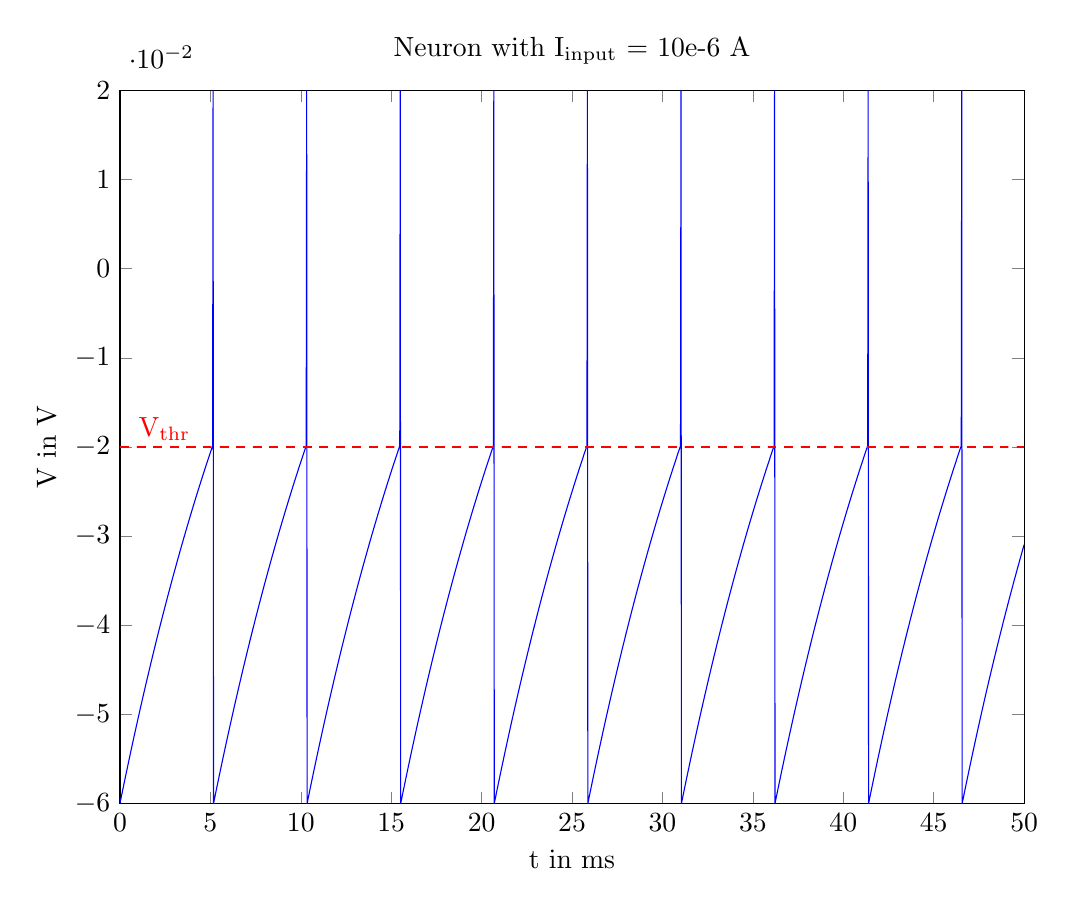
\begin{tikzpicture}

\begin{axis}[%
width=4.520833in,
height=3.565625in,
at={(0.758333in,0.48125in)},
scale only axis,
separate axis lines,
every outer x axis line/.append style={black},
every x tick label/.append style={font=\color{black}},
xmin=0,
xmax=50,
xlabel={t in ms},
every outer y axis line/.append style={black},
every y tick label/.append style={font=\color{black}},
ymin=-0.06,
ymax=0.02,
ylabel={V in V},
title={$\text{Neuron with I}_{\text{input}}\text{ = 10e-6 A}$}
]
\addplot [color=blue,solid,forget plot]
  table[row sep=crcr]{%
0	-0.06\\
0.025	-0.05975\\
0.05	-0.059500625\\
0.075	-0.0592518734375\\
0.1	-0.0590037437539062\\
0.125	-0.0587562343945215\\
0.15	-0.0585093438085352\\
0.175	-0.0582630704490138\\
0.2	-0.0580174127728913\\
0.225	-0.0577723692409591\\
0.25	-0.0575279383178567\\
0.275	-0.057284118472062\\
0.3	-0.0570409081758819\\
0.325	-0.0567983059054422\\
0.35	-0.0565563101406786\\
0.375	-0.0563149193653269\\
0.4	-0.0560741320669136\\
0.425	-0.0558339467367463\\
0.45	-0.0555943618699044\\
0.475	-0.0553553759652296\\
0.5	-0.0551169875253166\\
0.525	-0.0548791950565033\\
0.55	-0.054641997068862\\
0.575	-0.0544053920761899\\
0.6	-0.0541693785959994\\
0.625	-0.0539339551495094\\
0.65	-0.0536991202616356\\
0.675	-0.0534648724609815\\
0.7	-0.0532312102798291\\
0.725	-0.0529981322541295\\
0.75	-0.0527656369234942\\
0.775	-0.0525337228311854\\
0.8	-0.0523023885241075\\
0.825	-0.0520716325527972\\
0.85	-0.0518414534714152\\
0.875	-0.0516118498377367\\
0.9	-0.0513828202131423\\
0.925	-0.0511543631626095\\
0.95	-0.050926477254703\\
0.975	-0.0506991610615662\\
1	-0.0504724131589123\\
1.025	-0.050246232126015\\
1.05	-0.0500206165457\\
1.075	-0.0497955650043357\\
1.1	-0.0495710760918249\\
1.125	-0.0493471484015953\\
1.15	-0.0491237805305913\\
1.175	-0.0489009710792648\\
1.2	-0.0486787186515667\\
1.225	-0.0484570218549378\\
1.25	-0.0482358793003004\\
1.275	-0.0480152896020497\\
1.3	-0.0477952513780446\\
1.325	-0.0475757632495994\\
1.35	-0.0473568238414754\\
1.375	-0.0471384317818717\\
1.4	-0.0469205857024171\\
1.425	-0.046703284238161\\
1.45	-0.0464865260275656\\
1.475	-0.0462703097124967\\
1.5	-0.0460546339382155\\
1.525	-0.0458394973533699\\
1.55	-0.0456248986099865\\
1.575	-0.0454108363634615\\
1.6	-0.0451973092725529\\
1.625	-0.0449843159993715\\
1.65	-0.0447718552093731\\
1.675	-0.0445599255713496\\
1.7	-0.0443485257574213\\
1.725	-0.0441376544430277\\
1.75	-0.0439273103069201\\
1.775	-0.0437174920311528\\
1.8	-0.043508198301075\\
1.825	-0.0432994278053223\\
1.85	-0.043091179235809\\
1.875	-0.0428834512877195\\
1.9	-0.0426762426595002\\
1.925	-0.0424695520528514\\
1.95	-0.0422633781727193\\
1.975	-0.0420577197272875\\
2	-0.0418525754279693\\
2.025	-0.0416479439893993\\
2.05	-0.0414438241294258\\
2.075	-0.0412402145691023\\
2.1	-0.0410371140326795\\
2.125	-0.0408345212475978\\
2.15	-0.0406324349444788\\
2.175	-0.0404308538571176\\
2.2	-0.0402297767224748\\
2.225	-0.0400292022806687\\
2.25	-0.039829129274967\\
2.275	-0.0396295564517796\\
2.3	-0.0394304825606501\\
2.325	-0.0392319063542485\\
2.35	-0.0390338265883629\\
2.375	-0.038836242021892\\
2.4	-0.0386391514168372\\
2.425	-0.0384425535382951\\
2.45	-0.0382464471544494\\
2.475	-0.0380508310365633\\
2.5	-0.0378557039589719\\
2.525	-0.0376610646990745\\
2.55	-0.0374669120373268\\
2.575	-0.0372732447572334\\
2.6	-0.0370800616453404\\
2.625	-0.036887361491227\\
2.65	-0.0366951430874989\\
2.675	-0.0365034052297802\\
2.7	-0.0363121467167057\\
2.725	-0.036121366349914\\
2.75	-0.0359310629340392\\
2.775	-0.0357412352767041\\
2.8	-0.0355518821885123\\
2.825	-0.0353630024830411\\
2.85	-0.0351745949768335\\
2.875	-0.0349866584893914\\
2.9	-0.0347991918431679\\
2.925	-0.03461219386356\\
2.95	-0.0344256633789011\\
2.975	-0.0342395992204538\\
3	-0.0340540002224027\\
3.025	-0.0338688652218467\\
3.05	-0.033684193058792\\
3.075	-0.0334999825761451\\
3.1	-0.0333162326197047\\
3.125	-0.0331329420381554\\
3.15	-0.0329501096830601\\
3.175	-0.0327677344088524\\
3.2	-0.0325858150728303\\
3.225	-0.0324043505351482\\
3.25	-0.0322233396588103\\
3.275	-0.0320427813096633\\
3.3	-0.0318626743563891\\
3.325	-0.0316830176704982\\
3.35	-0.0315038101263219\\
3.375	-0.0313250506010061\\
3.4	-0.0311467379745036\\
3.425	-0.0309688711295673\\
3.45	-0.0307914489517434\\
3.475	-0.0306144703293641\\
3.5	-0.0304379341535406\\
3.525	-0.0302618393181568\\
3.55	-0.0300861847198614\\
3.575	-0.0299109692580617\\
3.6	-0.0297361918349166\\
3.625	-0.0295618513553293\\
3.65	-0.029387946726941\\
3.675	-0.0292144768601236\\
3.7	-0.0290414406679733\\
3.725	-0.0288688370663034\\
3.75	-0.0286966649736376\\
3.775	-0.0285249233112035\\
3.8	-0.0283536110029255\\
3.825	-0.0281827269754182\\
3.85	-0.0280122701579797\\
3.875	-0.0278422394825847\\
3.9	-0.0276726338838783\\
3.925	-0.0275034522991686\\
3.95	-0.0273346936684206\\
3.975	-0.0271663569342496\\
4	-0.026998441041914\\
4.025	-0.0268309449393092\\
4.05	-0.0266638675769609\\
4.075	-0.0264972079080185\\
4.1	-0.0263309648882485\\
4.125	-0.0261651374760278\\
4.15	-0.0259997246323378\\
4.175	-0.0258347253207569\\
4.2	-0.025670138507455\\
4.225	-0.0255059631611864\\
4.25	-0.0253421982532834\\
4.275	-0.0251788427576502\\
4.3	-0.0250158956507561\\
4.325	-0.0248533559116292\\
4.35	-0.0246912225218501\\
4.375	-0.0245294944655455\\
4.4	-0.0243681707293816\\
4.425	-0.0242072503025582\\
4.45	-0.0240467321768018\\
4.475	-0.0238866153463598\\
4.5	-0.0237268988079939\\
4.525	-0.0235675815609739\\
4.55	-0.0234086626070715\\
4.575	-0.0232501409505538\\
4.6	-0.0230920155981774\\
4.625	-0.022934285559182\\
4.65	-0.022776949845284\\
4.675	-0.0226200074706708\\
4.7	-0.0224634574519941\\
4.725	-0.0223072988083641\\
4.75	-0.0221515305613432\\
4.775	-0.0219961517349399\\
4.8	-0.0218411613556025\\
4.825	-0.0216865584522135\\
4.85	-0.021532342056083\\
4.875	-0.0213785112009428\\
4.9	-0.0212250649229404\\
4.925	-0.0210720022606331\\
4.95	-0.0209193222549815\\
4.975	-0.020767023949344\\
5	-0.0206151063894707\\
5.025	-0.020463568623497\\
5.05	-0.0203124097019382\\
5.075	-0.0201616286776834\\
5.1	-0.0200112246059892\\
5.125	-0.0198611965444742\\
5.15	0.02\\
5.175	-0.06\\
5.2	-0.05975\\
5.225	-0.059500625\\
5.25	-0.0592518734375\\
5.275	-0.0590037437539062\\
5.3	-0.0587562343945215\\
5.325	-0.0585093438085352\\
5.35	-0.0582630704490138\\
5.375	-0.0580174127728913\\
5.4	-0.0577723692409591\\
5.425	-0.0575279383178567\\
5.45	-0.057284118472062\\
5.475	-0.0570409081758819\\
5.5	-0.0567983059054422\\
5.525	-0.0565563101406786\\
5.55	-0.0563149193653269\\
5.575	-0.0560741320669136\\
5.6	-0.0558339467367463\\
5.625	-0.0555943618699044\\
5.65	-0.0553553759652296\\
5.675	-0.0551169875253166\\
5.7	-0.0548791950565033\\
5.725	-0.054641997068862\\
5.75	-0.0544053920761899\\
5.775	-0.0541693785959994\\
5.8	-0.0539339551495094\\
5.825	-0.0536991202616356\\
5.85	-0.0534648724609815\\
5.875	-0.0532312102798291\\
5.9	-0.0529981322541295\\
5.925	-0.0527656369234942\\
5.95	-0.0525337228311854\\
5.975	-0.0523023885241075\\
6	-0.0520716325527972\\
6.025	-0.0518414534714152\\
6.05	-0.0516118498377367\\
6.075	-0.0513828202131423\\
6.1	-0.0511543631626095\\
6.125	-0.050926477254703\\
6.15	-0.0506991610615662\\
6.175	-0.0504724131589123\\
6.2	-0.050246232126015\\
6.225	-0.0500206165457\\
6.25	-0.0497955650043357\\
6.275	-0.0495710760918249\\
6.3	-0.0493471484015953\\
6.325	-0.0491237805305913\\
6.35	-0.0489009710792648\\
6.375	-0.0486787186515667\\
6.4	-0.0484570218549378\\
6.425	-0.0482358793003004\\
6.45	-0.0480152896020497\\
6.475	-0.0477952513780446\\
6.5	-0.0475757632495994\\
6.525	-0.0473568238414754\\
6.55	-0.0471384317818717\\
6.575	-0.0469205857024171\\
6.6	-0.046703284238161\\
6.625	-0.0464865260275656\\
6.65	-0.0462703097124967\\
6.675	-0.0460546339382155\\
6.7	-0.0458394973533699\\
6.725	-0.0456248986099865\\
6.75	-0.0454108363634615\\
6.775	-0.0451973092725529\\
6.8	-0.0449843159993715\\
6.825	-0.0447718552093731\\
6.85	-0.0445599255713496\\
6.875	-0.0443485257574213\\
6.9	-0.0441376544430277\\
6.925	-0.0439273103069201\\
6.95	-0.0437174920311528\\
6.975	-0.043508198301075\\
7	-0.0432994278053223\\
7.025	-0.043091179235809\\
7.05	-0.0428834512877195\\
7.075	-0.0426762426595002\\
7.1	-0.0424695520528514\\
7.125	-0.0422633781727193\\
7.15	-0.0420577197272875\\
7.175	-0.0418525754279693\\
7.2	-0.0416479439893993\\
7.225	-0.0414438241294258\\
7.25	-0.0412402145691023\\
7.275	-0.0410371140326795\\
7.3	-0.0408345212475978\\
7.325	-0.0406324349444788\\
7.35	-0.0404308538571176\\
7.375	-0.0402297767224748\\
7.4	-0.0400292022806687\\
7.425	-0.039829129274967\\
7.45	-0.0396295564517796\\
7.475	-0.0394304825606501\\
7.5	-0.0392319063542485\\
7.525	-0.0390338265883629\\
7.55	-0.038836242021892\\
7.575	-0.0386391514168372\\
7.6	-0.0384425535382951\\
7.625	-0.0382464471544494\\
7.65	-0.0380508310365633\\
7.675	-0.0378557039589719\\
7.7	-0.0376610646990745\\
7.725	-0.0374669120373268\\
7.75	-0.0372732447572334\\
7.775	-0.0370800616453404\\
7.8	-0.036887361491227\\
7.825	-0.0366951430874989\\
7.85	-0.0365034052297802\\
7.875	-0.0363121467167057\\
7.9	-0.036121366349914\\
7.925	-0.0359310629340392\\
7.95	-0.0357412352767041\\
7.975	-0.0355518821885123\\
8	-0.0353630024830411\\
8.025	-0.0351745949768335\\
8.05	-0.0349866584893914\\
8.075	-0.0347991918431679\\
8.1	-0.03461219386356\\
8.125	-0.0344256633789011\\
8.15	-0.0342395992204538\\
8.175	-0.0340540002224027\\
8.2	-0.0338688652218467\\
8.225	-0.033684193058792\\
8.25	-0.0334999825761451\\
8.275	-0.0333162326197047\\
8.3	-0.0331329420381554\\
8.325	-0.0329501096830601\\
8.35	-0.0327677344088524\\
8.375	-0.0325858150728303\\
8.4	-0.0324043505351482\\
8.425	-0.0322233396588103\\
8.45	-0.0320427813096633\\
8.475	-0.0318626743563891\\
8.5	-0.0316830176704982\\
8.525	-0.0315038101263219\\
8.55	-0.0313250506010061\\
8.575	-0.0311467379745036\\
8.6	-0.0309688711295673\\
8.625	-0.0307914489517434\\
8.65	-0.0306144703293641\\
8.675	-0.0304379341535406\\
8.7	-0.0302618393181568\\
8.725	-0.0300861847198614\\
8.75	-0.0299109692580617\\
8.775	-0.0297361918349166\\
8.8	-0.0295618513553293\\
8.825	-0.029387946726941\\
8.85	-0.0292144768601236\\
8.875	-0.0290414406679733\\
8.9	-0.0288688370663034\\
8.925	-0.0286966649736376\\
8.95	-0.0285249233112035\\
8.975	-0.0283536110029255\\
9	-0.0281827269754182\\
9.025	-0.0280122701579797\\
9.05	-0.0278422394825847\\
9.075	-0.0276726338838783\\
9.1	-0.0275034522991686\\
9.125	-0.0273346936684206\\
9.15	-0.0271663569342496\\
9.175	-0.026998441041914\\
9.2	-0.0268309449393092\\
9.225	-0.0266638675769609\\
9.25	-0.0264972079080185\\
9.275	-0.0263309648882485\\
9.3	-0.0261651374760278\\
9.325	-0.0259997246323378\\
9.35	-0.0258347253207569\\
9.375	-0.025670138507455\\
9.4	-0.0255059631611864\\
9.425	-0.0253421982532834\\
9.45	-0.0251788427576502\\
9.475	-0.0250158956507561\\
9.5	-0.0248533559116292\\
9.525	-0.0246912225218501\\
9.55	-0.0245294944655455\\
9.575	-0.0243681707293816\\
9.6	-0.0242072503025582\\
9.625	-0.0240467321768018\\
9.65	-0.0238866153463598\\
9.675	-0.0237268988079939\\
9.7	-0.0235675815609739\\
9.725	-0.0234086626070715\\
9.75	-0.0232501409505538\\
9.775	-0.0230920155981774\\
9.8	-0.022934285559182\\
9.825	-0.022776949845284\\
9.85	-0.0226200074706708\\
9.875	-0.0224634574519941\\
9.9	-0.0223072988083641\\
9.925	-0.0221515305613432\\
9.95	-0.0219961517349399\\
9.975	-0.0218411613556025\\
10	-0.0216865584522135\\
10.025	-0.021532342056083\\
10.05	-0.0213785112009428\\
10.075	-0.0212250649229404\\
10.1	-0.0210720022606331\\
10.125	-0.0209193222549815\\
10.15	-0.020767023949344\\
10.175	-0.0206151063894707\\
10.2	-0.020463568623497\\
10.225	-0.0203124097019382\\
10.25	-0.0201616286776834\\
10.275	-0.0200112246059892\\
10.3	-0.0198611965444742\\
10.325	0.02\\
10.35	-0.06\\
10.375	-0.05975\\
10.4	-0.059500625\\
10.425	-0.0592518734375\\
10.45	-0.0590037437539062\\
10.475	-0.0587562343945215\\
10.5	-0.0585093438085352\\
10.525	-0.0582630704490138\\
10.55	-0.0580174127728913\\
10.575	-0.0577723692409591\\
10.6	-0.0575279383178567\\
10.625	-0.057284118472062\\
10.65	-0.0570409081758819\\
10.675	-0.0567983059054422\\
10.7	-0.0565563101406786\\
10.725	-0.0563149193653269\\
10.75	-0.0560741320669136\\
10.775	-0.0558339467367463\\
10.8	-0.0555943618699044\\
10.825	-0.0553553759652296\\
10.85	-0.0551169875253166\\
10.875	-0.0548791950565033\\
10.9	-0.054641997068862\\
10.925	-0.0544053920761899\\
10.95	-0.0541693785959994\\
10.975	-0.0539339551495094\\
11	-0.0536991202616356\\
11.025	-0.0534648724609815\\
11.05	-0.0532312102798291\\
11.075	-0.0529981322541295\\
11.1	-0.0527656369234942\\
11.125	-0.0525337228311854\\
11.15	-0.0523023885241075\\
11.175	-0.0520716325527972\\
11.2	-0.0518414534714152\\
11.225	-0.0516118498377367\\
11.25	-0.0513828202131423\\
11.275	-0.0511543631626095\\
11.3	-0.050926477254703\\
11.325	-0.0506991610615662\\
11.35	-0.0504724131589123\\
11.375	-0.050246232126015\\
11.4	-0.0500206165457\\
11.425	-0.0497955650043357\\
11.45	-0.0495710760918249\\
11.475	-0.0493471484015953\\
11.5	-0.0491237805305913\\
11.525	-0.0489009710792648\\
11.55	-0.0486787186515667\\
11.575	-0.0484570218549378\\
11.6	-0.0482358793003004\\
11.625	-0.0480152896020497\\
11.65	-0.0477952513780446\\
11.675	-0.0475757632495994\\
11.7	-0.0473568238414754\\
11.725	-0.0471384317818717\\
11.75	-0.0469205857024171\\
11.775	-0.046703284238161\\
11.8	-0.0464865260275656\\
11.825	-0.0462703097124967\\
11.85	-0.0460546339382155\\
11.875	-0.0458394973533699\\
11.9	-0.0456248986099865\\
11.925	-0.0454108363634615\\
11.95	-0.0451973092725529\\
11.975	-0.0449843159993715\\
12	-0.0447718552093731\\
12.025	-0.0445599255713496\\
12.05	-0.0443485257574213\\
12.075	-0.0441376544430277\\
12.1	-0.0439273103069201\\
12.125	-0.0437174920311528\\
12.15	-0.043508198301075\\
12.175	-0.0432994278053223\\
12.2	-0.043091179235809\\
12.225	-0.0428834512877195\\
12.25	-0.0426762426595002\\
12.275	-0.0424695520528514\\
12.3	-0.0422633781727193\\
12.325	-0.0420577197272875\\
12.35	-0.0418525754279693\\
12.375	-0.0416479439893993\\
12.4	-0.0414438241294258\\
12.425	-0.0412402145691023\\
12.45	-0.0410371140326795\\
12.475	-0.0408345212475978\\
12.5	-0.0406324349444788\\
12.525	-0.0404308538571176\\
12.55	-0.0402297767224748\\
12.575	-0.0400292022806687\\
12.6	-0.039829129274967\\
12.625	-0.0396295564517796\\
12.65	-0.0394304825606501\\
12.675	-0.0392319063542485\\
12.7	-0.0390338265883629\\
12.725	-0.038836242021892\\
12.75	-0.0386391514168372\\
12.775	-0.0384425535382951\\
12.8	-0.0382464471544494\\
12.825	-0.0380508310365633\\
12.85	-0.0378557039589719\\
12.875	-0.0376610646990745\\
12.9	-0.0374669120373268\\
12.925	-0.0372732447572334\\
12.95	-0.0370800616453404\\
12.975	-0.036887361491227\\
13	-0.0366951430874989\\
13.025	-0.0365034052297802\\
13.05	-0.0363121467167057\\
13.075	-0.036121366349914\\
13.1	-0.0359310629340392\\
13.125	-0.0357412352767041\\
13.15	-0.0355518821885123\\
13.175	-0.0353630024830411\\
13.2	-0.0351745949768335\\
13.225	-0.0349866584893914\\
13.25	-0.0347991918431679\\
13.275	-0.03461219386356\\
13.3	-0.0344256633789011\\
13.325	-0.0342395992204538\\
13.35	-0.0340540002224027\\
13.375	-0.0338688652218467\\
13.4	-0.033684193058792\\
13.425	-0.0334999825761451\\
13.45	-0.0333162326197047\\
13.475	-0.0331329420381554\\
13.5	-0.0329501096830601\\
13.525	-0.0327677344088524\\
13.55	-0.0325858150728303\\
13.575	-0.0324043505351482\\
13.6	-0.0322233396588103\\
13.625	-0.0320427813096633\\
13.65	-0.0318626743563891\\
13.675	-0.0316830176704982\\
13.7	-0.0315038101263219\\
13.725	-0.0313250506010061\\
13.75	-0.0311467379745036\\
13.775	-0.0309688711295673\\
13.8	-0.0307914489517434\\
13.825	-0.0306144703293641\\
13.85	-0.0304379341535406\\
13.875	-0.0302618393181568\\
13.9	-0.0300861847198614\\
13.925	-0.0299109692580617\\
13.95	-0.0297361918349166\\
13.975	-0.0295618513553293\\
14	-0.029387946726941\\
14.025	-0.0292144768601236\\
14.05	-0.0290414406679733\\
14.075	-0.0288688370663034\\
14.1	-0.0286966649736376\\
14.125	-0.0285249233112035\\
14.15	-0.0283536110029255\\
14.175	-0.0281827269754182\\
14.2	-0.0280122701579797\\
14.225	-0.0278422394825847\\
14.25	-0.0276726338838783\\
14.275	-0.0275034522991686\\
14.3	-0.0273346936684206\\
14.325	-0.0271663569342496\\
14.35	-0.026998441041914\\
14.375	-0.0268309449393092\\
14.4	-0.0266638675769609\\
14.425	-0.0264972079080185\\
14.45	-0.0263309648882485\\
14.475	-0.0261651374760278\\
14.5	-0.0259997246323378\\
14.525	-0.0258347253207569\\
14.55	-0.025670138507455\\
14.575	-0.0255059631611864\\
14.6	-0.0253421982532834\\
14.625	-0.0251788427576502\\
14.65	-0.0250158956507561\\
14.675	-0.0248533559116292\\
14.7	-0.0246912225218501\\
14.725	-0.0245294944655455\\
14.75	-0.0243681707293816\\
14.775	-0.0242072503025582\\
14.8	-0.0240467321768018\\
14.825	-0.0238866153463598\\
14.85	-0.0237268988079939\\
14.875	-0.0235675815609739\\
14.9	-0.0234086626070715\\
14.925	-0.0232501409505538\\
14.95	-0.0230920155981774\\
14.975	-0.022934285559182\\
15	-0.022776949845284\\
15.025	-0.0226200074706708\\
15.05	-0.0224634574519941\\
15.075	-0.0223072988083641\\
15.1	-0.0221515305613432\\
15.125	-0.0219961517349399\\
15.15	-0.0218411613556025\\
15.175	-0.0216865584522135\\
15.2	-0.021532342056083\\
15.225	-0.0213785112009428\\
15.25	-0.0212250649229404\\
15.275	-0.0210720022606331\\
15.3	-0.0209193222549815\\
15.325	-0.020767023949344\\
15.35	-0.0206151063894707\\
15.375	-0.020463568623497\\
15.4	-0.0203124097019382\\
15.425	-0.0201616286776834\\
15.45	-0.0200112246059892\\
15.475	-0.0198611965444742\\
15.5	0.02\\
15.525	-0.06\\
15.55	-0.05975\\
15.575	-0.059500625\\
15.6	-0.0592518734375\\
15.625	-0.0590037437539062\\
15.65	-0.0587562343945215\\
15.675	-0.0585093438085352\\
15.7	-0.0582630704490138\\
15.725	-0.0580174127728913\\
15.75	-0.0577723692409591\\
15.775	-0.0575279383178567\\
15.8	-0.057284118472062\\
15.825	-0.0570409081758819\\
15.85	-0.0567983059054422\\
15.875	-0.0565563101406786\\
15.9	-0.0563149193653269\\
15.925	-0.0560741320669136\\
15.95	-0.0558339467367463\\
15.975	-0.0555943618699044\\
16	-0.0553553759652296\\
16.025	-0.0551169875253166\\
16.05	-0.0548791950565033\\
16.075	-0.054641997068862\\
16.1	-0.0544053920761899\\
16.125	-0.0541693785959994\\
16.15	-0.0539339551495094\\
16.175	-0.0536991202616356\\
16.2	-0.0534648724609815\\
16.225	-0.0532312102798291\\
16.25	-0.0529981322541295\\
16.275	-0.0527656369234942\\
16.3	-0.0525337228311854\\
16.325	-0.0523023885241075\\
16.35	-0.0520716325527972\\
16.375	-0.0518414534714152\\
16.4	-0.0516118498377367\\
16.425	-0.0513828202131423\\
16.45	-0.0511543631626095\\
16.475	-0.050926477254703\\
16.5	-0.0506991610615662\\
16.525	-0.0504724131589123\\
16.55	-0.050246232126015\\
16.575	-0.0500206165457\\
16.6	-0.0497955650043357\\
16.625	-0.0495710760918249\\
16.65	-0.0493471484015953\\
16.675	-0.0491237805305913\\
16.7	-0.0489009710792648\\
16.725	-0.0486787186515667\\
16.75	-0.0484570218549378\\
16.775	-0.0482358793003004\\
16.8	-0.0480152896020497\\
16.825	-0.0477952513780446\\
16.85	-0.0475757632495994\\
16.875	-0.0473568238414754\\
16.9	-0.0471384317818717\\
16.925	-0.0469205857024171\\
16.95	-0.046703284238161\\
16.975	-0.0464865260275656\\
17	-0.0462703097124967\\
17.025	-0.0460546339382155\\
17.05	-0.0458394973533699\\
17.075	-0.0456248986099865\\
17.1	-0.0454108363634615\\
17.125	-0.0451973092725529\\
17.15	-0.0449843159993715\\
17.175	-0.0447718552093731\\
17.2	-0.0445599255713496\\
17.225	-0.0443485257574213\\
17.25	-0.0441376544430277\\
17.275	-0.0439273103069201\\
17.3	-0.0437174920311528\\
17.325	-0.043508198301075\\
17.35	-0.0432994278053223\\
17.375	-0.043091179235809\\
17.4	-0.0428834512877195\\
17.425	-0.0426762426595002\\
17.45	-0.0424695520528514\\
17.475	-0.0422633781727193\\
17.5	-0.0420577197272875\\
17.525	-0.0418525754279693\\
17.55	-0.0416479439893993\\
17.575	-0.0414438241294258\\
17.6	-0.0412402145691023\\
17.625	-0.0410371140326795\\
17.65	-0.0408345212475978\\
17.675	-0.0406324349444788\\
17.7	-0.0404308538571176\\
17.725	-0.0402297767224748\\
17.75	-0.0400292022806687\\
17.775	-0.039829129274967\\
17.8	-0.0396295564517796\\
17.825	-0.0394304825606501\\
17.85	-0.0392319063542485\\
17.875	-0.0390338265883629\\
17.9	-0.038836242021892\\
17.925	-0.0386391514168372\\
17.95	-0.0384425535382951\\
17.975	-0.0382464471544494\\
18	-0.0380508310365633\\
18.025	-0.0378557039589719\\
18.05	-0.0376610646990745\\
18.075	-0.0374669120373268\\
18.1	-0.0372732447572334\\
18.125	-0.0370800616453404\\
18.15	-0.036887361491227\\
18.175	-0.0366951430874989\\
18.2	-0.0365034052297802\\
18.225	-0.0363121467167057\\
18.25	-0.036121366349914\\
18.275	-0.0359310629340392\\
18.3	-0.0357412352767041\\
18.325	-0.0355518821885123\\
18.35	-0.0353630024830411\\
18.375	-0.0351745949768335\\
18.4	-0.0349866584893914\\
18.425	-0.0347991918431679\\
18.45	-0.03461219386356\\
18.475	-0.0344256633789011\\
18.5	-0.0342395992204538\\
18.525	-0.0340540002224027\\
18.55	-0.0338688652218467\\
18.575	-0.033684193058792\\
18.6	-0.0334999825761451\\
18.625	-0.0333162326197047\\
18.65	-0.0331329420381554\\
18.675	-0.0329501096830601\\
18.7	-0.0327677344088524\\
18.725	-0.0325858150728303\\
18.75	-0.0324043505351482\\
18.775	-0.0322233396588103\\
18.8	-0.0320427813096633\\
18.825	-0.0318626743563891\\
18.85	-0.0316830176704982\\
18.875	-0.0315038101263219\\
18.9	-0.0313250506010061\\
18.925	-0.0311467379745036\\
18.95	-0.0309688711295673\\
18.975	-0.0307914489517434\\
19	-0.0306144703293641\\
19.025	-0.0304379341535406\\
19.05	-0.0302618393181568\\
19.075	-0.0300861847198614\\
19.1	-0.0299109692580617\\
19.125	-0.0297361918349166\\
19.15	-0.0295618513553293\\
19.175	-0.029387946726941\\
19.2	-0.0292144768601236\\
19.225	-0.0290414406679733\\
19.25	-0.0288688370663034\\
19.275	-0.0286966649736376\\
19.3	-0.0285249233112035\\
19.325	-0.0283536110029255\\
19.35	-0.0281827269754182\\
19.375	-0.0280122701579797\\
19.4	-0.0278422394825847\\
19.425	-0.0276726338838783\\
19.45	-0.0275034522991686\\
19.475	-0.0273346936684206\\
19.5	-0.0271663569342496\\
19.525	-0.026998441041914\\
19.55	-0.0268309449393092\\
19.575	-0.0266638675769609\\
19.6	-0.0264972079080185\\
19.625	-0.0263309648882485\\
19.65	-0.0261651374760278\\
19.675	-0.0259997246323378\\
19.7	-0.0258347253207569\\
19.725	-0.025670138507455\\
19.75	-0.0255059631611864\\
19.775	-0.0253421982532834\\
19.8	-0.0251788427576502\\
19.825	-0.0250158956507561\\
19.85	-0.0248533559116292\\
19.875	-0.0246912225218501\\
19.9	-0.0245294944655455\\
19.925	-0.0243681707293816\\
19.95	-0.0242072503025582\\
19.975	-0.0240467321768018\\
20	-0.0238866153463598\\
20.025	-0.0237268988079939\\
20.05	-0.0235675815609739\\
20.075	-0.0234086626070715\\
20.1	-0.0232501409505538\\
20.125	-0.0230920155981774\\
20.15	-0.022934285559182\\
20.175	-0.022776949845284\\
20.2	-0.0226200074706708\\
20.225	-0.0224634574519941\\
20.25	-0.0223072988083641\\
20.275	-0.0221515305613432\\
20.3	-0.0219961517349399\\
20.325	-0.0218411613556025\\
20.35	-0.0216865584522135\\
20.375	-0.021532342056083\\
20.4	-0.0213785112009428\\
20.425	-0.0212250649229404\\
20.45	-0.0210720022606331\\
20.475	-0.0209193222549815\\
20.5	-0.020767023949344\\
20.525	-0.0206151063894707\\
20.55	-0.020463568623497\\
20.575	-0.0203124097019382\\
20.6	-0.0201616286776834\\
20.625	-0.0200112246059892\\
20.65	-0.0198611965444742\\
20.675	0.02\\
20.7	-0.06\\
20.725	-0.05975\\
20.75	-0.059500625\\
20.775	-0.0592518734375\\
20.8	-0.0590037437539062\\
20.825	-0.0587562343945215\\
20.85	-0.0585093438085352\\
20.875	-0.0582630704490138\\
20.9	-0.0580174127728913\\
20.925	-0.0577723692409591\\
20.95	-0.0575279383178567\\
20.975	-0.057284118472062\\
21	-0.0570409081758819\\
21.025	-0.0567983059054422\\
21.05	-0.0565563101406786\\
21.075	-0.0563149193653269\\
21.1	-0.0560741320669136\\
21.125	-0.0558339467367463\\
21.15	-0.0555943618699044\\
21.175	-0.0553553759652296\\
21.2	-0.0551169875253166\\
21.225	-0.0548791950565033\\
21.25	-0.054641997068862\\
21.275	-0.0544053920761899\\
21.3	-0.0541693785959994\\
21.325	-0.0539339551495094\\
21.35	-0.0536991202616356\\
21.375	-0.0534648724609815\\
21.4	-0.0532312102798291\\
21.425	-0.0529981322541295\\
21.45	-0.0527656369234942\\
21.475	-0.0525337228311854\\
21.5	-0.0523023885241075\\
21.525	-0.0520716325527972\\
21.55	-0.0518414534714152\\
21.575	-0.0516118498377367\\
21.6	-0.0513828202131423\\
21.625	-0.0511543631626095\\
21.65	-0.050926477254703\\
21.675	-0.0506991610615662\\
21.7	-0.0504724131589123\\
21.725	-0.050246232126015\\
21.75	-0.0500206165457\\
21.775	-0.0497955650043357\\
21.8	-0.0495710760918249\\
21.825	-0.0493471484015953\\
21.85	-0.0491237805305913\\
21.875	-0.0489009710792648\\
21.9	-0.0486787186515667\\
21.925	-0.0484570218549378\\
21.95	-0.0482358793003004\\
21.975	-0.0480152896020497\\
22	-0.0477952513780446\\
22.025	-0.0475757632495994\\
22.05	-0.0473568238414754\\
22.075	-0.0471384317818717\\
22.1	-0.0469205857024171\\
22.125	-0.046703284238161\\
22.15	-0.0464865260275656\\
22.175	-0.0462703097124967\\
22.2	-0.0460546339382155\\
22.225	-0.0458394973533699\\
22.25	-0.0456248986099865\\
22.275	-0.0454108363634615\\
22.3	-0.0451973092725529\\
22.325	-0.0449843159993715\\
22.35	-0.0447718552093731\\
22.375	-0.0445599255713496\\
22.4	-0.0443485257574213\\
22.425	-0.0441376544430277\\
22.45	-0.0439273103069201\\
22.475	-0.0437174920311528\\
22.5	-0.043508198301075\\
22.525	-0.0432994278053223\\
22.55	-0.043091179235809\\
22.575	-0.0428834512877195\\
22.6	-0.0426762426595002\\
22.625	-0.0424695520528514\\
22.65	-0.0422633781727193\\
22.675	-0.0420577197272875\\
22.7	-0.0418525754279693\\
22.725	-0.0416479439893993\\
22.75	-0.0414438241294258\\
22.775	-0.0412402145691023\\
22.8	-0.0410371140326795\\
22.825	-0.0408345212475978\\
22.85	-0.0406324349444788\\
22.875	-0.0404308538571176\\
22.9	-0.0402297767224748\\
22.925	-0.0400292022806687\\
22.95	-0.039829129274967\\
22.975	-0.0396295564517796\\
23	-0.0394304825606501\\
23.025	-0.0392319063542485\\
23.05	-0.0390338265883629\\
23.075	-0.038836242021892\\
23.1	-0.0386391514168372\\
23.125	-0.0384425535382951\\
23.15	-0.0382464471544494\\
23.175	-0.0380508310365633\\
23.2	-0.0378557039589719\\
23.225	-0.0376610646990745\\
23.25	-0.0374669120373268\\
23.275	-0.0372732447572334\\
23.3	-0.0370800616453404\\
23.325	-0.036887361491227\\
23.35	-0.0366951430874989\\
23.375	-0.0365034052297802\\
23.4	-0.0363121467167057\\
23.425	-0.036121366349914\\
23.45	-0.0359310629340392\\
23.475	-0.0357412352767041\\
23.5	-0.0355518821885123\\
23.525	-0.0353630024830411\\
23.55	-0.0351745949768335\\
23.575	-0.0349866584893914\\
23.6	-0.0347991918431679\\
23.625	-0.03461219386356\\
23.65	-0.0344256633789011\\
23.675	-0.0342395992204538\\
23.7	-0.0340540002224027\\
23.725	-0.0338688652218467\\
23.75	-0.033684193058792\\
23.775	-0.0334999825761451\\
23.8	-0.0333162326197047\\
23.825	-0.0331329420381554\\
23.85	-0.0329501096830601\\
23.875	-0.0327677344088524\\
23.9	-0.0325858150728303\\
23.925	-0.0324043505351482\\
23.95	-0.0322233396588103\\
23.975	-0.0320427813096633\\
24	-0.0318626743563891\\
24.025	-0.0316830176704982\\
24.05	-0.0315038101263219\\
24.075	-0.0313250506010061\\
24.1	-0.0311467379745036\\
24.125	-0.0309688711295673\\
24.15	-0.0307914489517434\\
24.175	-0.0306144703293641\\
24.2	-0.0304379341535406\\
24.225	-0.0302618393181568\\
24.25	-0.0300861847198614\\
24.275	-0.0299109692580617\\
24.3	-0.0297361918349166\\
24.325	-0.0295618513553293\\
24.35	-0.029387946726941\\
24.375	-0.0292144768601236\\
24.4	-0.0290414406679733\\
24.425	-0.0288688370663034\\
24.45	-0.0286966649736376\\
24.475	-0.0285249233112035\\
24.5	-0.0283536110029255\\
24.525	-0.0281827269754182\\
24.55	-0.0280122701579797\\
24.575	-0.0278422394825847\\
24.6	-0.0276726338838783\\
24.625	-0.0275034522991686\\
24.65	-0.0273346936684206\\
24.675	-0.0271663569342496\\
24.7	-0.026998441041914\\
24.725	-0.0268309449393092\\
24.75	-0.0266638675769609\\
24.775	-0.0264972079080185\\
24.8	-0.0263309648882485\\
24.825	-0.0261651374760278\\
24.85	-0.0259997246323378\\
24.875	-0.0258347253207569\\
24.9	-0.025670138507455\\
24.925	-0.0255059631611864\\
24.95	-0.0253421982532834\\
24.975	-0.0251788427576502\\
25	-0.0250158956507561\\
25.025	-0.0248533559116292\\
25.05	-0.0246912225218501\\
25.075	-0.0245294944655455\\
25.1	-0.0243681707293816\\
25.125	-0.0242072503025582\\
25.15	-0.0240467321768018\\
25.175	-0.0238866153463598\\
25.2	-0.0237268988079939\\
25.225	-0.0235675815609739\\
25.25	-0.0234086626070715\\
25.275	-0.0232501409505538\\
25.3	-0.0230920155981774\\
25.325	-0.022934285559182\\
25.35	-0.022776949845284\\
25.375	-0.0226200074706708\\
25.4	-0.0224634574519941\\
25.425	-0.0223072988083641\\
25.45	-0.0221515305613432\\
25.475	-0.0219961517349399\\
25.5	-0.0218411613556025\\
25.525	-0.0216865584522135\\
25.55	-0.021532342056083\\
25.575	-0.0213785112009428\\
25.6	-0.0212250649229404\\
25.625	-0.0210720022606331\\
25.65	-0.0209193222549815\\
25.675	-0.020767023949344\\
25.7	-0.0206151063894707\\
25.725	-0.020463568623497\\
25.75	-0.0203124097019382\\
25.775	-0.0201616286776834\\
25.8	-0.0200112246059892\\
25.825	-0.0198611965444742\\
25.85	0.02\\
25.875	-0.06\\
25.9	-0.05975\\
25.925	-0.059500625\\
25.95	-0.0592518734375\\
25.975	-0.0590037437539062\\
26	-0.0587562343945215\\
26.025	-0.0585093438085352\\
26.05	-0.0582630704490138\\
26.075	-0.0580174127728913\\
26.1	-0.0577723692409591\\
26.125	-0.0575279383178567\\
26.15	-0.057284118472062\\
26.175	-0.0570409081758819\\
26.2	-0.0567983059054422\\
26.225	-0.0565563101406786\\
26.25	-0.0563149193653269\\
26.275	-0.0560741320669136\\
26.3	-0.0558339467367463\\
26.325	-0.0555943618699044\\
26.35	-0.0553553759652296\\
26.375	-0.0551169875253166\\
26.4	-0.0548791950565033\\
26.425	-0.054641997068862\\
26.45	-0.0544053920761899\\
26.475	-0.0541693785959994\\
26.5	-0.0539339551495094\\
26.525	-0.0536991202616356\\
26.55	-0.0534648724609815\\
26.575	-0.0532312102798291\\
26.6	-0.0529981322541295\\
26.625	-0.0527656369234942\\
26.65	-0.0525337228311854\\
26.675	-0.0523023885241075\\
26.7	-0.0520716325527972\\
26.725	-0.0518414534714152\\
26.75	-0.0516118498377367\\
26.775	-0.0513828202131423\\
26.8	-0.0511543631626095\\
26.825	-0.050926477254703\\
26.85	-0.0506991610615662\\
26.875	-0.0504724131589123\\
26.9	-0.050246232126015\\
26.925	-0.0500206165457\\
26.95	-0.0497955650043357\\
26.975	-0.0495710760918249\\
27	-0.0493471484015953\\
27.025	-0.0491237805305913\\
27.05	-0.0489009710792648\\
27.075	-0.0486787186515667\\
27.1	-0.0484570218549378\\
27.125	-0.0482358793003004\\
27.15	-0.0480152896020497\\
27.175	-0.0477952513780446\\
27.2	-0.0475757632495994\\
27.225	-0.0473568238414754\\
27.25	-0.0471384317818717\\
27.275	-0.0469205857024171\\
27.3	-0.046703284238161\\
27.325	-0.0464865260275656\\
27.35	-0.0462703097124967\\
27.375	-0.0460546339382155\\
27.4	-0.0458394973533699\\
27.425	-0.0456248986099865\\
27.45	-0.0454108363634615\\
27.475	-0.0451973092725529\\
27.5	-0.0449843159993715\\
27.525	-0.0447718552093731\\
27.55	-0.0445599255713496\\
27.575	-0.0443485257574213\\
27.6	-0.0441376544430277\\
27.625	-0.0439273103069201\\
27.65	-0.0437174920311528\\
27.675	-0.043508198301075\\
27.7	-0.0432994278053223\\
27.725	-0.043091179235809\\
27.75	-0.0428834512877195\\
27.775	-0.0426762426595002\\
27.8	-0.0424695520528514\\
27.825	-0.0422633781727193\\
27.85	-0.0420577197272875\\
27.875	-0.0418525754279693\\
27.9	-0.0416479439893993\\
27.925	-0.0414438241294258\\
27.95	-0.0412402145691023\\
27.975	-0.0410371140326795\\
28	-0.0408345212475978\\
28.025	-0.0406324349444788\\
28.05	-0.0404308538571176\\
28.075	-0.0402297767224748\\
28.1	-0.0400292022806687\\
28.125	-0.039829129274967\\
28.15	-0.0396295564517796\\
28.175	-0.0394304825606501\\
28.2	-0.0392319063542485\\
28.225	-0.0390338265883629\\
28.25	-0.038836242021892\\
28.275	-0.0386391514168372\\
28.3	-0.0384425535382951\\
28.325	-0.0382464471544494\\
28.35	-0.0380508310365633\\
28.375	-0.0378557039589719\\
28.4	-0.0376610646990745\\
28.425	-0.0374669120373268\\
28.45	-0.0372732447572334\\
28.475	-0.0370800616453404\\
28.5	-0.036887361491227\\
28.525	-0.0366951430874989\\
28.55	-0.0365034052297802\\
28.575	-0.0363121467167057\\
28.6	-0.036121366349914\\
28.625	-0.0359310629340392\\
28.65	-0.0357412352767041\\
28.675	-0.0355518821885123\\
28.7	-0.0353630024830411\\
28.725	-0.0351745949768335\\
28.75	-0.0349866584893914\\
28.775	-0.0347991918431679\\
28.8	-0.03461219386356\\
28.825	-0.0344256633789011\\
28.85	-0.0342395992204538\\
28.875	-0.0340540002224027\\
28.9	-0.0338688652218467\\
28.925	-0.033684193058792\\
28.95	-0.0334999825761451\\
28.975	-0.0333162326197047\\
29	-0.0331329420381554\\
29.025	-0.0329501096830601\\
29.05	-0.0327677344088524\\
29.075	-0.0325858150728303\\
29.1	-0.0324043505351482\\
29.125	-0.0322233396588103\\
29.15	-0.0320427813096633\\
29.175	-0.0318626743563891\\
29.2	-0.0316830176704982\\
29.225	-0.0315038101263219\\
29.25	-0.0313250506010061\\
29.275	-0.0311467379745036\\
29.3	-0.0309688711295673\\
29.325	-0.0307914489517434\\
29.35	-0.0306144703293641\\
29.375	-0.0304379341535406\\
29.4	-0.0302618393181568\\
29.425	-0.0300861847198614\\
29.45	-0.0299109692580617\\
29.475	-0.0297361918349166\\
29.5	-0.0295618513553293\\
29.525	-0.029387946726941\\
29.55	-0.0292144768601236\\
29.575	-0.0290414406679733\\
29.6	-0.0288688370663034\\
29.625	-0.0286966649736376\\
29.65	-0.0285249233112035\\
29.675	-0.0283536110029255\\
29.7	-0.0281827269754182\\
29.725	-0.0280122701579797\\
29.75	-0.0278422394825847\\
29.775	-0.0276726338838783\\
29.8	-0.0275034522991686\\
29.825	-0.0273346936684206\\
29.85	-0.0271663569342496\\
29.875	-0.026998441041914\\
29.9	-0.0268309449393092\\
29.925	-0.0266638675769609\\
29.95	-0.0264972079080185\\
29.975	-0.0263309648882485\\
30	-0.0261651374760278\\
30.025	-0.0259997246323378\\
30.05	-0.0258347253207569\\
30.075	-0.025670138507455\\
30.1	-0.0255059631611864\\
30.125	-0.0253421982532834\\
30.15	-0.0251788427576502\\
30.175	-0.0250158956507561\\
30.2	-0.0248533559116292\\
30.225	-0.0246912225218501\\
30.25	-0.0245294944655455\\
30.275	-0.0243681707293816\\
30.3	-0.0242072503025582\\
30.325	-0.0240467321768018\\
30.35	-0.0238866153463598\\
30.375	-0.0237268988079939\\
30.4	-0.0235675815609739\\
30.425	-0.0234086626070715\\
30.45	-0.0232501409505538\\
30.475	-0.0230920155981774\\
30.5	-0.022934285559182\\
30.525	-0.022776949845284\\
30.55	-0.0226200074706708\\
30.575	-0.0224634574519941\\
30.6	-0.0223072988083641\\
30.625	-0.0221515305613432\\
30.65	-0.0219961517349399\\
30.675	-0.0218411613556025\\
30.7	-0.0216865584522135\\
30.725	-0.021532342056083\\
30.75	-0.0213785112009428\\
30.775	-0.0212250649229404\\
30.8	-0.0210720022606331\\
30.825	-0.0209193222549815\\
30.85	-0.020767023949344\\
30.875	-0.0206151063894707\\
30.9	-0.020463568623497\\
30.925	-0.0203124097019382\\
30.95	-0.0201616286776834\\
30.975	-0.0200112246059892\\
31	-0.0198611965444742\\
31.025	0.02\\
31.05	-0.06\\
31.075	-0.05975\\
31.1	-0.059500625\\
31.125	-0.0592518734375\\
31.15	-0.0590037437539062\\
31.175	-0.0587562343945215\\
31.2	-0.0585093438085352\\
31.225	-0.0582630704490138\\
31.25	-0.0580174127728913\\
31.275	-0.0577723692409591\\
31.3	-0.0575279383178567\\
31.325	-0.057284118472062\\
31.35	-0.0570409081758819\\
31.375	-0.0567983059054422\\
31.4	-0.0565563101406786\\
31.425	-0.0563149193653269\\
31.45	-0.0560741320669136\\
31.475	-0.0558339467367463\\
31.5	-0.0555943618699044\\
31.525	-0.0553553759652296\\
31.55	-0.0551169875253166\\
31.575	-0.0548791950565033\\
31.6	-0.054641997068862\\
31.625	-0.0544053920761899\\
31.65	-0.0541693785959994\\
31.675	-0.0539339551495094\\
31.7	-0.0536991202616356\\
31.725	-0.0534648724609815\\
31.75	-0.0532312102798291\\
31.775	-0.0529981322541295\\
31.8	-0.0527656369234942\\
31.825	-0.0525337228311854\\
31.85	-0.0523023885241075\\
31.875	-0.0520716325527972\\
31.9	-0.0518414534714152\\
31.925	-0.0516118498377367\\
31.95	-0.0513828202131423\\
31.975	-0.0511543631626095\\
32	-0.050926477254703\\
32.025	-0.0506991610615662\\
32.05	-0.0504724131589123\\
32.075	-0.050246232126015\\
32.1	-0.0500206165457\\
32.125	-0.0497955650043357\\
32.15	-0.0495710760918249\\
32.175	-0.0493471484015953\\
32.2	-0.0491237805305913\\
32.225	-0.0489009710792648\\
32.25	-0.0486787186515667\\
32.275	-0.0484570218549378\\
32.3	-0.0482358793003004\\
32.325	-0.0480152896020497\\
32.35	-0.0477952513780446\\
32.375	-0.0475757632495994\\
32.4	-0.0473568238414754\\
32.425	-0.0471384317818717\\
32.45	-0.0469205857024171\\
32.475	-0.046703284238161\\
32.5	-0.0464865260275656\\
32.525	-0.0462703097124967\\
32.55	-0.0460546339382155\\
32.575	-0.0458394973533699\\
32.6	-0.0456248986099865\\
32.625	-0.0454108363634615\\
32.65	-0.0451973092725529\\
32.675	-0.0449843159993715\\
32.7	-0.0447718552093731\\
32.725	-0.0445599255713496\\
32.75	-0.0443485257574213\\
32.775	-0.0441376544430277\\
32.8	-0.0439273103069201\\
32.825	-0.0437174920311528\\
32.85	-0.043508198301075\\
32.875	-0.0432994278053223\\
32.9	-0.043091179235809\\
32.925	-0.0428834512877195\\
32.95	-0.0426762426595002\\
32.975	-0.0424695520528514\\
33	-0.0422633781727193\\
33.025	-0.0420577197272875\\
33.05	-0.0418525754279693\\
33.075	-0.0416479439893993\\
33.1	-0.0414438241294258\\
33.125	-0.0412402145691023\\
33.15	-0.0410371140326795\\
33.175	-0.0408345212475978\\
33.2	-0.0406324349444788\\
33.225	-0.0404308538571176\\
33.25	-0.0402297767224748\\
33.275	-0.0400292022806687\\
33.3	-0.039829129274967\\
33.325	-0.0396295564517796\\
33.35	-0.0394304825606501\\
33.375	-0.0392319063542485\\
33.4	-0.0390338265883629\\
33.425	-0.038836242021892\\
33.45	-0.0386391514168372\\
33.475	-0.0384425535382951\\
33.5	-0.0382464471544494\\
33.525	-0.0380508310365633\\
33.55	-0.0378557039589719\\
33.575	-0.0376610646990745\\
33.6	-0.0374669120373268\\
33.625	-0.0372732447572334\\
33.65	-0.0370800616453404\\
33.675	-0.036887361491227\\
33.7	-0.0366951430874989\\
33.725	-0.0365034052297802\\
33.75	-0.0363121467167057\\
33.775	-0.036121366349914\\
33.8	-0.0359310629340392\\
33.825	-0.0357412352767041\\
33.85	-0.0355518821885123\\
33.875	-0.0353630024830411\\
33.9	-0.0351745949768335\\
33.925	-0.0349866584893914\\
33.95	-0.0347991918431679\\
33.975	-0.03461219386356\\
34	-0.0344256633789011\\
34.025	-0.0342395992204538\\
34.05	-0.0340540002224027\\
34.075	-0.0338688652218467\\
34.1	-0.033684193058792\\
34.125	-0.0334999825761451\\
34.15	-0.0333162326197047\\
34.175	-0.0331329420381554\\
34.2	-0.0329501096830601\\
34.225	-0.0327677344088524\\
34.25	-0.0325858150728303\\
34.275	-0.0324043505351482\\
34.3	-0.0322233396588103\\
34.325	-0.0320427813096633\\
34.35	-0.0318626743563891\\
34.375	-0.0316830176704982\\
34.4	-0.0315038101263219\\
34.425	-0.0313250506010061\\
34.45	-0.0311467379745036\\
34.475	-0.0309688711295673\\
34.5	-0.0307914489517434\\
34.525	-0.0306144703293641\\
34.55	-0.0304379341535406\\
34.575	-0.0302618393181568\\
34.6	-0.0300861847198614\\
34.625	-0.0299109692580617\\
34.65	-0.0297361918349166\\
34.675	-0.0295618513553293\\
34.7	-0.029387946726941\\
34.725	-0.0292144768601236\\
34.75	-0.0290414406679733\\
34.775	-0.0288688370663034\\
34.8	-0.0286966649736376\\
34.825	-0.0285249233112035\\
34.85	-0.0283536110029255\\
34.875	-0.0281827269754182\\
34.9	-0.0280122701579797\\
34.925	-0.0278422394825847\\
34.95	-0.0276726338838783\\
34.975	-0.0275034522991686\\
35	-0.0273346936684206\\
35.025	-0.0271663569342496\\
35.05	-0.026998441041914\\
35.075	-0.0268309449393092\\
35.1	-0.0266638675769609\\
35.125	-0.0264972079080185\\
35.15	-0.0263309648882485\\
35.175	-0.0261651374760278\\
35.2	-0.0259997246323378\\
35.225	-0.0258347253207569\\
35.25	-0.025670138507455\\
35.275	-0.0255059631611864\\
35.3	-0.0253421982532834\\
35.325	-0.0251788427576502\\
35.35	-0.0250158956507561\\
35.375	-0.0248533559116292\\
35.4	-0.0246912225218501\\
35.425	-0.0245294944655455\\
35.45	-0.0243681707293816\\
35.475	-0.0242072503025582\\
35.5	-0.0240467321768018\\
35.525	-0.0238866153463598\\
35.55	-0.0237268988079939\\
35.575	-0.0235675815609739\\
35.6	-0.0234086626070715\\
35.625	-0.0232501409505538\\
35.65	-0.0230920155981774\\
35.675	-0.022934285559182\\
35.7	-0.022776949845284\\
35.725	-0.0226200074706708\\
35.75	-0.0224634574519941\\
35.775	-0.0223072988083641\\
35.8	-0.0221515305613432\\
35.825	-0.0219961517349399\\
35.85	-0.0218411613556025\\
35.875	-0.0216865584522135\\
35.9	-0.021532342056083\\
35.925	-0.0213785112009428\\
35.95	-0.0212250649229404\\
35.975	-0.0210720022606331\\
36	-0.0209193222549815\\
36.025	-0.020767023949344\\
36.05	-0.0206151063894707\\
36.075	-0.020463568623497\\
36.1	-0.0203124097019382\\
36.125	-0.0201616286776834\\
36.15	-0.0200112246059892\\
36.175	-0.0198611965444742\\
36.2	0.02\\
36.225	-0.06\\
36.25	-0.05975\\
36.275	-0.059500625\\
36.3	-0.0592518734375\\
36.325	-0.0590037437539062\\
36.35	-0.0587562343945215\\
36.375	-0.0585093438085352\\
36.4	-0.0582630704490138\\
36.425	-0.0580174127728913\\
36.45	-0.0577723692409591\\
36.475	-0.0575279383178567\\
36.5	-0.057284118472062\\
36.525	-0.0570409081758819\\
36.55	-0.0567983059054422\\
36.575	-0.0565563101406786\\
36.6	-0.0563149193653269\\
36.625	-0.0560741320669136\\
36.65	-0.0558339467367463\\
36.675	-0.0555943618699044\\
36.7	-0.0553553759652296\\
36.725	-0.0551169875253166\\
36.75	-0.0548791950565033\\
36.775	-0.054641997068862\\
36.8	-0.0544053920761899\\
36.825	-0.0541693785959994\\
36.85	-0.0539339551495094\\
36.875	-0.0536991202616356\\
36.9	-0.0534648724609815\\
36.925	-0.0532312102798291\\
36.95	-0.0529981322541295\\
36.975	-0.0527656369234942\\
37	-0.0525337228311854\\
37.025	-0.0523023885241075\\
37.05	-0.0520716325527972\\
37.075	-0.0518414534714152\\
37.1	-0.0516118498377367\\
37.125	-0.0513828202131423\\
37.15	-0.0511543631626095\\
37.175	-0.050926477254703\\
37.2	-0.0506991610615662\\
37.225	-0.0504724131589123\\
37.25	-0.050246232126015\\
37.275	-0.0500206165457\\
37.3	-0.0497955650043357\\
37.325	-0.0495710760918249\\
37.35	-0.0493471484015953\\
37.375	-0.0491237805305913\\
37.4	-0.0489009710792648\\
37.425	-0.0486787186515667\\
37.45	-0.0484570218549378\\
37.475	-0.0482358793003004\\
37.5	-0.0480152896020497\\
37.525	-0.0477952513780446\\
37.55	-0.0475757632495994\\
37.575	-0.0473568238414754\\
37.6	-0.0471384317818717\\
37.625	-0.0469205857024171\\
37.65	-0.046703284238161\\
37.675	-0.0464865260275656\\
37.7	-0.0462703097124967\\
37.725	-0.0460546339382155\\
37.75	-0.0458394973533699\\
37.775	-0.0456248986099865\\
37.8	-0.0454108363634615\\
37.825	-0.0451973092725529\\
37.85	-0.0449843159993715\\
37.875	-0.0447718552093731\\
37.9	-0.0445599255713496\\
37.925	-0.0443485257574213\\
37.95	-0.0441376544430277\\
37.975	-0.0439273103069201\\
38	-0.0437174920311528\\
38.025	-0.043508198301075\\
38.05	-0.0432994278053223\\
38.075	-0.043091179235809\\
38.1	-0.0428834512877195\\
38.125	-0.0426762426595002\\
38.15	-0.0424695520528514\\
38.175	-0.0422633781727193\\
38.2	-0.0420577197272875\\
38.225	-0.0418525754279693\\
38.25	-0.0416479439893993\\
38.275	-0.0414438241294258\\
38.3	-0.0412402145691023\\
38.325	-0.0410371140326795\\
38.35	-0.0408345212475978\\
38.375	-0.0406324349444788\\
38.4	-0.0404308538571176\\
38.425	-0.0402297767224748\\
38.45	-0.0400292022806687\\
38.475	-0.039829129274967\\
38.5	-0.0396295564517796\\
38.525	-0.0394304825606501\\
38.55	-0.0392319063542485\\
38.575	-0.0390338265883629\\
38.6	-0.038836242021892\\
38.625	-0.0386391514168372\\
38.65	-0.0384425535382951\\
38.675	-0.0382464471544494\\
38.7	-0.0380508310365633\\
38.725	-0.0378557039589719\\
38.75	-0.0376610646990745\\
38.775	-0.0374669120373268\\
38.8	-0.0372732447572334\\
38.825	-0.0370800616453404\\
38.85	-0.036887361491227\\
38.875	-0.0366951430874989\\
38.9	-0.0365034052297802\\
38.925	-0.0363121467167057\\
38.95	-0.036121366349914\\
38.975	-0.0359310629340392\\
39	-0.0357412352767041\\
39.025	-0.0355518821885123\\
39.05	-0.0353630024830411\\
39.075	-0.0351745949768335\\
39.1	-0.0349866584893914\\
39.125	-0.0347991918431679\\
39.15	-0.03461219386356\\
39.175	-0.0344256633789011\\
39.2	-0.0342395992204538\\
39.225	-0.0340540002224027\\
39.25	-0.0338688652218467\\
39.275	-0.033684193058792\\
39.3	-0.0334999825761451\\
39.325	-0.0333162326197047\\
39.35	-0.0331329420381554\\
39.375	-0.0329501096830601\\
39.4	-0.0327677344088524\\
39.425	-0.0325858150728303\\
39.45	-0.0324043505351482\\
39.475	-0.0322233396588103\\
39.5	-0.0320427813096633\\
39.525	-0.0318626743563891\\
39.55	-0.0316830176704982\\
39.575	-0.0315038101263219\\
39.6	-0.0313250506010061\\
39.625	-0.0311467379745036\\
39.65	-0.0309688711295673\\
39.675	-0.0307914489517434\\
39.7	-0.0306144703293641\\
39.725	-0.0304379341535406\\
39.75	-0.0302618393181568\\
39.775	-0.0300861847198614\\
39.8	-0.0299109692580617\\
39.825	-0.0297361918349166\\
39.85	-0.0295618513553293\\
39.875	-0.029387946726941\\
39.9	-0.0292144768601236\\
39.925	-0.0290414406679733\\
39.95	-0.0288688370663034\\
39.975	-0.0286966649736376\\
40	-0.0285249233112035\\
40.025	-0.0283536110029255\\
40.05	-0.0281827269754182\\
40.075	-0.0280122701579797\\
40.1	-0.0278422394825847\\
40.125	-0.0276726338838783\\
40.15	-0.0275034522991686\\
40.175	-0.0273346936684206\\
40.2	-0.0271663569342496\\
40.225	-0.026998441041914\\
40.25	-0.0268309449393092\\
40.275	-0.0266638675769609\\
40.3	-0.0264972079080185\\
40.325	-0.0263309648882485\\
40.35	-0.0261651374760278\\
40.375	-0.0259997246323378\\
40.4	-0.0258347253207569\\
40.425	-0.025670138507455\\
40.45	-0.0255059631611864\\
40.475	-0.0253421982532834\\
40.5	-0.0251788427576502\\
40.525	-0.0250158956507561\\
40.55	-0.0248533559116292\\
40.575	-0.0246912225218501\\
40.6	-0.0245294944655455\\
40.625	-0.0243681707293816\\
40.65	-0.0242072503025582\\
40.675	-0.0240467321768018\\
40.7	-0.0238866153463598\\
40.725	-0.0237268988079939\\
40.75	-0.0235675815609739\\
40.775	-0.0234086626070715\\
40.8	-0.0232501409505538\\
40.825	-0.0230920155981774\\
40.85	-0.022934285559182\\
40.875	-0.022776949845284\\
40.9	-0.0226200074706708\\
40.925	-0.0224634574519941\\
40.95	-0.0223072988083641\\
40.975	-0.0221515305613432\\
41	-0.0219961517349399\\
41.025	-0.0218411613556025\\
41.05	-0.0216865584522135\\
41.075	-0.021532342056083\\
41.1	-0.0213785112009428\\
41.125	-0.0212250649229404\\
41.15	-0.0210720022606331\\
41.175	-0.0209193222549815\\
41.2	-0.020767023949344\\
41.225	-0.0206151063894707\\
41.25	-0.020463568623497\\
41.275	-0.0203124097019382\\
41.3	-0.0201616286776834\\
41.325	-0.0200112246059892\\
41.35	-0.0198611965444742\\
41.375	0.02\\
41.4	-0.06\\
41.425	-0.05975\\
41.45	-0.059500625\\
41.475	-0.0592518734375\\
41.5	-0.0590037437539062\\
41.525	-0.0587562343945215\\
41.55	-0.0585093438085352\\
41.575	-0.0582630704490138\\
41.6	-0.0580174127728913\\
41.625	-0.0577723692409591\\
41.65	-0.0575279383178567\\
41.675	-0.057284118472062\\
41.7	-0.0570409081758819\\
41.725	-0.0567983059054422\\
41.75	-0.0565563101406786\\
41.775	-0.0563149193653269\\
41.8	-0.0560741320669136\\
41.825	-0.0558339467367463\\
41.85	-0.0555943618699044\\
41.875	-0.0553553759652296\\
41.9	-0.0551169875253166\\
41.925	-0.0548791950565033\\
41.95	-0.054641997068862\\
41.975	-0.0544053920761899\\
42	-0.0541693785959994\\
42.025	-0.0539339551495094\\
42.05	-0.0536991202616356\\
42.075	-0.0534648724609815\\
42.1	-0.0532312102798291\\
42.125	-0.0529981322541295\\
42.15	-0.0527656369234942\\
42.175	-0.0525337228311854\\
42.2	-0.0523023885241075\\
42.225	-0.0520716325527972\\
42.25	-0.0518414534714152\\
42.275	-0.0516118498377367\\
42.3	-0.0513828202131423\\
42.325	-0.0511543631626095\\
42.35	-0.050926477254703\\
42.375	-0.0506991610615662\\
42.4	-0.0504724131589123\\
42.425	-0.050246232126015\\
42.45	-0.0500206165457\\
42.475	-0.0497955650043357\\
42.5	-0.0495710760918249\\
42.525	-0.0493471484015953\\
42.55	-0.0491237805305913\\
42.575	-0.0489009710792648\\
42.6	-0.0486787186515667\\
42.625	-0.0484570218549378\\
42.65	-0.0482358793003004\\
42.675	-0.0480152896020497\\
42.7	-0.0477952513780446\\
42.725	-0.0475757632495994\\
42.75	-0.0473568238414754\\
42.775	-0.0471384317818717\\
42.8	-0.0469205857024171\\
42.825	-0.046703284238161\\
42.85	-0.0464865260275656\\
42.875	-0.0462703097124967\\
42.9	-0.0460546339382155\\
42.925	-0.0458394973533699\\
42.95	-0.0456248986099865\\
42.975	-0.0454108363634615\\
43	-0.0451973092725529\\
43.025	-0.0449843159993715\\
43.05	-0.0447718552093731\\
43.075	-0.0445599255713496\\
43.1	-0.0443485257574213\\
43.125	-0.0441376544430277\\
43.15	-0.0439273103069201\\
43.175	-0.0437174920311528\\
43.2	-0.043508198301075\\
43.225	-0.0432994278053223\\
43.25	-0.043091179235809\\
43.275	-0.0428834512877195\\
43.3	-0.0426762426595002\\
43.325	-0.0424695520528514\\
43.35	-0.0422633781727193\\
43.375	-0.0420577197272875\\
43.4	-0.0418525754279693\\
43.425	-0.0416479439893993\\
43.45	-0.0414438241294258\\
43.475	-0.0412402145691023\\
43.5	-0.0410371140326795\\
43.525	-0.0408345212475978\\
43.55	-0.0406324349444788\\
43.575	-0.0404308538571176\\
43.6	-0.0402297767224748\\
43.625	-0.0400292022806687\\
43.65	-0.039829129274967\\
43.675	-0.0396295564517796\\
43.7	-0.0394304825606501\\
43.725	-0.0392319063542485\\
43.75	-0.0390338265883629\\
43.775	-0.038836242021892\\
43.8	-0.0386391514168372\\
43.825	-0.0384425535382951\\
43.85	-0.0382464471544494\\
43.875	-0.0380508310365633\\
43.9	-0.0378557039589719\\
43.925	-0.0376610646990745\\
43.95	-0.0374669120373268\\
43.975	-0.0372732447572334\\
44	-0.0370800616453404\\
44.025	-0.036887361491227\\
44.05	-0.0366951430874989\\
44.075	-0.0365034052297802\\
44.1	-0.0363121467167057\\
44.125	-0.036121366349914\\
44.15	-0.0359310629340392\\
44.175	-0.0357412352767041\\
44.2	-0.0355518821885123\\
44.225	-0.0353630024830411\\
44.25	-0.0351745949768335\\
44.275	-0.0349866584893914\\
44.3	-0.0347991918431679\\
44.325	-0.03461219386356\\
44.35	-0.0344256633789011\\
44.375	-0.0342395992204538\\
44.4	-0.0340540002224027\\
44.425	-0.0338688652218467\\
44.45	-0.033684193058792\\
44.475	-0.0334999825761451\\
44.5	-0.0333162326197047\\
44.525	-0.0331329420381554\\
44.55	-0.0329501096830601\\
44.575	-0.0327677344088524\\
44.6	-0.0325858150728303\\
44.625	-0.0324043505351482\\
44.65	-0.0322233396588103\\
44.675	-0.0320427813096633\\
44.7	-0.0318626743563891\\
44.725	-0.0316830176704982\\
44.75	-0.0315038101263219\\
44.775	-0.0313250506010061\\
44.8	-0.0311467379745036\\
44.825	-0.0309688711295673\\
44.85	-0.0307914489517434\\
44.875	-0.0306144703293641\\
44.9	-0.0304379341535406\\
44.925	-0.0302618393181568\\
44.95	-0.0300861847198614\\
44.975	-0.0299109692580617\\
45	-0.0297361918349166\\
45.025	-0.0295618513553293\\
45.05	-0.029387946726941\\
45.075	-0.0292144768601236\\
45.1	-0.0290414406679733\\
45.125	-0.0288688370663034\\
45.15	-0.0286966649736376\\
45.175	-0.0285249233112035\\
45.2	-0.0283536110029255\\
45.225	-0.0281827269754182\\
45.25	-0.0280122701579797\\
45.275	-0.0278422394825847\\
45.3	-0.0276726338838783\\
45.325	-0.0275034522991686\\
45.35	-0.0273346936684206\\
45.375	-0.0271663569342496\\
45.4	-0.026998441041914\\
45.425	-0.0268309449393092\\
45.45	-0.0266638675769609\\
45.475	-0.0264972079080185\\
45.5	-0.0263309648882485\\
45.525	-0.0261651374760278\\
45.55	-0.0259997246323378\\
45.575	-0.0258347253207569\\
45.6	-0.025670138507455\\
45.625	-0.0255059631611864\\
45.65	-0.0253421982532834\\
45.675	-0.0251788427576502\\
45.7	-0.0250158956507561\\
45.725	-0.0248533559116292\\
45.75	-0.0246912225218501\\
45.775	-0.0245294944655455\\
45.8	-0.0243681707293816\\
45.825	-0.0242072503025582\\
45.85	-0.0240467321768018\\
45.875	-0.0238866153463598\\
45.9	-0.0237268988079939\\
45.925	-0.0235675815609739\\
45.95	-0.0234086626070715\\
45.975	-0.0232501409505538\\
46	-0.0230920155981774\\
46.025	-0.022934285559182\\
46.05	-0.022776949845284\\
46.075	-0.0226200074706708\\
46.1	-0.0224634574519941\\
46.125	-0.0223072988083641\\
46.15	-0.0221515305613432\\
46.175	-0.0219961517349399\\
46.2	-0.0218411613556025\\
46.225	-0.0216865584522135\\
46.25	-0.021532342056083\\
46.275	-0.0213785112009428\\
46.3	-0.0212250649229404\\
46.325	-0.0210720022606331\\
46.35	-0.0209193222549815\\
46.375	-0.020767023949344\\
46.4	-0.0206151063894707\\
46.425	-0.020463568623497\\
46.45	-0.0203124097019382\\
46.475	-0.0201616286776834\\
46.5	-0.0200112246059892\\
46.525	-0.0198611965444742\\
46.55	0.02\\
46.575	-0.06\\
46.6	-0.05975\\
46.625	-0.059500625\\
46.65	-0.0592518734375\\
46.675	-0.0590037437539062\\
46.7	-0.0587562343945215\\
46.725	-0.0585093438085352\\
46.75	-0.0582630704490138\\
46.775	-0.0580174127728913\\
46.8	-0.0577723692409591\\
46.825	-0.0575279383178567\\
46.85	-0.057284118472062\\
46.875	-0.0570409081758819\\
46.9	-0.0567983059054422\\
46.925	-0.0565563101406786\\
46.95	-0.0563149193653269\\
46.975	-0.0560741320669136\\
47	-0.0558339467367463\\
47.025	-0.0555943618699044\\
47.05	-0.0553553759652296\\
47.075	-0.0551169875253166\\
47.1	-0.0548791950565033\\
47.125	-0.054641997068862\\
47.15	-0.0544053920761899\\
47.175	-0.0541693785959994\\
47.2	-0.0539339551495094\\
47.225	-0.0536991202616356\\
47.25	-0.0534648724609815\\
47.275	-0.0532312102798291\\
47.3	-0.0529981322541295\\
47.325	-0.0527656369234942\\
47.35	-0.0525337228311854\\
47.375	-0.0523023885241075\\
47.4	-0.0520716325527972\\
47.425	-0.0518414534714152\\
47.45	-0.0516118498377367\\
47.475	-0.0513828202131423\\
47.5	-0.0511543631626095\\
47.525	-0.050926477254703\\
47.55	-0.0506991610615662\\
47.575	-0.0504724131589123\\
47.6	-0.050246232126015\\
47.625	-0.0500206165457\\
47.65	-0.0497955650043357\\
47.675	-0.0495710760918249\\
47.7	-0.0493471484015953\\
47.725	-0.0491237805305913\\
47.75	-0.0489009710792648\\
47.775	-0.0486787186515667\\
47.8	-0.0484570218549378\\
47.825	-0.0482358793003004\\
47.85	-0.0480152896020497\\
47.875	-0.0477952513780446\\
47.9	-0.0475757632495994\\
47.925	-0.0473568238414754\\
47.95	-0.0471384317818717\\
47.975	-0.0469205857024171\\
48	-0.046703284238161\\
48.025	-0.0464865260275656\\
48.05	-0.0462703097124967\\
48.075	-0.0460546339382155\\
48.1	-0.0458394973533699\\
48.125	-0.0456248986099865\\
48.15	-0.0454108363634615\\
48.175	-0.0451973092725529\\
48.2	-0.0449843159993715\\
48.225	-0.0447718552093731\\
48.25	-0.0445599255713496\\
48.275	-0.0443485257574213\\
48.3	-0.0441376544430277\\
48.325	-0.0439273103069201\\
48.35	-0.0437174920311528\\
48.375	-0.043508198301075\\
48.4	-0.0432994278053223\\
48.425	-0.043091179235809\\
48.45	-0.0428834512877195\\
48.475	-0.0426762426595002\\
48.5	-0.0424695520528514\\
48.525	-0.0422633781727193\\
48.55	-0.0420577197272875\\
48.575	-0.0418525754279693\\
48.6	-0.0416479439893993\\
48.625	-0.0414438241294258\\
48.65	-0.0412402145691023\\
48.675	-0.0410371140326795\\
48.7	-0.0408345212475978\\
48.725	-0.0406324349444788\\
48.75	-0.0404308538571176\\
48.775	-0.0402297767224748\\
48.8	-0.0400292022806687\\
48.825	-0.039829129274967\\
48.85	-0.0396295564517796\\
48.875	-0.0394304825606501\\
48.9	-0.0392319063542485\\
48.925	-0.0390338265883629\\
48.95	-0.038836242021892\\
48.975	-0.0386391514168372\\
49	-0.0384425535382951\\
49.025	-0.0382464471544494\\
49.05	-0.0380508310365633\\
49.075	-0.0378557039589719\\
49.1	-0.0376610646990745\\
49.125	-0.0374669120373268\\
49.15	-0.0372732447572334\\
49.175	-0.0370800616453404\\
49.2	-0.036887361491227\\
49.225	-0.0366951430874989\\
49.25	-0.0365034052297802\\
49.275	-0.0363121467167057\\
49.3	-0.036121366349914\\
49.325	-0.0359310629340392\\
49.35	-0.0357412352767041\\
49.375	-0.0355518821885123\\
49.4	-0.0353630024830411\\
49.425	-0.0351745949768335\\
49.45	-0.0349866584893914\\
49.475	-0.0347991918431679\\
49.5	-0.03461219386356\\
49.525	-0.0344256633789011\\
49.55	-0.0342395992204538\\
49.575	-0.0340540002224027\\
49.6	-0.0338688652218467\\
49.625	-0.033684193058792\\
49.65	-0.0334999825761451\\
49.675	-0.0333162326197047\\
49.7	-0.0331329420381554\\
49.725	-0.0329501096830601\\
49.75	-0.0327677344088524\\
49.775	-0.0325858150728303\\
49.8	-0.0324043505351482\\
49.825	-0.0322233396588103\\
49.85	-0.0320427813096633\\
49.875	-0.0318626743563891\\
49.9	-0.0316830176704982\\
49.925	-0.0315038101263219\\
49.95	-0.0313250506010061\\
49.975	-0.0311467379745036\\
50	-0.0309688711295673\\
};
\addplot [color=red,dashed,forget plot]
  table[row sep=crcr]{%
0	-0.02\\
0.025	-0.02\\
0.05	-0.02\\
0.075	-0.02\\
0.1	-0.02\\
0.125	-0.02\\
0.15	-0.02\\
0.175	-0.02\\
0.2	-0.02\\
0.225	-0.02\\
0.25	-0.02\\
0.275	-0.02\\
0.3	-0.02\\
0.325	-0.02\\
0.35	-0.02\\
0.375	-0.02\\
0.4	-0.02\\
0.425	-0.02\\
0.45	-0.02\\
0.475	-0.02\\
0.5	-0.02\\
0.525	-0.02\\
0.55	-0.02\\
0.575	-0.02\\
0.6	-0.02\\
0.625	-0.02\\
0.65	-0.02\\
0.675	-0.02\\
0.7	-0.02\\
0.725	-0.02\\
0.75	-0.02\\
0.775	-0.02\\
0.8	-0.02\\
0.825	-0.02\\
0.85	-0.02\\
0.875	-0.02\\
0.9	-0.02\\
0.925	-0.02\\
0.95	-0.02\\
0.975	-0.02\\
1	-0.02\\
1.025	-0.02\\
1.05	-0.02\\
1.075	-0.02\\
1.1	-0.02\\
1.125	-0.02\\
1.15	-0.02\\
1.175	-0.02\\
1.2	-0.02\\
1.225	-0.02\\
1.25	-0.02\\
1.275	-0.02\\
1.3	-0.02\\
1.325	-0.02\\
1.35	-0.02\\
1.375	-0.02\\
1.4	-0.02\\
1.425	-0.02\\
1.45	-0.02\\
1.475	-0.02\\
1.5	-0.02\\
1.525	-0.02\\
1.55	-0.02\\
1.575	-0.02\\
1.6	-0.02\\
1.625	-0.02\\
1.65	-0.02\\
1.675	-0.02\\
1.7	-0.02\\
1.725	-0.02\\
1.75	-0.02\\
1.775	-0.02\\
1.8	-0.02\\
1.825	-0.02\\
1.85	-0.02\\
1.875	-0.02\\
1.9	-0.02\\
1.925	-0.02\\
1.95	-0.02\\
1.975	-0.02\\
2	-0.02\\
2.025	-0.02\\
2.05	-0.02\\
2.075	-0.02\\
2.1	-0.02\\
2.125	-0.02\\
2.15	-0.02\\
2.175	-0.02\\
2.2	-0.02\\
2.225	-0.02\\
2.25	-0.02\\
2.275	-0.02\\
2.3	-0.02\\
2.325	-0.02\\
2.35	-0.02\\
2.375	-0.02\\
2.4	-0.02\\
2.425	-0.02\\
2.45	-0.02\\
2.475	-0.02\\
2.5	-0.02\\
2.525	-0.02\\
2.55	-0.02\\
2.575	-0.02\\
2.6	-0.02\\
2.625	-0.02\\
2.65	-0.02\\
2.675	-0.02\\
2.7	-0.02\\
2.725	-0.02\\
2.75	-0.02\\
2.775	-0.02\\
2.8	-0.02\\
2.825	-0.02\\
2.85	-0.02\\
2.875	-0.02\\
2.9	-0.02\\
2.925	-0.02\\
2.95	-0.02\\
2.975	-0.02\\
3	-0.02\\
3.025	-0.02\\
3.05	-0.02\\
3.075	-0.02\\
3.1	-0.02\\
3.125	-0.02\\
3.15	-0.02\\
3.175	-0.02\\
3.2	-0.02\\
3.225	-0.02\\
3.25	-0.02\\
3.275	-0.02\\
3.3	-0.02\\
3.325	-0.02\\
3.35	-0.02\\
3.375	-0.02\\
3.4	-0.02\\
3.425	-0.02\\
3.45	-0.02\\
3.475	-0.02\\
3.5	-0.02\\
3.525	-0.02\\
3.55	-0.02\\
3.575	-0.02\\
3.6	-0.02\\
3.625	-0.02\\
3.65	-0.02\\
3.675	-0.02\\
3.7	-0.02\\
3.725	-0.02\\
3.75	-0.02\\
3.775	-0.02\\
3.8	-0.02\\
3.825	-0.02\\
3.85	-0.02\\
3.875	-0.02\\
3.9	-0.02\\
3.925	-0.02\\
3.95	-0.02\\
3.975	-0.02\\
4	-0.02\\
4.025	-0.02\\
4.05	-0.02\\
4.075	-0.02\\
4.1	-0.02\\
4.125	-0.02\\
4.15	-0.02\\
4.175	-0.02\\
4.2	-0.02\\
4.225	-0.02\\
4.25	-0.02\\
4.275	-0.02\\
4.3	-0.02\\
4.325	-0.02\\
4.35	-0.02\\
4.375	-0.02\\
4.4	-0.02\\
4.425	-0.02\\
4.45	-0.02\\
4.475	-0.02\\
4.5	-0.02\\
4.525	-0.02\\
4.55	-0.02\\
4.575	-0.02\\
4.6	-0.02\\
4.625	-0.02\\
4.65	-0.02\\
4.675	-0.02\\
4.7	-0.02\\
4.725	-0.02\\
4.75	-0.02\\
4.775	-0.02\\
4.8	-0.02\\
4.825	-0.02\\
4.85	-0.02\\
4.875	-0.02\\
4.9	-0.02\\
4.925	-0.02\\
4.95	-0.02\\
4.975	-0.02\\
5	-0.02\\
5.025	-0.02\\
5.05	-0.02\\
5.075	-0.02\\
5.1	-0.02\\
5.125	-0.02\\
5.15	-0.02\\
5.175	-0.02\\
5.2	-0.02\\
5.225	-0.02\\
5.25	-0.02\\
5.275	-0.02\\
5.3	-0.02\\
5.325	-0.02\\
5.35	-0.02\\
5.375	-0.02\\
5.4	-0.02\\
5.425	-0.02\\
5.45	-0.02\\
5.475	-0.02\\
5.5	-0.02\\
5.525	-0.02\\
5.55	-0.02\\
5.575	-0.02\\
5.6	-0.02\\
5.625	-0.02\\
5.65	-0.02\\
5.675	-0.02\\
5.7	-0.02\\
5.725	-0.02\\
5.75	-0.02\\
5.775	-0.02\\
5.8	-0.02\\
5.825	-0.02\\
5.85	-0.02\\
5.875	-0.02\\
5.9	-0.02\\
5.925	-0.02\\
5.95	-0.02\\
5.975	-0.02\\
6	-0.02\\
6.025	-0.02\\
6.05	-0.02\\
6.075	-0.02\\
6.1	-0.02\\
6.125	-0.02\\
6.15	-0.02\\
6.175	-0.02\\
6.2	-0.02\\
6.225	-0.02\\
6.25	-0.02\\
6.275	-0.02\\
6.3	-0.02\\
6.325	-0.02\\
6.35	-0.02\\
6.375	-0.02\\
6.4	-0.02\\
6.425	-0.02\\
6.45	-0.02\\
6.475	-0.02\\
6.5	-0.02\\
6.525	-0.02\\
6.55	-0.02\\
6.575	-0.02\\
6.6	-0.02\\
6.625	-0.02\\
6.65	-0.02\\
6.675	-0.02\\
6.7	-0.02\\
6.725	-0.02\\
6.75	-0.02\\
6.775	-0.02\\
6.8	-0.02\\
6.825	-0.02\\
6.85	-0.02\\
6.875	-0.02\\
6.9	-0.02\\
6.925	-0.02\\
6.95	-0.02\\
6.975	-0.02\\
7	-0.02\\
7.025	-0.02\\
7.05	-0.02\\
7.075	-0.02\\
7.1	-0.02\\
7.125	-0.02\\
7.15	-0.02\\
7.175	-0.02\\
7.2	-0.02\\
7.225	-0.02\\
7.25	-0.02\\
7.275	-0.02\\
7.3	-0.02\\
7.325	-0.02\\
7.35	-0.02\\
7.375	-0.02\\
7.4	-0.02\\
7.425	-0.02\\
7.45	-0.02\\
7.475	-0.02\\
7.5	-0.02\\
7.525	-0.02\\
7.55	-0.02\\
7.575	-0.02\\
7.6	-0.02\\
7.625	-0.02\\
7.65	-0.02\\
7.675	-0.02\\
7.7	-0.02\\
7.725	-0.02\\
7.75	-0.02\\
7.775	-0.02\\
7.8	-0.02\\
7.825	-0.02\\
7.85	-0.02\\
7.875	-0.02\\
7.9	-0.02\\
7.925	-0.02\\
7.95	-0.02\\
7.975	-0.02\\
8	-0.02\\
8.025	-0.02\\
8.05	-0.02\\
8.075	-0.02\\
8.1	-0.02\\
8.125	-0.02\\
8.15	-0.02\\
8.175	-0.02\\
8.2	-0.02\\
8.225	-0.02\\
8.25	-0.02\\
8.275	-0.02\\
8.3	-0.02\\
8.325	-0.02\\
8.35	-0.02\\
8.375	-0.02\\
8.4	-0.02\\
8.425	-0.02\\
8.45	-0.02\\
8.475	-0.02\\
8.5	-0.02\\
8.525	-0.02\\
8.55	-0.02\\
8.575	-0.02\\
8.6	-0.02\\
8.625	-0.02\\
8.65	-0.02\\
8.675	-0.02\\
8.7	-0.02\\
8.725	-0.02\\
8.75	-0.02\\
8.775	-0.02\\
8.8	-0.02\\
8.825	-0.02\\
8.85	-0.02\\
8.875	-0.02\\
8.9	-0.02\\
8.925	-0.02\\
8.95	-0.02\\
8.975	-0.02\\
9	-0.02\\
9.025	-0.02\\
9.05	-0.02\\
9.075	-0.02\\
9.1	-0.02\\
9.125	-0.02\\
9.15	-0.02\\
9.175	-0.02\\
9.2	-0.02\\
9.225	-0.02\\
9.25	-0.02\\
9.275	-0.02\\
9.3	-0.02\\
9.325	-0.02\\
9.35	-0.02\\
9.375	-0.02\\
9.4	-0.02\\
9.425	-0.02\\
9.45	-0.02\\
9.475	-0.02\\
9.5	-0.02\\
9.525	-0.02\\
9.55	-0.02\\
9.575	-0.02\\
9.6	-0.02\\
9.625	-0.02\\
9.65	-0.02\\
9.675	-0.02\\
9.7	-0.02\\
9.725	-0.02\\
9.75	-0.02\\
9.775	-0.02\\
9.8	-0.02\\
9.825	-0.02\\
9.85	-0.02\\
9.875	-0.02\\
9.9	-0.02\\
9.925	-0.02\\
9.95	-0.02\\
9.975	-0.02\\
10	-0.02\\
10.025	-0.02\\
10.05	-0.02\\
10.075	-0.02\\
10.1	-0.02\\
10.125	-0.02\\
10.15	-0.02\\
10.175	-0.02\\
10.2	-0.02\\
10.225	-0.02\\
10.25	-0.02\\
10.275	-0.02\\
10.3	-0.02\\
10.325	-0.02\\
10.35	-0.02\\
10.375	-0.02\\
10.4	-0.02\\
10.425	-0.02\\
10.45	-0.02\\
10.475	-0.02\\
10.5	-0.02\\
10.525	-0.02\\
10.55	-0.02\\
10.575	-0.02\\
10.6	-0.02\\
10.625	-0.02\\
10.65	-0.02\\
10.675	-0.02\\
10.7	-0.02\\
10.725	-0.02\\
10.75	-0.02\\
10.775	-0.02\\
10.8	-0.02\\
10.825	-0.02\\
10.85	-0.02\\
10.875	-0.02\\
10.9	-0.02\\
10.925	-0.02\\
10.95	-0.02\\
10.975	-0.02\\
11	-0.02\\
11.025	-0.02\\
11.05	-0.02\\
11.075	-0.02\\
11.1	-0.02\\
11.125	-0.02\\
11.15	-0.02\\
11.175	-0.02\\
11.2	-0.02\\
11.225	-0.02\\
11.25	-0.02\\
11.275	-0.02\\
11.3	-0.02\\
11.325	-0.02\\
11.35	-0.02\\
11.375	-0.02\\
11.4	-0.02\\
11.425	-0.02\\
11.45	-0.02\\
11.475	-0.02\\
11.5	-0.02\\
11.525	-0.02\\
11.55	-0.02\\
11.575	-0.02\\
11.6	-0.02\\
11.625	-0.02\\
11.65	-0.02\\
11.675	-0.02\\
11.7	-0.02\\
11.725	-0.02\\
11.75	-0.02\\
11.775	-0.02\\
11.8	-0.02\\
11.825	-0.02\\
11.85	-0.02\\
11.875	-0.02\\
11.9	-0.02\\
11.925	-0.02\\
11.95	-0.02\\
11.975	-0.02\\
12	-0.02\\
12.025	-0.02\\
12.05	-0.02\\
12.075	-0.02\\
12.1	-0.02\\
12.125	-0.02\\
12.15	-0.02\\
12.175	-0.02\\
12.2	-0.02\\
12.225	-0.02\\
12.25	-0.02\\
12.275	-0.02\\
12.3	-0.02\\
12.325	-0.02\\
12.35	-0.02\\
12.375	-0.02\\
12.4	-0.02\\
12.425	-0.02\\
12.45	-0.02\\
12.475	-0.02\\
12.5	-0.02\\
12.525	-0.02\\
12.55	-0.02\\
12.575	-0.02\\
12.6	-0.02\\
12.625	-0.02\\
12.65	-0.02\\
12.675	-0.02\\
12.7	-0.02\\
12.725	-0.02\\
12.75	-0.02\\
12.775	-0.02\\
12.8	-0.02\\
12.825	-0.02\\
12.85	-0.02\\
12.875	-0.02\\
12.9	-0.02\\
12.925	-0.02\\
12.95	-0.02\\
12.975	-0.02\\
13	-0.02\\
13.025	-0.02\\
13.05	-0.02\\
13.075	-0.02\\
13.1	-0.02\\
13.125	-0.02\\
13.15	-0.02\\
13.175	-0.02\\
13.2	-0.02\\
13.225	-0.02\\
13.25	-0.02\\
13.275	-0.02\\
13.3	-0.02\\
13.325	-0.02\\
13.35	-0.02\\
13.375	-0.02\\
13.4	-0.02\\
13.425	-0.02\\
13.45	-0.02\\
13.475	-0.02\\
13.5	-0.02\\
13.525	-0.02\\
13.55	-0.02\\
13.575	-0.02\\
13.6	-0.02\\
13.625	-0.02\\
13.65	-0.02\\
13.675	-0.02\\
13.7	-0.02\\
13.725	-0.02\\
13.75	-0.02\\
13.775	-0.02\\
13.8	-0.02\\
13.825	-0.02\\
13.85	-0.02\\
13.875	-0.02\\
13.9	-0.02\\
13.925	-0.02\\
13.95	-0.02\\
13.975	-0.02\\
14	-0.02\\
14.025	-0.02\\
14.05	-0.02\\
14.075	-0.02\\
14.1	-0.02\\
14.125	-0.02\\
14.15	-0.02\\
14.175	-0.02\\
14.2	-0.02\\
14.225	-0.02\\
14.25	-0.02\\
14.275	-0.02\\
14.3	-0.02\\
14.325	-0.02\\
14.35	-0.02\\
14.375	-0.02\\
14.4	-0.02\\
14.425	-0.02\\
14.45	-0.02\\
14.475	-0.02\\
14.5	-0.02\\
14.525	-0.02\\
14.55	-0.02\\
14.575	-0.02\\
14.6	-0.02\\
14.625	-0.02\\
14.65	-0.02\\
14.675	-0.02\\
14.7	-0.02\\
14.725	-0.02\\
14.75	-0.02\\
14.775	-0.02\\
14.8	-0.02\\
14.825	-0.02\\
14.85	-0.02\\
14.875	-0.02\\
14.9	-0.02\\
14.925	-0.02\\
14.95	-0.02\\
14.975	-0.02\\
15	-0.02\\
15.025	-0.02\\
15.05	-0.02\\
15.075	-0.02\\
15.1	-0.02\\
15.125	-0.02\\
15.15	-0.02\\
15.175	-0.02\\
15.2	-0.02\\
15.225	-0.02\\
15.25	-0.02\\
15.275	-0.02\\
15.3	-0.02\\
15.325	-0.02\\
15.35	-0.02\\
15.375	-0.02\\
15.4	-0.02\\
15.425	-0.02\\
15.45	-0.02\\
15.475	-0.02\\
15.5	-0.02\\
15.525	-0.02\\
15.55	-0.02\\
15.575	-0.02\\
15.6	-0.02\\
15.625	-0.02\\
15.65	-0.02\\
15.675	-0.02\\
15.7	-0.02\\
15.725	-0.02\\
15.75	-0.02\\
15.775	-0.02\\
15.8	-0.02\\
15.825	-0.02\\
15.85	-0.02\\
15.875	-0.02\\
15.9	-0.02\\
15.925	-0.02\\
15.95	-0.02\\
15.975	-0.02\\
16	-0.02\\
16.025	-0.02\\
16.05	-0.02\\
16.075	-0.02\\
16.1	-0.02\\
16.125	-0.02\\
16.15	-0.02\\
16.175	-0.02\\
16.2	-0.02\\
16.225	-0.02\\
16.25	-0.02\\
16.275	-0.02\\
16.3	-0.02\\
16.325	-0.02\\
16.35	-0.02\\
16.375	-0.02\\
16.4	-0.02\\
16.425	-0.02\\
16.45	-0.02\\
16.475	-0.02\\
16.5	-0.02\\
16.525	-0.02\\
16.55	-0.02\\
16.575	-0.02\\
16.6	-0.02\\
16.625	-0.02\\
16.65	-0.02\\
16.675	-0.02\\
16.7	-0.02\\
16.725	-0.02\\
16.75	-0.02\\
16.775	-0.02\\
16.8	-0.02\\
16.825	-0.02\\
16.85	-0.02\\
16.875	-0.02\\
16.9	-0.02\\
16.925	-0.02\\
16.95	-0.02\\
16.975	-0.02\\
17	-0.02\\
17.025	-0.02\\
17.05	-0.02\\
17.075	-0.02\\
17.1	-0.02\\
17.125	-0.02\\
17.15	-0.02\\
17.175	-0.02\\
17.2	-0.02\\
17.225	-0.02\\
17.25	-0.02\\
17.275	-0.02\\
17.3	-0.02\\
17.325	-0.02\\
17.35	-0.02\\
17.375	-0.02\\
17.4	-0.02\\
17.425	-0.02\\
17.45	-0.02\\
17.475	-0.02\\
17.5	-0.02\\
17.525	-0.02\\
17.55	-0.02\\
17.575	-0.02\\
17.6	-0.02\\
17.625	-0.02\\
17.65	-0.02\\
17.675	-0.02\\
17.7	-0.02\\
17.725	-0.02\\
17.75	-0.02\\
17.775	-0.02\\
17.8	-0.02\\
17.825	-0.02\\
17.85	-0.02\\
17.875	-0.02\\
17.9	-0.02\\
17.925	-0.02\\
17.95	-0.02\\
17.975	-0.02\\
18	-0.02\\
18.025	-0.02\\
18.05	-0.02\\
18.075	-0.02\\
18.1	-0.02\\
18.125	-0.02\\
18.15	-0.02\\
18.175	-0.02\\
18.2	-0.02\\
18.225	-0.02\\
18.25	-0.02\\
18.275	-0.02\\
18.3	-0.02\\
18.325	-0.02\\
18.35	-0.02\\
18.375	-0.02\\
18.4	-0.02\\
18.425	-0.02\\
18.45	-0.02\\
18.475	-0.02\\
18.5	-0.02\\
18.525	-0.02\\
18.55	-0.02\\
18.575	-0.02\\
18.6	-0.02\\
18.625	-0.02\\
18.65	-0.02\\
18.675	-0.02\\
18.7	-0.02\\
18.725	-0.02\\
18.75	-0.02\\
18.775	-0.02\\
18.8	-0.02\\
18.825	-0.02\\
18.85	-0.02\\
18.875	-0.02\\
18.9	-0.02\\
18.925	-0.02\\
18.95	-0.02\\
18.975	-0.02\\
19	-0.02\\
19.025	-0.02\\
19.05	-0.02\\
19.075	-0.02\\
19.1	-0.02\\
19.125	-0.02\\
19.15	-0.02\\
19.175	-0.02\\
19.2	-0.02\\
19.225	-0.02\\
19.25	-0.02\\
19.275	-0.02\\
19.3	-0.02\\
19.325	-0.02\\
19.35	-0.02\\
19.375	-0.02\\
19.4	-0.02\\
19.425	-0.02\\
19.45	-0.02\\
19.475	-0.02\\
19.5	-0.02\\
19.525	-0.02\\
19.55	-0.02\\
19.575	-0.02\\
19.6	-0.02\\
19.625	-0.02\\
19.65	-0.02\\
19.675	-0.02\\
19.7	-0.02\\
19.725	-0.02\\
19.75	-0.02\\
19.775	-0.02\\
19.8	-0.02\\
19.825	-0.02\\
19.85	-0.02\\
19.875	-0.02\\
19.9	-0.02\\
19.925	-0.02\\
19.95	-0.02\\
19.975	-0.02\\
20	-0.02\\
20.025	-0.02\\
20.05	-0.02\\
20.075	-0.02\\
20.1	-0.02\\
20.125	-0.02\\
20.15	-0.02\\
20.175	-0.02\\
20.2	-0.02\\
20.225	-0.02\\
20.25	-0.02\\
20.275	-0.02\\
20.3	-0.02\\
20.325	-0.02\\
20.35	-0.02\\
20.375	-0.02\\
20.4	-0.02\\
20.425	-0.02\\
20.45	-0.02\\
20.475	-0.02\\
20.5	-0.02\\
20.525	-0.02\\
20.55	-0.02\\
20.575	-0.02\\
20.6	-0.02\\
20.625	-0.02\\
20.65	-0.02\\
20.675	-0.02\\
20.7	-0.02\\
20.725	-0.02\\
20.75	-0.02\\
20.775	-0.02\\
20.8	-0.02\\
20.825	-0.02\\
20.85	-0.02\\
20.875	-0.02\\
20.9	-0.02\\
20.925	-0.02\\
20.95	-0.02\\
20.975	-0.02\\
21	-0.02\\
21.025	-0.02\\
21.05	-0.02\\
21.075	-0.02\\
21.1	-0.02\\
21.125	-0.02\\
21.15	-0.02\\
21.175	-0.02\\
21.2	-0.02\\
21.225	-0.02\\
21.25	-0.02\\
21.275	-0.02\\
21.3	-0.02\\
21.325	-0.02\\
21.35	-0.02\\
21.375	-0.02\\
21.4	-0.02\\
21.425	-0.02\\
21.45	-0.02\\
21.475	-0.02\\
21.5	-0.02\\
21.525	-0.02\\
21.55	-0.02\\
21.575	-0.02\\
21.6	-0.02\\
21.625	-0.02\\
21.65	-0.02\\
21.675	-0.02\\
21.7	-0.02\\
21.725	-0.02\\
21.75	-0.02\\
21.775	-0.02\\
21.8	-0.02\\
21.825	-0.02\\
21.85	-0.02\\
21.875	-0.02\\
21.9	-0.02\\
21.925	-0.02\\
21.95	-0.02\\
21.975	-0.02\\
22	-0.02\\
22.025	-0.02\\
22.05	-0.02\\
22.075	-0.02\\
22.1	-0.02\\
22.125	-0.02\\
22.15	-0.02\\
22.175	-0.02\\
22.2	-0.02\\
22.225	-0.02\\
22.25	-0.02\\
22.275	-0.02\\
22.3	-0.02\\
22.325	-0.02\\
22.35	-0.02\\
22.375	-0.02\\
22.4	-0.02\\
22.425	-0.02\\
22.45	-0.02\\
22.475	-0.02\\
22.5	-0.02\\
22.525	-0.02\\
22.55	-0.02\\
22.575	-0.02\\
22.6	-0.02\\
22.625	-0.02\\
22.65	-0.02\\
22.675	-0.02\\
22.7	-0.02\\
22.725	-0.02\\
22.75	-0.02\\
22.775	-0.02\\
22.8	-0.02\\
22.825	-0.02\\
22.85	-0.02\\
22.875	-0.02\\
22.9	-0.02\\
22.925	-0.02\\
22.95	-0.02\\
22.975	-0.02\\
23	-0.02\\
23.025	-0.02\\
23.05	-0.02\\
23.075	-0.02\\
23.1	-0.02\\
23.125	-0.02\\
23.15	-0.02\\
23.175	-0.02\\
23.2	-0.02\\
23.225	-0.02\\
23.25	-0.02\\
23.275	-0.02\\
23.3	-0.02\\
23.325	-0.02\\
23.35	-0.02\\
23.375	-0.02\\
23.4	-0.02\\
23.425	-0.02\\
23.45	-0.02\\
23.475	-0.02\\
23.5	-0.02\\
23.525	-0.02\\
23.55	-0.02\\
23.575	-0.02\\
23.6	-0.02\\
23.625	-0.02\\
23.65	-0.02\\
23.675	-0.02\\
23.7	-0.02\\
23.725	-0.02\\
23.75	-0.02\\
23.775	-0.02\\
23.8	-0.02\\
23.825	-0.02\\
23.85	-0.02\\
23.875	-0.02\\
23.9	-0.02\\
23.925	-0.02\\
23.95	-0.02\\
23.975	-0.02\\
24	-0.02\\
24.025	-0.02\\
24.05	-0.02\\
24.075	-0.02\\
24.1	-0.02\\
24.125	-0.02\\
24.15	-0.02\\
24.175	-0.02\\
24.2	-0.02\\
24.225	-0.02\\
24.25	-0.02\\
24.275	-0.02\\
24.3	-0.02\\
24.325	-0.02\\
24.35	-0.02\\
24.375	-0.02\\
24.4	-0.02\\
24.425	-0.02\\
24.45	-0.02\\
24.475	-0.02\\
24.5	-0.02\\
24.525	-0.02\\
24.55	-0.02\\
24.575	-0.02\\
24.6	-0.02\\
24.625	-0.02\\
24.65	-0.02\\
24.675	-0.02\\
24.7	-0.02\\
24.725	-0.02\\
24.75	-0.02\\
24.775	-0.02\\
24.8	-0.02\\
24.825	-0.02\\
24.85	-0.02\\
24.875	-0.02\\
24.9	-0.02\\
24.925	-0.02\\
24.95	-0.02\\
24.975	-0.02\\
25	-0.02\\
25.025	-0.02\\
25.05	-0.02\\
25.075	-0.02\\
25.1	-0.02\\
25.125	-0.02\\
25.15	-0.02\\
25.175	-0.02\\
25.2	-0.02\\
25.225	-0.02\\
25.25	-0.02\\
25.275	-0.02\\
25.3	-0.02\\
25.325	-0.02\\
25.35	-0.02\\
25.375	-0.02\\
25.4	-0.02\\
25.425	-0.02\\
25.45	-0.02\\
25.475	-0.02\\
25.5	-0.02\\
25.525	-0.02\\
25.55	-0.02\\
25.575	-0.02\\
25.6	-0.02\\
25.625	-0.02\\
25.65	-0.02\\
25.675	-0.02\\
25.7	-0.02\\
25.725	-0.02\\
25.75	-0.02\\
25.775	-0.02\\
25.8	-0.02\\
25.825	-0.02\\
25.85	-0.02\\
25.875	-0.02\\
25.9	-0.02\\
25.925	-0.02\\
25.95	-0.02\\
25.975	-0.02\\
26	-0.02\\
26.025	-0.02\\
26.05	-0.02\\
26.075	-0.02\\
26.1	-0.02\\
26.125	-0.02\\
26.15	-0.02\\
26.175	-0.02\\
26.2	-0.02\\
26.225	-0.02\\
26.25	-0.02\\
26.275	-0.02\\
26.3	-0.02\\
26.325	-0.02\\
26.35	-0.02\\
26.375	-0.02\\
26.4	-0.02\\
26.425	-0.02\\
26.45	-0.02\\
26.475	-0.02\\
26.5	-0.02\\
26.525	-0.02\\
26.55	-0.02\\
26.575	-0.02\\
26.6	-0.02\\
26.625	-0.02\\
26.65	-0.02\\
26.675	-0.02\\
26.7	-0.02\\
26.725	-0.02\\
26.75	-0.02\\
26.775	-0.02\\
26.8	-0.02\\
26.825	-0.02\\
26.85	-0.02\\
26.875	-0.02\\
26.9	-0.02\\
26.925	-0.02\\
26.95	-0.02\\
26.975	-0.02\\
27	-0.02\\
27.025	-0.02\\
27.05	-0.02\\
27.075	-0.02\\
27.1	-0.02\\
27.125	-0.02\\
27.15	-0.02\\
27.175	-0.02\\
27.2	-0.02\\
27.225	-0.02\\
27.25	-0.02\\
27.275	-0.02\\
27.3	-0.02\\
27.325	-0.02\\
27.35	-0.02\\
27.375	-0.02\\
27.4	-0.02\\
27.425	-0.02\\
27.45	-0.02\\
27.475	-0.02\\
27.5	-0.02\\
27.525	-0.02\\
27.55	-0.02\\
27.575	-0.02\\
27.6	-0.02\\
27.625	-0.02\\
27.65	-0.02\\
27.675	-0.02\\
27.7	-0.02\\
27.725	-0.02\\
27.75	-0.02\\
27.775	-0.02\\
27.8	-0.02\\
27.825	-0.02\\
27.85	-0.02\\
27.875	-0.02\\
27.9	-0.02\\
27.925	-0.02\\
27.95	-0.02\\
27.975	-0.02\\
28	-0.02\\
28.025	-0.02\\
28.05	-0.02\\
28.075	-0.02\\
28.1	-0.02\\
28.125	-0.02\\
28.15	-0.02\\
28.175	-0.02\\
28.2	-0.02\\
28.225	-0.02\\
28.25	-0.02\\
28.275	-0.02\\
28.3	-0.02\\
28.325	-0.02\\
28.35	-0.02\\
28.375	-0.02\\
28.4	-0.02\\
28.425	-0.02\\
28.45	-0.02\\
28.475	-0.02\\
28.5	-0.02\\
28.525	-0.02\\
28.55	-0.02\\
28.575	-0.02\\
28.6	-0.02\\
28.625	-0.02\\
28.65	-0.02\\
28.675	-0.02\\
28.7	-0.02\\
28.725	-0.02\\
28.75	-0.02\\
28.775	-0.02\\
28.8	-0.02\\
28.825	-0.02\\
28.85	-0.02\\
28.875	-0.02\\
28.9	-0.02\\
28.925	-0.02\\
28.95	-0.02\\
28.975	-0.02\\
29	-0.02\\
29.025	-0.02\\
29.05	-0.02\\
29.075	-0.02\\
29.1	-0.02\\
29.125	-0.02\\
29.15	-0.02\\
29.175	-0.02\\
29.2	-0.02\\
29.225	-0.02\\
29.25	-0.02\\
29.275	-0.02\\
29.3	-0.02\\
29.325	-0.02\\
29.35	-0.02\\
29.375	-0.02\\
29.4	-0.02\\
29.425	-0.02\\
29.45	-0.02\\
29.475	-0.02\\
29.5	-0.02\\
29.525	-0.02\\
29.55	-0.02\\
29.575	-0.02\\
29.6	-0.02\\
29.625	-0.02\\
29.65	-0.02\\
29.675	-0.02\\
29.7	-0.02\\
29.725	-0.02\\
29.75	-0.02\\
29.775	-0.02\\
29.8	-0.02\\
29.825	-0.02\\
29.85	-0.02\\
29.875	-0.02\\
29.9	-0.02\\
29.925	-0.02\\
29.95	-0.02\\
29.975	-0.02\\
30	-0.02\\
30.025	-0.02\\
30.05	-0.02\\
30.075	-0.02\\
30.1	-0.02\\
30.125	-0.02\\
30.15	-0.02\\
30.175	-0.02\\
30.2	-0.02\\
30.225	-0.02\\
30.25	-0.02\\
30.275	-0.02\\
30.3	-0.02\\
30.325	-0.02\\
30.35	-0.02\\
30.375	-0.02\\
30.4	-0.02\\
30.425	-0.02\\
30.45	-0.02\\
30.475	-0.02\\
30.5	-0.02\\
30.525	-0.02\\
30.55	-0.02\\
30.575	-0.02\\
30.6	-0.02\\
30.625	-0.02\\
30.65	-0.02\\
30.675	-0.02\\
30.7	-0.02\\
30.725	-0.02\\
30.75	-0.02\\
30.775	-0.02\\
30.8	-0.02\\
30.825	-0.02\\
30.85	-0.02\\
30.875	-0.02\\
30.9	-0.02\\
30.925	-0.02\\
30.95	-0.02\\
30.975	-0.02\\
31	-0.02\\
31.025	-0.02\\
31.05	-0.02\\
31.075	-0.02\\
31.1	-0.02\\
31.125	-0.02\\
31.15	-0.02\\
31.175	-0.02\\
31.2	-0.02\\
31.225	-0.02\\
31.25	-0.02\\
31.275	-0.02\\
31.3	-0.02\\
31.325	-0.02\\
31.35	-0.02\\
31.375	-0.02\\
31.4	-0.02\\
31.425	-0.02\\
31.45	-0.02\\
31.475	-0.02\\
31.5	-0.02\\
31.525	-0.02\\
31.55	-0.02\\
31.575	-0.02\\
31.6	-0.02\\
31.625	-0.02\\
31.65	-0.02\\
31.675	-0.02\\
31.7	-0.02\\
31.725	-0.02\\
31.75	-0.02\\
31.775	-0.02\\
31.8	-0.02\\
31.825	-0.02\\
31.85	-0.02\\
31.875	-0.02\\
31.9	-0.02\\
31.925	-0.02\\
31.95	-0.02\\
31.975	-0.02\\
32	-0.02\\
32.025	-0.02\\
32.05	-0.02\\
32.075	-0.02\\
32.1	-0.02\\
32.125	-0.02\\
32.15	-0.02\\
32.175	-0.02\\
32.2	-0.02\\
32.225	-0.02\\
32.25	-0.02\\
32.275	-0.02\\
32.3	-0.02\\
32.325	-0.02\\
32.35	-0.02\\
32.375	-0.02\\
32.4	-0.02\\
32.425	-0.02\\
32.45	-0.02\\
32.475	-0.02\\
32.5	-0.02\\
32.525	-0.02\\
32.55	-0.02\\
32.575	-0.02\\
32.6	-0.02\\
32.625	-0.02\\
32.65	-0.02\\
32.675	-0.02\\
32.7	-0.02\\
32.725	-0.02\\
32.75	-0.02\\
32.775	-0.02\\
32.8	-0.02\\
32.825	-0.02\\
32.85	-0.02\\
32.875	-0.02\\
32.9	-0.02\\
32.925	-0.02\\
32.95	-0.02\\
32.975	-0.02\\
33	-0.02\\
33.025	-0.02\\
33.05	-0.02\\
33.075	-0.02\\
33.1	-0.02\\
33.125	-0.02\\
33.15	-0.02\\
33.175	-0.02\\
33.2	-0.02\\
33.225	-0.02\\
33.25	-0.02\\
33.275	-0.02\\
33.3	-0.02\\
33.325	-0.02\\
33.35	-0.02\\
33.375	-0.02\\
33.4	-0.02\\
33.425	-0.02\\
33.45	-0.02\\
33.475	-0.02\\
33.5	-0.02\\
33.525	-0.02\\
33.55	-0.02\\
33.575	-0.02\\
33.6	-0.02\\
33.625	-0.02\\
33.65	-0.02\\
33.675	-0.02\\
33.7	-0.02\\
33.725	-0.02\\
33.75	-0.02\\
33.775	-0.02\\
33.8	-0.02\\
33.825	-0.02\\
33.85	-0.02\\
33.875	-0.02\\
33.9	-0.02\\
33.925	-0.02\\
33.95	-0.02\\
33.975	-0.02\\
34	-0.02\\
34.025	-0.02\\
34.05	-0.02\\
34.075	-0.02\\
34.1	-0.02\\
34.125	-0.02\\
34.15	-0.02\\
34.175	-0.02\\
34.2	-0.02\\
34.225	-0.02\\
34.25	-0.02\\
34.275	-0.02\\
34.3	-0.02\\
34.325	-0.02\\
34.35	-0.02\\
34.375	-0.02\\
34.4	-0.02\\
34.425	-0.02\\
34.45	-0.02\\
34.475	-0.02\\
34.5	-0.02\\
34.525	-0.02\\
34.55	-0.02\\
34.575	-0.02\\
34.6	-0.02\\
34.625	-0.02\\
34.65	-0.02\\
34.675	-0.02\\
34.7	-0.02\\
34.725	-0.02\\
34.75	-0.02\\
34.775	-0.02\\
34.8	-0.02\\
34.825	-0.02\\
34.85	-0.02\\
34.875	-0.02\\
34.9	-0.02\\
34.925	-0.02\\
34.95	-0.02\\
34.975	-0.02\\
35	-0.02\\
35.025	-0.02\\
35.05	-0.02\\
35.075	-0.02\\
35.1	-0.02\\
35.125	-0.02\\
35.15	-0.02\\
35.175	-0.02\\
35.2	-0.02\\
35.225	-0.02\\
35.25	-0.02\\
35.275	-0.02\\
35.3	-0.02\\
35.325	-0.02\\
35.35	-0.02\\
35.375	-0.02\\
35.4	-0.02\\
35.425	-0.02\\
35.45	-0.02\\
35.475	-0.02\\
35.5	-0.02\\
35.525	-0.02\\
35.55	-0.02\\
35.575	-0.02\\
35.6	-0.02\\
35.625	-0.02\\
35.65	-0.02\\
35.675	-0.02\\
35.7	-0.02\\
35.725	-0.02\\
35.75	-0.02\\
35.775	-0.02\\
35.8	-0.02\\
35.825	-0.02\\
35.85	-0.02\\
35.875	-0.02\\
35.9	-0.02\\
35.925	-0.02\\
35.95	-0.02\\
35.975	-0.02\\
36	-0.02\\
36.025	-0.02\\
36.05	-0.02\\
36.075	-0.02\\
36.1	-0.02\\
36.125	-0.02\\
36.15	-0.02\\
36.175	-0.02\\
36.2	-0.02\\
36.225	-0.02\\
36.25	-0.02\\
36.275	-0.02\\
36.3	-0.02\\
36.325	-0.02\\
36.35	-0.02\\
36.375	-0.02\\
36.4	-0.02\\
36.425	-0.02\\
36.45	-0.02\\
36.475	-0.02\\
36.5	-0.02\\
36.525	-0.02\\
36.55	-0.02\\
36.575	-0.02\\
36.6	-0.02\\
36.625	-0.02\\
36.65	-0.02\\
36.675	-0.02\\
36.7	-0.02\\
36.725	-0.02\\
36.75	-0.02\\
36.775	-0.02\\
36.8	-0.02\\
36.825	-0.02\\
36.85	-0.02\\
36.875	-0.02\\
36.9	-0.02\\
36.925	-0.02\\
36.95	-0.02\\
36.975	-0.02\\
37	-0.02\\
37.025	-0.02\\
37.05	-0.02\\
37.075	-0.02\\
37.1	-0.02\\
37.125	-0.02\\
37.15	-0.02\\
37.175	-0.02\\
37.2	-0.02\\
37.225	-0.02\\
37.25	-0.02\\
37.275	-0.02\\
37.3	-0.02\\
37.325	-0.02\\
37.35	-0.02\\
37.375	-0.02\\
37.4	-0.02\\
37.425	-0.02\\
37.45	-0.02\\
37.475	-0.02\\
37.5	-0.02\\
37.525	-0.02\\
37.55	-0.02\\
37.575	-0.02\\
37.6	-0.02\\
37.625	-0.02\\
37.65	-0.02\\
37.675	-0.02\\
37.7	-0.02\\
37.725	-0.02\\
37.75	-0.02\\
37.775	-0.02\\
37.8	-0.02\\
37.825	-0.02\\
37.85	-0.02\\
37.875	-0.02\\
37.9	-0.02\\
37.925	-0.02\\
37.95	-0.02\\
37.975	-0.02\\
38	-0.02\\
38.025	-0.02\\
38.05	-0.02\\
38.075	-0.02\\
38.1	-0.02\\
38.125	-0.02\\
38.15	-0.02\\
38.175	-0.02\\
38.2	-0.02\\
38.225	-0.02\\
38.25	-0.02\\
38.275	-0.02\\
38.3	-0.02\\
38.325	-0.02\\
38.35	-0.02\\
38.375	-0.02\\
38.4	-0.02\\
38.425	-0.02\\
38.45	-0.02\\
38.475	-0.02\\
38.5	-0.02\\
38.525	-0.02\\
38.55	-0.02\\
38.575	-0.02\\
38.6	-0.02\\
38.625	-0.02\\
38.65	-0.02\\
38.675	-0.02\\
38.7	-0.02\\
38.725	-0.02\\
38.75	-0.02\\
38.775	-0.02\\
38.8	-0.02\\
38.825	-0.02\\
38.85	-0.02\\
38.875	-0.02\\
38.9	-0.02\\
38.925	-0.02\\
38.95	-0.02\\
38.975	-0.02\\
39	-0.02\\
39.025	-0.02\\
39.05	-0.02\\
39.075	-0.02\\
39.1	-0.02\\
39.125	-0.02\\
39.15	-0.02\\
39.175	-0.02\\
39.2	-0.02\\
39.225	-0.02\\
39.25	-0.02\\
39.275	-0.02\\
39.3	-0.02\\
39.325	-0.02\\
39.35	-0.02\\
39.375	-0.02\\
39.4	-0.02\\
39.425	-0.02\\
39.45	-0.02\\
39.475	-0.02\\
39.5	-0.02\\
39.525	-0.02\\
39.55	-0.02\\
39.575	-0.02\\
39.6	-0.02\\
39.625	-0.02\\
39.65	-0.02\\
39.675	-0.02\\
39.7	-0.02\\
39.725	-0.02\\
39.75	-0.02\\
39.775	-0.02\\
39.8	-0.02\\
39.825	-0.02\\
39.85	-0.02\\
39.875	-0.02\\
39.9	-0.02\\
39.925	-0.02\\
39.95	-0.02\\
39.975	-0.02\\
40	-0.02\\
40.025	-0.02\\
40.05	-0.02\\
40.075	-0.02\\
40.1	-0.02\\
40.125	-0.02\\
40.15	-0.02\\
40.175	-0.02\\
40.2	-0.02\\
40.225	-0.02\\
40.25	-0.02\\
40.275	-0.02\\
40.3	-0.02\\
40.325	-0.02\\
40.35	-0.02\\
40.375	-0.02\\
40.4	-0.02\\
40.425	-0.02\\
40.45	-0.02\\
40.475	-0.02\\
40.5	-0.02\\
40.525	-0.02\\
40.55	-0.02\\
40.575	-0.02\\
40.6	-0.02\\
40.625	-0.02\\
40.65	-0.02\\
40.675	-0.02\\
40.7	-0.02\\
40.725	-0.02\\
40.75	-0.02\\
40.775	-0.02\\
40.8	-0.02\\
40.825	-0.02\\
40.85	-0.02\\
40.875	-0.02\\
40.9	-0.02\\
40.925	-0.02\\
40.95	-0.02\\
40.975	-0.02\\
41	-0.02\\
41.025	-0.02\\
41.05	-0.02\\
41.075	-0.02\\
41.1	-0.02\\
41.125	-0.02\\
41.15	-0.02\\
41.175	-0.02\\
41.2	-0.02\\
41.225	-0.02\\
41.25	-0.02\\
41.275	-0.02\\
41.3	-0.02\\
41.325	-0.02\\
41.35	-0.02\\
41.375	-0.02\\
41.4	-0.02\\
41.425	-0.02\\
41.45	-0.02\\
41.475	-0.02\\
41.5	-0.02\\
41.525	-0.02\\
41.55	-0.02\\
41.575	-0.02\\
41.6	-0.02\\
41.625	-0.02\\
41.65	-0.02\\
41.675	-0.02\\
41.7	-0.02\\
41.725	-0.02\\
41.75	-0.02\\
41.775	-0.02\\
41.8	-0.02\\
41.825	-0.02\\
41.85	-0.02\\
41.875	-0.02\\
41.9	-0.02\\
41.925	-0.02\\
41.95	-0.02\\
41.975	-0.02\\
42	-0.02\\
42.025	-0.02\\
42.05	-0.02\\
42.075	-0.02\\
42.1	-0.02\\
42.125	-0.02\\
42.15	-0.02\\
42.175	-0.02\\
42.2	-0.02\\
42.225	-0.02\\
42.25	-0.02\\
42.275	-0.02\\
42.3	-0.02\\
42.325	-0.02\\
42.35	-0.02\\
42.375	-0.02\\
42.4	-0.02\\
42.425	-0.02\\
42.45	-0.02\\
42.475	-0.02\\
42.5	-0.02\\
42.525	-0.02\\
42.55	-0.02\\
42.575	-0.02\\
42.6	-0.02\\
42.625	-0.02\\
42.65	-0.02\\
42.675	-0.02\\
42.7	-0.02\\
42.725	-0.02\\
42.75	-0.02\\
42.775	-0.02\\
42.8	-0.02\\
42.825	-0.02\\
42.85	-0.02\\
42.875	-0.02\\
42.9	-0.02\\
42.925	-0.02\\
42.95	-0.02\\
42.975	-0.02\\
43	-0.02\\
43.025	-0.02\\
43.05	-0.02\\
43.075	-0.02\\
43.1	-0.02\\
43.125	-0.02\\
43.15	-0.02\\
43.175	-0.02\\
43.2	-0.02\\
43.225	-0.02\\
43.25	-0.02\\
43.275	-0.02\\
43.3	-0.02\\
43.325	-0.02\\
43.35	-0.02\\
43.375	-0.02\\
43.4	-0.02\\
43.425	-0.02\\
43.45	-0.02\\
43.475	-0.02\\
43.5	-0.02\\
43.525	-0.02\\
43.55	-0.02\\
43.575	-0.02\\
43.6	-0.02\\
43.625	-0.02\\
43.65	-0.02\\
43.675	-0.02\\
43.7	-0.02\\
43.725	-0.02\\
43.75	-0.02\\
43.775	-0.02\\
43.8	-0.02\\
43.825	-0.02\\
43.85	-0.02\\
43.875	-0.02\\
43.9	-0.02\\
43.925	-0.02\\
43.95	-0.02\\
43.975	-0.02\\
44	-0.02\\
44.025	-0.02\\
44.05	-0.02\\
44.075	-0.02\\
44.1	-0.02\\
44.125	-0.02\\
44.15	-0.02\\
44.175	-0.02\\
44.2	-0.02\\
44.225	-0.02\\
44.25	-0.02\\
44.275	-0.02\\
44.3	-0.02\\
44.325	-0.02\\
44.35	-0.02\\
44.375	-0.02\\
44.4	-0.02\\
44.425	-0.02\\
44.45	-0.02\\
44.475	-0.02\\
44.5	-0.02\\
44.525	-0.02\\
44.55	-0.02\\
44.575	-0.02\\
44.6	-0.02\\
44.625	-0.02\\
44.65	-0.02\\
44.675	-0.02\\
44.7	-0.02\\
44.725	-0.02\\
44.75	-0.02\\
44.775	-0.02\\
44.8	-0.02\\
44.825	-0.02\\
44.85	-0.02\\
44.875	-0.02\\
44.9	-0.02\\
44.925	-0.02\\
44.95	-0.02\\
44.975	-0.02\\
45	-0.02\\
45.025	-0.02\\
45.05	-0.02\\
45.075	-0.02\\
45.1	-0.02\\
45.125	-0.02\\
45.15	-0.02\\
45.175	-0.02\\
45.2	-0.02\\
45.225	-0.02\\
45.25	-0.02\\
45.275	-0.02\\
45.3	-0.02\\
45.325	-0.02\\
45.35	-0.02\\
45.375	-0.02\\
45.4	-0.02\\
45.425	-0.02\\
45.45	-0.02\\
45.475	-0.02\\
45.5	-0.02\\
45.525	-0.02\\
45.55	-0.02\\
45.575	-0.02\\
45.6	-0.02\\
45.625	-0.02\\
45.65	-0.02\\
45.675	-0.02\\
45.7	-0.02\\
45.725	-0.02\\
45.75	-0.02\\
45.775	-0.02\\
45.8	-0.02\\
45.825	-0.02\\
45.85	-0.02\\
45.875	-0.02\\
45.9	-0.02\\
45.925	-0.02\\
45.95	-0.02\\
45.975	-0.02\\
46	-0.02\\
46.025	-0.02\\
46.05	-0.02\\
46.075	-0.02\\
46.1	-0.02\\
46.125	-0.02\\
46.15	-0.02\\
46.175	-0.02\\
46.2	-0.02\\
46.225	-0.02\\
46.25	-0.02\\
46.275	-0.02\\
46.3	-0.02\\
46.325	-0.02\\
46.35	-0.02\\
46.375	-0.02\\
46.4	-0.02\\
46.425	-0.02\\
46.45	-0.02\\
46.475	-0.02\\
46.5	-0.02\\
46.525	-0.02\\
46.55	-0.02\\
46.575	-0.02\\
46.6	-0.02\\
46.625	-0.02\\
46.65	-0.02\\
46.675	-0.02\\
46.7	-0.02\\
46.725	-0.02\\
46.75	-0.02\\
46.775	-0.02\\
46.8	-0.02\\
46.825	-0.02\\
46.85	-0.02\\
46.875	-0.02\\
46.9	-0.02\\
46.925	-0.02\\
46.95	-0.02\\
46.975	-0.02\\
47	-0.02\\
47.025	-0.02\\
47.05	-0.02\\
47.075	-0.02\\
47.1	-0.02\\
47.125	-0.02\\
47.15	-0.02\\
47.175	-0.02\\
47.2	-0.02\\
47.225	-0.02\\
47.25	-0.02\\
47.275	-0.02\\
47.3	-0.02\\
47.325	-0.02\\
47.35	-0.02\\
47.375	-0.02\\
47.4	-0.02\\
47.425	-0.02\\
47.45	-0.02\\
47.475	-0.02\\
47.5	-0.02\\
47.525	-0.02\\
47.55	-0.02\\
47.575	-0.02\\
47.6	-0.02\\
47.625	-0.02\\
47.65	-0.02\\
47.675	-0.02\\
47.7	-0.02\\
47.725	-0.02\\
47.75	-0.02\\
47.775	-0.02\\
47.8	-0.02\\
47.825	-0.02\\
47.85	-0.02\\
47.875	-0.02\\
47.9	-0.02\\
47.925	-0.02\\
47.95	-0.02\\
47.975	-0.02\\
48	-0.02\\
48.025	-0.02\\
48.05	-0.02\\
48.075	-0.02\\
48.1	-0.02\\
48.125	-0.02\\
48.15	-0.02\\
48.175	-0.02\\
48.2	-0.02\\
48.225	-0.02\\
48.25	-0.02\\
48.275	-0.02\\
48.3	-0.02\\
48.325	-0.02\\
48.35	-0.02\\
48.375	-0.02\\
48.4	-0.02\\
48.425	-0.02\\
48.45	-0.02\\
48.475	-0.02\\
48.5	-0.02\\
48.525	-0.02\\
48.55	-0.02\\
48.575	-0.02\\
48.6	-0.02\\
48.625	-0.02\\
48.65	-0.02\\
48.675	-0.02\\
48.7	-0.02\\
48.725	-0.02\\
48.75	-0.02\\
48.775	-0.02\\
48.8	-0.02\\
48.825	-0.02\\
48.85	-0.02\\
48.875	-0.02\\
48.9	-0.02\\
48.925	-0.02\\
48.95	-0.02\\
48.975	-0.02\\
49	-0.02\\
49.025	-0.02\\
49.05	-0.02\\
49.075	-0.02\\
49.1	-0.02\\
49.125	-0.02\\
49.15	-0.02\\
49.175	-0.02\\
49.2	-0.02\\
49.225	-0.02\\
49.25	-0.02\\
49.275	-0.02\\
49.3	-0.02\\
49.325	-0.02\\
49.35	-0.02\\
49.375	-0.02\\
49.4	-0.02\\
49.425	-0.02\\
49.45	-0.02\\
49.475	-0.02\\
49.5	-0.02\\
49.525	-0.02\\
49.55	-0.02\\
49.575	-0.02\\
49.6	-0.02\\
49.625	-0.02\\
49.65	-0.02\\
49.675	-0.02\\
49.7	-0.02\\
49.725	-0.02\\
49.75	-0.02\\
49.775	-0.02\\
49.8	-0.02\\
49.825	-0.02\\
49.85	-0.02\\
49.875	-0.02\\
49.9	-0.02\\
49.925	-0.02\\
49.95	-0.02\\
49.975	-0.02\\
50	-0.02\\
};
\node[right, align=left, inner sep=0mm, text=red]
at (axis cs:1,-0.018,0) {$\text{V}_{\text{thr}}$};
\end{axis}
\end{tikzpicture}%}
    \caption{Spektrum mit einer Abtastrate von 100kHz}
    \label{fig:neuron1}
\end{figure}
\begin{figure}[h!]
  	\centering
    \scalebox{.5}{% This file was created by matlab2tikz.
% Minimal pgfplots version: 1.3
%
%The latest updates can be retrieved from
%  http://www.mathworks.com/matlabcentral/fileexchange/22022-matlab2tikz
%where you can also make suggestions and rate matlab2tikz.
%
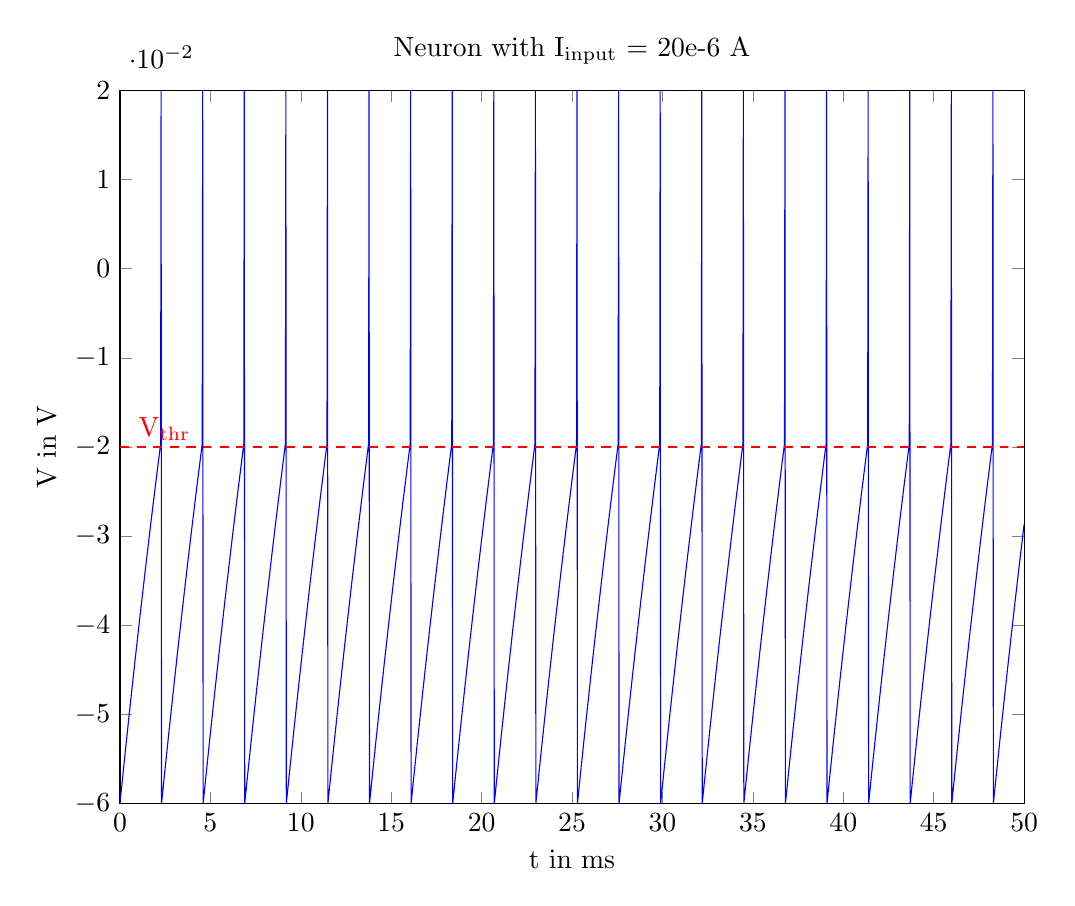
\begin{tikzpicture}

\begin{axis}[%
width=4.520833in,
height=3.565625in,
at={(0.758333in,0.48125in)},
scale only axis,
separate axis lines,
every outer x axis line/.append style={black},
every x tick label/.append style={font=\color{black}},
xmin=0,
xmax=50,
xlabel={t in ms},
every outer y axis line/.append style={black},
every y tick label/.append style={font=\color{black}},
ymin=-0.06,
ymax=0.02,
ylabel={V in V},
title={$\text{Neuron with I}_{\text{input}}\text{ = 20e-6 A}$}
]
\addplot [color=blue,solid,forget plot]
  table[row sep=crcr]{%
0	-0.06\\
0.025	-0.0595\\
0.05	-0.05900125\\
0.075	-0.058503746875\\
0.1	-0.0580074875078125\\
0.125	-0.057512468789043\\
0.15	-0.0570186876170704\\
0.175	-0.0565261408980277\\
0.2	-0.0560348255457826\\
0.225	-0.0555447384819182\\
0.25	-0.0550558766357134\\
0.275	-0.0545682369441241\\
0.3	-0.0540818163517638\\
0.325	-0.0535966118108844\\
0.35	-0.0531126202813572\\
0.375	-0.0526298387306538\\
0.4	-0.0521482641338271\\
0.425	-0.0516678934734926\\
0.45	-0.0511887237398088\\
0.475	-0.0507107519304593\\
0.5	-0.0502339750506332\\
0.525	-0.0497583901130066\\
0.55	-0.0492839941377241\\
0.575	-0.0488107841523797\\
0.6	-0.0483387571919988\\
0.625	-0.0478679102990188\\
0.65	-0.0473982405232712\\
0.675	-0.0469297449219631\\
0.7	-0.0464624205596582\\
0.725	-0.045996264508259\\
0.75	-0.0455312738469884\\
0.775	-0.0450674456623709\\
0.8	-0.044604777048215\\
0.825	-0.0441432651055944\\
0.85	-0.0436829069428305\\
0.875	-0.0432236996754734\\
0.9	-0.0427656404262847\\
0.925	-0.042308726325219\\
0.95	-0.0418529545094059\\
0.975	-0.0413983221231324\\
1	-0.0409448263178246\\
1.025	-0.04049246425203\\
1.05	-0.0400412330913999\\
1.075	-0.0395911300086714\\
1.1	-0.0391421521836498\\
1.125	-0.0386942968031906\\
1.15	-0.0382475610611827\\
1.175	-0.0378019421585297\\
1.2	-0.0373574373031334\\
1.225	-0.0369140437098756\\
1.25	-0.0364717586006009\\
1.275	-0.0360305792040994\\
1.3	-0.0355905027560891\\
1.325	-0.0351515264991989\\
1.35	-0.0347136476829509\\
1.375	-0.0342768635637435\\
1.4	-0.0338411714048342\\
1.425	-0.0334065684763221\\
1.45	-0.0329730520551313\\
1.475	-0.0325406194249934\\
1.5	-0.032109267876431\\
1.525	-0.0316789947067399\\
1.55	-0.031249797219973\\
1.575	-0.0308216727269231\\
1.6	-0.0303946185451058\\
1.625	-0.029968631998743\\
1.65	-0.0295437104187462\\
1.675	-0.0291198511426993\\
1.7	-0.0286970515148426\\
1.725	-0.0282753088860555\\
1.75	-0.0278546206138403\\
1.775	-0.0274349840623057\\
1.8	-0.0270163966021499\\
1.825	-0.0265988556106446\\
1.85	-0.026182358471618\\
1.875	-0.0257669025754389\\
1.9	-0.0253524853190003\\
1.925	-0.0249391041057028\\
1.95	-0.0245267563454386\\
1.975	-0.024115439454575\\
2	-0.0237051508559385\\
2.025	-0.0232958879787987\\
2.05	-0.0228876482588517\\
2.075	-0.0224804291382046\\
2.1	-0.022074228065359\\
2.125	-0.0216690424951956\\
2.15	-0.0212648698889577\\
2.175	-0.0208617077142353\\
2.2	-0.0204595534449497\\
2.225	-0.0200584045613373\\
2.25	-0.019658258549934\\
2.275	0.02\\
2.3	-0.06\\
2.325	-0.0595\\
2.35	-0.05900125\\
2.375	-0.058503746875\\
2.4	-0.0580074875078125\\
2.425	-0.057512468789043\\
2.45	-0.0570186876170704\\
2.475	-0.0565261408980277\\
2.5	-0.0560348255457826\\
2.525	-0.0555447384819182\\
2.55	-0.0550558766357134\\
2.575	-0.0545682369441241\\
2.6	-0.0540818163517638\\
2.625	-0.0535966118108844\\
2.65	-0.0531126202813572\\
2.675	-0.0526298387306538\\
2.7	-0.0521482641338271\\
2.725	-0.0516678934734926\\
2.75	-0.0511887237398088\\
2.775	-0.0507107519304593\\
2.8	-0.0502339750506332\\
2.825	-0.0497583901130066\\
2.85	-0.0492839941377241\\
2.875	-0.0488107841523797\\
2.9	-0.0483387571919988\\
2.925	-0.0478679102990188\\
2.95	-0.0473982405232712\\
2.975	-0.0469297449219631\\
3	-0.0464624205596582\\
3.025	-0.045996264508259\\
3.05	-0.0455312738469884\\
3.075	-0.0450674456623709\\
3.1	-0.044604777048215\\
3.125	-0.0441432651055944\\
3.15	-0.0436829069428305\\
3.175	-0.0432236996754734\\
3.2	-0.0427656404262847\\
3.225	-0.042308726325219\\
3.25	-0.0418529545094059\\
3.275	-0.0413983221231324\\
3.3	-0.0409448263178246\\
3.325	-0.04049246425203\\
3.35	-0.0400412330913999\\
3.375	-0.0395911300086714\\
3.4	-0.0391421521836498\\
3.425	-0.0386942968031906\\
3.45	-0.0382475610611827\\
3.475	-0.0378019421585297\\
3.5	-0.0373574373031334\\
3.525	-0.0369140437098756\\
3.55	-0.0364717586006009\\
3.575	-0.0360305792040994\\
3.6	-0.0355905027560891\\
3.625	-0.0351515264991989\\
3.65	-0.0347136476829509\\
3.675	-0.0342768635637435\\
3.7	-0.0338411714048342\\
3.725	-0.0334065684763221\\
3.75	-0.0329730520551313\\
3.775	-0.0325406194249934\\
3.8	-0.032109267876431\\
3.825	-0.0316789947067399\\
3.85	-0.031249797219973\\
3.875	-0.0308216727269231\\
3.9	-0.0303946185451058\\
3.925	-0.029968631998743\\
3.95	-0.0295437104187462\\
3.975	-0.0291198511426993\\
4	-0.0286970515148426\\
4.025	-0.0282753088860555\\
4.05	-0.0278546206138403\\
4.075	-0.0274349840623057\\
4.1	-0.0270163966021499\\
4.125	-0.0265988556106446\\
4.15	-0.026182358471618\\
4.175	-0.0257669025754389\\
4.2	-0.0253524853190003\\
4.225	-0.0249391041057028\\
4.25	-0.0245267563454386\\
4.275	-0.024115439454575\\
4.3	-0.0237051508559385\\
4.325	-0.0232958879787987\\
4.35	-0.0228876482588517\\
4.375	-0.0224804291382046\\
4.4	-0.022074228065359\\
4.425	-0.0216690424951956\\
4.45	-0.0212648698889577\\
4.475	-0.0208617077142353\\
4.5	-0.0204595534449497\\
4.525	-0.0200584045613373\\
4.55	-0.019658258549934\\
4.575	0.02\\
4.6	-0.06\\
4.625	-0.0595\\
4.65	-0.05900125\\
4.675	-0.058503746875\\
4.7	-0.0580074875078125\\
4.725	-0.057512468789043\\
4.75	-0.0570186876170704\\
4.775	-0.0565261408980277\\
4.8	-0.0560348255457826\\
4.825	-0.0555447384819182\\
4.85	-0.0550558766357134\\
4.875	-0.0545682369441241\\
4.9	-0.0540818163517638\\
4.925	-0.0535966118108844\\
4.95	-0.0531126202813572\\
4.975	-0.0526298387306538\\
5	-0.0521482641338271\\
5.025	-0.0516678934734926\\
5.05	-0.0511887237398088\\
5.075	-0.0507107519304593\\
5.1	-0.0502339750506332\\
5.125	-0.0497583901130066\\
5.15	-0.0492839941377241\\
5.175	-0.0488107841523797\\
5.2	-0.0483387571919988\\
5.225	-0.0478679102990188\\
5.25	-0.0473982405232712\\
5.275	-0.0469297449219631\\
5.3	-0.0464624205596582\\
5.325	-0.045996264508259\\
5.35	-0.0455312738469884\\
5.375	-0.0450674456623709\\
5.4	-0.044604777048215\\
5.425	-0.0441432651055944\\
5.45	-0.0436829069428305\\
5.475	-0.0432236996754734\\
5.5	-0.0427656404262847\\
5.525	-0.042308726325219\\
5.55	-0.0418529545094059\\
5.575	-0.0413983221231324\\
5.6	-0.0409448263178246\\
5.625	-0.04049246425203\\
5.65	-0.0400412330913999\\
5.675	-0.0395911300086714\\
5.7	-0.0391421521836498\\
5.725	-0.0386942968031906\\
5.75	-0.0382475610611827\\
5.775	-0.0378019421585297\\
5.8	-0.0373574373031334\\
5.825	-0.0369140437098756\\
5.85	-0.0364717586006009\\
5.875	-0.0360305792040994\\
5.9	-0.0355905027560891\\
5.925	-0.0351515264991989\\
5.95	-0.0347136476829509\\
5.975	-0.0342768635637435\\
6	-0.0338411714048342\\
6.025	-0.0334065684763221\\
6.05	-0.0329730520551313\\
6.075	-0.0325406194249934\\
6.1	-0.032109267876431\\
6.125	-0.0316789947067399\\
6.15	-0.031249797219973\\
6.175	-0.0308216727269231\\
6.2	-0.0303946185451058\\
6.225	-0.029968631998743\\
6.25	-0.0295437104187462\\
6.275	-0.0291198511426993\\
6.3	-0.0286970515148426\\
6.325	-0.0282753088860555\\
6.35	-0.0278546206138403\\
6.375	-0.0274349840623057\\
6.4	-0.0270163966021499\\
6.425	-0.0265988556106446\\
6.45	-0.026182358471618\\
6.475	-0.0257669025754389\\
6.5	-0.0253524853190003\\
6.525	-0.0249391041057028\\
6.55	-0.0245267563454386\\
6.575	-0.024115439454575\\
6.6	-0.0237051508559385\\
6.625	-0.0232958879787987\\
6.65	-0.0228876482588517\\
6.675	-0.0224804291382046\\
6.7	-0.022074228065359\\
6.725	-0.0216690424951956\\
6.75	-0.0212648698889577\\
6.775	-0.0208617077142353\\
6.8	-0.0204595534449497\\
6.825	-0.0200584045613373\\
6.85	-0.019658258549934\\
6.875	0.02\\
6.9	-0.06\\
6.925	-0.0595\\
6.95	-0.05900125\\
6.975	-0.058503746875\\
7	-0.0580074875078125\\
7.025	-0.057512468789043\\
7.05	-0.0570186876170704\\
7.075	-0.0565261408980277\\
7.1	-0.0560348255457826\\
7.125	-0.0555447384819182\\
7.15	-0.0550558766357134\\
7.175	-0.0545682369441241\\
7.2	-0.0540818163517638\\
7.225	-0.0535966118108844\\
7.25	-0.0531126202813572\\
7.275	-0.0526298387306538\\
7.3	-0.0521482641338271\\
7.325	-0.0516678934734926\\
7.35	-0.0511887237398088\\
7.375	-0.0507107519304593\\
7.4	-0.0502339750506332\\
7.425	-0.0497583901130066\\
7.45	-0.0492839941377241\\
7.475	-0.0488107841523797\\
7.5	-0.0483387571919988\\
7.525	-0.0478679102990188\\
7.55	-0.0473982405232712\\
7.575	-0.0469297449219631\\
7.6	-0.0464624205596582\\
7.625	-0.045996264508259\\
7.65	-0.0455312738469884\\
7.675	-0.0450674456623709\\
7.7	-0.044604777048215\\
7.725	-0.0441432651055944\\
7.75	-0.0436829069428305\\
7.775	-0.0432236996754734\\
7.8	-0.0427656404262847\\
7.825	-0.042308726325219\\
7.85	-0.0418529545094059\\
7.875	-0.0413983221231324\\
7.9	-0.0409448263178246\\
7.925	-0.04049246425203\\
7.95	-0.0400412330913999\\
7.975	-0.0395911300086714\\
8	-0.0391421521836498\\
8.025	-0.0386942968031906\\
8.05	-0.0382475610611827\\
8.075	-0.0378019421585297\\
8.1	-0.0373574373031334\\
8.125	-0.0369140437098756\\
8.15	-0.0364717586006009\\
8.175	-0.0360305792040994\\
8.2	-0.0355905027560891\\
8.225	-0.0351515264991989\\
8.25	-0.0347136476829509\\
8.275	-0.0342768635637435\\
8.3	-0.0338411714048342\\
8.325	-0.0334065684763221\\
8.35	-0.0329730520551313\\
8.375	-0.0325406194249934\\
8.4	-0.032109267876431\\
8.425	-0.0316789947067399\\
8.45	-0.031249797219973\\
8.475	-0.0308216727269231\\
8.5	-0.0303946185451058\\
8.525	-0.029968631998743\\
8.55	-0.0295437104187462\\
8.575	-0.0291198511426993\\
8.6	-0.0286970515148426\\
8.625	-0.0282753088860555\\
8.65	-0.0278546206138403\\
8.675	-0.0274349840623057\\
8.7	-0.0270163966021499\\
8.725	-0.0265988556106446\\
8.75	-0.026182358471618\\
8.775	-0.0257669025754389\\
8.8	-0.0253524853190003\\
8.825	-0.0249391041057028\\
8.85	-0.0245267563454386\\
8.875	-0.024115439454575\\
8.9	-0.0237051508559385\\
8.925	-0.0232958879787987\\
8.95	-0.0228876482588517\\
8.975	-0.0224804291382046\\
9	-0.022074228065359\\
9.025	-0.0216690424951956\\
9.05	-0.0212648698889577\\
9.075	-0.0208617077142353\\
9.1	-0.0204595534449497\\
9.125	-0.0200584045613373\\
9.15	-0.019658258549934\\
9.175	0.02\\
9.2	-0.06\\
9.225	-0.0595\\
9.25	-0.05900125\\
9.275	-0.058503746875\\
9.3	-0.0580074875078125\\
9.325	-0.057512468789043\\
9.35	-0.0570186876170704\\
9.375	-0.0565261408980277\\
9.4	-0.0560348255457826\\
9.425	-0.0555447384819182\\
9.45	-0.0550558766357134\\
9.475	-0.0545682369441241\\
9.5	-0.0540818163517638\\
9.525	-0.0535966118108844\\
9.55	-0.0531126202813572\\
9.575	-0.0526298387306538\\
9.6	-0.0521482641338271\\
9.625	-0.0516678934734926\\
9.65	-0.0511887237398088\\
9.675	-0.0507107519304593\\
9.7	-0.0502339750506332\\
9.725	-0.0497583901130066\\
9.75	-0.0492839941377241\\
9.775	-0.0488107841523797\\
9.8	-0.0483387571919988\\
9.825	-0.0478679102990188\\
9.85	-0.0473982405232712\\
9.875	-0.0469297449219631\\
9.9	-0.0464624205596582\\
9.925	-0.045996264508259\\
9.95	-0.0455312738469884\\
9.975	-0.0450674456623709\\
10	-0.044604777048215\\
10.025	-0.0441432651055944\\
10.05	-0.0436829069428305\\
10.075	-0.0432236996754734\\
10.1	-0.0427656404262847\\
10.125	-0.042308726325219\\
10.15	-0.0418529545094059\\
10.175	-0.0413983221231324\\
10.2	-0.0409448263178246\\
10.225	-0.04049246425203\\
10.25	-0.0400412330913999\\
10.275	-0.0395911300086714\\
10.3	-0.0391421521836498\\
10.325	-0.0386942968031906\\
10.35	-0.0382475610611827\\
10.375	-0.0378019421585297\\
10.4	-0.0373574373031334\\
10.425	-0.0369140437098756\\
10.45	-0.0364717586006009\\
10.475	-0.0360305792040994\\
10.5	-0.0355905027560891\\
10.525	-0.0351515264991989\\
10.55	-0.0347136476829509\\
10.575	-0.0342768635637435\\
10.6	-0.0338411714048342\\
10.625	-0.0334065684763221\\
10.65	-0.0329730520551313\\
10.675	-0.0325406194249934\\
10.7	-0.032109267876431\\
10.725	-0.0316789947067399\\
10.75	-0.031249797219973\\
10.775	-0.0308216727269231\\
10.8	-0.0303946185451058\\
10.825	-0.029968631998743\\
10.85	-0.0295437104187462\\
10.875	-0.0291198511426993\\
10.9	-0.0286970515148426\\
10.925	-0.0282753088860555\\
10.95	-0.0278546206138403\\
10.975	-0.0274349840623057\\
11	-0.0270163966021499\\
11.025	-0.0265988556106446\\
11.05	-0.026182358471618\\
11.075	-0.0257669025754389\\
11.1	-0.0253524853190003\\
11.125	-0.0249391041057028\\
11.15	-0.0245267563454386\\
11.175	-0.024115439454575\\
11.2	-0.0237051508559385\\
11.225	-0.0232958879787987\\
11.25	-0.0228876482588517\\
11.275	-0.0224804291382046\\
11.3	-0.022074228065359\\
11.325	-0.0216690424951956\\
11.35	-0.0212648698889577\\
11.375	-0.0208617077142353\\
11.4	-0.0204595534449497\\
11.425	-0.0200584045613373\\
11.45	-0.019658258549934\\
11.475	0.02\\
11.5	-0.06\\
11.525	-0.0595\\
11.55	-0.05900125\\
11.575	-0.058503746875\\
11.6	-0.0580074875078125\\
11.625	-0.057512468789043\\
11.65	-0.0570186876170704\\
11.675	-0.0565261408980277\\
11.7	-0.0560348255457826\\
11.725	-0.0555447384819182\\
11.75	-0.0550558766357134\\
11.775	-0.0545682369441241\\
11.8	-0.0540818163517638\\
11.825	-0.0535966118108844\\
11.85	-0.0531126202813572\\
11.875	-0.0526298387306538\\
11.9	-0.0521482641338271\\
11.925	-0.0516678934734926\\
11.95	-0.0511887237398088\\
11.975	-0.0507107519304593\\
12	-0.0502339750506332\\
12.025	-0.0497583901130066\\
12.05	-0.0492839941377241\\
12.075	-0.0488107841523797\\
12.1	-0.0483387571919988\\
12.125	-0.0478679102990188\\
12.15	-0.0473982405232712\\
12.175	-0.0469297449219631\\
12.2	-0.0464624205596582\\
12.225	-0.045996264508259\\
12.25	-0.0455312738469884\\
12.275	-0.0450674456623709\\
12.3	-0.044604777048215\\
12.325	-0.0441432651055944\\
12.35	-0.0436829069428305\\
12.375	-0.0432236996754734\\
12.4	-0.0427656404262847\\
12.425	-0.042308726325219\\
12.45	-0.0418529545094059\\
12.475	-0.0413983221231324\\
12.5	-0.0409448263178246\\
12.525	-0.04049246425203\\
12.55	-0.0400412330913999\\
12.575	-0.0395911300086714\\
12.6	-0.0391421521836498\\
12.625	-0.0386942968031906\\
12.65	-0.0382475610611827\\
12.675	-0.0378019421585297\\
12.7	-0.0373574373031334\\
12.725	-0.0369140437098756\\
12.75	-0.0364717586006009\\
12.775	-0.0360305792040994\\
12.8	-0.0355905027560891\\
12.825	-0.0351515264991989\\
12.85	-0.0347136476829509\\
12.875	-0.0342768635637435\\
12.9	-0.0338411714048342\\
12.925	-0.0334065684763221\\
12.95	-0.0329730520551313\\
12.975	-0.0325406194249934\\
13	-0.032109267876431\\
13.025	-0.0316789947067399\\
13.05	-0.031249797219973\\
13.075	-0.0308216727269231\\
13.1	-0.0303946185451058\\
13.125	-0.029968631998743\\
13.15	-0.0295437104187462\\
13.175	-0.0291198511426993\\
13.2	-0.0286970515148426\\
13.225	-0.0282753088860555\\
13.25	-0.0278546206138403\\
13.275	-0.0274349840623057\\
13.3	-0.0270163966021499\\
13.325	-0.0265988556106446\\
13.35	-0.026182358471618\\
13.375	-0.0257669025754389\\
13.4	-0.0253524853190003\\
13.425	-0.0249391041057028\\
13.45	-0.0245267563454386\\
13.475	-0.024115439454575\\
13.5	-0.0237051508559385\\
13.525	-0.0232958879787987\\
13.55	-0.0228876482588517\\
13.575	-0.0224804291382046\\
13.6	-0.022074228065359\\
13.625	-0.0216690424951956\\
13.65	-0.0212648698889577\\
13.675	-0.0208617077142353\\
13.7	-0.0204595534449497\\
13.725	-0.0200584045613373\\
13.75	-0.019658258549934\\
13.775	0.02\\
13.8	-0.06\\
13.825	-0.0595\\
13.85	-0.05900125\\
13.875	-0.058503746875\\
13.9	-0.0580074875078125\\
13.925	-0.057512468789043\\
13.95	-0.0570186876170704\\
13.975	-0.0565261408980277\\
14	-0.0560348255457826\\
14.025	-0.0555447384819182\\
14.05	-0.0550558766357134\\
14.075	-0.0545682369441241\\
14.1	-0.0540818163517638\\
14.125	-0.0535966118108844\\
14.15	-0.0531126202813572\\
14.175	-0.0526298387306538\\
14.2	-0.0521482641338271\\
14.225	-0.0516678934734926\\
14.25	-0.0511887237398088\\
14.275	-0.0507107519304593\\
14.3	-0.0502339750506332\\
14.325	-0.0497583901130066\\
14.35	-0.0492839941377241\\
14.375	-0.0488107841523797\\
14.4	-0.0483387571919988\\
14.425	-0.0478679102990188\\
14.45	-0.0473982405232712\\
14.475	-0.0469297449219631\\
14.5	-0.0464624205596582\\
14.525	-0.045996264508259\\
14.55	-0.0455312738469884\\
14.575	-0.0450674456623709\\
14.6	-0.044604777048215\\
14.625	-0.0441432651055944\\
14.65	-0.0436829069428305\\
14.675	-0.0432236996754734\\
14.7	-0.0427656404262847\\
14.725	-0.042308726325219\\
14.75	-0.0418529545094059\\
14.775	-0.0413983221231324\\
14.8	-0.0409448263178246\\
14.825	-0.04049246425203\\
14.85	-0.0400412330913999\\
14.875	-0.0395911300086714\\
14.9	-0.0391421521836498\\
14.925	-0.0386942968031906\\
14.95	-0.0382475610611827\\
14.975	-0.0378019421585297\\
15	-0.0373574373031334\\
15.025	-0.0369140437098756\\
15.05	-0.0364717586006009\\
15.075	-0.0360305792040994\\
15.1	-0.0355905027560891\\
15.125	-0.0351515264991989\\
15.15	-0.0347136476829509\\
15.175	-0.0342768635637435\\
15.2	-0.0338411714048342\\
15.225	-0.0334065684763221\\
15.25	-0.0329730520551313\\
15.275	-0.0325406194249934\\
15.3	-0.032109267876431\\
15.325	-0.0316789947067399\\
15.35	-0.031249797219973\\
15.375	-0.0308216727269231\\
15.4	-0.0303946185451058\\
15.425	-0.029968631998743\\
15.45	-0.0295437104187462\\
15.475	-0.0291198511426993\\
15.5	-0.0286970515148426\\
15.525	-0.0282753088860555\\
15.55	-0.0278546206138403\\
15.575	-0.0274349840623057\\
15.6	-0.0270163966021499\\
15.625	-0.0265988556106446\\
15.65	-0.026182358471618\\
15.675	-0.0257669025754389\\
15.7	-0.0253524853190003\\
15.725	-0.0249391041057028\\
15.75	-0.0245267563454386\\
15.775	-0.024115439454575\\
15.8	-0.0237051508559385\\
15.825	-0.0232958879787987\\
15.85	-0.0228876482588517\\
15.875	-0.0224804291382046\\
15.9	-0.022074228065359\\
15.925	-0.0216690424951956\\
15.95	-0.0212648698889577\\
15.975	-0.0208617077142353\\
16	-0.0204595534449497\\
16.025	-0.0200584045613373\\
16.05	-0.019658258549934\\
16.075	0.02\\
16.1	-0.06\\
16.125	-0.0595\\
16.15	-0.05900125\\
16.175	-0.058503746875\\
16.2	-0.0580074875078125\\
16.225	-0.057512468789043\\
16.25	-0.0570186876170704\\
16.275	-0.0565261408980277\\
16.3	-0.0560348255457826\\
16.325	-0.0555447384819182\\
16.35	-0.0550558766357134\\
16.375	-0.0545682369441241\\
16.4	-0.0540818163517638\\
16.425	-0.0535966118108844\\
16.45	-0.0531126202813572\\
16.475	-0.0526298387306538\\
16.5	-0.0521482641338271\\
16.525	-0.0516678934734926\\
16.55	-0.0511887237398088\\
16.575	-0.0507107519304593\\
16.6	-0.0502339750506332\\
16.625	-0.0497583901130066\\
16.65	-0.0492839941377241\\
16.675	-0.0488107841523797\\
16.7	-0.0483387571919988\\
16.725	-0.0478679102990188\\
16.75	-0.0473982405232712\\
16.775	-0.0469297449219631\\
16.8	-0.0464624205596582\\
16.825	-0.045996264508259\\
16.85	-0.0455312738469884\\
16.875	-0.0450674456623709\\
16.9	-0.044604777048215\\
16.925	-0.0441432651055944\\
16.95	-0.0436829069428305\\
16.975	-0.0432236996754734\\
17	-0.0427656404262847\\
17.025	-0.042308726325219\\
17.05	-0.0418529545094059\\
17.075	-0.0413983221231324\\
17.1	-0.0409448263178246\\
17.125	-0.04049246425203\\
17.15	-0.0400412330913999\\
17.175	-0.0395911300086714\\
17.2	-0.0391421521836498\\
17.225	-0.0386942968031906\\
17.25	-0.0382475610611827\\
17.275	-0.0378019421585297\\
17.3	-0.0373574373031334\\
17.325	-0.0369140437098756\\
17.35	-0.0364717586006009\\
17.375	-0.0360305792040994\\
17.4	-0.0355905027560891\\
17.425	-0.0351515264991989\\
17.45	-0.0347136476829509\\
17.475	-0.0342768635637435\\
17.5	-0.0338411714048342\\
17.525	-0.0334065684763221\\
17.55	-0.0329730520551313\\
17.575	-0.0325406194249934\\
17.6	-0.032109267876431\\
17.625	-0.0316789947067399\\
17.65	-0.031249797219973\\
17.675	-0.0308216727269231\\
17.7	-0.0303946185451058\\
17.725	-0.029968631998743\\
17.75	-0.0295437104187462\\
17.775	-0.0291198511426993\\
17.8	-0.0286970515148426\\
17.825	-0.0282753088860555\\
17.85	-0.0278546206138403\\
17.875	-0.0274349840623057\\
17.9	-0.0270163966021499\\
17.925	-0.0265988556106446\\
17.95	-0.026182358471618\\
17.975	-0.0257669025754389\\
18	-0.0253524853190003\\
18.025	-0.0249391041057028\\
18.05	-0.0245267563454386\\
18.075	-0.024115439454575\\
18.1	-0.0237051508559385\\
18.125	-0.0232958879787987\\
18.15	-0.0228876482588517\\
18.175	-0.0224804291382046\\
18.2	-0.022074228065359\\
18.225	-0.0216690424951956\\
18.25	-0.0212648698889577\\
18.275	-0.0208617077142353\\
18.3	-0.0204595534449497\\
18.325	-0.0200584045613373\\
18.35	-0.019658258549934\\
18.375	0.02\\
18.4	-0.06\\
18.425	-0.0595\\
18.45	-0.05900125\\
18.475	-0.058503746875\\
18.5	-0.0580074875078125\\
18.525	-0.057512468789043\\
18.55	-0.0570186876170704\\
18.575	-0.0565261408980277\\
18.6	-0.0560348255457826\\
18.625	-0.0555447384819182\\
18.65	-0.0550558766357134\\
18.675	-0.0545682369441241\\
18.7	-0.0540818163517638\\
18.725	-0.0535966118108844\\
18.75	-0.0531126202813572\\
18.775	-0.0526298387306538\\
18.8	-0.0521482641338271\\
18.825	-0.0516678934734926\\
18.85	-0.0511887237398088\\
18.875	-0.0507107519304593\\
18.9	-0.0502339750506332\\
18.925	-0.0497583901130066\\
18.95	-0.0492839941377241\\
18.975	-0.0488107841523797\\
19	-0.0483387571919988\\
19.025	-0.0478679102990188\\
19.05	-0.0473982405232712\\
19.075	-0.0469297449219631\\
19.1	-0.0464624205596582\\
19.125	-0.045996264508259\\
19.15	-0.0455312738469884\\
19.175	-0.0450674456623709\\
19.2	-0.044604777048215\\
19.225	-0.0441432651055944\\
19.25	-0.0436829069428305\\
19.275	-0.0432236996754734\\
19.3	-0.0427656404262847\\
19.325	-0.042308726325219\\
19.35	-0.0418529545094059\\
19.375	-0.0413983221231324\\
19.4	-0.0409448263178246\\
19.425	-0.04049246425203\\
19.45	-0.0400412330913999\\
19.475	-0.0395911300086714\\
19.5	-0.0391421521836498\\
19.525	-0.0386942968031906\\
19.55	-0.0382475610611827\\
19.575	-0.0378019421585297\\
19.6	-0.0373574373031334\\
19.625	-0.0369140437098756\\
19.65	-0.0364717586006009\\
19.675	-0.0360305792040994\\
19.7	-0.0355905027560891\\
19.725	-0.0351515264991989\\
19.75	-0.0347136476829509\\
19.775	-0.0342768635637435\\
19.8	-0.0338411714048342\\
19.825	-0.0334065684763221\\
19.85	-0.0329730520551313\\
19.875	-0.0325406194249934\\
19.9	-0.032109267876431\\
19.925	-0.0316789947067399\\
19.95	-0.031249797219973\\
19.975	-0.0308216727269231\\
20	-0.0303946185451058\\
20.025	-0.029968631998743\\
20.05	-0.0295437104187462\\
20.075	-0.0291198511426993\\
20.1	-0.0286970515148426\\
20.125	-0.0282753088860555\\
20.15	-0.0278546206138403\\
20.175	-0.0274349840623057\\
20.2	-0.0270163966021499\\
20.225	-0.0265988556106446\\
20.25	-0.026182358471618\\
20.275	-0.0257669025754389\\
20.3	-0.0253524853190003\\
20.325	-0.0249391041057028\\
20.35	-0.0245267563454386\\
20.375	-0.024115439454575\\
20.4	-0.0237051508559385\\
20.425	-0.0232958879787987\\
20.45	-0.0228876482588517\\
20.475	-0.0224804291382046\\
20.5	-0.022074228065359\\
20.525	-0.0216690424951956\\
20.55	-0.0212648698889577\\
20.575	-0.0208617077142353\\
20.6	-0.0204595534449497\\
20.625	-0.0200584045613373\\
20.65	-0.019658258549934\\
20.675	0.02\\
20.7	-0.06\\
20.725	-0.0595\\
20.75	-0.05900125\\
20.775	-0.058503746875\\
20.8	-0.0580074875078125\\
20.825	-0.057512468789043\\
20.85	-0.0570186876170704\\
20.875	-0.0565261408980277\\
20.9	-0.0560348255457826\\
20.925	-0.0555447384819182\\
20.95	-0.0550558766357134\\
20.975	-0.0545682369441241\\
21	-0.0540818163517638\\
21.025	-0.0535966118108844\\
21.05	-0.0531126202813572\\
21.075	-0.0526298387306538\\
21.1	-0.0521482641338271\\
21.125	-0.0516678934734926\\
21.15	-0.0511887237398088\\
21.175	-0.0507107519304593\\
21.2	-0.0502339750506332\\
21.225	-0.0497583901130066\\
21.25	-0.0492839941377241\\
21.275	-0.0488107841523797\\
21.3	-0.0483387571919988\\
21.325	-0.0478679102990188\\
21.35	-0.0473982405232712\\
21.375	-0.0469297449219631\\
21.4	-0.0464624205596582\\
21.425	-0.045996264508259\\
21.45	-0.0455312738469884\\
21.475	-0.0450674456623709\\
21.5	-0.044604777048215\\
21.525	-0.0441432651055944\\
21.55	-0.0436829069428305\\
21.575	-0.0432236996754734\\
21.6	-0.0427656404262847\\
21.625	-0.042308726325219\\
21.65	-0.0418529545094059\\
21.675	-0.0413983221231324\\
21.7	-0.0409448263178246\\
21.725	-0.04049246425203\\
21.75	-0.0400412330913999\\
21.775	-0.0395911300086714\\
21.8	-0.0391421521836498\\
21.825	-0.0386942968031906\\
21.85	-0.0382475610611827\\
21.875	-0.0378019421585297\\
21.9	-0.0373574373031334\\
21.925	-0.0369140437098756\\
21.95	-0.0364717586006009\\
21.975	-0.0360305792040994\\
22	-0.0355905027560891\\
22.025	-0.0351515264991989\\
22.05	-0.0347136476829509\\
22.075	-0.0342768635637435\\
22.1	-0.0338411714048342\\
22.125	-0.0334065684763221\\
22.15	-0.0329730520551313\\
22.175	-0.0325406194249934\\
22.2	-0.032109267876431\\
22.225	-0.0316789947067399\\
22.25	-0.031249797219973\\
22.275	-0.0308216727269231\\
22.3	-0.0303946185451058\\
22.325	-0.029968631998743\\
22.35	-0.0295437104187462\\
22.375	-0.0291198511426993\\
22.4	-0.0286970515148426\\
22.425	-0.0282753088860555\\
22.45	-0.0278546206138403\\
22.475	-0.0274349840623057\\
22.5	-0.0270163966021499\\
22.525	-0.0265988556106446\\
22.55	-0.026182358471618\\
22.575	-0.0257669025754389\\
22.6	-0.0253524853190003\\
22.625	-0.0249391041057028\\
22.65	-0.0245267563454386\\
22.675	-0.024115439454575\\
22.7	-0.0237051508559385\\
22.725	-0.0232958879787987\\
22.75	-0.0228876482588517\\
22.775	-0.0224804291382046\\
22.8	-0.022074228065359\\
22.825	-0.0216690424951956\\
22.85	-0.0212648698889577\\
22.875	-0.0208617077142353\\
22.9	-0.0204595534449497\\
22.925	-0.0200584045613373\\
22.95	-0.019658258549934\\
22.975	0.02\\
23	-0.06\\
23.025	-0.0595\\
23.05	-0.05900125\\
23.075	-0.058503746875\\
23.1	-0.0580074875078125\\
23.125	-0.057512468789043\\
23.15	-0.0570186876170704\\
23.175	-0.0565261408980277\\
23.2	-0.0560348255457826\\
23.225	-0.0555447384819182\\
23.25	-0.0550558766357134\\
23.275	-0.0545682369441241\\
23.3	-0.0540818163517638\\
23.325	-0.0535966118108844\\
23.35	-0.0531126202813572\\
23.375	-0.0526298387306538\\
23.4	-0.0521482641338271\\
23.425	-0.0516678934734926\\
23.45	-0.0511887237398088\\
23.475	-0.0507107519304593\\
23.5	-0.0502339750506332\\
23.525	-0.0497583901130066\\
23.55	-0.0492839941377241\\
23.575	-0.0488107841523797\\
23.6	-0.0483387571919988\\
23.625	-0.0478679102990188\\
23.65	-0.0473982405232712\\
23.675	-0.0469297449219631\\
23.7	-0.0464624205596582\\
23.725	-0.045996264508259\\
23.75	-0.0455312738469884\\
23.775	-0.0450674456623709\\
23.8	-0.044604777048215\\
23.825	-0.0441432651055944\\
23.85	-0.0436829069428305\\
23.875	-0.0432236996754734\\
23.9	-0.0427656404262847\\
23.925	-0.042308726325219\\
23.95	-0.0418529545094059\\
23.975	-0.0413983221231324\\
24	-0.0409448263178246\\
24.025	-0.04049246425203\\
24.05	-0.0400412330913999\\
24.075	-0.0395911300086714\\
24.1	-0.0391421521836498\\
24.125	-0.0386942968031906\\
24.15	-0.0382475610611827\\
24.175	-0.0378019421585297\\
24.2	-0.0373574373031334\\
24.225	-0.0369140437098756\\
24.25	-0.0364717586006009\\
24.275	-0.0360305792040994\\
24.3	-0.0355905027560891\\
24.325	-0.0351515264991989\\
24.35	-0.0347136476829509\\
24.375	-0.0342768635637435\\
24.4	-0.0338411714048342\\
24.425	-0.0334065684763221\\
24.45	-0.0329730520551313\\
24.475	-0.0325406194249934\\
24.5	-0.032109267876431\\
24.525	-0.0316789947067399\\
24.55	-0.031249797219973\\
24.575	-0.0308216727269231\\
24.6	-0.0303946185451058\\
24.625	-0.029968631998743\\
24.65	-0.0295437104187462\\
24.675	-0.0291198511426993\\
24.7	-0.0286970515148426\\
24.725	-0.0282753088860555\\
24.75	-0.0278546206138403\\
24.775	-0.0274349840623057\\
24.8	-0.0270163966021499\\
24.825	-0.0265988556106446\\
24.85	-0.026182358471618\\
24.875	-0.0257669025754389\\
24.9	-0.0253524853190003\\
24.925	-0.0249391041057028\\
24.95	-0.0245267563454386\\
24.975	-0.024115439454575\\
25	-0.0237051508559385\\
25.025	-0.0232958879787987\\
25.05	-0.0228876482588517\\
25.075	-0.0224804291382046\\
25.1	-0.022074228065359\\
25.125	-0.0216690424951956\\
25.15	-0.0212648698889577\\
25.175	-0.0208617077142353\\
25.2	-0.0204595534449497\\
25.225	-0.0200584045613373\\
25.25	-0.019658258549934\\
25.275	0.02\\
25.3	-0.06\\
25.325	-0.0595\\
25.35	-0.05900125\\
25.375	-0.058503746875\\
25.4	-0.0580074875078125\\
25.425	-0.057512468789043\\
25.45	-0.0570186876170704\\
25.475	-0.0565261408980277\\
25.5	-0.0560348255457826\\
25.525	-0.0555447384819182\\
25.55	-0.0550558766357134\\
25.575	-0.0545682369441241\\
25.6	-0.0540818163517638\\
25.625	-0.0535966118108844\\
25.65	-0.0531126202813572\\
25.675	-0.0526298387306538\\
25.7	-0.0521482641338271\\
25.725	-0.0516678934734926\\
25.75	-0.0511887237398088\\
25.775	-0.0507107519304593\\
25.8	-0.0502339750506332\\
25.825	-0.0497583901130066\\
25.85	-0.0492839941377241\\
25.875	-0.0488107841523797\\
25.9	-0.0483387571919988\\
25.925	-0.0478679102990188\\
25.95	-0.0473982405232712\\
25.975	-0.0469297449219631\\
26	-0.0464624205596582\\
26.025	-0.045996264508259\\
26.05	-0.0455312738469884\\
26.075	-0.0450674456623709\\
26.1	-0.044604777048215\\
26.125	-0.0441432651055944\\
26.15	-0.0436829069428305\\
26.175	-0.0432236996754734\\
26.2	-0.0427656404262847\\
26.225	-0.042308726325219\\
26.25	-0.0418529545094059\\
26.275	-0.0413983221231324\\
26.3	-0.0409448263178246\\
26.325	-0.04049246425203\\
26.35	-0.0400412330913999\\
26.375	-0.0395911300086714\\
26.4	-0.0391421521836498\\
26.425	-0.0386942968031906\\
26.45	-0.0382475610611827\\
26.475	-0.0378019421585297\\
26.5	-0.0373574373031334\\
26.525	-0.0369140437098756\\
26.55	-0.0364717586006009\\
26.575	-0.0360305792040994\\
26.6	-0.0355905027560891\\
26.625	-0.0351515264991989\\
26.65	-0.0347136476829509\\
26.675	-0.0342768635637435\\
26.7	-0.0338411714048342\\
26.725	-0.0334065684763221\\
26.75	-0.0329730520551313\\
26.775	-0.0325406194249934\\
26.8	-0.032109267876431\\
26.825	-0.0316789947067399\\
26.85	-0.031249797219973\\
26.875	-0.0308216727269231\\
26.9	-0.0303946185451058\\
26.925	-0.029968631998743\\
26.95	-0.0295437104187462\\
26.975	-0.0291198511426993\\
27	-0.0286970515148426\\
27.025	-0.0282753088860555\\
27.05	-0.0278546206138403\\
27.075	-0.0274349840623057\\
27.1	-0.0270163966021499\\
27.125	-0.0265988556106446\\
27.15	-0.026182358471618\\
27.175	-0.0257669025754389\\
27.2	-0.0253524853190003\\
27.225	-0.0249391041057028\\
27.25	-0.0245267563454386\\
27.275	-0.024115439454575\\
27.3	-0.0237051508559385\\
27.325	-0.0232958879787987\\
27.35	-0.0228876482588517\\
27.375	-0.0224804291382046\\
27.4	-0.022074228065359\\
27.425	-0.0216690424951956\\
27.45	-0.0212648698889577\\
27.475	-0.0208617077142353\\
27.5	-0.0204595534449497\\
27.525	-0.0200584045613373\\
27.55	-0.019658258549934\\
27.575	0.02\\
27.6	-0.06\\
27.625	-0.0595\\
27.65	-0.05900125\\
27.675	-0.058503746875\\
27.7	-0.0580074875078125\\
27.725	-0.057512468789043\\
27.75	-0.0570186876170704\\
27.775	-0.0565261408980277\\
27.8	-0.0560348255457826\\
27.825	-0.0555447384819182\\
27.85	-0.0550558766357134\\
27.875	-0.0545682369441241\\
27.9	-0.0540818163517638\\
27.925	-0.0535966118108844\\
27.95	-0.0531126202813572\\
27.975	-0.0526298387306538\\
28	-0.0521482641338271\\
28.025	-0.0516678934734926\\
28.05	-0.0511887237398088\\
28.075	-0.0507107519304593\\
28.1	-0.0502339750506332\\
28.125	-0.0497583901130066\\
28.15	-0.0492839941377241\\
28.175	-0.0488107841523797\\
28.2	-0.0483387571919988\\
28.225	-0.0478679102990188\\
28.25	-0.0473982405232712\\
28.275	-0.0469297449219631\\
28.3	-0.0464624205596582\\
28.325	-0.045996264508259\\
28.35	-0.0455312738469884\\
28.375	-0.0450674456623709\\
28.4	-0.044604777048215\\
28.425	-0.0441432651055944\\
28.45	-0.0436829069428305\\
28.475	-0.0432236996754734\\
28.5	-0.0427656404262847\\
28.525	-0.042308726325219\\
28.55	-0.0418529545094059\\
28.575	-0.0413983221231324\\
28.6	-0.0409448263178246\\
28.625	-0.04049246425203\\
28.65	-0.0400412330913999\\
28.675	-0.0395911300086714\\
28.7	-0.0391421521836498\\
28.725	-0.0386942968031906\\
28.75	-0.0382475610611827\\
28.775	-0.0378019421585297\\
28.8	-0.0373574373031334\\
28.825	-0.0369140437098756\\
28.85	-0.0364717586006009\\
28.875	-0.0360305792040994\\
28.9	-0.0355905027560891\\
28.925	-0.0351515264991989\\
28.95	-0.0347136476829509\\
28.975	-0.0342768635637435\\
29	-0.0338411714048342\\
29.025	-0.0334065684763221\\
29.05	-0.0329730520551313\\
29.075	-0.0325406194249934\\
29.1	-0.032109267876431\\
29.125	-0.0316789947067399\\
29.15	-0.031249797219973\\
29.175	-0.0308216727269231\\
29.2	-0.0303946185451058\\
29.225	-0.029968631998743\\
29.25	-0.0295437104187462\\
29.275	-0.0291198511426993\\
29.3	-0.0286970515148426\\
29.325	-0.0282753088860555\\
29.35	-0.0278546206138403\\
29.375	-0.0274349840623057\\
29.4	-0.0270163966021499\\
29.425	-0.0265988556106446\\
29.45	-0.026182358471618\\
29.475	-0.0257669025754389\\
29.5	-0.0253524853190003\\
29.525	-0.0249391041057028\\
29.55	-0.0245267563454386\\
29.575	-0.024115439454575\\
29.6	-0.0237051508559385\\
29.625	-0.0232958879787987\\
29.65	-0.0228876482588517\\
29.675	-0.0224804291382046\\
29.7	-0.022074228065359\\
29.725	-0.0216690424951956\\
29.75	-0.0212648698889577\\
29.775	-0.0208617077142353\\
29.8	-0.0204595534449497\\
29.825	-0.0200584045613373\\
29.85	-0.019658258549934\\
29.875	0.02\\
29.9	-0.06\\
29.925	-0.0595\\
29.95	-0.05900125\\
29.975	-0.058503746875\\
30	-0.0580074875078125\\
30.025	-0.057512468789043\\
30.05	-0.0570186876170704\\
30.075	-0.0565261408980277\\
30.1	-0.0560348255457826\\
30.125	-0.0555447384819182\\
30.15	-0.0550558766357134\\
30.175	-0.0545682369441241\\
30.2	-0.0540818163517638\\
30.225	-0.0535966118108844\\
30.25	-0.0531126202813572\\
30.275	-0.0526298387306538\\
30.3	-0.0521482641338271\\
30.325	-0.0516678934734926\\
30.35	-0.0511887237398088\\
30.375	-0.0507107519304593\\
30.4	-0.0502339750506332\\
30.425	-0.0497583901130066\\
30.45	-0.0492839941377241\\
30.475	-0.0488107841523797\\
30.5	-0.0483387571919988\\
30.525	-0.0478679102990188\\
30.55	-0.0473982405232712\\
30.575	-0.0469297449219631\\
30.6	-0.0464624205596582\\
30.625	-0.045996264508259\\
30.65	-0.0455312738469884\\
30.675	-0.0450674456623709\\
30.7	-0.044604777048215\\
30.725	-0.0441432651055944\\
30.75	-0.0436829069428305\\
30.775	-0.0432236996754734\\
30.8	-0.0427656404262847\\
30.825	-0.042308726325219\\
30.85	-0.0418529545094059\\
30.875	-0.0413983221231324\\
30.9	-0.0409448263178246\\
30.925	-0.04049246425203\\
30.95	-0.0400412330913999\\
30.975	-0.0395911300086714\\
31	-0.0391421521836498\\
31.025	-0.0386942968031906\\
31.05	-0.0382475610611827\\
31.075	-0.0378019421585297\\
31.1	-0.0373574373031334\\
31.125	-0.0369140437098756\\
31.15	-0.0364717586006009\\
31.175	-0.0360305792040994\\
31.2	-0.0355905027560891\\
31.225	-0.0351515264991989\\
31.25	-0.0347136476829509\\
31.275	-0.0342768635637435\\
31.3	-0.0338411714048342\\
31.325	-0.0334065684763221\\
31.35	-0.0329730520551313\\
31.375	-0.0325406194249934\\
31.4	-0.032109267876431\\
31.425	-0.0316789947067399\\
31.45	-0.031249797219973\\
31.475	-0.0308216727269231\\
31.5	-0.0303946185451058\\
31.525	-0.029968631998743\\
31.55	-0.0295437104187462\\
31.575	-0.0291198511426993\\
31.6	-0.0286970515148426\\
31.625	-0.0282753088860555\\
31.65	-0.0278546206138403\\
31.675	-0.0274349840623057\\
31.7	-0.0270163966021499\\
31.725	-0.0265988556106446\\
31.75	-0.026182358471618\\
31.775	-0.0257669025754389\\
31.8	-0.0253524853190003\\
31.825	-0.0249391041057028\\
31.85	-0.0245267563454386\\
31.875	-0.024115439454575\\
31.9	-0.0237051508559385\\
31.925	-0.0232958879787987\\
31.95	-0.0228876482588517\\
31.975	-0.0224804291382046\\
32	-0.022074228065359\\
32.025	-0.0216690424951956\\
32.05	-0.0212648698889577\\
32.075	-0.0208617077142353\\
32.1	-0.0204595534449497\\
32.125	-0.0200584045613373\\
32.15	-0.019658258549934\\
32.175	0.02\\
32.2	-0.06\\
32.225	-0.0595\\
32.25	-0.05900125\\
32.275	-0.058503746875\\
32.3	-0.0580074875078125\\
32.325	-0.057512468789043\\
32.35	-0.0570186876170704\\
32.375	-0.0565261408980277\\
32.4	-0.0560348255457826\\
32.425	-0.0555447384819182\\
32.45	-0.0550558766357134\\
32.475	-0.0545682369441241\\
32.5	-0.0540818163517638\\
32.525	-0.0535966118108844\\
32.55	-0.0531126202813572\\
32.575	-0.0526298387306538\\
32.6	-0.0521482641338271\\
32.625	-0.0516678934734926\\
32.65	-0.0511887237398088\\
32.675	-0.0507107519304593\\
32.7	-0.0502339750506332\\
32.725	-0.0497583901130066\\
32.75	-0.0492839941377241\\
32.775	-0.0488107841523797\\
32.8	-0.0483387571919988\\
32.825	-0.0478679102990188\\
32.85	-0.0473982405232712\\
32.875	-0.0469297449219631\\
32.9	-0.0464624205596582\\
32.925	-0.045996264508259\\
32.95	-0.0455312738469884\\
32.975	-0.0450674456623709\\
33	-0.044604777048215\\
33.025	-0.0441432651055944\\
33.05	-0.0436829069428305\\
33.075	-0.0432236996754734\\
33.1	-0.0427656404262847\\
33.125	-0.042308726325219\\
33.15	-0.0418529545094059\\
33.175	-0.0413983221231324\\
33.2	-0.0409448263178246\\
33.225	-0.04049246425203\\
33.25	-0.0400412330913999\\
33.275	-0.0395911300086714\\
33.3	-0.0391421521836498\\
33.325	-0.0386942968031906\\
33.35	-0.0382475610611827\\
33.375	-0.0378019421585297\\
33.4	-0.0373574373031334\\
33.425	-0.0369140437098756\\
33.45	-0.0364717586006009\\
33.475	-0.0360305792040994\\
33.5	-0.0355905027560891\\
33.525	-0.0351515264991989\\
33.55	-0.0347136476829509\\
33.575	-0.0342768635637435\\
33.6	-0.0338411714048342\\
33.625	-0.0334065684763221\\
33.65	-0.0329730520551313\\
33.675	-0.0325406194249934\\
33.7	-0.032109267876431\\
33.725	-0.0316789947067399\\
33.75	-0.031249797219973\\
33.775	-0.0308216727269231\\
33.8	-0.0303946185451058\\
33.825	-0.029968631998743\\
33.85	-0.0295437104187462\\
33.875	-0.0291198511426993\\
33.9	-0.0286970515148426\\
33.925	-0.0282753088860555\\
33.95	-0.0278546206138403\\
33.975	-0.0274349840623057\\
34	-0.0270163966021499\\
34.025	-0.0265988556106446\\
34.05	-0.026182358471618\\
34.075	-0.0257669025754389\\
34.1	-0.0253524853190003\\
34.125	-0.0249391041057028\\
34.15	-0.0245267563454386\\
34.175	-0.024115439454575\\
34.2	-0.0237051508559385\\
34.225	-0.0232958879787987\\
34.25	-0.0228876482588517\\
34.275	-0.0224804291382046\\
34.3	-0.022074228065359\\
34.325	-0.0216690424951956\\
34.35	-0.0212648698889577\\
34.375	-0.0208617077142353\\
34.4	-0.0204595534449497\\
34.425	-0.0200584045613373\\
34.45	-0.019658258549934\\
34.475	0.02\\
34.5	-0.06\\
34.525	-0.0595\\
34.55	-0.05900125\\
34.575	-0.058503746875\\
34.6	-0.0580074875078125\\
34.625	-0.057512468789043\\
34.65	-0.0570186876170704\\
34.675	-0.0565261408980277\\
34.7	-0.0560348255457826\\
34.725	-0.0555447384819182\\
34.75	-0.0550558766357134\\
34.775	-0.0545682369441241\\
34.8	-0.0540818163517638\\
34.825	-0.0535966118108844\\
34.85	-0.0531126202813572\\
34.875	-0.0526298387306538\\
34.9	-0.0521482641338271\\
34.925	-0.0516678934734926\\
34.95	-0.0511887237398088\\
34.975	-0.0507107519304593\\
35	-0.0502339750506332\\
35.025	-0.0497583901130066\\
35.05	-0.0492839941377241\\
35.075	-0.0488107841523797\\
35.1	-0.0483387571919988\\
35.125	-0.0478679102990188\\
35.15	-0.0473982405232712\\
35.175	-0.0469297449219631\\
35.2	-0.0464624205596582\\
35.225	-0.045996264508259\\
35.25	-0.0455312738469884\\
35.275	-0.0450674456623709\\
35.3	-0.044604777048215\\
35.325	-0.0441432651055944\\
35.35	-0.0436829069428305\\
35.375	-0.0432236996754734\\
35.4	-0.0427656404262847\\
35.425	-0.042308726325219\\
35.45	-0.0418529545094059\\
35.475	-0.0413983221231324\\
35.5	-0.0409448263178246\\
35.525	-0.04049246425203\\
35.55	-0.0400412330913999\\
35.575	-0.0395911300086714\\
35.6	-0.0391421521836498\\
35.625	-0.0386942968031906\\
35.65	-0.0382475610611827\\
35.675	-0.0378019421585297\\
35.7	-0.0373574373031334\\
35.725	-0.0369140437098756\\
35.75	-0.0364717586006009\\
35.775	-0.0360305792040994\\
35.8	-0.0355905027560891\\
35.825	-0.0351515264991989\\
35.85	-0.0347136476829509\\
35.875	-0.0342768635637435\\
35.9	-0.0338411714048342\\
35.925	-0.0334065684763221\\
35.95	-0.0329730520551313\\
35.975	-0.0325406194249934\\
36	-0.032109267876431\\
36.025	-0.0316789947067399\\
36.05	-0.031249797219973\\
36.075	-0.0308216727269231\\
36.1	-0.0303946185451058\\
36.125	-0.029968631998743\\
36.15	-0.0295437104187462\\
36.175	-0.0291198511426993\\
36.2	-0.0286970515148426\\
36.225	-0.0282753088860555\\
36.25	-0.0278546206138403\\
36.275	-0.0274349840623057\\
36.3	-0.0270163966021499\\
36.325	-0.0265988556106446\\
36.35	-0.026182358471618\\
36.375	-0.0257669025754389\\
36.4	-0.0253524853190003\\
36.425	-0.0249391041057028\\
36.45	-0.0245267563454386\\
36.475	-0.024115439454575\\
36.5	-0.0237051508559385\\
36.525	-0.0232958879787987\\
36.55	-0.0228876482588517\\
36.575	-0.0224804291382046\\
36.6	-0.022074228065359\\
36.625	-0.0216690424951956\\
36.65	-0.0212648698889577\\
36.675	-0.0208617077142353\\
36.7	-0.0204595534449497\\
36.725	-0.0200584045613373\\
36.75	-0.019658258549934\\
36.775	0.02\\
36.8	-0.06\\
36.825	-0.0595\\
36.85	-0.05900125\\
36.875	-0.058503746875\\
36.9	-0.0580074875078125\\
36.925	-0.057512468789043\\
36.95	-0.0570186876170704\\
36.975	-0.0565261408980277\\
37	-0.0560348255457826\\
37.025	-0.0555447384819182\\
37.05	-0.0550558766357134\\
37.075	-0.0545682369441241\\
37.1	-0.0540818163517638\\
37.125	-0.0535966118108844\\
37.15	-0.0531126202813572\\
37.175	-0.0526298387306538\\
37.2	-0.0521482641338271\\
37.225	-0.0516678934734926\\
37.25	-0.0511887237398088\\
37.275	-0.0507107519304593\\
37.3	-0.0502339750506332\\
37.325	-0.0497583901130066\\
37.35	-0.0492839941377241\\
37.375	-0.0488107841523797\\
37.4	-0.0483387571919988\\
37.425	-0.0478679102990188\\
37.45	-0.0473982405232712\\
37.475	-0.0469297449219631\\
37.5	-0.0464624205596582\\
37.525	-0.045996264508259\\
37.55	-0.0455312738469884\\
37.575	-0.0450674456623709\\
37.6	-0.044604777048215\\
37.625	-0.0441432651055944\\
37.65	-0.0436829069428305\\
37.675	-0.0432236996754734\\
37.7	-0.0427656404262847\\
37.725	-0.042308726325219\\
37.75	-0.0418529545094059\\
37.775	-0.0413983221231324\\
37.8	-0.0409448263178246\\
37.825	-0.04049246425203\\
37.85	-0.0400412330913999\\
37.875	-0.0395911300086714\\
37.9	-0.0391421521836498\\
37.925	-0.0386942968031906\\
37.95	-0.0382475610611827\\
37.975	-0.0378019421585297\\
38	-0.0373574373031334\\
38.025	-0.0369140437098756\\
38.05	-0.0364717586006009\\
38.075	-0.0360305792040994\\
38.1	-0.0355905027560891\\
38.125	-0.0351515264991989\\
38.15	-0.0347136476829509\\
38.175	-0.0342768635637435\\
38.2	-0.0338411714048342\\
38.225	-0.0334065684763221\\
38.25	-0.0329730520551313\\
38.275	-0.0325406194249934\\
38.3	-0.032109267876431\\
38.325	-0.0316789947067399\\
38.35	-0.031249797219973\\
38.375	-0.0308216727269231\\
38.4	-0.0303946185451058\\
38.425	-0.029968631998743\\
38.45	-0.0295437104187462\\
38.475	-0.0291198511426993\\
38.5	-0.0286970515148426\\
38.525	-0.0282753088860555\\
38.55	-0.0278546206138403\\
38.575	-0.0274349840623057\\
38.6	-0.0270163966021499\\
38.625	-0.0265988556106446\\
38.65	-0.026182358471618\\
38.675	-0.0257669025754389\\
38.7	-0.0253524853190003\\
38.725	-0.0249391041057028\\
38.75	-0.0245267563454386\\
38.775	-0.024115439454575\\
38.8	-0.0237051508559385\\
38.825	-0.0232958879787987\\
38.85	-0.0228876482588517\\
38.875	-0.0224804291382046\\
38.9	-0.022074228065359\\
38.925	-0.0216690424951956\\
38.95	-0.0212648698889577\\
38.975	-0.0208617077142353\\
39	-0.0204595534449497\\
39.025	-0.0200584045613373\\
39.05	-0.019658258549934\\
39.075	0.02\\
39.1	-0.06\\
39.125	-0.0595\\
39.15	-0.05900125\\
39.175	-0.058503746875\\
39.2	-0.0580074875078125\\
39.225	-0.057512468789043\\
39.25	-0.0570186876170704\\
39.275	-0.0565261408980277\\
39.3	-0.0560348255457826\\
39.325	-0.0555447384819182\\
39.35	-0.0550558766357134\\
39.375	-0.0545682369441241\\
39.4	-0.0540818163517638\\
39.425	-0.0535966118108844\\
39.45	-0.0531126202813572\\
39.475	-0.0526298387306538\\
39.5	-0.0521482641338271\\
39.525	-0.0516678934734926\\
39.55	-0.0511887237398088\\
39.575	-0.0507107519304593\\
39.6	-0.0502339750506332\\
39.625	-0.0497583901130066\\
39.65	-0.0492839941377241\\
39.675	-0.0488107841523797\\
39.7	-0.0483387571919988\\
39.725	-0.0478679102990188\\
39.75	-0.0473982405232712\\
39.775	-0.0469297449219631\\
39.8	-0.0464624205596582\\
39.825	-0.045996264508259\\
39.85	-0.0455312738469884\\
39.875	-0.0450674456623709\\
39.9	-0.044604777048215\\
39.925	-0.0441432651055944\\
39.95	-0.0436829069428305\\
39.975	-0.0432236996754734\\
40	-0.0427656404262847\\
40.025	-0.042308726325219\\
40.05	-0.0418529545094059\\
40.075	-0.0413983221231324\\
40.1	-0.0409448263178246\\
40.125	-0.04049246425203\\
40.15	-0.0400412330913999\\
40.175	-0.0395911300086714\\
40.2	-0.0391421521836498\\
40.225	-0.0386942968031906\\
40.25	-0.0382475610611827\\
40.275	-0.0378019421585297\\
40.3	-0.0373574373031334\\
40.325	-0.0369140437098756\\
40.35	-0.0364717586006009\\
40.375	-0.0360305792040994\\
40.4	-0.0355905027560891\\
40.425	-0.0351515264991989\\
40.45	-0.0347136476829509\\
40.475	-0.0342768635637435\\
40.5	-0.0338411714048342\\
40.525	-0.0334065684763221\\
40.55	-0.0329730520551313\\
40.575	-0.0325406194249934\\
40.6	-0.032109267876431\\
40.625	-0.0316789947067399\\
40.65	-0.031249797219973\\
40.675	-0.0308216727269231\\
40.7	-0.0303946185451058\\
40.725	-0.029968631998743\\
40.75	-0.0295437104187462\\
40.775	-0.0291198511426993\\
40.8	-0.0286970515148426\\
40.825	-0.0282753088860555\\
40.85	-0.0278546206138403\\
40.875	-0.0274349840623057\\
40.9	-0.0270163966021499\\
40.925	-0.0265988556106446\\
40.95	-0.026182358471618\\
40.975	-0.0257669025754389\\
41	-0.0253524853190003\\
41.025	-0.0249391041057028\\
41.05	-0.0245267563454386\\
41.075	-0.024115439454575\\
41.1	-0.0237051508559385\\
41.125	-0.0232958879787987\\
41.15	-0.0228876482588517\\
41.175	-0.0224804291382046\\
41.2	-0.022074228065359\\
41.225	-0.0216690424951956\\
41.25	-0.0212648698889577\\
41.275	-0.0208617077142353\\
41.3	-0.0204595534449497\\
41.325	-0.0200584045613373\\
41.35	-0.019658258549934\\
41.375	0.02\\
41.4	-0.06\\
41.425	-0.0595\\
41.45	-0.05900125\\
41.475	-0.058503746875\\
41.5	-0.0580074875078125\\
41.525	-0.057512468789043\\
41.55	-0.0570186876170704\\
41.575	-0.0565261408980277\\
41.6	-0.0560348255457826\\
41.625	-0.0555447384819182\\
41.65	-0.0550558766357134\\
41.675	-0.0545682369441241\\
41.7	-0.0540818163517638\\
41.725	-0.0535966118108844\\
41.75	-0.0531126202813572\\
41.775	-0.0526298387306538\\
41.8	-0.0521482641338271\\
41.825	-0.0516678934734926\\
41.85	-0.0511887237398088\\
41.875	-0.0507107519304593\\
41.9	-0.0502339750506332\\
41.925	-0.0497583901130066\\
41.95	-0.0492839941377241\\
41.975	-0.0488107841523797\\
42	-0.0483387571919988\\
42.025	-0.0478679102990188\\
42.05	-0.0473982405232712\\
42.075	-0.0469297449219631\\
42.1	-0.0464624205596582\\
42.125	-0.045996264508259\\
42.15	-0.0455312738469884\\
42.175	-0.0450674456623709\\
42.2	-0.044604777048215\\
42.225	-0.0441432651055944\\
42.25	-0.0436829069428305\\
42.275	-0.0432236996754734\\
42.3	-0.0427656404262847\\
42.325	-0.042308726325219\\
42.35	-0.0418529545094059\\
42.375	-0.0413983221231324\\
42.4	-0.0409448263178246\\
42.425	-0.04049246425203\\
42.45	-0.0400412330913999\\
42.475	-0.0395911300086714\\
42.5	-0.0391421521836498\\
42.525	-0.0386942968031906\\
42.55	-0.0382475610611827\\
42.575	-0.0378019421585297\\
42.6	-0.0373574373031334\\
42.625	-0.0369140437098756\\
42.65	-0.0364717586006009\\
42.675	-0.0360305792040994\\
42.7	-0.0355905027560891\\
42.725	-0.0351515264991989\\
42.75	-0.0347136476829509\\
42.775	-0.0342768635637435\\
42.8	-0.0338411714048342\\
42.825	-0.0334065684763221\\
42.85	-0.0329730520551313\\
42.875	-0.0325406194249934\\
42.9	-0.032109267876431\\
42.925	-0.0316789947067399\\
42.95	-0.031249797219973\\
42.975	-0.0308216727269231\\
43	-0.0303946185451058\\
43.025	-0.029968631998743\\
43.05	-0.0295437104187462\\
43.075	-0.0291198511426993\\
43.1	-0.0286970515148426\\
43.125	-0.0282753088860555\\
43.15	-0.0278546206138403\\
43.175	-0.0274349840623057\\
43.2	-0.0270163966021499\\
43.225	-0.0265988556106446\\
43.25	-0.026182358471618\\
43.275	-0.0257669025754389\\
43.3	-0.0253524853190003\\
43.325	-0.0249391041057028\\
43.35	-0.0245267563454386\\
43.375	-0.024115439454575\\
43.4	-0.0237051508559385\\
43.425	-0.0232958879787987\\
43.45	-0.0228876482588517\\
43.475	-0.0224804291382046\\
43.5	-0.022074228065359\\
43.525	-0.0216690424951956\\
43.55	-0.0212648698889577\\
43.575	-0.0208617077142353\\
43.6	-0.0204595534449497\\
43.625	-0.0200584045613373\\
43.65	-0.019658258549934\\
43.675	0.02\\
43.7	-0.06\\
43.725	-0.0595\\
43.75	-0.05900125\\
43.775	-0.058503746875\\
43.8	-0.0580074875078125\\
43.825	-0.057512468789043\\
43.85	-0.0570186876170704\\
43.875	-0.0565261408980277\\
43.9	-0.0560348255457826\\
43.925	-0.0555447384819182\\
43.95	-0.0550558766357134\\
43.975	-0.0545682369441241\\
44	-0.0540818163517638\\
44.025	-0.0535966118108844\\
44.05	-0.0531126202813572\\
44.075	-0.0526298387306538\\
44.1	-0.0521482641338271\\
44.125	-0.0516678934734926\\
44.15	-0.0511887237398088\\
44.175	-0.0507107519304593\\
44.2	-0.0502339750506332\\
44.225	-0.0497583901130066\\
44.25	-0.0492839941377241\\
44.275	-0.0488107841523797\\
44.3	-0.0483387571919988\\
44.325	-0.0478679102990188\\
44.35	-0.0473982405232712\\
44.375	-0.0469297449219631\\
44.4	-0.0464624205596582\\
44.425	-0.045996264508259\\
44.45	-0.0455312738469884\\
44.475	-0.0450674456623709\\
44.5	-0.044604777048215\\
44.525	-0.0441432651055944\\
44.55	-0.0436829069428305\\
44.575	-0.0432236996754734\\
44.6	-0.0427656404262847\\
44.625	-0.042308726325219\\
44.65	-0.0418529545094059\\
44.675	-0.0413983221231324\\
44.7	-0.0409448263178246\\
44.725	-0.04049246425203\\
44.75	-0.0400412330913999\\
44.775	-0.0395911300086714\\
44.8	-0.0391421521836498\\
44.825	-0.0386942968031906\\
44.85	-0.0382475610611827\\
44.875	-0.0378019421585297\\
44.9	-0.0373574373031334\\
44.925	-0.0369140437098756\\
44.95	-0.0364717586006009\\
44.975	-0.0360305792040994\\
45	-0.0355905027560891\\
45.025	-0.0351515264991989\\
45.05	-0.0347136476829509\\
45.075	-0.0342768635637435\\
45.1	-0.0338411714048342\\
45.125	-0.0334065684763221\\
45.15	-0.0329730520551313\\
45.175	-0.0325406194249934\\
45.2	-0.032109267876431\\
45.225	-0.0316789947067399\\
45.25	-0.031249797219973\\
45.275	-0.0308216727269231\\
45.3	-0.0303946185451058\\
45.325	-0.029968631998743\\
45.35	-0.0295437104187462\\
45.375	-0.0291198511426993\\
45.4	-0.0286970515148426\\
45.425	-0.0282753088860555\\
45.45	-0.0278546206138403\\
45.475	-0.0274349840623057\\
45.5	-0.0270163966021499\\
45.525	-0.0265988556106446\\
45.55	-0.026182358471618\\
45.575	-0.0257669025754389\\
45.6	-0.0253524853190003\\
45.625	-0.0249391041057028\\
45.65	-0.0245267563454386\\
45.675	-0.024115439454575\\
45.7	-0.0237051508559385\\
45.725	-0.0232958879787987\\
45.75	-0.0228876482588517\\
45.775	-0.0224804291382046\\
45.8	-0.022074228065359\\
45.825	-0.0216690424951956\\
45.85	-0.0212648698889577\\
45.875	-0.0208617077142353\\
45.9	-0.0204595534449497\\
45.925	-0.0200584045613373\\
45.95	-0.019658258549934\\
45.975	0.02\\
46	-0.06\\
46.025	-0.0595\\
46.05	-0.05900125\\
46.075	-0.058503746875\\
46.1	-0.0580074875078125\\
46.125	-0.057512468789043\\
46.15	-0.0570186876170704\\
46.175	-0.0565261408980277\\
46.2	-0.0560348255457826\\
46.225	-0.0555447384819182\\
46.25	-0.0550558766357134\\
46.275	-0.0545682369441241\\
46.3	-0.0540818163517638\\
46.325	-0.0535966118108844\\
46.35	-0.0531126202813572\\
46.375	-0.0526298387306538\\
46.4	-0.0521482641338271\\
46.425	-0.0516678934734926\\
46.45	-0.0511887237398088\\
46.475	-0.0507107519304593\\
46.5	-0.0502339750506332\\
46.525	-0.0497583901130066\\
46.55	-0.0492839941377241\\
46.575	-0.0488107841523797\\
46.6	-0.0483387571919988\\
46.625	-0.0478679102990188\\
46.65	-0.0473982405232712\\
46.675	-0.0469297449219631\\
46.7	-0.0464624205596582\\
46.725	-0.045996264508259\\
46.75	-0.0455312738469884\\
46.775	-0.0450674456623709\\
46.8	-0.044604777048215\\
46.825	-0.0441432651055944\\
46.85	-0.0436829069428305\\
46.875	-0.0432236996754734\\
46.9	-0.0427656404262847\\
46.925	-0.042308726325219\\
46.95	-0.0418529545094059\\
46.975	-0.0413983221231324\\
47	-0.0409448263178246\\
47.025	-0.04049246425203\\
47.05	-0.0400412330913999\\
47.075	-0.0395911300086714\\
47.1	-0.0391421521836498\\
47.125	-0.0386942968031906\\
47.15	-0.0382475610611827\\
47.175	-0.0378019421585297\\
47.2	-0.0373574373031334\\
47.225	-0.0369140437098756\\
47.25	-0.0364717586006009\\
47.275	-0.0360305792040994\\
47.3	-0.0355905027560891\\
47.325	-0.0351515264991989\\
47.35	-0.0347136476829509\\
47.375	-0.0342768635637435\\
47.4	-0.0338411714048342\\
47.425	-0.0334065684763221\\
47.45	-0.0329730520551313\\
47.475	-0.0325406194249934\\
47.5	-0.032109267876431\\
47.525	-0.0316789947067399\\
47.55	-0.031249797219973\\
47.575	-0.0308216727269231\\
47.6	-0.0303946185451058\\
47.625	-0.029968631998743\\
47.65	-0.0295437104187462\\
47.675	-0.0291198511426993\\
47.7	-0.0286970515148426\\
47.725	-0.0282753088860555\\
47.75	-0.0278546206138403\\
47.775	-0.0274349840623057\\
47.8	-0.0270163966021499\\
47.825	-0.0265988556106446\\
47.85	-0.026182358471618\\
47.875	-0.0257669025754389\\
47.9	-0.0253524853190003\\
47.925	-0.0249391041057028\\
47.95	-0.0245267563454386\\
47.975	-0.024115439454575\\
48	-0.0237051508559385\\
48.025	-0.0232958879787987\\
48.05	-0.0228876482588517\\
48.075	-0.0224804291382046\\
48.1	-0.022074228065359\\
48.125	-0.0216690424951956\\
48.15	-0.0212648698889577\\
48.175	-0.0208617077142353\\
48.2	-0.0204595534449497\\
48.225	-0.0200584045613373\\
48.25	-0.019658258549934\\
48.275	0.02\\
48.3	-0.06\\
48.325	-0.0595\\
48.35	-0.05900125\\
48.375	-0.058503746875\\
48.4	-0.0580074875078125\\
48.425	-0.057512468789043\\
48.45	-0.0570186876170704\\
48.475	-0.0565261408980277\\
48.5	-0.0560348255457826\\
48.525	-0.0555447384819182\\
48.55	-0.0550558766357134\\
48.575	-0.0545682369441241\\
48.6	-0.0540818163517638\\
48.625	-0.0535966118108844\\
48.65	-0.0531126202813572\\
48.675	-0.0526298387306538\\
48.7	-0.0521482641338271\\
48.725	-0.0516678934734926\\
48.75	-0.0511887237398088\\
48.775	-0.0507107519304593\\
48.8	-0.0502339750506332\\
48.825	-0.0497583901130066\\
48.85	-0.0492839941377241\\
48.875	-0.0488107841523797\\
48.9	-0.0483387571919988\\
48.925	-0.0478679102990188\\
48.95	-0.0473982405232712\\
48.975	-0.0469297449219631\\
49	-0.0464624205596582\\
49.025	-0.045996264508259\\
49.05	-0.0455312738469884\\
49.075	-0.0450674456623709\\
49.1	-0.044604777048215\\
49.125	-0.0441432651055944\\
49.15	-0.0436829069428305\\
49.175	-0.0432236996754734\\
49.2	-0.0427656404262847\\
49.225	-0.042308726325219\\
49.25	-0.0418529545094059\\
49.275	-0.0413983221231324\\
49.3	-0.0409448263178246\\
49.325	-0.04049246425203\\
49.35	-0.0400412330913999\\
49.375	-0.0395911300086714\\
49.4	-0.0391421521836498\\
49.425	-0.0386942968031906\\
49.45	-0.0382475610611827\\
49.475	-0.0378019421585297\\
49.5	-0.0373574373031334\\
49.525	-0.0369140437098756\\
49.55	-0.0364717586006009\\
49.575	-0.0360305792040994\\
49.6	-0.0355905027560891\\
49.625	-0.0351515264991989\\
49.65	-0.0347136476829509\\
49.675	-0.0342768635637435\\
49.7	-0.0338411714048342\\
49.725	-0.0334065684763221\\
49.75	-0.0329730520551313\\
49.775	-0.0325406194249934\\
49.8	-0.032109267876431\\
49.825	-0.0316789947067399\\
49.85	-0.031249797219973\\
49.875	-0.0308216727269231\\
49.9	-0.0303946185451058\\
49.925	-0.029968631998743\\
49.95	-0.0295437104187462\\
49.975	-0.0291198511426993\\
50	-0.0286970515148426\\
};
\addplot [color=red,dashed,forget plot]
  table[row sep=crcr]{%
0	-0.02\\
0.025	-0.02\\
0.05	-0.02\\
0.075	-0.02\\
0.1	-0.02\\
0.125	-0.02\\
0.15	-0.02\\
0.175	-0.02\\
0.2	-0.02\\
0.225	-0.02\\
0.25	-0.02\\
0.275	-0.02\\
0.3	-0.02\\
0.325	-0.02\\
0.35	-0.02\\
0.375	-0.02\\
0.4	-0.02\\
0.425	-0.02\\
0.45	-0.02\\
0.475	-0.02\\
0.5	-0.02\\
0.525	-0.02\\
0.55	-0.02\\
0.575	-0.02\\
0.6	-0.02\\
0.625	-0.02\\
0.65	-0.02\\
0.675	-0.02\\
0.7	-0.02\\
0.725	-0.02\\
0.75	-0.02\\
0.775	-0.02\\
0.8	-0.02\\
0.825	-0.02\\
0.85	-0.02\\
0.875	-0.02\\
0.9	-0.02\\
0.925	-0.02\\
0.95	-0.02\\
0.975	-0.02\\
1	-0.02\\
1.025	-0.02\\
1.05	-0.02\\
1.075	-0.02\\
1.1	-0.02\\
1.125	-0.02\\
1.15	-0.02\\
1.175	-0.02\\
1.2	-0.02\\
1.225	-0.02\\
1.25	-0.02\\
1.275	-0.02\\
1.3	-0.02\\
1.325	-0.02\\
1.35	-0.02\\
1.375	-0.02\\
1.4	-0.02\\
1.425	-0.02\\
1.45	-0.02\\
1.475	-0.02\\
1.5	-0.02\\
1.525	-0.02\\
1.55	-0.02\\
1.575	-0.02\\
1.6	-0.02\\
1.625	-0.02\\
1.65	-0.02\\
1.675	-0.02\\
1.7	-0.02\\
1.725	-0.02\\
1.75	-0.02\\
1.775	-0.02\\
1.8	-0.02\\
1.825	-0.02\\
1.85	-0.02\\
1.875	-0.02\\
1.9	-0.02\\
1.925	-0.02\\
1.95	-0.02\\
1.975	-0.02\\
2	-0.02\\
2.025	-0.02\\
2.05	-0.02\\
2.075	-0.02\\
2.1	-0.02\\
2.125	-0.02\\
2.15	-0.02\\
2.175	-0.02\\
2.2	-0.02\\
2.225	-0.02\\
2.25	-0.02\\
2.275	-0.02\\
2.3	-0.02\\
2.325	-0.02\\
2.35	-0.02\\
2.375	-0.02\\
2.4	-0.02\\
2.425	-0.02\\
2.45	-0.02\\
2.475	-0.02\\
2.5	-0.02\\
2.525	-0.02\\
2.55	-0.02\\
2.575	-0.02\\
2.6	-0.02\\
2.625	-0.02\\
2.65	-0.02\\
2.675	-0.02\\
2.7	-0.02\\
2.725	-0.02\\
2.75	-0.02\\
2.775	-0.02\\
2.8	-0.02\\
2.825	-0.02\\
2.85	-0.02\\
2.875	-0.02\\
2.9	-0.02\\
2.925	-0.02\\
2.95	-0.02\\
2.975	-0.02\\
3	-0.02\\
3.025	-0.02\\
3.05	-0.02\\
3.075	-0.02\\
3.1	-0.02\\
3.125	-0.02\\
3.15	-0.02\\
3.175	-0.02\\
3.2	-0.02\\
3.225	-0.02\\
3.25	-0.02\\
3.275	-0.02\\
3.3	-0.02\\
3.325	-0.02\\
3.35	-0.02\\
3.375	-0.02\\
3.4	-0.02\\
3.425	-0.02\\
3.45	-0.02\\
3.475	-0.02\\
3.5	-0.02\\
3.525	-0.02\\
3.55	-0.02\\
3.575	-0.02\\
3.6	-0.02\\
3.625	-0.02\\
3.65	-0.02\\
3.675	-0.02\\
3.7	-0.02\\
3.725	-0.02\\
3.75	-0.02\\
3.775	-0.02\\
3.8	-0.02\\
3.825	-0.02\\
3.85	-0.02\\
3.875	-0.02\\
3.9	-0.02\\
3.925	-0.02\\
3.95	-0.02\\
3.975	-0.02\\
4	-0.02\\
4.025	-0.02\\
4.05	-0.02\\
4.075	-0.02\\
4.1	-0.02\\
4.125	-0.02\\
4.15	-0.02\\
4.175	-0.02\\
4.2	-0.02\\
4.225	-0.02\\
4.25	-0.02\\
4.275	-0.02\\
4.3	-0.02\\
4.325	-0.02\\
4.35	-0.02\\
4.375	-0.02\\
4.4	-0.02\\
4.425	-0.02\\
4.45	-0.02\\
4.475	-0.02\\
4.5	-0.02\\
4.525	-0.02\\
4.55	-0.02\\
4.575	-0.02\\
4.6	-0.02\\
4.625	-0.02\\
4.65	-0.02\\
4.675	-0.02\\
4.7	-0.02\\
4.725	-0.02\\
4.75	-0.02\\
4.775	-0.02\\
4.8	-0.02\\
4.825	-0.02\\
4.85	-0.02\\
4.875	-0.02\\
4.9	-0.02\\
4.925	-0.02\\
4.95	-0.02\\
4.975	-0.02\\
5	-0.02\\
5.025	-0.02\\
5.05	-0.02\\
5.075	-0.02\\
5.1	-0.02\\
5.125	-0.02\\
5.15	-0.02\\
5.175	-0.02\\
5.2	-0.02\\
5.225	-0.02\\
5.25	-0.02\\
5.275	-0.02\\
5.3	-0.02\\
5.325	-0.02\\
5.35	-0.02\\
5.375	-0.02\\
5.4	-0.02\\
5.425	-0.02\\
5.45	-0.02\\
5.475	-0.02\\
5.5	-0.02\\
5.525	-0.02\\
5.55	-0.02\\
5.575	-0.02\\
5.6	-0.02\\
5.625	-0.02\\
5.65	-0.02\\
5.675	-0.02\\
5.7	-0.02\\
5.725	-0.02\\
5.75	-0.02\\
5.775	-0.02\\
5.8	-0.02\\
5.825	-0.02\\
5.85	-0.02\\
5.875	-0.02\\
5.9	-0.02\\
5.925	-0.02\\
5.95	-0.02\\
5.975	-0.02\\
6	-0.02\\
6.025	-0.02\\
6.05	-0.02\\
6.075	-0.02\\
6.1	-0.02\\
6.125	-0.02\\
6.15	-0.02\\
6.175	-0.02\\
6.2	-0.02\\
6.225	-0.02\\
6.25	-0.02\\
6.275	-0.02\\
6.3	-0.02\\
6.325	-0.02\\
6.35	-0.02\\
6.375	-0.02\\
6.4	-0.02\\
6.425	-0.02\\
6.45	-0.02\\
6.475	-0.02\\
6.5	-0.02\\
6.525	-0.02\\
6.55	-0.02\\
6.575	-0.02\\
6.6	-0.02\\
6.625	-0.02\\
6.65	-0.02\\
6.675	-0.02\\
6.7	-0.02\\
6.725	-0.02\\
6.75	-0.02\\
6.775	-0.02\\
6.8	-0.02\\
6.825	-0.02\\
6.85	-0.02\\
6.875	-0.02\\
6.9	-0.02\\
6.925	-0.02\\
6.95	-0.02\\
6.975	-0.02\\
7	-0.02\\
7.025	-0.02\\
7.05	-0.02\\
7.075	-0.02\\
7.1	-0.02\\
7.125	-0.02\\
7.15	-0.02\\
7.175	-0.02\\
7.2	-0.02\\
7.225	-0.02\\
7.25	-0.02\\
7.275	-0.02\\
7.3	-0.02\\
7.325	-0.02\\
7.35	-0.02\\
7.375	-0.02\\
7.4	-0.02\\
7.425	-0.02\\
7.45	-0.02\\
7.475	-0.02\\
7.5	-0.02\\
7.525	-0.02\\
7.55	-0.02\\
7.575	-0.02\\
7.6	-0.02\\
7.625	-0.02\\
7.65	-0.02\\
7.675	-0.02\\
7.7	-0.02\\
7.725	-0.02\\
7.75	-0.02\\
7.775	-0.02\\
7.8	-0.02\\
7.825	-0.02\\
7.85	-0.02\\
7.875	-0.02\\
7.9	-0.02\\
7.925	-0.02\\
7.95	-0.02\\
7.975	-0.02\\
8	-0.02\\
8.025	-0.02\\
8.05	-0.02\\
8.075	-0.02\\
8.1	-0.02\\
8.125	-0.02\\
8.15	-0.02\\
8.175	-0.02\\
8.2	-0.02\\
8.225	-0.02\\
8.25	-0.02\\
8.275	-0.02\\
8.3	-0.02\\
8.325	-0.02\\
8.35	-0.02\\
8.375	-0.02\\
8.4	-0.02\\
8.425	-0.02\\
8.45	-0.02\\
8.475	-0.02\\
8.5	-0.02\\
8.525	-0.02\\
8.55	-0.02\\
8.575	-0.02\\
8.6	-0.02\\
8.625	-0.02\\
8.65	-0.02\\
8.675	-0.02\\
8.7	-0.02\\
8.725	-0.02\\
8.75	-0.02\\
8.775	-0.02\\
8.8	-0.02\\
8.825	-0.02\\
8.85	-0.02\\
8.875	-0.02\\
8.9	-0.02\\
8.925	-0.02\\
8.95	-0.02\\
8.975	-0.02\\
9	-0.02\\
9.025	-0.02\\
9.05	-0.02\\
9.075	-0.02\\
9.1	-0.02\\
9.125	-0.02\\
9.15	-0.02\\
9.175	-0.02\\
9.2	-0.02\\
9.225	-0.02\\
9.25	-0.02\\
9.275	-0.02\\
9.3	-0.02\\
9.325	-0.02\\
9.35	-0.02\\
9.375	-0.02\\
9.4	-0.02\\
9.425	-0.02\\
9.45	-0.02\\
9.475	-0.02\\
9.5	-0.02\\
9.525	-0.02\\
9.55	-0.02\\
9.575	-0.02\\
9.6	-0.02\\
9.625	-0.02\\
9.65	-0.02\\
9.675	-0.02\\
9.7	-0.02\\
9.725	-0.02\\
9.75	-0.02\\
9.775	-0.02\\
9.8	-0.02\\
9.825	-0.02\\
9.85	-0.02\\
9.875	-0.02\\
9.9	-0.02\\
9.925	-0.02\\
9.95	-0.02\\
9.975	-0.02\\
10	-0.02\\
10.025	-0.02\\
10.05	-0.02\\
10.075	-0.02\\
10.1	-0.02\\
10.125	-0.02\\
10.15	-0.02\\
10.175	-0.02\\
10.2	-0.02\\
10.225	-0.02\\
10.25	-0.02\\
10.275	-0.02\\
10.3	-0.02\\
10.325	-0.02\\
10.35	-0.02\\
10.375	-0.02\\
10.4	-0.02\\
10.425	-0.02\\
10.45	-0.02\\
10.475	-0.02\\
10.5	-0.02\\
10.525	-0.02\\
10.55	-0.02\\
10.575	-0.02\\
10.6	-0.02\\
10.625	-0.02\\
10.65	-0.02\\
10.675	-0.02\\
10.7	-0.02\\
10.725	-0.02\\
10.75	-0.02\\
10.775	-0.02\\
10.8	-0.02\\
10.825	-0.02\\
10.85	-0.02\\
10.875	-0.02\\
10.9	-0.02\\
10.925	-0.02\\
10.95	-0.02\\
10.975	-0.02\\
11	-0.02\\
11.025	-0.02\\
11.05	-0.02\\
11.075	-0.02\\
11.1	-0.02\\
11.125	-0.02\\
11.15	-0.02\\
11.175	-0.02\\
11.2	-0.02\\
11.225	-0.02\\
11.25	-0.02\\
11.275	-0.02\\
11.3	-0.02\\
11.325	-0.02\\
11.35	-0.02\\
11.375	-0.02\\
11.4	-0.02\\
11.425	-0.02\\
11.45	-0.02\\
11.475	-0.02\\
11.5	-0.02\\
11.525	-0.02\\
11.55	-0.02\\
11.575	-0.02\\
11.6	-0.02\\
11.625	-0.02\\
11.65	-0.02\\
11.675	-0.02\\
11.7	-0.02\\
11.725	-0.02\\
11.75	-0.02\\
11.775	-0.02\\
11.8	-0.02\\
11.825	-0.02\\
11.85	-0.02\\
11.875	-0.02\\
11.9	-0.02\\
11.925	-0.02\\
11.95	-0.02\\
11.975	-0.02\\
12	-0.02\\
12.025	-0.02\\
12.05	-0.02\\
12.075	-0.02\\
12.1	-0.02\\
12.125	-0.02\\
12.15	-0.02\\
12.175	-0.02\\
12.2	-0.02\\
12.225	-0.02\\
12.25	-0.02\\
12.275	-0.02\\
12.3	-0.02\\
12.325	-0.02\\
12.35	-0.02\\
12.375	-0.02\\
12.4	-0.02\\
12.425	-0.02\\
12.45	-0.02\\
12.475	-0.02\\
12.5	-0.02\\
12.525	-0.02\\
12.55	-0.02\\
12.575	-0.02\\
12.6	-0.02\\
12.625	-0.02\\
12.65	-0.02\\
12.675	-0.02\\
12.7	-0.02\\
12.725	-0.02\\
12.75	-0.02\\
12.775	-0.02\\
12.8	-0.02\\
12.825	-0.02\\
12.85	-0.02\\
12.875	-0.02\\
12.9	-0.02\\
12.925	-0.02\\
12.95	-0.02\\
12.975	-0.02\\
13	-0.02\\
13.025	-0.02\\
13.05	-0.02\\
13.075	-0.02\\
13.1	-0.02\\
13.125	-0.02\\
13.15	-0.02\\
13.175	-0.02\\
13.2	-0.02\\
13.225	-0.02\\
13.25	-0.02\\
13.275	-0.02\\
13.3	-0.02\\
13.325	-0.02\\
13.35	-0.02\\
13.375	-0.02\\
13.4	-0.02\\
13.425	-0.02\\
13.45	-0.02\\
13.475	-0.02\\
13.5	-0.02\\
13.525	-0.02\\
13.55	-0.02\\
13.575	-0.02\\
13.6	-0.02\\
13.625	-0.02\\
13.65	-0.02\\
13.675	-0.02\\
13.7	-0.02\\
13.725	-0.02\\
13.75	-0.02\\
13.775	-0.02\\
13.8	-0.02\\
13.825	-0.02\\
13.85	-0.02\\
13.875	-0.02\\
13.9	-0.02\\
13.925	-0.02\\
13.95	-0.02\\
13.975	-0.02\\
14	-0.02\\
14.025	-0.02\\
14.05	-0.02\\
14.075	-0.02\\
14.1	-0.02\\
14.125	-0.02\\
14.15	-0.02\\
14.175	-0.02\\
14.2	-0.02\\
14.225	-0.02\\
14.25	-0.02\\
14.275	-0.02\\
14.3	-0.02\\
14.325	-0.02\\
14.35	-0.02\\
14.375	-0.02\\
14.4	-0.02\\
14.425	-0.02\\
14.45	-0.02\\
14.475	-0.02\\
14.5	-0.02\\
14.525	-0.02\\
14.55	-0.02\\
14.575	-0.02\\
14.6	-0.02\\
14.625	-0.02\\
14.65	-0.02\\
14.675	-0.02\\
14.7	-0.02\\
14.725	-0.02\\
14.75	-0.02\\
14.775	-0.02\\
14.8	-0.02\\
14.825	-0.02\\
14.85	-0.02\\
14.875	-0.02\\
14.9	-0.02\\
14.925	-0.02\\
14.95	-0.02\\
14.975	-0.02\\
15	-0.02\\
15.025	-0.02\\
15.05	-0.02\\
15.075	-0.02\\
15.1	-0.02\\
15.125	-0.02\\
15.15	-0.02\\
15.175	-0.02\\
15.2	-0.02\\
15.225	-0.02\\
15.25	-0.02\\
15.275	-0.02\\
15.3	-0.02\\
15.325	-0.02\\
15.35	-0.02\\
15.375	-0.02\\
15.4	-0.02\\
15.425	-0.02\\
15.45	-0.02\\
15.475	-0.02\\
15.5	-0.02\\
15.525	-0.02\\
15.55	-0.02\\
15.575	-0.02\\
15.6	-0.02\\
15.625	-0.02\\
15.65	-0.02\\
15.675	-0.02\\
15.7	-0.02\\
15.725	-0.02\\
15.75	-0.02\\
15.775	-0.02\\
15.8	-0.02\\
15.825	-0.02\\
15.85	-0.02\\
15.875	-0.02\\
15.9	-0.02\\
15.925	-0.02\\
15.95	-0.02\\
15.975	-0.02\\
16	-0.02\\
16.025	-0.02\\
16.05	-0.02\\
16.075	-0.02\\
16.1	-0.02\\
16.125	-0.02\\
16.15	-0.02\\
16.175	-0.02\\
16.2	-0.02\\
16.225	-0.02\\
16.25	-0.02\\
16.275	-0.02\\
16.3	-0.02\\
16.325	-0.02\\
16.35	-0.02\\
16.375	-0.02\\
16.4	-0.02\\
16.425	-0.02\\
16.45	-0.02\\
16.475	-0.02\\
16.5	-0.02\\
16.525	-0.02\\
16.55	-0.02\\
16.575	-0.02\\
16.6	-0.02\\
16.625	-0.02\\
16.65	-0.02\\
16.675	-0.02\\
16.7	-0.02\\
16.725	-0.02\\
16.75	-0.02\\
16.775	-0.02\\
16.8	-0.02\\
16.825	-0.02\\
16.85	-0.02\\
16.875	-0.02\\
16.9	-0.02\\
16.925	-0.02\\
16.95	-0.02\\
16.975	-0.02\\
17	-0.02\\
17.025	-0.02\\
17.05	-0.02\\
17.075	-0.02\\
17.1	-0.02\\
17.125	-0.02\\
17.15	-0.02\\
17.175	-0.02\\
17.2	-0.02\\
17.225	-0.02\\
17.25	-0.02\\
17.275	-0.02\\
17.3	-0.02\\
17.325	-0.02\\
17.35	-0.02\\
17.375	-0.02\\
17.4	-0.02\\
17.425	-0.02\\
17.45	-0.02\\
17.475	-0.02\\
17.5	-0.02\\
17.525	-0.02\\
17.55	-0.02\\
17.575	-0.02\\
17.6	-0.02\\
17.625	-0.02\\
17.65	-0.02\\
17.675	-0.02\\
17.7	-0.02\\
17.725	-0.02\\
17.75	-0.02\\
17.775	-0.02\\
17.8	-0.02\\
17.825	-0.02\\
17.85	-0.02\\
17.875	-0.02\\
17.9	-0.02\\
17.925	-0.02\\
17.95	-0.02\\
17.975	-0.02\\
18	-0.02\\
18.025	-0.02\\
18.05	-0.02\\
18.075	-0.02\\
18.1	-0.02\\
18.125	-0.02\\
18.15	-0.02\\
18.175	-0.02\\
18.2	-0.02\\
18.225	-0.02\\
18.25	-0.02\\
18.275	-0.02\\
18.3	-0.02\\
18.325	-0.02\\
18.35	-0.02\\
18.375	-0.02\\
18.4	-0.02\\
18.425	-0.02\\
18.45	-0.02\\
18.475	-0.02\\
18.5	-0.02\\
18.525	-0.02\\
18.55	-0.02\\
18.575	-0.02\\
18.6	-0.02\\
18.625	-0.02\\
18.65	-0.02\\
18.675	-0.02\\
18.7	-0.02\\
18.725	-0.02\\
18.75	-0.02\\
18.775	-0.02\\
18.8	-0.02\\
18.825	-0.02\\
18.85	-0.02\\
18.875	-0.02\\
18.9	-0.02\\
18.925	-0.02\\
18.95	-0.02\\
18.975	-0.02\\
19	-0.02\\
19.025	-0.02\\
19.05	-0.02\\
19.075	-0.02\\
19.1	-0.02\\
19.125	-0.02\\
19.15	-0.02\\
19.175	-0.02\\
19.2	-0.02\\
19.225	-0.02\\
19.25	-0.02\\
19.275	-0.02\\
19.3	-0.02\\
19.325	-0.02\\
19.35	-0.02\\
19.375	-0.02\\
19.4	-0.02\\
19.425	-0.02\\
19.45	-0.02\\
19.475	-0.02\\
19.5	-0.02\\
19.525	-0.02\\
19.55	-0.02\\
19.575	-0.02\\
19.6	-0.02\\
19.625	-0.02\\
19.65	-0.02\\
19.675	-0.02\\
19.7	-0.02\\
19.725	-0.02\\
19.75	-0.02\\
19.775	-0.02\\
19.8	-0.02\\
19.825	-0.02\\
19.85	-0.02\\
19.875	-0.02\\
19.9	-0.02\\
19.925	-0.02\\
19.95	-0.02\\
19.975	-0.02\\
20	-0.02\\
20.025	-0.02\\
20.05	-0.02\\
20.075	-0.02\\
20.1	-0.02\\
20.125	-0.02\\
20.15	-0.02\\
20.175	-0.02\\
20.2	-0.02\\
20.225	-0.02\\
20.25	-0.02\\
20.275	-0.02\\
20.3	-0.02\\
20.325	-0.02\\
20.35	-0.02\\
20.375	-0.02\\
20.4	-0.02\\
20.425	-0.02\\
20.45	-0.02\\
20.475	-0.02\\
20.5	-0.02\\
20.525	-0.02\\
20.55	-0.02\\
20.575	-0.02\\
20.6	-0.02\\
20.625	-0.02\\
20.65	-0.02\\
20.675	-0.02\\
20.7	-0.02\\
20.725	-0.02\\
20.75	-0.02\\
20.775	-0.02\\
20.8	-0.02\\
20.825	-0.02\\
20.85	-0.02\\
20.875	-0.02\\
20.9	-0.02\\
20.925	-0.02\\
20.95	-0.02\\
20.975	-0.02\\
21	-0.02\\
21.025	-0.02\\
21.05	-0.02\\
21.075	-0.02\\
21.1	-0.02\\
21.125	-0.02\\
21.15	-0.02\\
21.175	-0.02\\
21.2	-0.02\\
21.225	-0.02\\
21.25	-0.02\\
21.275	-0.02\\
21.3	-0.02\\
21.325	-0.02\\
21.35	-0.02\\
21.375	-0.02\\
21.4	-0.02\\
21.425	-0.02\\
21.45	-0.02\\
21.475	-0.02\\
21.5	-0.02\\
21.525	-0.02\\
21.55	-0.02\\
21.575	-0.02\\
21.6	-0.02\\
21.625	-0.02\\
21.65	-0.02\\
21.675	-0.02\\
21.7	-0.02\\
21.725	-0.02\\
21.75	-0.02\\
21.775	-0.02\\
21.8	-0.02\\
21.825	-0.02\\
21.85	-0.02\\
21.875	-0.02\\
21.9	-0.02\\
21.925	-0.02\\
21.95	-0.02\\
21.975	-0.02\\
22	-0.02\\
22.025	-0.02\\
22.05	-0.02\\
22.075	-0.02\\
22.1	-0.02\\
22.125	-0.02\\
22.15	-0.02\\
22.175	-0.02\\
22.2	-0.02\\
22.225	-0.02\\
22.25	-0.02\\
22.275	-0.02\\
22.3	-0.02\\
22.325	-0.02\\
22.35	-0.02\\
22.375	-0.02\\
22.4	-0.02\\
22.425	-0.02\\
22.45	-0.02\\
22.475	-0.02\\
22.5	-0.02\\
22.525	-0.02\\
22.55	-0.02\\
22.575	-0.02\\
22.6	-0.02\\
22.625	-0.02\\
22.65	-0.02\\
22.675	-0.02\\
22.7	-0.02\\
22.725	-0.02\\
22.75	-0.02\\
22.775	-0.02\\
22.8	-0.02\\
22.825	-0.02\\
22.85	-0.02\\
22.875	-0.02\\
22.9	-0.02\\
22.925	-0.02\\
22.95	-0.02\\
22.975	-0.02\\
23	-0.02\\
23.025	-0.02\\
23.05	-0.02\\
23.075	-0.02\\
23.1	-0.02\\
23.125	-0.02\\
23.15	-0.02\\
23.175	-0.02\\
23.2	-0.02\\
23.225	-0.02\\
23.25	-0.02\\
23.275	-0.02\\
23.3	-0.02\\
23.325	-0.02\\
23.35	-0.02\\
23.375	-0.02\\
23.4	-0.02\\
23.425	-0.02\\
23.45	-0.02\\
23.475	-0.02\\
23.5	-0.02\\
23.525	-0.02\\
23.55	-0.02\\
23.575	-0.02\\
23.6	-0.02\\
23.625	-0.02\\
23.65	-0.02\\
23.675	-0.02\\
23.7	-0.02\\
23.725	-0.02\\
23.75	-0.02\\
23.775	-0.02\\
23.8	-0.02\\
23.825	-0.02\\
23.85	-0.02\\
23.875	-0.02\\
23.9	-0.02\\
23.925	-0.02\\
23.95	-0.02\\
23.975	-0.02\\
24	-0.02\\
24.025	-0.02\\
24.05	-0.02\\
24.075	-0.02\\
24.1	-0.02\\
24.125	-0.02\\
24.15	-0.02\\
24.175	-0.02\\
24.2	-0.02\\
24.225	-0.02\\
24.25	-0.02\\
24.275	-0.02\\
24.3	-0.02\\
24.325	-0.02\\
24.35	-0.02\\
24.375	-0.02\\
24.4	-0.02\\
24.425	-0.02\\
24.45	-0.02\\
24.475	-0.02\\
24.5	-0.02\\
24.525	-0.02\\
24.55	-0.02\\
24.575	-0.02\\
24.6	-0.02\\
24.625	-0.02\\
24.65	-0.02\\
24.675	-0.02\\
24.7	-0.02\\
24.725	-0.02\\
24.75	-0.02\\
24.775	-0.02\\
24.8	-0.02\\
24.825	-0.02\\
24.85	-0.02\\
24.875	-0.02\\
24.9	-0.02\\
24.925	-0.02\\
24.95	-0.02\\
24.975	-0.02\\
25	-0.02\\
25.025	-0.02\\
25.05	-0.02\\
25.075	-0.02\\
25.1	-0.02\\
25.125	-0.02\\
25.15	-0.02\\
25.175	-0.02\\
25.2	-0.02\\
25.225	-0.02\\
25.25	-0.02\\
25.275	-0.02\\
25.3	-0.02\\
25.325	-0.02\\
25.35	-0.02\\
25.375	-0.02\\
25.4	-0.02\\
25.425	-0.02\\
25.45	-0.02\\
25.475	-0.02\\
25.5	-0.02\\
25.525	-0.02\\
25.55	-0.02\\
25.575	-0.02\\
25.6	-0.02\\
25.625	-0.02\\
25.65	-0.02\\
25.675	-0.02\\
25.7	-0.02\\
25.725	-0.02\\
25.75	-0.02\\
25.775	-0.02\\
25.8	-0.02\\
25.825	-0.02\\
25.85	-0.02\\
25.875	-0.02\\
25.9	-0.02\\
25.925	-0.02\\
25.95	-0.02\\
25.975	-0.02\\
26	-0.02\\
26.025	-0.02\\
26.05	-0.02\\
26.075	-0.02\\
26.1	-0.02\\
26.125	-0.02\\
26.15	-0.02\\
26.175	-0.02\\
26.2	-0.02\\
26.225	-0.02\\
26.25	-0.02\\
26.275	-0.02\\
26.3	-0.02\\
26.325	-0.02\\
26.35	-0.02\\
26.375	-0.02\\
26.4	-0.02\\
26.425	-0.02\\
26.45	-0.02\\
26.475	-0.02\\
26.5	-0.02\\
26.525	-0.02\\
26.55	-0.02\\
26.575	-0.02\\
26.6	-0.02\\
26.625	-0.02\\
26.65	-0.02\\
26.675	-0.02\\
26.7	-0.02\\
26.725	-0.02\\
26.75	-0.02\\
26.775	-0.02\\
26.8	-0.02\\
26.825	-0.02\\
26.85	-0.02\\
26.875	-0.02\\
26.9	-0.02\\
26.925	-0.02\\
26.95	-0.02\\
26.975	-0.02\\
27	-0.02\\
27.025	-0.02\\
27.05	-0.02\\
27.075	-0.02\\
27.1	-0.02\\
27.125	-0.02\\
27.15	-0.02\\
27.175	-0.02\\
27.2	-0.02\\
27.225	-0.02\\
27.25	-0.02\\
27.275	-0.02\\
27.3	-0.02\\
27.325	-0.02\\
27.35	-0.02\\
27.375	-0.02\\
27.4	-0.02\\
27.425	-0.02\\
27.45	-0.02\\
27.475	-0.02\\
27.5	-0.02\\
27.525	-0.02\\
27.55	-0.02\\
27.575	-0.02\\
27.6	-0.02\\
27.625	-0.02\\
27.65	-0.02\\
27.675	-0.02\\
27.7	-0.02\\
27.725	-0.02\\
27.75	-0.02\\
27.775	-0.02\\
27.8	-0.02\\
27.825	-0.02\\
27.85	-0.02\\
27.875	-0.02\\
27.9	-0.02\\
27.925	-0.02\\
27.95	-0.02\\
27.975	-0.02\\
28	-0.02\\
28.025	-0.02\\
28.05	-0.02\\
28.075	-0.02\\
28.1	-0.02\\
28.125	-0.02\\
28.15	-0.02\\
28.175	-0.02\\
28.2	-0.02\\
28.225	-0.02\\
28.25	-0.02\\
28.275	-0.02\\
28.3	-0.02\\
28.325	-0.02\\
28.35	-0.02\\
28.375	-0.02\\
28.4	-0.02\\
28.425	-0.02\\
28.45	-0.02\\
28.475	-0.02\\
28.5	-0.02\\
28.525	-0.02\\
28.55	-0.02\\
28.575	-0.02\\
28.6	-0.02\\
28.625	-0.02\\
28.65	-0.02\\
28.675	-0.02\\
28.7	-0.02\\
28.725	-0.02\\
28.75	-0.02\\
28.775	-0.02\\
28.8	-0.02\\
28.825	-0.02\\
28.85	-0.02\\
28.875	-0.02\\
28.9	-0.02\\
28.925	-0.02\\
28.95	-0.02\\
28.975	-0.02\\
29	-0.02\\
29.025	-0.02\\
29.05	-0.02\\
29.075	-0.02\\
29.1	-0.02\\
29.125	-0.02\\
29.15	-0.02\\
29.175	-0.02\\
29.2	-0.02\\
29.225	-0.02\\
29.25	-0.02\\
29.275	-0.02\\
29.3	-0.02\\
29.325	-0.02\\
29.35	-0.02\\
29.375	-0.02\\
29.4	-0.02\\
29.425	-0.02\\
29.45	-0.02\\
29.475	-0.02\\
29.5	-0.02\\
29.525	-0.02\\
29.55	-0.02\\
29.575	-0.02\\
29.6	-0.02\\
29.625	-0.02\\
29.65	-0.02\\
29.675	-0.02\\
29.7	-0.02\\
29.725	-0.02\\
29.75	-0.02\\
29.775	-0.02\\
29.8	-0.02\\
29.825	-0.02\\
29.85	-0.02\\
29.875	-0.02\\
29.9	-0.02\\
29.925	-0.02\\
29.95	-0.02\\
29.975	-0.02\\
30	-0.02\\
30.025	-0.02\\
30.05	-0.02\\
30.075	-0.02\\
30.1	-0.02\\
30.125	-0.02\\
30.15	-0.02\\
30.175	-0.02\\
30.2	-0.02\\
30.225	-0.02\\
30.25	-0.02\\
30.275	-0.02\\
30.3	-0.02\\
30.325	-0.02\\
30.35	-0.02\\
30.375	-0.02\\
30.4	-0.02\\
30.425	-0.02\\
30.45	-0.02\\
30.475	-0.02\\
30.5	-0.02\\
30.525	-0.02\\
30.55	-0.02\\
30.575	-0.02\\
30.6	-0.02\\
30.625	-0.02\\
30.65	-0.02\\
30.675	-0.02\\
30.7	-0.02\\
30.725	-0.02\\
30.75	-0.02\\
30.775	-0.02\\
30.8	-0.02\\
30.825	-0.02\\
30.85	-0.02\\
30.875	-0.02\\
30.9	-0.02\\
30.925	-0.02\\
30.95	-0.02\\
30.975	-0.02\\
31	-0.02\\
31.025	-0.02\\
31.05	-0.02\\
31.075	-0.02\\
31.1	-0.02\\
31.125	-0.02\\
31.15	-0.02\\
31.175	-0.02\\
31.2	-0.02\\
31.225	-0.02\\
31.25	-0.02\\
31.275	-0.02\\
31.3	-0.02\\
31.325	-0.02\\
31.35	-0.02\\
31.375	-0.02\\
31.4	-0.02\\
31.425	-0.02\\
31.45	-0.02\\
31.475	-0.02\\
31.5	-0.02\\
31.525	-0.02\\
31.55	-0.02\\
31.575	-0.02\\
31.6	-0.02\\
31.625	-0.02\\
31.65	-0.02\\
31.675	-0.02\\
31.7	-0.02\\
31.725	-0.02\\
31.75	-0.02\\
31.775	-0.02\\
31.8	-0.02\\
31.825	-0.02\\
31.85	-0.02\\
31.875	-0.02\\
31.9	-0.02\\
31.925	-0.02\\
31.95	-0.02\\
31.975	-0.02\\
32	-0.02\\
32.025	-0.02\\
32.05	-0.02\\
32.075	-0.02\\
32.1	-0.02\\
32.125	-0.02\\
32.15	-0.02\\
32.175	-0.02\\
32.2	-0.02\\
32.225	-0.02\\
32.25	-0.02\\
32.275	-0.02\\
32.3	-0.02\\
32.325	-0.02\\
32.35	-0.02\\
32.375	-0.02\\
32.4	-0.02\\
32.425	-0.02\\
32.45	-0.02\\
32.475	-0.02\\
32.5	-0.02\\
32.525	-0.02\\
32.55	-0.02\\
32.575	-0.02\\
32.6	-0.02\\
32.625	-0.02\\
32.65	-0.02\\
32.675	-0.02\\
32.7	-0.02\\
32.725	-0.02\\
32.75	-0.02\\
32.775	-0.02\\
32.8	-0.02\\
32.825	-0.02\\
32.85	-0.02\\
32.875	-0.02\\
32.9	-0.02\\
32.925	-0.02\\
32.95	-0.02\\
32.975	-0.02\\
33	-0.02\\
33.025	-0.02\\
33.05	-0.02\\
33.075	-0.02\\
33.1	-0.02\\
33.125	-0.02\\
33.15	-0.02\\
33.175	-0.02\\
33.2	-0.02\\
33.225	-0.02\\
33.25	-0.02\\
33.275	-0.02\\
33.3	-0.02\\
33.325	-0.02\\
33.35	-0.02\\
33.375	-0.02\\
33.4	-0.02\\
33.425	-0.02\\
33.45	-0.02\\
33.475	-0.02\\
33.5	-0.02\\
33.525	-0.02\\
33.55	-0.02\\
33.575	-0.02\\
33.6	-0.02\\
33.625	-0.02\\
33.65	-0.02\\
33.675	-0.02\\
33.7	-0.02\\
33.725	-0.02\\
33.75	-0.02\\
33.775	-0.02\\
33.8	-0.02\\
33.825	-0.02\\
33.85	-0.02\\
33.875	-0.02\\
33.9	-0.02\\
33.925	-0.02\\
33.95	-0.02\\
33.975	-0.02\\
34	-0.02\\
34.025	-0.02\\
34.05	-0.02\\
34.075	-0.02\\
34.1	-0.02\\
34.125	-0.02\\
34.15	-0.02\\
34.175	-0.02\\
34.2	-0.02\\
34.225	-0.02\\
34.25	-0.02\\
34.275	-0.02\\
34.3	-0.02\\
34.325	-0.02\\
34.35	-0.02\\
34.375	-0.02\\
34.4	-0.02\\
34.425	-0.02\\
34.45	-0.02\\
34.475	-0.02\\
34.5	-0.02\\
34.525	-0.02\\
34.55	-0.02\\
34.575	-0.02\\
34.6	-0.02\\
34.625	-0.02\\
34.65	-0.02\\
34.675	-0.02\\
34.7	-0.02\\
34.725	-0.02\\
34.75	-0.02\\
34.775	-0.02\\
34.8	-0.02\\
34.825	-0.02\\
34.85	-0.02\\
34.875	-0.02\\
34.9	-0.02\\
34.925	-0.02\\
34.95	-0.02\\
34.975	-0.02\\
35	-0.02\\
35.025	-0.02\\
35.05	-0.02\\
35.075	-0.02\\
35.1	-0.02\\
35.125	-0.02\\
35.15	-0.02\\
35.175	-0.02\\
35.2	-0.02\\
35.225	-0.02\\
35.25	-0.02\\
35.275	-0.02\\
35.3	-0.02\\
35.325	-0.02\\
35.35	-0.02\\
35.375	-0.02\\
35.4	-0.02\\
35.425	-0.02\\
35.45	-0.02\\
35.475	-0.02\\
35.5	-0.02\\
35.525	-0.02\\
35.55	-0.02\\
35.575	-0.02\\
35.6	-0.02\\
35.625	-0.02\\
35.65	-0.02\\
35.675	-0.02\\
35.7	-0.02\\
35.725	-0.02\\
35.75	-0.02\\
35.775	-0.02\\
35.8	-0.02\\
35.825	-0.02\\
35.85	-0.02\\
35.875	-0.02\\
35.9	-0.02\\
35.925	-0.02\\
35.95	-0.02\\
35.975	-0.02\\
36	-0.02\\
36.025	-0.02\\
36.05	-0.02\\
36.075	-0.02\\
36.1	-0.02\\
36.125	-0.02\\
36.15	-0.02\\
36.175	-0.02\\
36.2	-0.02\\
36.225	-0.02\\
36.25	-0.02\\
36.275	-0.02\\
36.3	-0.02\\
36.325	-0.02\\
36.35	-0.02\\
36.375	-0.02\\
36.4	-0.02\\
36.425	-0.02\\
36.45	-0.02\\
36.475	-0.02\\
36.5	-0.02\\
36.525	-0.02\\
36.55	-0.02\\
36.575	-0.02\\
36.6	-0.02\\
36.625	-0.02\\
36.65	-0.02\\
36.675	-0.02\\
36.7	-0.02\\
36.725	-0.02\\
36.75	-0.02\\
36.775	-0.02\\
36.8	-0.02\\
36.825	-0.02\\
36.85	-0.02\\
36.875	-0.02\\
36.9	-0.02\\
36.925	-0.02\\
36.95	-0.02\\
36.975	-0.02\\
37	-0.02\\
37.025	-0.02\\
37.05	-0.02\\
37.075	-0.02\\
37.1	-0.02\\
37.125	-0.02\\
37.15	-0.02\\
37.175	-0.02\\
37.2	-0.02\\
37.225	-0.02\\
37.25	-0.02\\
37.275	-0.02\\
37.3	-0.02\\
37.325	-0.02\\
37.35	-0.02\\
37.375	-0.02\\
37.4	-0.02\\
37.425	-0.02\\
37.45	-0.02\\
37.475	-0.02\\
37.5	-0.02\\
37.525	-0.02\\
37.55	-0.02\\
37.575	-0.02\\
37.6	-0.02\\
37.625	-0.02\\
37.65	-0.02\\
37.675	-0.02\\
37.7	-0.02\\
37.725	-0.02\\
37.75	-0.02\\
37.775	-0.02\\
37.8	-0.02\\
37.825	-0.02\\
37.85	-0.02\\
37.875	-0.02\\
37.9	-0.02\\
37.925	-0.02\\
37.95	-0.02\\
37.975	-0.02\\
38	-0.02\\
38.025	-0.02\\
38.05	-0.02\\
38.075	-0.02\\
38.1	-0.02\\
38.125	-0.02\\
38.15	-0.02\\
38.175	-0.02\\
38.2	-0.02\\
38.225	-0.02\\
38.25	-0.02\\
38.275	-0.02\\
38.3	-0.02\\
38.325	-0.02\\
38.35	-0.02\\
38.375	-0.02\\
38.4	-0.02\\
38.425	-0.02\\
38.45	-0.02\\
38.475	-0.02\\
38.5	-0.02\\
38.525	-0.02\\
38.55	-0.02\\
38.575	-0.02\\
38.6	-0.02\\
38.625	-0.02\\
38.65	-0.02\\
38.675	-0.02\\
38.7	-0.02\\
38.725	-0.02\\
38.75	-0.02\\
38.775	-0.02\\
38.8	-0.02\\
38.825	-0.02\\
38.85	-0.02\\
38.875	-0.02\\
38.9	-0.02\\
38.925	-0.02\\
38.95	-0.02\\
38.975	-0.02\\
39	-0.02\\
39.025	-0.02\\
39.05	-0.02\\
39.075	-0.02\\
39.1	-0.02\\
39.125	-0.02\\
39.15	-0.02\\
39.175	-0.02\\
39.2	-0.02\\
39.225	-0.02\\
39.25	-0.02\\
39.275	-0.02\\
39.3	-0.02\\
39.325	-0.02\\
39.35	-0.02\\
39.375	-0.02\\
39.4	-0.02\\
39.425	-0.02\\
39.45	-0.02\\
39.475	-0.02\\
39.5	-0.02\\
39.525	-0.02\\
39.55	-0.02\\
39.575	-0.02\\
39.6	-0.02\\
39.625	-0.02\\
39.65	-0.02\\
39.675	-0.02\\
39.7	-0.02\\
39.725	-0.02\\
39.75	-0.02\\
39.775	-0.02\\
39.8	-0.02\\
39.825	-0.02\\
39.85	-0.02\\
39.875	-0.02\\
39.9	-0.02\\
39.925	-0.02\\
39.95	-0.02\\
39.975	-0.02\\
40	-0.02\\
40.025	-0.02\\
40.05	-0.02\\
40.075	-0.02\\
40.1	-0.02\\
40.125	-0.02\\
40.15	-0.02\\
40.175	-0.02\\
40.2	-0.02\\
40.225	-0.02\\
40.25	-0.02\\
40.275	-0.02\\
40.3	-0.02\\
40.325	-0.02\\
40.35	-0.02\\
40.375	-0.02\\
40.4	-0.02\\
40.425	-0.02\\
40.45	-0.02\\
40.475	-0.02\\
40.5	-0.02\\
40.525	-0.02\\
40.55	-0.02\\
40.575	-0.02\\
40.6	-0.02\\
40.625	-0.02\\
40.65	-0.02\\
40.675	-0.02\\
40.7	-0.02\\
40.725	-0.02\\
40.75	-0.02\\
40.775	-0.02\\
40.8	-0.02\\
40.825	-0.02\\
40.85	-0.02\\
40.875	-0.02\\
40.9	-0.02\\
40.925	-0.02\\
40.95	-0.02\\
40.975	-0.02\\
41	-0.02\\
41.025	-0.02\\
41.05	-0.02\\
41.075	-0.02\\
41.1	-0.02\\
41.125	-0.02\\
41.15	-0.02\\
41.175	-0.02\\
41.2	-0.02\\
41.225	-0.02\\
41.25	-0.02\\
41.275	-0.02\\
41.3	-0.02\\
41.325	-0.02\\
41.35	-0.02\\
41.375	-0.02\\
41.4	-0.02\\
41.425	-0.02\\
41.45	-0.02\\
41.475	-0.02\\
41.5	-0.02\\
41.525	-0.02\\
41.55	-0.02\\
41.575	-0.02\\
41.6	-0.02\\
41.625	-0.02\\
41.65	-0.02\\
41.675	-0.02\\
41.7	-0.02\\
41.725	-0.02\\
41.75	-0.02\\
41.775	-0.02\\
41.8	-0.02\\
41.825	-0.02\\
41.85	-0.02\\
41.875	-0.02\\
41.9	-0.02\\
41.925	-0.02\\
41.95	-0.02\\
41.975	-0.02\\
42	-0.02\\
42.025	-0.02\\
42.05	-0.02\\
42.075	-0.02\\
42.1	-0.02\\
42.125	-0.02\\
42.15	-0.02\\
42.175	-0.02\\
42.2	-0.02\\
42.225	-0.02\\
42.25	-0.02\\
42.275	-0.02\\
42.3	-0.02\\
42.325	-0.02\\
42.35	-0.02\\
42.375	-0.02\\
42.4	-0.02\\
42.425	-0.02\\
42.45	-0.02\\
42.475	-0.02\\
42.5	-0.02\\
42.525	-0.02\\
42.55	-0.02\\
42.575	-0.02\\
42.6	-0.02\\
42.625	-0.02\\
42.65	-0.02\\
42.675	-0.02\\
42.7	-0.02\\
42.725	-0.02\\
42.75	-0.02\\
42.775	-0.02\\
42.8	-0.02\\
42.825	-0.02\\
42.85	-0.02\\
42.875	-0.02\\
42.9	-0.02\\
42.925	-0.02\\
42.95	-0.02\\
42.975	-0.02\\
43	-0.02\\
43.025	-0.02\\
43.05	-0.02\\
43.075	-0.02\\
43.1	-0.02\\
43.125	-0.02\\
43.15	-0.02\\
43.175	-0.02\\
43.2	-0.02\\
43.225	-0.02\\
43.25	-0.02\\
43.275	-0.02\\
43.3	-0.02\\
43.325	-0.02\\
43.35	-0.02\\
43.375	-0.02\\
43.4	-0.02\\
43.425	-0.02\\
43.45	-0.02\\
43.475	-0.02\\
43.5	-0.02\\
43.525	-0.02\\
43.55	-0.02\\
43.575	-0.02\\
43.6	-0.02\\
43.625	-0.02\\
43.65	-0.02\\
43.675	-0.02\\
43.7	-0.02\\
43.725	-0.02\\
43.75	-0.02\\
43.775	-0.02\\
43.8	-0.02\\
43.825	-0.02\\
43.85	-0.02\\
43.875	-0.02\\
43.9	-0.02\\
43.925	-0.02\\
43.95	-0.02\\
43.975	-0.02\\
44	-0.02\\
44.025	-0.02\\
44.05	-0.02\\
44.075	-0.02\\
44.1	-0.02\\
44.125	-0.02\\
44.15	-0.02\\
44.175	-0.02\\
44.2	-0.02\\
44.225	-0.02\\
44.25	-0.02\\
44.275	-0.02\\
44.3	-0.02\\
44.325	-0.02\\
44.35	-0.02\\
44.375	-0.02\\
44.4	-0.02\\
44.425	-0.02\\
44.45	-0.02\\
44.475	-0.02\\
44.5	-0.02\\
44.525	-0.02\\
44.55	-0.02\\
44.575	-0.02\\
44.6	-0.02\\
44.625	-0.02\\
44.65	-0.02\\
44.675	-0.02\\
44.7	-0.02\\
44.725	-0.02\\
44.75	-0.02\\
44.775	-0.02\\
44.8	-0.02\\
44.825	-0.02\\
44.85	-0.02\\
44.875	-0.02\\
44.9	-0.02\\
44.925	-0.02\\
44.95	-0.02\\
44.975	-0.02\\
45	-0.02\\
45.025	-0.02\\
45.05	-0.02\\
45.075	-0.02\\
45.1	-0.02\\
45.125	-0.02\\
45.15	-0.02\\
45.175	-0.02\\
45.2	-0.02\\
45.225	-0.02\\
45.25	-0.02\\
45.275	-0.02\\
45.3	-0.02\\
45.325	-0.02\\
45.35	-0.02\\
45.375	-0.02\\
45.4	-0.02\\
45.425	-0.02\\
45.45	-0.02\\
45.475	-0.02\\
45.5	-0.02\\
45.525	-0.02\\
45.55	-0.02\\
45.575	-0.02\\
45.6	-0.02\\
45.625	-0.02\\
45.65	-0.02\\
45.675	-0.02\\
45.7	-0.02\\
45.725	-0.02\\
45.75	-0.02\\
45.775	-0.02\\
45.8	-0.02\\
45.825	-0.02\\
45.85	-0.02\\
45.875	-0.02\\
45.9	-0.02\\
45.925	-0.02\\
45.95	-0.02\\
45.975	-0.02\\
46	-0.02\\
46.025	-0.02\\
46.05	-0.02\\
46.075	-0.02\\
46.1	-0.02\\
46.125	-0.02\\
46.15	-0.02\\
46.175	-0.02\\
46.2	-0.02\\
46.225	-0.02\\
46.25	-0.02\\
46.275	-0.02\\
46.3	-0.02\\
46.325	-0.02\\
46.35	-0.02\\
46.375	-0.02\\
46.4	-0.02\\
46.425	-0.02\\
46.45	-0.02\\
46.475	-0.02\\
46.5	-0.02\\
46.525	-0.02\\
46.55	-0.02\\
46.575	-0.02\\
46.6	-0.02\\
46.625	-0.02\\
46.65	-0.02\\
46.675	-0.02\\
46.7	-0.02\\
46.725	-0.02\\
46.75	-0.02\\
46.775	-0.02\\
46.8	-0.02\\
46.825	-0.02\\
46.85	-0.02\\
46.875	-0.02\\
46.9	-0.02\\
46.925	-0.02\\
46.95	-0.02\\
46.975	-0.02\\
47	-0.02\\
47.025	-0.02\\
47.05	-0.02\\
47.075	-0.02\\
47.1	-0.02\\
47.125	-0.02\\
47.15	-0.02\\
47.175	-0.02\\
47.2	-0.02\\
47.225	-0.02\\
47.25	-0.02\\
47.275	-0.02\\
47.3	-0.02\\
47.325	-0.02\\
47.35	-0.02\\
47.375	-0.02\\
47.4	-0.02\\
47.425	-0.02\\
47.45	-0.02\\
47.475	-0.02\\
47.5	-0.02\\
47.525	-0.02\\
47.55	-0.02\\
47.575	-0.02\\
47.6	-0.02\\
47.625	-0.02\\
47.65	-0.02\\
47.675	-0.02\\
47.7	-0.02\\
47.725	-0.02\\
47.75	-0.02\\
47.775	-0.02\\
47.8	-0.02\\
47.825	-0.02\\
47.85	-0.02\\
47.875	-0.02\\
47.9	-0.02\\
47.925	-0.02\\
47.95	-0.02\\
47.975	-0.02\\
48	-0.02\\
48.025	-0.02\\
48.05	-0.02\\
48.075	-0.02\\
48.1	-0.02\\
48.125	-0.02\\
48.15	-0.02\\
48.175	-0.02\\
48.2	-0.02\\
48.225	-0.02\\
48.25	-0.02\\
48.275	-0.02\\
48.3	-0.02\\
48.325	-0.02\\
48.35	-0.02\\
48.375	-0.02\\
48.4	-0.02\\
48.425	-0.02\\
48.45	-0.02\\
48.475	-0.02\\
48.5	-0.02\\
48.525	-0.02\\
48.55	-0.02\\
48.575	-0.02\\
48.6	-0.02\\
48.625	-0.02\\
48.65	-0.02\\
48.675	-0.02\\
48.7	-0.02\\
48.725	-0.02\\
48.75	-0.02\\
48.775	-0.02\\
48.8	-0.02\\
48.825	-0.02\\
48.85	-0.02\\
48.875	-0.02\\
48.9	-0.02\\
48.925	-0.02\\
48.95	-0.02\\
48.975	-0.02\\
49	-0.02\\
49.025	-0.02\\
49.05	-0.02\\
49.075	-0.02\\
49.1	-0.02\\
49.125	-0.02\\
49.15	-0.02\\
49.175	-0.02\\
49.2	-0.02\\
49.225	-0.02\\
49.25	-0.02\\
49.275	-0.02\\
49.3	-0.02\\
49.325	-0.02\\
49.35	-0.02\\
49.375	-0.02\\
49.4	-0.02\\
49.425	-0.02\\
49.45	-0.02\\
49.475	-0.02\\
49.5	-0.02\\
49.525	-0.02\\
49.55	-0.02\\
49.575	-0.02\\
49.6	-0.02\\
49.625	-0.02\\
49.65	-0.02\\
49.675	-0.02\\
49.7	-0.02\\
49.725	-0.02\\
49.75	-0.02\\
49.775	-0.02\\
49.8	-0.02\\
49.825	-0.02\\
49.85	-0.02\\
49.875	-0.02\\
49.9	-0.02\\
49.925	-0.02\\
49.95	-0.02\\
49.975	-0.02\\
50	-0.02\\
};
\node[right, align=left, inner sep=0mm, text=red]
at (axis cs:1,-0.018,0) {$\text{V}_{\text{thr}}$};
\end{axis}
\end{tikzpicture}%}
    \caption{Spektrum mit einer Abtastrate von 20kHz}
    \label{fig:neuron2}
\end{figure}
\begin{figure}[h!]
  	\centering
    \scalebox{.5}{% This file was created by matlab2tikz.
% Minimal pgfplots version: 1.3
%
%The latest updates can be retrieved from
%  http://www.mathworks.com/matlabcentral/fileexchange/22022-matlab2tikz
%where you can also make suggestions and rate matlab2tikz.
%
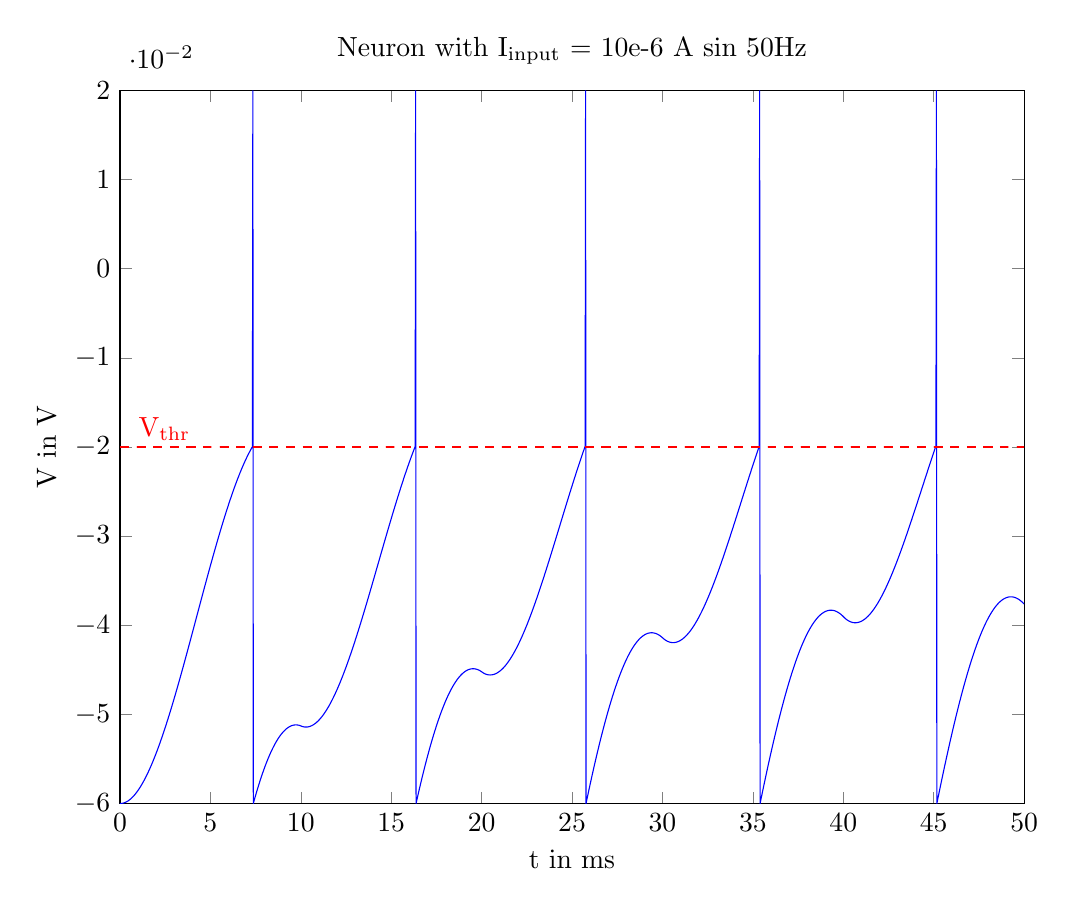
\begin{tikzpicture}

\begin{axis}[%
width=4.520833in,
height=3.565625in,
at={(0.758333in,0.48125in)},
scale only axis,
separate axis lines,
every outer x axis line/.append style={black},
every x tick label/.append style={font=\color{black}},
xmin=0,
xmax=50,
xlabel={t in ms},
every outer y axis line/.append style={black},
every y tick label/.append style={font=\color{black}},
ymin=-0.06,
ymax=0.02,
ylabel={V in V},
title={$\text{Neuron with I}_{\text{input}}\text{ = 10e-6 A sin 50Hz}$}
]
\addplot [color=blue,solid,forget plot]
  table[row sep=crcr]{%
0	-0.06\\
0.025	-0.06\\
0.05	-0.0599980365247778\\
0.075	-0.0599941146041379\\
0.1	-0.0599882393764192\\
0.125	-0.0599804160882086\\
0.15	-0.0599706500940483\\
0.175	-0.0599589468561358\\
0.2	-0.0599453119440173\\
0.225	-0.059929751034275\\
0.25	-0.0599122699102065\\
0.275	-0.059892874461499\\
0.3	-0.0598715706838958\\
0.325	-0.0598483646788564\\
0.35	-0.0598232626532105\\
0.375	-0.0597962709188047\\
0.4	-0.0597673958921432\\
0.425	-0.0597366440940218\\
0.45	-0.0597040221491551\\
0.475	-0.0596695367857978\\
0.5	-0.0596331948353591\\
0.525	-0.0595950032320107\\
0.55	-0.0595549690122884\\
0.575	-0.0595130993146878\\
0.6	-0.0594694013792528\\
0.625	-0.0594238825471583\\
0.65	-0.0593765502602863\\
0.675	-0.0593274120607965\\
0.7	-0.0592764755906892\\
0.725	-0.0592237485913633\\
0.75	-0.0591692389031676\\
0.775	-0.0591129544649457\\
0.8	-0.0590549033135751\\
0.825	-0.0589950935835\\
0.85	-0.058933533506258\\
0.875	-0.058870231410001\\
0.9	-0.0588051957190097\\
0.925	-0.0587384349532024\\
0.95	-0.0586699577276374\\
0.975	-0.0585997727520102\\
1	-0.0585278888301441\\
1.025	-0.058454314859475\\
1.05	-0.0583790598305309\\
1.075	-0.0583021328264051\\
1.1	-0.0582235430222234\\
1.125	-0.0581432996846065\\
1.15	-0.0580614121711256\\
1.175	-0.057977889929753\\
1.2	-0.0578927424983067\\
1.225	-0.0578059795038898\\
1.25	-0.0577176106623237\\
1.275	-0.0576276457775766\\
1.3	-0.0575360947411857\\
1.325	-0.057442967531674\\
1.35	-0.0573482742139626\\
1.375	-0.0572520249387764\\
1.4	-0.0571542299420451\\
1.425	-0.0570548995442988\\
1.45	-0.0569540441500579\\
1.475	-0.0568516742472188\\
1.5	-0.056747800406433\\
1.525	-0.056642433280482\\
1.55	-0.0565355836036469\\
1.575	-0.0564272621910727\\
1.6	-0.0563174799381273\\
1.625	-0.0562062478197566\\
1.65	-0.056093576889833\\
1.675	-0.0559794782805003\\
1.7	-0.0558639632015132\\
1.725	-0.0557470429395718\\
1.75	-0.0556287288576516\\
1.775	-0.0555090323943285\\
1.8	-0.0553879650630991\\
1.825	-0.0552655384516966\\
1.85	-0.0551417642214016\\
1.875	-0.0550166541063486\\
1.9	-0.0548902199128278\\
1.925	-0.0547624735185827\\
1.95	-0.0546334268721027\\
1.975	-0.0545030919919116\\
2	-0.0543714809658519\\
2.025	-0.0542386059503641\\
2.05	-0.0541044791697627\\
2.075	-0.0539691129155068\\
2.1	-0.0538325195454676\\
2.125	-0.0536947114831906\\
2.15	-0.0535557012171552\\
2.175	-0.0534155013000284\\
2.2	-0.053274124347916\\
2.225	-0.053131583039609\\
2.25	-0.0529878901158266\\
2.275	-0.0528430583784544\\
2.3	-0.0526971006897804\\
2.325	-0.052550029971725\\
2.35	-0.0524018592050695\\
2.375	-0.0522526014286794\\
2.4	-0.0521022697387245\\
2.425	-0.0519508772878955\\
2.45	-0.0517984372846171\\
2.475	-0.0516449629922575\\
2.5	-0.0514904677283342\\
2.525	-0.0513349648637167\\
2.55	-0.0511784678218261\\
2.575	-0.0510209900778307\\
2.6	-0.050862545157839\\
2.625	-0.0507031466380891\\
2.65	-0.0505428081441349\\
2.675	-0.05038154335003\\
2.7	-0.050219365977507\\
2.725	-0.0500562897951556\\
2.75	-0.0498923286175964\\
2.775	-0.0497274963046524\\
2.8	-0.0495618067605175\\
2.825	-0.0493952739329223\\
2.85	-0.0492279118122969\\
2.875	-0.0490597344309316\\
2.9	-0.0488907558621341\\
2.925	-0.0487209902193848\\
2.95	-0.0485504516554895\\
2.975	-0.048379154361729\\
3	-0.0482071125670071\\
3.025	-0.0480343405369959\\
3.05	-0.0478608525732782\\
3.075	-0.0476866630124887\\
3.1	-0.0475117862254523\\
3.125	-0.04733623661632\\
3.15	-0.0471600286217036\\
3.175	-0.0469831767098073\\
3.2	-0.046805695379558\\
3.225	-0.0466275991597336\\
3.25	-0.0464489026080889\\
3.275	-0.0462696203104802\\
3.3	-0.0460897668799877\\
3.325	-0.0459093569560367\\
3.35	-0.0457284052035166\\
3.375	-0.0455469263118983\\
3.4	-0.0453649349943503\\
3.425	-0.0451824459868535\\
3.45	-0.0449994740473136\\
3.475	-0.0448160339546731\\
3.5	-0.0446321405080216\\
3.525	-0.0444478085257045\\
3.55	-0.0442630528444307\\
3.575	-0.0440778883183795\\
3.6	-0.0438923298183055\\
3.625	-0.0437063922306432\\
3.65	-0.0435200904566103\\
3.675	-0.0433334394113099\\
3.7	-0.043146454022832\\
3.725	-0.0429591492313539\\
3.75	-0.0427715399882403\\
3.775	-0.0425836412551419\\
3.8	-0.042395468003094\\
3.825	-0.0422070352116142\\
3.85	-0.0420183578677994\\
3.875	-0.0418294509654224\\
3.9	-0.0416403295040282\\
3.925	-0.0414510084880296\\
3.95	-0.0412615029258025\\
3.975	-0.0410718278287811\\
4	-0.0408819982105527\\
4.025	-0.0406920290859526\\
4.05	-0.0405019354701579\\
4.075	-0.040311732377783\\
4.1	-0.0401214348219729\\
4.125	-0.0399310578134988\\
4.15	-0.0397406163598516\\
4.175	-0.0395501254643375\\
4.2	-0.0393596001251724\\
4.225	-0.0391690553345774\\
4.25	-0.0389785060778738\\
4.275	-0.0387879673325797\\
4.3	-0.0385974540675058\\
4.325	-0.0384069812418523\\
4.35	-0.0382165638043065\\
4.375	-0.0380262166921403\\
4.4	-0.0378359548303091\\
4.425	-0.0376457931305512\\
4.45	-0.0374557464904874\\
4.475	-0.0372658297927225\\
4.5	-0.0370760579039466\\
4.525	-0.0368864456740379\\
4.55	-0.0366970079351667\\
4.575	-0.0365077595008996\\
4.6	-0.0363187151653059\\
4.625	-0.036129889702064\\
4.65	-0.0359412978635701\\
4.675	-0.0357529543800474\\
4.7	-0.0355648739586568\\
4.725	-0.0353770712826094\\
4.75	-0.0351895610102797\\
4.775	-0.0350023577743207\\
4.8	-0.0348154761807808\\
4.825	-0.0346289308082218\\
4.85	-0.0344427362068386\\
4.875	-0.034256906897581\\
4.9	-0.0340714573712769\\
4.925	-0.0338864020877572\\
4.95	-0.0337017554749834\\
4.975	-0.0335175319281755\\
5	-0.0333337458089438\\
5.025	-0.0331504114444215\\
5.05	-0.0329675431263992\\
5.075	-0.0327851551104628\\
5.1	-0.0326032616151322\\
5.125	-0.0324218768210029\\
5.15	-0.0322410148698902\\
5.175	-0.032060689863975\\
5.2	-0.0318809158649524\\
5.225	-0.031701706893183\\
5.25	-0.031523076926846\\
5.275	-0.0313450399010956\\
5.3	-0.0311676097072196\\
5.325	-0.0309908001918008\\
5.35	-0.0308146251558808\\
5.375	-0.0306390983541273\\
5.4	-0.0304642334940033\\
5.425	-0.0302900442349397\\
5.45	-0.0301165441875108\\
5.475	-0.0299437469126129\\
5.5	-0.0297716659206453\\
5.525	-0.0296003146706949\\
5.55	-0.029429706569724\\
5.575	-0.029259854971761\\
5.6	-0.0290907731770942\\
5.625	-0.0289224744314693\\
5.65	-0.0287549719252898\\
5.675	-0.0285882787928212\\
5.7	-0.0284224081113979\\
5.725	-0.0282573729006347\\
5.75	-0.0280931861216407\\
5.775	-0.0279298606762372\\
5.8	-0.0277674094061794\\
5.825	-0.0276058450923818\\
5.85	-0.0274451804541466\\
5.875	-0.0272854281483968\\
5.9	-0.0271266007689124\\
5.925	-0.0269687108455709\\
5.95	-0.0268117708435914\\
5.975	-0.0266557931627828\\
6	-0.0265007901367961\\
6.025	-0.0263467740323803\\
6.05	-0.026193757048643\\
6.075	-0.0260417513163145\\
6.1	-0.0258907688970167\\
6.125	-0.0257408217825356\\
6.15	-0.0255919218940986\\
6.175	-0.0254440810816559\\
6.2	-0.025297311123166\\
6.225	-0.025151623723886\\
6.25	-0.0250070305156663\\
6.275	-0.0248635430562493\\
6.3	-0.0247211728285734\\
6.325	-0.024579931240081\\
6.35	-0.0244398296220311\\
6.375	-0.0243008792288172\\
6.4	-0.0241630912372889\\
6.425	-0.0240264767460792\\
6.45	-0.0238910467749359\\
6.475	-0.0237568122640584\\
6.5	-0.0236237840734387\\
6.525	-0.0234919729822081\\
6.55	-0.0233613896879877\\
6.575	-0.0232320448062456\\
6.6	-0.0231039488696572\\
6.625	-0.0229771123274721\\
6.65	-0.0228515455448852\\
6.675	-0.0227272588024134\\
6.7	-0.0226042622952774\\
6.725	-0.0224825661327882\\
6.75	-0.0223621803377399\\
6.775	-0.0222431148458071\\
6.8	-0.0221253795049472\\
6.825	-0.0220089840748093\\
6.85	-0.0218939382261475\\
6.875	-0.0217802515402401\\
6.9	-0.0216679335083139\\
6.925	-0.0215569935309744\\
6.95	-0.0214474409176418\\
6.975	-0.0213392848859914\\
7	-0.0212325345614013\\
7.025	-0.021127198976404\\
7.05	-0.0210232870701455\\
7.075	-0.0209208076878484\\
7.1	-0.0208197695802819\\
7.125	-0.0207201814032372\\
7.15	-0.0206220517170089\\
7.175	-0.0205253889858818\\
7.2	-0.0204302015776241\\
7.225	-0.0203364977629861\\
7.25	-0.0202442857152053\\
7.275	-0.0201535735095173\\
7.3	-0.0200643691226722\\
7.325	-0.0199766804324579\\
7.35	0.02\\
7.375	-0.06\\
7.4	-0.0598164193726411\\
7.425	-0.0596346361673541\\
7.45	-0.0594546571321386\\
7.475	-0.0592764889148675\\
7.5	-0.059100138062849\\
7.525	-0.0589256110223952\\
7.55	-0.0587529141383965\\
7.575	-0.0585820536539025\\
7.6	-0.0584130357097091\\
7.625	-0.0582458663439527\\
7.65	-0.0580805514917095\\
7.675	-0.0579170969846028\\
7.7	-0.0577555085504152\\
7.725	-0.0575957918127082\\
7.75	-0.0574379522904485\\
7.775	-0.0572819953976398\\
7.8	-0.0571279264429623\\
7.825	-0.0569757506294177\\
7.85	-0.0568254730539818\\
7.875	-0.0566770987072629\\
7.9	-0.0565306324731673\\
7.925	-0.0563860791285712\\
7.95	-0.0562434433429992\\
7.975	-0.0561027296783103\\
8	-0.055963942588389\\
8.025	-0.0558270864188449\\
8.05	-0.0556921654067178\\
8.075	-0.0555591836801902\\
8.1	-0.0554281452583062\\
8.125	-0.0552990540506974\\
8.15	-0.0551719138573157\\
8.175	-0.0550467283681729\\
8.2	-0.0549235011630867\\
8.225	-0.0548022357114342\\
8.25	-0.0546829353719121\\
8.275	-0.0545656033923033\\
8.3	-0.0544502429092513\\
8.325	-0.0543368569480406\\
8.35	-0.0542254484223846\\
8.375	-0.0541160201342206\\
8.4	-0.0540085747735108\\
8.425	-0.0539031149180516\\
8.45	-0.0537996430332888\\
8.475	-0.0536981614721404\\
8.5	-0.0535986724748262\\
8.525	-0.0535011781687043\\
8.55	-0.0534056805681147\\
8.575	-0.0533121815742304\\
8.6	-0.0532206829749148\\
8.625	-0.0531311864445862\\
8.65	-0.0530436935440904\\
8.675	-0.0529582057205789\\
8.7	-0.0528747243073952\\
8.725	-0.0527932505239681\\
8.75	-0.0527137854757111\\
8.775	-0.0526363301539305\\
8.8	-0.0525608854357394\\
8.825	-0.0524874520839789\\
8.85	-0.052416030747147\\
8.875	-0.0523466219593343\\
8.9	-0.0522792261401666\\
8.925	-0.0522138435947549\\
8.95	-0.0521504745136524\\
8.975	-0.0520891189728187\\
9	-0.0520297769335912\\
9.025	-0.0519724482426635\\
9.05	-0.0519171326320707\\
9.075	-0.0518638297191825\\
9.1	-0.0518125390067026\\
9.125	-0.051763259882676\\
9.15	-0.0517159916205031\\
9.175	-0.0516707333789605\\
9.2	-0.0516274842022298\\
9.225	-0.051586243019933\\
9.25	-0.0515470086471749\\
9.275	-0.051509779784593\\
9.3	-0.0514745550184143\\
9.325	-0.0514413328205191\\
9.35	-0.0514101115485125\\
9.375	-0.051380889445802\\
9.4	-0.0513536646416835\\
9.425	-0.0513284351514329\\
9.45	-0.051305198876406\\
9.475	-0.0512839536041451\\
9.5	-0.0512646970084925\\
9.525	-0.0512474266497113\\
9.55	-0.0512321399746127\\
9.575	-0.0512188343166918\\
9.6	-0.0512075068962685\\
9.625	-0.0511981548206367\\
9.65	-0.0511907750842207\\
9.675	-0.0511853645687373\\
9.7	-0.0511819200433667\\
9.725	-0.0511804381649287\\
9.75	-0.0511809154780669\\
9.775	-0.0511833484154398\\
9.8	-0.0511877332979184\\
9.825	-0.0511940663347912\\
9.85	-0.0512023436239762\\
9.875	-0.0512125611522388\\
9.9	-0.0512247147954184\\
9.925	-0.0512388003186604\\
9.95	-0.0512548133766553\\
9.975	-0.0512727495138857\\
10	-0.0512926041648788\\
10.025	-0.0513143726544666\\
10.05	-0.0513341232476083\\
10.075	-0.0513518611101613\\
10.1	-0.0513675915161775\\
10.125	-0.0513813198476175\\
10.15	-0.0513930515940587\\
10.175	-0.0514027923523962\\
10.2	-0.051410547826537\\
10.225	-0.0514163238270884\\
10.25	-0.0514201262710379\\
10.275	-0.0514219611814283\\
10.3	-0.0514218346870253\\
10.325	-0.0514197530219781\\
10.35	-0.0514157225254744\\
10.375	-0.0514097496413879\\
10.4	-0.05140184091792\\
10.425	-0.0513920030072341\\
10.45	-0.0513802426650844\\
10.475	-0.0513665667504373\\
10.5	-0.0513509822250869\\
10.525	-0.0513334961532642\\
10.55	-0.0513141157012388\\
10.575	-0.0512928481369158\\
10.6	-0.0512697008294253\\
10.625	-0.0512446812487053\\
10.65	-0.0512177969650795\\
10.675	-0.0511890556488276\\
10.7	-0.0511584650697502\\
10.725	-0.0511260330967267\\
10.75	-0.0510917676972676\\
10.775	-0.0510556769370605\\
10.8	-0.0510177689795096\\
10.825	-0.0509780520852696\\
10.85	-0.0509365346117732\\
10.875	-0.0508932250127524\\
10.9	-0.0508481318377543\\
10.925	-0.0508012637316501\\
10.95	-0.050752629434139\\
10.975	-0.0507022377792456\\
11	-0.0506500976948113\\
11.025	-0.0505962182019806\\
11.05	-0.0505406084146802\\
11.075	-0.050483277539094\\
11.1	-0.0504242348731306\\
11.125	-0.0503634898058865\\
11.15	-0.0503010518171024\\
11.175	-0.0502369304766148\\
11.2	-0.0501711354438013\\
11.225	-0.0501036764670207\\
11.25	-0.0500345633830468\\
11.275	-0.0499638061164979\\
11.3	-0.0498914146792596\\
11.325	-0.0498173991699028\\
11.35	-0.0497417697730958\\
11.375	-0.0496645367590118\\
11.4	-0.0495857104827299\\
11.425	-0.0495053013836318\\
11.45	-0.0494233199847927\\
11.475	-0.0493397768923667\\
11.5	-0.049254682794968\\
11.525	-0.0491680484630457\\
11.55	-0.0490798847482542\\
11.575	-0.0489902025828184\\
11.6	-0.0488990129788937\\
11.625	-0.0488063270279211\\
11.65	-0.048712155899977\\
11.675	-0.048616510843119\\
11.7	-0.0485194031827254\\
11.725	-0.048420844320831\\
11.75	-0.0483208457354576\\
11.775	-0.04821941897994\\
11.8	-0.0481165756822466\\
11.825	-0.0480123275442962\\
11.85	-0.0479066863412697\\
11.875	-0.047799663920917\\
11.9	-0.0476912722028598\\
11.925	-0.0475815231778896\\
11.95	-0.0474704289072613\\
11.975	-0.0473580015219823\\
12	-0.0472442532220974\\
12.025	-0.0471291962759691\\
12.05	-0.0470128430195536\\
12.075	-0.0468952058556733\\
12.1	-0.0467762972532836\\
12.125	-0.0466561297467371\\
12.15	-0.0465347159350428\\
12.175	-0.0464120684811213\\
12.2	-0.0462882001110562\\
12.225	-0.0461631236133413\\
12.25	-0.0460368518381245\\
12.275	-0.0459093976964467\\
12.3	-0.0457807741594776\\
12.325	-0.045650994257748\\
12.35	-0.0455200710803775\\
12.375	-0.0453880177742991\\
12.4	-0.0452548475434801\\
12.425	-0.0451205736481393\\
12.45	-0.0449852094039603\\
12.475	-0.0448487681813023\\
12.5	-0.0447112634044064\\
12.525	-0.0445727085505987\\
12.55	-0.0444331171494909\\
12.575	-0.0442925027821764\\
12.6	-0.0441508790804238\\
12.625	-0.0440082597258674\\
12.65	-0.0438646584491938\\
12.675	-0.0437200890293262\\
12.7	-0.043574565292605\\
12.725	-0.0434281011119658\\
12.75	-0.0432807104061146\\
12.775	-0.0431324071386993\\
12.8	-0.0429832053174793\\
12.825	-0.0428331189934917\\
12.85	-0.0426821622602149\\
12.875	-0.0425303492527298\\
12.9	-0.0423776941468778\\
12.925	-0.0422242111584166\\
12.95	-0.0420699145421737\\
12.975	-0.0419148185911965\\
13	-0.041758937635901\\
13.025	-0.0416022860432175\\
13.05	-0.0414448782157343\\
13.075	-0.0412867285908387\\
13.1	-0.0411278516398564\\
13.125	-0.0409682618671881\\
13.15	-0.0408079738094445\\
13.175	-0.0406470020345788\\
13.2	-0.0404853611410176\\
13.225	-0.0403230657567896\\
13.25	-0.0401601305386522\\
13.275	-0.0399965701712171\\
13.3	-0.0398323993660728\\
13.325	-0.0396676328609066\\
13.35	-0.0395022854186243\\
13.375	-0.0393363718264682\\
13.4	-0.0391699068951338\\
13.425	-0.039002905457885\\
13.45	-0.0388353823696675\\
13.475	-0.0386673525062212\\
13.5	-0.0384988307631908\\
13.525	-0.0383298320552357\\
13.55	-0.0381603713151382\\
13.575	-0.0379904634929102\\
13.6	-0.0378201235548998\\
13.625	-0.0376493664828961\\
13.65	-0.0374782072732325\\
13.675	-0.0373066609358906\\
13.7	-0.0371347424936012\\
13.725	-0.0369624669809462\\
13.75	-0.0367898494434586\\
13.775	-0.0366169049367221\\
13.8	-0.0364436485254703\\
13.825	-0.0362700952826846\\
13.85	-0.0360962602886921\\
13.875	-0.0359221586302629\\
13.9	-0.0357478053997066\\
13.925	-0.0355732156939688\\
13.95	-0.0353984046137268\\
13.975	-0.0352233872624856\\
14	-0.035048178745673\\
14.025	-0.0348727941697351\\
14.05	-0.034697248641231\\
14.075	-0.0345215572659283\\
14.1	-0.0343457351478979\\
14.125	-0.0341697973886089\\
14.15	-0.033993759086024\\
14.175	-0.0338176353336945\\
14.2	-0.033641441219856\\
14.225	-0.0334651918265242\\
14.25	-0.0332889022285908\\
14.275	-0.0331125874929199\\
14.3	-0.0329362626774451\\
14.325	-0.0327599428302668\\
14.35	-0.0325836429887499\\
14.375	-0.0324073781786226\\
14.4	-0.0322311634130753\\
14.425	-0.0320550136918604\\
14.45	-0.0318789440003934\\
14.475	-0.0317029693088537\\
14.5	-0.0315271045712874\\
14.525	-0.0313513647247104\\
14.55	-0.0311757646882125\\
14.575	-0.0310003193620629\\
14.6	-0.0308250436268162\\
14.625	-0.0306499523424205\\
14.65	-0.0304750603473258\\
14.675	-0.0303003824575936\\
14.7	-0.0301259334660092\\
14.725	-0.0299517281411934\\
14.75	-0.0297777812267172\\
14.775	-0.0296041074402171\\
14.8	-0.0294307214725125\\
14.825	-0.0292576379867242\\
14.85	-0.0290848716173947\\
14.875	-0.0289124369696108\\
14.9	-0.0287403486181266\\
14.925	-0.0285686211064898\\
14.95	-0.0283972689461691\\
14.975	-0.0282263066156832\\
15	-0.0280557485597328\\
15.025	-0.0278856091883335\\
15.05	-0.0277159028759515\\
15.075	-0.0275466439606412\\
15.1	-0.0273778467431851\\
15.125	-0.0272095254862357\\
15.15	-0.0270416944134599\\
15.175	-0.0268743677086858\\
15.2	-0.0267075595150514\\
15.225	-0.0265412839341567\\
15.25	-0.0263755550252173\\
15.275	-0.0262103868042209\\
15.3	-0.0260457932430872\\
15.325	-0.0258817882688287\\
15.35	-0.0257183857627162\\
15.375	-0.0255555995594456\\
15.4	-0.0253934434463082\\
15.425	-0.0252319311623638\\
15.45	-0.0250710763976164\\
15.475	-0.0249108927921933\\
15.5	-0.0247513939355266\\
15.525	-0.024592593365539\\
15.55	-0.0244345045678311\\
15.575	-0.0242771409748728\\
15.6	-0.0241205159651982\\
15.625	-0.0239646428626031\\
15.65	-0.0238095349353458\\
15.675	-0.023655205395352\\
15.7	-0.0235016673974224\\
15.725	-0.0233489340384441\\
15.75	-0.0231970183566056\\
15.775	-0.0230459333306146\\
15.8	-0.022895691878921\\
15.825	-0.0227463068589415\\
15.85	-0.0225977910662899\\
15.875	-0.0224501572340097\\
15.9	-0.0223034180318113\\
15.925	-0.0221575860653125\\
15.95	-0.0220126738752837\\
15.975	-0.0218686939368959\\
16	-0.0217256586589739\\
16.025	-0.0215835803832527\\
16.05	-0.0214424713836382\\
16.075	-0.0213023438654722\\
16.1	-0.0211632099648015\\
16.125	-0.0210250817476509\\
16.15	-0.0208879712093011\\
16.175	-0.0207518902735704\\
16.2	-0.0206168507921007\\
16.225	-0.0204828645436484\\
16.25	-0.0203499432333793\\
16.275	-0.020218098492168\\
16.3	-0.0200873418759023\\
16.325	-0.0199576848647916\\
16.35	0.02\\
16.375	-0.06\\
16.4	-0.0597729642065437\\
16.425	-0.0595473250329109\\
16.45	-0.0593230929410505\\
16.475	-0.0591002783147577\\
16.5	-0.0588788914590113\\
16.525	-0.0586589425993167\\
16.55	-0.0584404418810536\\
16.575	-0.0582233993688288\\
16.6	-0.0580078250458339\\
16.625	-0.0577937288132084\\
16.65	-0.0575811204894072\\
16.675	-0.0573700098095741\\
16.7	-0.0571604064249201\\
16.725	-0.0569523199021069\\
16.75	-0.0567457597226353\\
16.775	-0.0565407352822402\\
16.8	-0.0563372558902892\\
16.825	-0.056135330769188\\
16.85	-0.0559349690537903\\
16.875	-0.0557361797908138\\
16.9	-0.0555389719382611\\
16.925	-0.0553433543648468\\
16.95	-0.0551493358494295\\
16.975	-0.0549569250804496\\
17	-0.0547661306553733\\
17.025	-0.0545769610801412\\
17.05	-0.0543894247686233\\
17.075	-0.0542035300420799\\
17.1	-0.0540192851286279\\
17.125	-0.0538366981627124\\
17.15	-0.0536557771845854\\
17.175	-0.0534765301397894\\
17.2	-0.0532989648786468\\
17.225	-0.0531230891557563\\
17.25	-0.0529489106294936\\
17.275	-0.0527764368615199\\
17.3	-0.0526056753162948\\
17.325	-0.0524366333605964\\
17.35	-0.052269318263047\\
17.375	-0.0521037371936448\\
17.4	-0.0519398972233017\\
17.425	-0.0517778053233881\\
17.45	-0.0516174683652825\\
17.475	-0.0514588931199285\\
17.5	-0.0513020862573974\\
17.525	-0.0511470543464573\\
17.55	-0.0509938038541484\\
17.575	-0.050842341145365\\
17.6	-0.050692672482443\\
17.625	-0.0505448040247547\\
17.65	-0.0503987418283096\\
17.675	-0.0502544918453613\\
17.7	-0.0501120599240218\\
17.725	-0.0499714518078808\\
17.75	-0.0498326731356332\\
17.775	-0.0496957294407115\\
17.8	-0.0495606261509263\\
17.825	-0.0494273685881118\\
17.85	-0.0492959619677792\\
17.875	-0.0491664113987758\\
17.9	-0.0490387218829514\\
17.925	-0.0489128983148308\\
17.95	-0.0487889454812932\\
17.975	-0.0486668680612585\\
18	-0.0485466706253799\\
18.025	-0.0484283576357433\\
18.05	-0.048311933445574\\
18.075	-0.0481974022989492\\
18.1	-0.0480847683305183\\
18.125	-0.047974035565229\\
18.15	-0.047865207918061\\
18.175	-0.0477582891937663\\
18.2	-0.0476532830866161\\
18.225	-0.0475501931801548\\
18.25	-0.0474490229469609\\
18.275	-0.0473497757484145\\
18.3	-0.0472524548344722\\
18.325	-0.0471570633434484\\
18.35	-0.047063604301804\\
18.375	-0.0469720806239414\\
18.4	-0.0468824951120073\\
18.425	-0.0467948504557018\\
18.45	-0.0467091492320949\\
18.475	-0.0466253939054495\\
18.5	-0.0465435868270521\\
18.525	-0.0464637302350495\\
18.55	-0.0463858262542941\\
18.575	-0.0463098768961944\\
18.6	-0.0462358840585738\\
18.625	-0.0461638495255361\\
18.65	-0.0460937749673379\\
18.675	-0.0460256619402683\\
18.7	-0.0459595118865354\\
18.725	-0.0458953261341604\\
18.75	-0.045833105896878\\
18.775	-0.0457728522740445\\
18.8	-0.0457145662505531\\
18.825	-0.0456582486967555\\
18.85	-0.0456039003683917\\
18.875	-0.0455515219065259\\
18.9	-0.0455011138374902\\
18.925	-0.0454526765728352\\
18.95	-0.0454062104092875\\
18.975	-0.0453617155287147\\
19	-0.0453191919980975\\
19.025	-0.0452786397695085\\
19.05	-0.0452400586800987\\
19.075	-0.0452034484520903\\
19.1	-0.0451688086927782\\
19.125	-0.0451361388945364\\
19.15	-0.0451054384348338\\
19.175	-0.0450767065762554\\
19.2	-0.0450499424665315\\
19.225	-0.0450251451385739\\
19.25	-0.0450023135105192\\
19.275	-0.044981446385779\\
19.3	-0.0449625424530972\\
19.325	-0.0449456002866154\\
19.35	-0.0449306183459435\\
19.375	-0.0449175949762395\\
19.4	-0.0449065284082949\\
19.425	-0.0448974167586277\\
19.45	-0.0448902580295829\\
19.475	-0.044885050109439\\
19.5	-0.0448817907725232\\
19.525	-0.0448804776793319\\
19.55	-0.0448811083766593\\
19.575	-0.0448836802977333\\
19.6	-0.0448881907623573\\
19.625	-0.0448946369770603\\
19.65	-0.0449030160352532\\
19.675	-0.0449133249173923\\
19.7	-0.0449255604911501\\
19.725	-0.0449397195115926\\
19.75	-0.0449557986213641\\
19.775	-0.0449737943508787\\
19.8	-0.0449937031185187\\
19.825	-0.0450155212308401\\
19.85	-0.0450392448827849\\
19.875	-0.0450648701579005\\
19.9	-0.045092393028566\\
19.925	-0.0451218093562251\\
19.95	-0.0451531148916261\\
19.975	-0.0451863052750691\\
20	-0.0452213760366592\\
20.025	-0.0452583225965676\\
20.05	-0.045293213314854\\
20.075	-0.0453260534522389\\
20.1	-0.0453568483773999\\
20.125	-0.0453856035666869\\
20.15	-0.0454123246038304\\
20.175	-0.0454370171796434\\
20.2	-0.0454596870917162\\
20.225	-0.0454803402441046\\
20.25	-0.0454989826470115\\
20.275	-0.045515620416462\\
20.3	-0.0455302597739714\\
20.325	-0.0455429070462068\\
20.35	-0.0455535686646425\\
20.375	-0.0455622511652082\\
20.4	-0.0455689611879307\\
20.425	-0.0455737054765698\\
20.45	-0.0455764908782467\\
20.475	-0.0455773243430667\\
20.5	-0.0455762129237348\\
20.525	-0.0455731637751654\\
20.55	-0.0455681841540853\\
20.575	-0.0455612814186302\\
20.6	-0.0455524630279354\\
20.625	-0.0455417365417191\\
20.65	-0.0455291096198608\\
20.675	-0.045514590021972\\
20.7	-0.0454981856069617\\
20.725	-0.0454799043325952\\
20.75	-0.0454597542550464\\
20.775	-0.0454377435284448\\
20.8	-0.0454138804044154\\
20.825	-0.0453881732316132\\
20.85	-0.0453606304552509\\
20.875	-0.0453312606166214\\
20.9	-0.0453000723526136\\
20.925	-0.0452670743952223\\
20.95	-0.0452322755710523\\
20.975	-0.0451956848008166\\
21	-0.0451573110988284\\
21.025	-0.0451171635724876\\
21.05	-0.045075251421761\\
21.075	-0.045031583938657\\
21.1	-0.0449861705066947\\
21.125	-0.0449390206003667\\
21.15	-0.0448901437845964\\
21.175	-0.0448395497141901\\
21.2	-0.0447872481332827\\
21.225	-0.0447332488747783\\
21.25	-0.0446775618597851\\
21.275	-0.0446201970970443\\
21.3	-0.0445611646823547\\
21.325	-0.0445004747979901\\
21.35	-0.0444381377121129\\
21.375	-0.0443741637781814\\
21.4	-0.0443085634343516\\
21.425	-0.0442413472028744\\
21.45	-0.0441725256894871\\
21.475	-0.0441021095827994\\
21.5	-0.0440301096536746\\
21.525	-0.0439565367546056\\
21.55	-0.0438814018190852\\
21.575	-0.0438047158609723\\
21.6	-0.0437264899738523\\
21.625	-0.0436467353303922\\
21.65	-0.043565463181692\\
21.675	-0.0434826848566297\\
21.7	-0.0433984117612022\\
21.725	-0.0433126553778616\\
21.75	-0.0432254272648457\\
21.775	-0.0431367390555046\\
21.8	-0.0430466024576223\\
21.825	-0.0429550292527335\\
21.85	-0.0428620312954359\\
21.875	-0.0427676205126978\\
21.9	-0.0426718089031611\\
21.925	-0.0425746085364402\\
21.95	-0.0424760315524155\\
21.975	-0.0423760901605237\\
22	-0.0422747966390424\\
22.025	-0.0421721633343717\\
22.05	-0.0420682026603102\\
22.075	-0.041962927097328\\
22.1	-0.0418563491918342\\
22.125	-0.0417484815554413\\
22.15	-0.0416393368642253\\
22.175	-0.0415289278579808\\
22.2	-0.0414172673394735\\
22.225	-0.0413043681736876\\
22.25	-0.04119024328707\\
22.275	-0.0410749056667697\\
22.3	-0.0409583683598749\\
22.325	-0.0408406444726443\\
22.35	-0.0407217471697365\\
22.375	-0.0406016896734347\\
22.4	-0.0404804852628679\\
22.425	-0.0403581472732286\\
22.45	-0.0402346890949869\\
22.475	-0.0401101241731013\\
22.5	-0.0399844660062259\\
22.525	-0.0398577281459137\\
22.55	-0.0397299241958176\\
22.575	-0.0396010678108872\\
22.6	-0.0394711726965629\\
22.625	-0.0393402526079661\\
22.65	-0.0392083213490873\\
22.675	-0.0390753927719699\\
22.7	-0.0389414807758921\\
22.725	-0.0388065993065448\\
22.75	-0.0386707623552071\\
22.775	-0.0385339839579191\\
22.8	-0.038396278194651\\
22.825	-0.0382576591884704\\
22.85	-0.0381181411047062\\
22.875	-0.0379777381501098\\
22.9	-0.0378364645720144\\
22.925	-0.0376943346574904\\
22.95	-0.0375513627324998\\
22.975	-0.0374075631610468\\
23	-0.0372629503443267\\
23.025	-0.0371175387198721\\
23.05	-0.0369713427606972\\
23.075	-0.0368243769744392\\
23.1	-0.0366766559024979\\
23.125	-0.036528194119173\\
23.15	-0.0363790062307995\\
23.175	-0.0362291068748804\\
23.2	-0.0360785107192185\\
23.225	-0.0359272324610449\\
23.25	-0.0357752868261469\\
23.275	-0.035622688567993\\
23.3	-0.0354694524668568\\
23.325	-0.0353155933289386\\
23.35	-0.0351611259854863\\
23.375	-0.035006065291913\\
23.4	-0.034850426126915\\
23.425	-0.0346942233915868\\
23.45	-0.034537472008535\\
23.475	-0.0343801869209915\\
23.5	-0.0342223830919242\\
23.525	-0.0340640755031473\\
23.55	-0.0339052791544299\\
23.575	-0.0337460090626037\\
23.6	-0.0335862802606691\\
23.625	-0.0334261077969009\\
23.65	-0.0332655067339524\\
23.675	-0.0331044921479587\\
23.7	-0.0329430791276391\\
23.725	-0.032781282773399\\
23.75	-0.0326191181964303\\
23.775	-0.0324566005178114\\
23.8	-0.0322937448676068\\
23.825	-0.0321305663839657\\
23.85	-0.0319670802122201\\
23.875	-0.031803301503982\\
23.9	-0.0316392454162415\\
23.925	-0.0314749271104623\\
23.95	-0.0313103617516791\\
23.975	-0.031145564507593\\
24	-0.0309805505476677\\
24.025	-0.0308153350422247\\
24.05	-0.0306499331615394\\
24.075	-0.030484360074936\\
24.1	-0.030318630949883\\
24.125	-0.0301527609510891\\
24.15	-0.029986765239598\\
24.175	-0.0298206589718845\\
24.2	-0.0296544572989506\\
24.225	-0.029488175365421\\
24.25	-0.0293218283086403\\
24.275	-0.0291554312577693\\
24.3	-0.0289889993328824\\
24.325	-0.0288225476440655\\
24.35	-0.0286560912905142\\
24.375	-0.0284896453596325\\
24.4	-0.0283232249261326\\
24.425	-0.0281568450511351\\
24.45	-0.0279905207812698\\
24.475	-0.027824267147778\\
24.5	-0.0276580991656144\\
24.525	-0.0274920318325516\\
24.55	-0.0273260801282841\\
24.575	-0.0271602590135342\\
24.6	-0.0269945834291589\\
24.625	-0.0268290682952574\\
24.65	-0.0266637285102805\\
24.675	-0.026498578950141\\
24.7	-0.0263336344673252\\
24.725	-0.0261689098900061\\
24.75	-0.0260044200211579\\
24.775	-0.0258401796376717\\
24.8	-0.0256762034894735\\
24.825	-0.0255125062986427\\
24.85	-0.0253491027585335\\
24.875	-0.0251860075328967\\
24.9	-0.0250232352550042\\
24.925	-0.0248608005267753\\
24.95	-0.0246987179179038\\
24.975	-0.0245370019649887\\
25	-0.024375667170665\\
25.025	-0.0242147280027383\\
25.05	-0.0240541988933203\\
25.075	-0.0238940942379666\\
25.1	-0.0237344283948172\\
25.125	-0.0235752156837387\\
25.15	-0.0234164703854692\\
25.175	-0.023258206740765\\
25.2	-0.0231004389495505\\
25.225	-0.0229431811700695\\
25.25	-0.0227864475180403\\
25.275	-0.0226302520658119\\
25.3	-0.0224746088415241\\
25.325	-0.0223195318282695\\
25.35	-0.0221650349632584\\
25.375	-0.0220111321369865\\
25.4	-0.0218578371924053\\
25.425	-0.0217051639240957\\
25.45	-0.0215531260774439\\
25.475	-0.0214017373478212\\
25.5	-0.0212510113797655\\
25.525	-0.0211009617661673\\
25.55	-0.0209516020474578\\
25.575	-0.0208029457108004\\
25.6	-0.020655006189286\\
25.625	-0.0205077968611307\\
25.65	-0.020361331048877\\
25.675	-0.0202156220185994\\
25.7	-0.0200706829791117\\
25.725	-0.0199265270811792\\
25.75	0.02\\
25.775	-0.06\\
25.8	-0.0597573733816329\\
25.825	-0.0595158341578966\\
25.85	-0.0592753945469977\\
25.875	-0.0590360667060157\\
25.9	-0.0587978627301373\\
25.925	-0.0585607946518927\\
25.95	-0.0583248744403974\\
25.975	-0.0580901140005968\\
26	-0.0578565251725155\\
26.025	-0.0576241197305105\\
26.05	-0.0573929093825278\\
26.075	-0.0571629057693646\\
26.1	-0.0569341204639342\\
26.125	-0.0567065649705358\\
26.15	-0.0564802507241288\\
26.175	-0.056255189089611\\
26.2	-0.0560313913611012\\
26.225	-0.0558088687612264\\
26.25	-0.0555876324404133\\
26.275	-0.0553676934761844\\
26.3	-0.0551490628724587\\
26.325	-0.0549317515588566\\
26.35	-0.0547157703900098\\
26.375	-0.0545011301448759\\
26.4	-0.0542878415260574\\
26.425	-0.0540759151591258\\
26.45	-0.0538653615919499\\
26.475	-0.0536561912940299\\
26.5	-0.0534484146558353\\
26.525	-0.0532420419881486\\
26.55	-0.0530370835214134\\
26.575	-0.0528335494050877\\
26.6	-0.0526314497070022\\
26.625	-0.0524307944127238\\
26.65	-0.0522315934249237\\
26.675	-0.0520338565627519\\
26.7	-0.051837593561215\\
26.725	-0.0516428140705609\\
26.75	-0.0514495276556683\\
26.775	-0.0512577437954406\\
26.8	-0.0510674718822066\\
26.825	-0.0508787212211256\\
26.85	-0.050691501029598\\
26.875	-0.050505820436682\\
26.9	-0.0503216884825146\\
26.925	-0.0501391141177397\\
26.95	-0.0499581062029401\\
26.975	-0.0497786735080765\\
27	-0.0496008247119311\\
27.025	-0.0494245684015576\\
27.05	-0.0492499130717362\\
27.075	-0.049076867124435\\
27.1	-0.0489054388682771\\
27.125	-0.0487356365180125\\
27.15	-0.0485674681939973\\
27.175	-0.0484009419216777\\
27.2	-0.0482360656310804\\
27.225	-0.0480728471563088\\
27.25	-0.0479112942350447\\
27.275	-0.0477514145080571\\
27.3	-0.0475932155187157\\
27.325	-0.0474367047125113\\
27.35	-0.0472818894365821\\
27.375	-0.047128776939246\\
27.4	-0.0469773743695389\\
27.425	-0.0468276887767597\\
27.45	-0.0466797271100207\\
27.475	-0.0465334962178049\\
27.5	-0.0463890028475291\\
27.525	-0.0462462536451136\\
27.55	-0.0461052551545581\\
27.575	-0.0459660138175236\\
27.6	-0.0458285359729212\\
27.625	-0.0456928278565067\\
27.65	-0.0455588956004822\\
27.675	-0.0454267452331036\\
27.7	-0.0452963826782947\\
27.725	-0.045167813755268\\
27.75	-0.0450410441781519\\
27.775	-0.044916079555624\\
27.8	-0.0447929253905515\\
27.825	-0.0446715870796379\\
27.85	-0.0445520699130765\\
27.875	-0.0444343790742099\\
27.9	-0.0443185196391969\\
27.925	-0.0442044965766857\\
27.95	-0.0440923147474935\\
27.975	-0.0439819789042932\\
28	-0.043873493691307\\
28.025	-0.0437668636440056\\
28.05	-0.0436620931888156\\
28.075	-0.0435591866428328\\
28.1	-0.0434581482135421\\
28.125	-0.0433589819985453\\
28.15	-0.043261691985294\\
28.175	-0.0431662820508312\\
28.2	-0.0430727559615384\\
28.225	-0.0429811173728898\\
28.25	-0.042891369829214\\
28.275	-0.042803516763462\\
28.3	-0.0427175614969821\\
28.325	-0.042633507239302\\
28.35	-0.0425513570879179\\
28.375	-0.04247111402809\\
28.4	-0.0423927809326456\\
28.425	-0.0423163605617885\\
28.45	-0.0422418555629164\\
28.475	-0.042169268470444\\
28.5	-0.042098601705634\\
28.525	-0.042029857576435\\
28.55	-0.0419630382773261\\
28.575	-0.0418981458891689\\
28.6	-0.0418351823790658\\
28.625	-0.0417741496002269\\
28.65	-0.041715049291842\\
28.675	-0.0416578830789611\\
28.7	-0.0416026524723815\\
28.725	-0.0415493588685419\\
28.75	-0.0414980035494235\\
28.775	-0.0414485876824586\\
28.8	-0.0414011123204462\\
28.825	-0.0413555784014739\\
28.85	-0.0413119867488483\\
28.875	-0.0412703380710313\\
28.9	-0.0412306329615844\\
28.925	-0.0411928718991191\\
28.95	-0.0411570552472557\\
28.975	-0.041123183254588\\
29	-0.0410912560546561\\
29.025	-0.0410612736659257\\
29.05	-0.0410332359917748\\
29.075	-0.0410071428204873\\
29.1	-0.0409829938252541\\
29.125	-0.0409607885641812\\
29.15	-0.0409405264803045\\
29.175	-0.0409222069016124\\
29.2	-0.0409058290410751\\
29.225	-0.0408913919966812\\
29.25	-0.0408788947514812\\
29.275	-0.0408683361736385\\
29.3	-0.0408597150164872\\
29.325	-0.0408530299185968\\
29.35	-0.040848279403845\\
29.375	-0.0408454618814962\\
29.4	-0.0408445756462885\\
29.425	-0.0408456188785263\\
29.45	-0.0408485896441817\\
29.475	-0.0408534858950014\\
29.5	-0.0408603054686217\\
29.525	-0.0408690460886901\\
29.55	-0.0408797053649941\\
29.575	-0.0408922807935972\\
29.6	-0.0409067697569816\\
29.625	-0.0409231695241981\\
29.65	-0.0409414772510231\\
29.675	-0.0409616899801228\\
29.7	-0.0409838046412237\\
29.725	-0.041007818051291\\
29.75	-0.0410337269147133\\
29.775	-0.0410615278234946\\
29.8	-0.0410912172574531\\
29.825	-0.0411227915844271\\
29.85	-0.0411562470604879\\
29.875	-0.0411915798301593\\
29.9	-0.0412287859266441\\
29.925	-0.041267861272058\\
29.95	-0.0413088016776694\\
29.975	-0.0413516028441473\\
30	-0.0413962603618147\\
30.025	-0.0414427697109102\\
30.05	-0.0414871993114107\\
30.075	-0.0415295544838043\\
30.1	-0.0415698406563864\\
30.125	-0.0416080633649759\\
30.15	-0.0416442282526237\\
30.175	-0.0416783410693147\\
30.2	-0.0417104076716633\\
30.225	-0.0417404340226018\\
30.25	-0.0417684261910625\\
30.275	-0.0417943903516529\\
30.3	-0.0418183327843243\\
30.325	-0.0418402598740338\\
30.35	-0.0418601781104\\
30.375	-0.0418780940873512\\
30.4	-0.0418940145027684\\
30.425	-0.0419079461581204\\
30.45	-0.0419198959580934\\
30.475	-0.0419298709102138\\
30.5	-0.041937878124464\\
30.525	-0.0419439248128928\\
30.55	-0.0419480182892184\\
30.575	-0.0419501659684255\\
30.6	-0.0419503753663561\\
30.625	-0.0419486540992938\\
30.65	-0.0419450098835415\\
30.675	-0.0419394505349935\\
30.7	-0.0419319839687007\\
30.725	-0.0419226181984298\\
30.75	-0.0419113613362165\\
30.775	-0.041898221591912\\
30.8	-0.0418832072727239\\
30.825	-0.0418663267827509\\
30.85	-0.0418475886225108\\
30.875	-0.0418270013884632\\
30.9	-0.0418045737725257\\
30.925	-0.0417803145615846\\
30.95	-0.0417542326369987\\
30.975	-0.0417263369740981\\
31	-0.0416966366416768\\
31.025	-0.0416651408014788\\
31.05	-0.0416318587076797\\
31.075	-0.041596799706361\\
31.1	-0.0415599732349795\\
31.125	-0.0415213888218307\\
31.15	-0.0414810560855067\\
31.175	-0.0414389847343482\\
31.2	-0.0413951845658904\\
31.225	-0.0413496654663045\\
31.25	-0.0413024374098324\\
31.275	-0.0412535104582165\\
31.3	-0.041202894760124\\
31.325	-0.041150600550565\\
31.35	-0.0410966381503064\\
31.375	-0.0410410179652793\\
31.4	-0.0409837504859818\\
31.425	-0.0409248462868755\\
31.45	-0.0408643160257782\\
31.475	-0.0408021704432498\\
31.5	-0.0407384203619739\\
31.525	-0.0406730766861341\\
31.55	-0.0406061504007849\\
31.575	-0.0405376525712178\\
31.6	-0.0404675943423221\\
31.625	-0.0403959869379409\\
31.65	-0.0403228416602218\\
31.675	-0.0402481698889631\\
31.7	-0.0401719830809549\\
31.725	-0.0400942927693149\\
31.75	-0.0400151105628203\\
31.775	-0.0399344481452343\\
31.8	-0.0398523172746277\\
31.825	-0.0397687297826963\\
31.85	-0.0396836975740738\\
31.875	-0.0395972326256391\\
31.9	-0.0395093469858201\\
31.925	-0.0394200527738925\\
31.95	-0.0393293621792742\\
31.975	-0.0392372874608152\\
32	-0.0391438409460832\\
32.025	-0.0390490350306449\\
32.05	-0.0389528821773428\\
32.075	-0.0388553949155679\\
32.1	-0.0387565858405285\\
32.125	-0.038656467612514\\
32.15	-0.0385550529561552\\
32.175	-0.0384523546596809\\
32.2	-0.0383483855741694\\
32.225	-0.0382431586127968\\
32.25	-0.0381366867500813\\
32.275	-0.0380289830211236\\
32.3	-0.0379200605208428\\
32.325	-0.0378099324032098\\
32.35	-0.0376986118804756\\
32.375	-0.037586112222397\\
32.4	-0.0374724467554577\\
32.425	-0.0373576288620869\\
32.45	-0.0372416719798731\\
32.475	-0.0371245896007753\\
32.5	-0.0370063952703307\\
32.525	-0.0368871025868582\\
32.55	-0.0367667252006598\\
32.575	-0.0366452768132173\\
32.6	-0.0365227711763872\\
32.625	-0.0363992220915908\\
32.65	-0.0362746434090029\\
32.675	-0.0361490490267358\\
32.7	-0.036022452890021\\
32.725	-0.0358948689903884\\
32.75	-0.0357663113648411\\
32.775	-0.035636794095029\\
32.8	-0.0355063313064182\\
32.825	-0.0353749371674582\\
32.85	-0.0352426258887465\\
32.875	-0.03510941172219\\
32.9	-0.0349753089601643\\
32.925	-0.03484033193467\\
32.95	-0.0347044950164865\\
32.975	-0.0345678126143235\\
33	-0.0344302991739701\\
33.025	-0.0342919691774415\\
33.05	-0.0341528371421227\\
33.075	-0.0340129176199111\\
33.1	-0.0338722251963561\\
33.125	-0.0337307744897966\\
33.15	-0.0335885801504965\\
33.175	-0.0334456568597781\\
33.2	-0.033302019329154\\
33.225	-0.0331576822994556\\
33.25	-0.0330126605399616\\
33.275	-0.0328669688475231\\
33.3	-0.0327206220456881\\
33.325	-0.0325736349838229\\
33.35	-0.0324260225362333\\
33.375	-0.0322777996012831\\
33.4	-0.0321289811005117\\
33.425	-0.0319795819777495\\
33.45	-0.0318296171982323\\
33.475	-0.0316791017477146\\
33.5	-0.0315280506315805\\
33.525	-0.0313764788739544\\
33.55	-0.03122440151681\\
33.575	-0.0310718336190778\\
33.6	-0.0309187902557521\\
33.625	-0.0307652865169962\\
33.65	-0.0306113375072474\\
33.675	-0.0304569583443205\\
33.7	-0.03030216415851\\
33.725	-0.0301469700916927\\
33.75	-0.0299913912964282\\
33.775	-0.0298354429350594\\
33.8	-0.0296791401788117\\
33.825	-0.0295224982068926\\
33.85	-0.0293655322055896\\
33.875	-0.0292082573673681\\
33.9	-0.0290506888899691\\
33.925	-0.0288928419755056\\
33.95	-0.0287347318295598\\
33.975	-0.028576373660279\\
34	-0.0284177826774719\\
34.025	-0.0282589740917045\\
34.05	-0.0280999631133955\\
34.075	-0.0279407649519124\\
34.1	-0.027781394814667\\
34.125	-0.0276218679062111\\
34.15	-0.0274621994273322\\
34.175	-0.0273024045741494\\
34.2	-0.0271424985372098\\
34.225	-0.0269824965005846\\
34.25	-0.026822413640966\\
34.275	-0.0266622651267642\\
34.3	-0.0265020661172048\\
34.325	-0.0263418317614271\\
34.35	-0.0261815771975824\\
34.375	-0.026021317551933\\
34.4	-0.0258610679379523\\
34.425	-0.0257008434554253\\
34.45	-0.0255406591895493\\
34.475	-0.0253805302100367\\
34.5	-0.0252204715702175\\
34.525	-0.0250604983061432\\
34.55	-0.0249006254356917\\
34.575	-0.0247408679576734\\
34.6	-0.0245812408509377\\
34.625	-0.0244217590734817\\
34.65	-0.0242624375615593\\
34.675	-0.0241032912287916\\
34.7	-0.0239443349652792\\
34.725	-0.0237855836367152\\
34.75	-0.0236270520835002\\
34.775	-0.0234687551198581\\
34.8	-0.0233107075329544\\
34.825	-0.023152924082015\\
34.85	-0.0229954194974473\\
34.875	-0.0228382084799632\\
34.9	-0.0226813056997031\\
34.925	-0.0225247257953624\\
34.95	-0.0223684833733195\\
34.975	-0.0222125930067658\\
35	-0.0220570692348377\\
35.025	-0.0219019265617506\\
35.05	-0.021747179455935\\
35.075	-0.0215928423491748\\
35.1	-0.0214389296357473\\
35.125	-0.0212854556715665\\
35.15	-0.0211324347733274\\
35.175	-0.0209798812176536\\
35.2	-0.0208278092402468\\
35.225	-0.0206762330350392\\
35.25	-0.0205251667533475\\
35.275	-0.0203746245030308\\
35.3	-0.02022462034765\\
35.325	-0.0200751683056301\\
35.35	-0.0199262823494256\\
35.375	0.02\\
35.4	-0.06\\
35.425	-0.0597519713246714\\
35.45	-0.0595048164595182\\
35.475	-0.0592585485039403\\
35.5	-0.0590131805079943\\
35.525	-0.0587687254715755\\
35.55	-0.0585251963436025\\
35.575	-0.0582826060212048\\
35.6	-0.0580409673489144\\
35.625	-0.0578002931178599\\
35.65	-0.0575605960649645\\
35.675	-0.0573218888721466\\
35.7	-0.057084184165525\\
35.725	-0.0568474945146265\\
35.75	-0.0566118324315975\\
35.775	-0.0563772103704191\\
35.8	-0.0561436407261259\\
35.825	-0.0559111358340284\\
35.85	-0.0556797079689391\\
35.875	-0.0554493693444023\\
35.9	-0.0552201321119279\\
35.925	-0.0549920083602289\\
35.95	-0.0547650101144627\\
35.975	-0.054539149335477\\
36	-0.0543144379190585\\
36.025	-0.0540908876951871\\
36.05	-0.0538685104272928\\
36.075	-0.0536473178115176\\
36.1	-0.0534273214759818\\
36.125	-0.0532085329800533\\
36.15	-0.0529909638136225\\
36.175	-0.052774625396381\\
36.2	-0.0525595290771043\\
36.225	-0.0523456861329395\\
36.25	-0.0521331077686971\\
36.275	-0.0519218051161475\\
36.3	-0.0517117892333219\\
36.325	-0.0515030711038176\\
36.35	-0.0512956616361084\\
36.375	-0.0510895716628593\\
36.4	-0.0508848119402458\\
36.425	-0.0506813931472787\\
36.45	-0.0504793258851325\\
36.475	-0.0502786206764795\\
36.5	-0.0500792879648288\\
36.525	-0.0498813381138696\\
36.55	-0.0496847814068201\\
36.575	-0.0494896280457809\\
36.6	-0.0492958881510937\\
36.625	-0.049103571760705\\
36.65	-0.048912688829535\\
36.675	-0.0487232492288516\\
36.7	-0.0485352627456494\\
36.725	-0.0483487390820343\\
36.75	-0.048163687854613\\
36.775	-0.0479801185938879\\
36.8	-0.0477980407436578\\
36.825	-0.0476174636604232\\
36.85	-0.0474383966127974\\
36.875	-0.0472608487809233\\
36.9	-0.0470848292558954\\
36.925	-0.046910347039187\\
36.95	-0.0467374110420838\\
36.975	-0.0465660300851224\\
37	-0.0463962128975344\\
37.025	-0.0462279681166968\\
37.05	-0.0460613042875875\\
37.075	-0.0458962298622468\\
37.1	-0.0457327531992443\\
37.125	-0.0455708825631522\\
37.15	-0.0454106261240242\\
37.175	-0.0452519919568795\\
37.2	-0.0450949880411943\\
37.225	-0.0449396222603973\\
37.25	-0.0447859024013731\\
37.275	-0.0446338361539696\\
37.3	-0.0444834311105134\\
37.325	-0.0443346947653295\\
37.35	-0.0441876345142683\\
37.375	-0.044042257654238\\
37.4	-0.0438985713827435\\
37.425	-0.0437565827974312\\
37.45	-0.0436162988956406\\
37.475	-0.0434777265739607\\
37.5	-0.0433408726277945\\
37.525	-0.0432057437509283\\
37.55	-0.0430723465351083\\
37.575	-0.0429406874696225\\
37.6	-0.0428107729408898\\
37.625	-0.0426826092320554\\
37.65	-0.042556202522592\\
37.675	-0.0424315588879081\\
37.7	-0.0423086842989622\\
37.725	-0.0421875846218839\\
37.75	-0.0420682656176012\\
37.775	-0.0419507329414747\\
37.8	-0.0418349921429375\\
37.825	-0.041721048665143\\
37.85	-0.0416089078446178\\
37.875	-0.0414985749109223\\
37.9	-0.0413900549863176\\
37.925	-0.0412833530854385\\
37.95	-0.0411784741149744\\
37.975	-0.0410754228733555\\
38	-0.0409742040504466\\
38.025	-0.0408748222272474\\
38.05	-0.0407772818755993\\
38.075	-0.0406815873578995\\
38.1	-0.0405877429268212\\
38.125	-0.0404957527250411\\
38.15	-0.0404056207849736\\
38.175	-0.0403173510285116\\
38.2	-0.0402309472667746\\
38.225	-0.0401464131998629\\
38.25	-0.0400637524166197\\
38.275	-0.0399829683943991\\
38.3	-0.0399040644988419\\
38.325	-0.0398270439836572\\
38.35	-0.0397519099904122\\
38.375	-0.0396786655483281\\
38.4	-0.039607313574083\\
38.425	-0.0395378568716224\\
38.45	-0.0394702981319757\\
38.475	-0.0394046399330806\\
38.5	-0.039340884739614\\
38.525	-0.0392790349028301\\
38.55	-0.0392190926604052\\
38.575	-0.0391610601362902\\
38.6	-0.0391049393405694\\
38.625	-0.0390507321693267\\
38.65	-0.038998440404519\\
38.675	-0.0389480657138565\\
38.7	-0.0388996096506896\\
38.725	-0.0388530736539042\\
38.75	-0.0388084590478224\\
38.775	-0.0387657670421116\\
38.8	-0.0387249987317\\
38.825	-0.0386861550966996\\
38.85	-0.0386492370023359\\
38.875	-0.0386142451988853\\
38.9	-0.0385811803216187\\
38.925	-0.0385500428907533\\
38.95	-0.0385208333114108\\
38.975	-0.0384935518735827\\
39	-0.0384681987521034\\
39.025	-0.0384447740066294\\
39.05	-0.0384232775816267\\
39.075	-0.0384037093063645\\
39.1	-0.0383860688949167\\
39.125	-0.0383703559461696\\
39.15	-0.0383565699438379\\
39.175	-0.0383447102564869\\
39.2	-0.0383347761375625\\
39.225	-0.0383267667254273\\
39.25	-0.0383206810434055\\
39.275	-0.038316517999833\\
39.3	-0.0383142763881162\\
39.325	-0.0383139548867967\\
39.35	-0.0383155520596244\\
39.375	-0.0383190663556362\\
39.4	-0.0383244961092431\\
39.425	-0.0383318395403236\\
39.45	-0.0383410947543245\\
39.475	-0.0383522597423688\\
39.5	-0.0383653323813707\\
39.525	-0.0383803104341572\\
39.55	-0.0383971915495976\\
39.575	-0.0384159732627392\\
39.6	-0.0384366529949507\\
39.625	-0.0384592280540722\\
39.65	-0.0384836956345726\\
39.675	-0.0385100528177134\\
39.7	-0.0385382965717204\\
39.725	-0.0385684237519614\\
39.75	-0.038600431101132\\
39.775	-0.0386343152494473\\
39.8	-0.0386700727148408\\
39.825	-0.0387076999031714\\
39.85	-0.0387471931084354\\
39.875	-0.0387885485129869\\
39.9	-0.0388317621877646\\
39.925	-0.0388768300925257\\
39.95	-0.038923748076086\\
39.975	-0.0389725118765678\\
40	-0.0390231171216542\\
40.025	-0.0390755593288501\\
40.05	-0.0391259069553058\\
40.075	-0.0391741653585896\\
40.1	-0.0392203400039847\\
40.125	-0.0392644364642052\\
40.15	-0.0393064604191049\\
40.175	-0.0393464176553797\\
40.2	-0.0393843140662632\\
40.225	-0.0394201556512152\\
40.25	-0.0394539485156044\\
40.275	-0.0394856988703834\\
40.3	-0.0395154130317579\\
40.325	-0.0395430974208489\\
40.35	-0.039568758563348\\
40.375	-0.0395924030891669\\
40.4	-0.0396140377320795\\
40.425	-0.0396336693293583\\
40.45	-0.0396513048214032\\
40.475	-0.0396669512513653\\
40.5	-0.0396806157647627\\
40.525	-0.0396923056090907\\
40.55	-0.0397020281334258\\
40.575	-0.0397097907880223\\
40.6	-0.039715601123904\\
40.625	-0.0397194667924478\\
40.65	-0.0397213955449626\\
40.675	-0.0397213952322611\\
40.7	-0.0397194738042251\\
40.725	-0.0397156393093654\\
40.75	-0.0397098998943747\\
40.775	-0.0397022638036748\\
40.8	-0.0396927393789574\\
40.825	-0.0396813350587188\\
40.85	-0.0396680593777887\\
40.875	-0.0396529209668529\\
40.9	-0.0396359285519695\\
40.925	-0.0396170909540798\\
40.95	-0.0395964170885126\\
40.975	-0.0395739159644833\\
41	-0.0395495966845859\\
41.025	-0.0395234684442807\\
41.05	-0.0394955405313746\\
41.075	-0.0394658223254967\\
41.1	-0.0394343232975673\\
41.125	-0.039401053009262\\
41.15	-0.0393660211124695\\
41.175	-0.0393292373487435\\
41.2	-0.0392907115487498\\
41.225	-0.0392504536317067\\
41.25	-0.0392084736048211\\
41.275	-0.0391647815627178\\
41.3	-0.0391193876868639\\
41.325	-0.0390723022449881\\
41.35	-0.0390235355904934\\
41.375	-0.0389730981618659\\
41.4	-0.0389210004820769\\
41.425	-0.0388672531579804\\
41.45	-0.0388118668797054\\
41.475	-0.0387548524200421\\
41.5	-0.0386962206338243\\
41.525	-0.0386359824573048\\
41.55	-0.0385741489075277\\
41.575	-0.0385107310816937\\
41.6	-0.0384457401565218\\
41.625	-0.0383791873876051\\
41.65	-0.0383110841087618\\
41.675	-0.0382414417313818\\
41.7	-0.0381702717437675\\
41.725	-0.0380975857104705\\
41.75	-0.0380233952716231\\
41.775	-0.037947712142265\\
41.8	-0.0378705481116658\\
41.825	-0.0377919150426419\\
41.85	-0.0377118248708695\\
41.875	-0.0376302896041928\\
41.9	-0.0375473213219275\\
41.925	-0.0374629321741596\\
41.95	-0.0373771343810406\\
41.975	-0.0372899402320772\\
42	-0.0372013620854171\\
42.025	-0.0371114123671304\\
42.05	-0.0370201035704871\\
42.075	-0.0369274482552294\\
42.1	-0.0368334590468408\\
42.125	-0.0367381486358105\\
42.15	-0.0366415297768935\\
42.175	-0.0365436152883673\\
42.2	-0.0364444180512841\\
42.225	-0.0363439510087187\\
42.25	-0.0362422271650134\\
42.275	-0.0361392595850183\\
42.3	-0.0360350613933279\\
42.325	-0.0359296457735136\\
42.35	-0.0358230259673537\\
42.375	-0.0357152152740579\\
42.4	-0.0356062270494895\\
42.425	-0.0354960747053836\\
42.45	-0.0353847717085615\\
42.475	-0.035272331580142\\
42.5	-0.035158767894749\\
42.525	-0.0350440942797155\\
42.55	-0.0349283244142849\\
42.575	-0.0348114720288083\\
42.6	-0.0346935509039392\\
42.625	-0.034574574869824\\
42.65	-0.0344545578052905\\
42.675	-0.0343335136370326\\
42.7	-0.0342114563387922\\
42.725	-0.0340883999305376\\
42.75	-0.0339643584776399\\
42.775	-0.0338393460900458\\
42.8	-0.0337133769214474\\
42.825	-0.0335864651684499\\
42.85	-0.0334586250697357\\
42.875	-0.0333298709052267\\
42.9	-0.0332002169952435\\
42.925	-0.0330696776996615\\
42.95	-0.0329382674170654\\
42.975	-0.032806000583901\\
43	-0.0326728916736237\\
43.025	-0.0325389551958459\\
43.05	-0.0324042056954811\\
43.075	-0.0322686577518862\\
43.1	-0.0321323259780012\\
43.125	-0.0319952250194876\\
43.15	-0.0318573695538632\\
43.175	-0.0317187742896365\\
43.2	-0.0315794539654377\\
43.225	-0.0314394233491486\\
43.25	-0.0312986972370303\\
43.275	-0.0311572904528492\\
43.3	-0.0310152178470008\\
43.325	-0.0308724942956324\\
43.35	-0.0307291346997632\\
43.375	-0.0305851539844043\\
43.4	-0.0304405670976751\\
43.425	-0.0302953890099199\\
43.45	-0.0301496347128223\\
43.475	-0.0300033192185181\\
43.5	-0.029856457558707\\
43.525	-0.0297090647837631\\
43.55	-0.0295611559618442\\
43.575	-0.0294127461779994\\
43.6	-0.0292638505332764\\
43.625	-0.0291144841438267\\
43.65	-0.0289646621400109\\
43.675	-0.028814399665502\\
43.7	-0.0286637118763886\\
43.725	-0.0285126139402766\\
43.75	-0.0283611210353906\\
43.775	-0.0282092483496743\\
43.8	-0.0280570110798901\\
43.825	-0.0279044244307183\\
43.85	-0.0277515036138558\\
43.875	-0.0275982638471137\\
43.9	-0.0274447203535153\\
43.925	-0.0272908883603929\\
43.95	-0.0271367830984849\\
43.975	-0.0269824198010318\\
44	-0.0268278137028728\\
44.025	-0.0266729800395419\\
44.05	-0.0265179340463633\\
44.075	-0.0263626909575478\\
44.1	-0.0262072660052883\\
44.125	-0.0260516744188559\\
44.15	-0.0258959314236953\\
44.175	-0.0257400522405216\\
44.2	-0.0255840520844161\\
44.225	-0.0254279461639229\\
44.25	-0.0252717496801459\\
44.275	-0.0251154778258462\\
44.3	-0.0249591457845391\\
44.325	-0.024802768729593\\
44.35	-0.0246463618233279\\
44.375	-0.0244899402161141\\
44.4	-0.024333519045473\\
44.425	-0.0241771134351772\\
44.45	-0.0240207384943518\\
44.475	-0.0238644093165773\\
44.5	-0.0237081409789917\\
44.525	-0.0235519485413954\\
44.55	-0.0233958470453558\\
44.575	-0.0232398515133133\\
44.6	-0.0230839769476885\\
44.625	-0.0229282383299907\\
44.65	-0.022772650619927\\
44.675	-0.0226172287545133\\
44.7	-0.0224619876471866\\
44.725	-0.0223069421869179\\
44.75	-0.0221521072373274\\
44.775	-0.0219974976358008\\
44.8	-0.0218431281926072\\
44.825	-0.0216890136900186\\
44.85	-0.0215351688814309\\
44.875	-0.0213816084904869\\
44.9	-0.0212283472102005\\
44.925	-0.0210753997020835\\
44.95	-0.0209227805952738\\
44.975	-0.0207705044856652\\
45	-0.0206185859350399\\
45.025	-0.0204670394702023\\
45.05	-0.0203158795821156\\
45.075	-0.0201651207250398\\
45.1	-0.0200147773156727\\
45.125	-0.0198648637322921\\
45.15	0.02\\
45.175	-0.06\\
45.2	-0.0597503777256374\\
45.225	-0.0595014950992162\\
45.25	-0.0592533656623641\\
45.275	-0.0590060029147749\\
45.3	-0.0587594203133647\\
45.325	-0.0585136312714305\\
45.35	-0.0582686491578115\\
45.375	-0.0580244872960532\\
45.4	-0.0577811589635743\\
45.425	-0.0575386773908368\\
45.45	-0.0572970557605182\\
45.475	-0.0570563072066878\\
45.5	-0.0568164448139849\\
45.525	-0.0565774816168012\\
45.55	-0.0563394305984651\\
45.575	-0.0561023046904302\\
45.6	-0.0558661167714667\\
45.625	-0.0556308796668559\\
45.65	-0.055396606147588\\
45.675	-0.0551633089295635\\
45.7	-0.0549310006727984\\
45.725	-0.0546996939806317\\
45.75	-0.0544694013989377\\
45.775	-0.0542401354153409\\
45.8	-0.0540119084584354\\
45.825	-0.0537847328970072\\
45.85	-0.0535586210392605\\
45.875	-0.0533335851320479\\
45.9	-0.0531096373601043\\
45.925	-0.0528867898452848\\
45.95	-0.052665054645806\\
45.975	-0.0524444437554919\\
46	-0.0522249691030235\\
46.025	-0.0520066425511921\\
46.05	-0.0517894758961577\\
46.075	-0.0515734808667105\\
46.1	-0.0513586691235366\\
46.125	-0.0511450522584892\\
46.15	-0.0509326417938624\\
46.175	-0.0507214491816703\\
46.2	-0.0505114858029303\\
46.225	-0.0503027629669509\\
46.25	-0.0500952919106235\\
46.275	-0.0498890837977191\\
46.3	-0.0496841497181896\\
46.325	-0.0494805006874731\\
46.35	-0.0492781476458048\\
46.375	-0.0490771014575314\\
46.4	-0.0488773729104313\\
46.425	-0.0486789727150387\\
46.45	-0.0484819115039731\\
46.475	-0.048286199831273\\
46.5	-0.0480918481717353\\
46.525	-0.0478988669202589\\
46.55	-0.0477072663911934\\
46.575	-0.0475170568176932\\
46.6	-0.0473282483510762\\
46.625	-0.0471408510601876\\
46.65	-0.0469548749307689\\
46.675	-0.0467703298648324\\
46.7	-0.0465872256800403\\
46.725	-0.0464055721090892\\
46.75	-0.0462253787991002\\
46.775	-0.046046655311014\\
46.8	-0.0458694111189911\\
46.825	-0.0456936556098181\\
46.85	-0.0455193980823188\\
46.875	-0.0453466477467709\\
46.9	-0.0451754137243284\\
46.925	-0.0450057050464489\\
46.95	-0.0448375306543276\\
46.975	-0.0446708993983355\\
47	-0.0445058200374645\\
47.025	-0.0443423012387771\\
47.05	-0.0441803515768626\\
47.075	-0.0440199795332987\\
47.1	-0.0438611934961186\\
47.125	-0.0437040017592843\\
47.15	-0.0435484125221659\\
47.175	-0.0433944338890259\\
47.2	-0.0432420738685103\\
47.225	-0.0430913403731451\\
47.25	-0.042942241218839\\
47.275	-0.0427947841243919\\
47.3	-0.0426489767110096\\
47.325	-0.0425048265018244\\
47.35	-0.042362340921422\\
47.375	-0.0422215272953738\\
47.4	-0.0420823928497764\\
47.425	-0.0419449447107966\\
47.45	-0.0418091899042225\\
47.475	-0.0416751353550212\\
47.5	-0.0415427878869023\\
47.525	-0.0414121542218884\\
47.55	-0.041283240979891\\
47.575	-0.0411560546782932\\
47.6	-0.0410306017315388\\
47.625	-0.0409068884507278\\
47.65	-0.0407849210432178\\
47.675	-0.0406647056122323\\
47.7	-0.0405462481564755\\
47.725	-0.0404295545697534\\
47.75	-0.0403146306406011\\
47.775	-0.0402014820519171\\
47.8	-0.0400901143806038\\
47.825	-0.0399805330972151\\
47.85	-0.0398727435656098\\
47.875	-0.0397667510426118\\
47.9	-0.0396625606776778\\
47.925	-0.0395601775125704\\
47.95	-0.0394596064810385\\
47.975	-0.0393608524085044\\
48	-0.0392639200117576\\
48.025	-0.0391688138986551\\
48.05	-0.0390755385678285\\
48.075	-0.0389840984083981\\
48.1	-0.0388944976996936\\
48.125	-0.0388067406109813\\
48.15	-0.0387208312011989\\
48.175	-0.0386367734186964\\
48.2	-0.0385545711009839\\
48.225	-0.0384742279744867\\
48.25	-0.0383957476543069\\
48.275	-0.0383191336439922\\
48.3	-0.0382443893353109\\
48.325	-0.0381715180080351\\
48.35	-0.0381005228297291\\
48.375	-0.0380314068555467\\
48.4	-0.0379641730280336\\
48.425	-0.0378988241769381\\
48.45	-0.0378353630190281\\
48.475	-0.0377737921579154\\
48.5	-0.0377141140838867\\
48.525	-0.0376563311737421\\
48.55	-0.03760044569064\\
48.575	-0.0375464597839494\\
48.6	-0.0374943754891094\\
48.625	-0.0374441947274954\\
48.65	-0.0373959193062923\\
48.675	-0.0373495509183753\\
48.7	-0.0373050911421972\\
48.725	-0.037262541441683\\
48.75	-0.0372219031661317\\
48.775	-0.0371831775501251\\
48.8	-0.0371463657134435\\
48.825	-0.0371114686609887\\
48.85	-0.0370784872827143\\
48.875	-0.0370474223535627\\
48.9	-0.0370182745334094\\
48.925	-0.0369910443670146\\
48.95	-0.0369657322839814\\
48.975	-0.0369423385987219\\
49	-0.0369208635104297\\
49.025	-0.0369013071030599\\
49.05	-0.0368836693453162\\
49.075	-0.0368679500906448\\
49.1	-0.0368541490772362\\
49.125	-0.0368422659280333\\
49.15	-0.036832300150747\\
49.175	-0.0368242511378788\\
49.2	-0.0368181181667508\\
49.225	-0.0368139003995427\\
49.25	-0.0368115968833356\\
49.275	-0.0368112065501633\\
49.3	-0.0368127282170706\\
49.325	-0.0368161605861788\\
49.35	-0.036821502244758\\
49.375	-0.036828751665307\\
49.4	-0.0368379072056397\\
49.425	-0.0368489671089792\\
49.45	-0.0368619295040584\\
49.475	-0.0368767924052284\\
49.5	-0.0368935537125731\\
49.525	-0.0369122112120317\\
49.55	-0.0369327625755273\\
49.575	-0.0369552053611041\\
49.6	-0.0369795370130697\\
49.625	-0.037005754862146\\
49.65	-0.0370338561256262\\
49.675	-0.0370638379075393\\
49.7	-0.0370956971988217\\
49.725	-0.037129430877495\\
49.75	-0.0371650357088518\\
49.775	-0.0372025083456477\\
49.8	-0.0372418453283008\\
49.825	-0.0372830430850978\\
49.85	-0.0373260979324069\\
49.875	-0.0373710060748985\\
49.9	-0.0374177636057715\\
49.925	-0.0374663665069875\\
49.95	-0.0375168106495116\\
49.975	-0.0375690917935599\\
50	-0.0376232055888538\\
};
\addplot [color=red,dashed,forget plot]
  table[row sep=crcr]{%
0	-0.02\\
0.025	-0.02\\
0.05	-0.02\\
0.075	-0.02\\
0.1	-0.02\\
0.125	-0.02\\
0.15	-0.02\\
0.175	-0.02\\
0.2	-0.02\\
0.225	-0.02\\
0.25	-0.02\\
0.275	-0.02\\
0.3	-0.02\\
0.325	-0.02\\
0.35	-0.02\\
0.375	-0.02\\
0.4	-0.02\\
0.425	-0.02\\
0.45	-0.02\\
0.475	-0.02\\
0.5	-0.02\\
0.525	-0.02\\
0.55	-0.02\\
0.575	-0.02\\
0.6	-0.02\\
0.625	-0.02\\
0.65	-0.02\\
0.675	-0.02\\
0.7	-0.02\\
0.725	-0.02\\
0.75	-0.02\\
0.775	-0.02\\
0.8	-0.02\\
0.825	-0.02\\
0.85	-0.02\\
0.875	-0.02\\
0.9	-0.02\\
0.925	-0.02\\
0.95	-0.02\\
0.975	-0.02\\
1	-0.02\\
1.025	-0.02\\
1.05	-0.02\\
1.075	-0.02\\
1.1	-0.02\\
1.125	-0.02\\
1.15	-0.02\\
1.175	-0.02\\
1.2	-0.02\\
1.225	-0.02\\
1.25	-0.02\\
1.275	-0.02\\
1.3	-0.02\\
1.325	-0.02\\
1.35	-0.02\\
1.375	-0.02\\
1.4	-0.02\\
1.425	-0.02\\
1.45	-0.02\\
1.475	-0.02\\
1.5	-0.02\\
1.525	-0.02\\
1.55	-0.02\\
1.575	-0.02\\
1.6	-0.02\\
1.625	-0.02\\
1.65	-0.02\\
1.675	-0.02\\
1.7	-0.02\\
1.725	-0.02\\
1.75	-0.02\\
1.775	-0.02\\
1.8	-0.02\\
1.825	-0.02\\
1.85	-0.02\\
1.875	-0.02\\
1.9	-0.02\\
1.925	-0.02\\
1.95	-0.02\\
1.975	-0.02\\
2	-0.02\\
2.025	-0.02\\
2.05	-0.02\\
2.075	-0.02\\
2.1	-0.02\\
2.125	-0.02\\
2.15	-0.02\\
2.175	-0.02\\
2.2	-0.02\\
2.225	-0.02\\
2.25	-0.02\\
2.275	-0.02\\
2.3	-0.02\\
2.325	-0.02\\
2.35	-0.02\\
2.375	-0.02\\
2.4	-0.02\\
2.425	-0.02\\
2.45	-0.02\\
2.475	-0.02\\
2.5	-0.02\\
2.525	-0.02\\
2.55	-0.02\\
2.575	-0.02\\
2.6	-0.02\\
2.625	-0.02\\
2.65	-0.02\\
2.675	-0.02\\
2.7	-0.02\\
2.725	-0.02\\
2.75	-0.02\\
2.775	-0.02\\
2.8	-0.02\\
2.825	-0.02\\
2.85	-0.02\\
2.875	-0.02\\
2.9	-0.02\\
2.925	-0.02\\
2.95	-0.02\\
2.975	-0.02\\
3	-0.02\\
3.025	-0.02\\
3.05	-0.02\\
3.075	-0.02\\
3.1	-0.02\\
3.125	-0.02\\
3.15	-0.02\\
3.175	-0.02\\
3.2	-0.02\\
3.225	-0.02\\
3.25	-0.02\\
3.275	-0.02\\
3.3	-0.02\\
3.325	-0.02\\
3.35	-0.02\\
3.375	-0.02\\
3.4	-0.02\\
3.425	-0.02\\
3.45	-0.02\\
3.475	-0.02\\
3.5	-0.02\\
3.525	-0.02\\
3.55	-0.02\\
3.575	-0.02\\
3.6	-0.02\\
3.625	-0.02\\
3.65	-0.02\\
3.675	-0.02\\
3.7	-0.02\\
3.725	-0.02\\
3.75	-0.02\\
3.775	-0.02\\
3.8	-0.02\\
3.825	-0.02\\
3.85	-0.02\\
3.875	-0.02\\
3.9	-0.02\\
3.925	-0.02\\
3.95	-0.02\\
3.975	-0.02\\
4	-0.02\\
4.025	-0.02\\
4.05	-0.02\\
4.075	-0.02\\
4.1	-0.02\\
4.125	-0.02\\
4.15	-0.02\\
4.175	-0.02\\
4.2	-0.02\\
4.225	-0.02\\
4.25	-0.02\\
4.275	-0.02\\
4.3	-0.02\\
4.325	-0.02\\
4.35	-0.02\\
4.375	-0.02\\
4.4	-0.02\\
4.425	-0.02\\
4.45	-0.02\\
4.475	-0.02\\
4.5	-0.02\\
4.525	-0.02\\
4.55	-0.02\\
4.575	-0.02\\
4.6	-0.02\\
4.625	-0.02\\
4.65	-0.02\\
4.675	-0.02\\
4.7	-0.02\\
4.725	-0.02\\
4.75	-0.02\\
4.775	-0.02\\
4.8	-0.02\\
4.825	-0.02\\
4.85	-0.02\\
4.875	-0.02\\
4.9	-0.02\\
4.925	-0.02\\
4.95	-0.02\\
4.975	-0.02\\
5	-0.02\\
5.025	-0.02\\
5.05	-0.02\\
5.075	-0.02\\
5.1	-0.02\\
5.125	-0.02\\
5.15	-0.02\\
5.175	-0.02\\
5.2	-0.02\\
5.225	-0.02\\
5.25	-0.02\\
5.275	-0.02\\
5.3	-0.02\\
5.325	-0.02\\
5.35	-0.02\\
5.375	-0.02\\
5.4	-0.02\\
5.425	-0.02\\
5.45	-0.02\\
5.475	-0.02\\
5.5	-0.02\\
5.525	-0.02\\
5.55	-0.02\\
5.575	-0.02\\
5.6	-0.02\\
5.625	-0.02\\
5.65	-0.02\\
5.675	-0.02\\
5.7	-0.02\\
5.725	-0.02\\
5.75	-0.02\\
5.775	-0.02\\
5.8	-0.02\\
5.825	-0.02\\
5.85	-0.02\\
5.875	-0.02\\
5.9	-0.02\\
5.925	-0.02\\
5.95	-0.02\\
5.975	-0.02\\
6	-0.02\\
6.025	-0.02\\
6.05	-0.02\\
6.075	-0.02\\
6.1	-0.02\\
6.125	-0.02\\
6.15	-0.02\\
6.175	-0.02\\
6.2	-0.02\\
6.225	-0.02\\
6.25	-0.02\\
6.275	-0.02\\
6.3	-0.02\\
6.325	-0.02\\
6.35	-0.02\\
6.375	-0.02\\
6.4	-0.02\\
6.425	-0.02\\
6.45	-0.02\\
6.475	-0.02\\
6.5	-0.02\\
6.525	-0.02\\
6.55	-0.02\\
6.575	-0.02\\
6.6	-0.02\\
6.625	-0.02\\
6.65	-0.02\\
6.675	-0.02\\
6.7	-0.02\\
6.725	-0.02\\
6.75	-0.02\\
6.775	-0.02\\
6.8	-0.02\\
6.825	-0.02\\
6.85	-0.02\\
6.875	-0.02\\
6.9	-0.02\\
6.925	-0.02\\
6.95	-0.02\\
6.975	-0.02\\
7	-0.02\\
7.025	-0.02\\
7.05	-0.02\\
7.075	-0.02\\
7.1	-0.02\\
7.125	-0.02\\
7.15	-0.02\\
7.175	-0.02\\
7.2	-0.02\\
7.225	-0.02\\
7.25	-0.02\\
7.275	-0.02\\
7.3	-0.02\\
7.325	-0.02\\
7.35	-0.02\\
7.375	-0.02\\
7.4	-0.02\\
7.425	-0.02\\
7.45	-0.02\\
7.475	-0.02\\
7.5	-0.02\\
7.525	-0.02\\
7.55	-0.02\\
7.575	-0.02\\
7.6	-0.02\\
7.625	-0.02\\
7.65	-0.02\\
7.675	-0.02\\
7.7	-0.02\\
7.725	-0.02\\
7.75	-0.02\\
7.775	-0.02\\
7.8	-0.02\\
7.825	-0.02\\
7.85	-0.02\\
7.875	-0.02\\
7.9	-0.02\\
7.925	-0.02\\
7.95	-0.02\\
7.975	-0.02\\
8	-0.02\\
8.025	-0.02\\
8.05	-0.02\\
8.075	-0.02\\
8.1	-0.02\\
8.125	-0.02\\
8.15	-0.02\\
8.175	-0.02\\
8.2	-0.02\\
8.225	-0.02\\
8.25	-0.02\\
8.275	-0.02\\
8.3	-0.02\\
8.325	-0.02\\
8.35	-0.02\\
8.375	-0.02\\
8.4	-0.02\\
8.425	-0.02\\
8.45	-0.02\\
8.475	-0.02\\
8.5	-0.02\\
8.525	-0.02\\
8.55	-0.02\\
8.575	-0.02\\
8.6	-0.02\\
8.625	-0.02\\
8.65	-0.02\\
8.675	-0.02\\
8.7	-0.02\\
8.725	-0.02\\
8.75	-0.02\\
8.775	-0.02\\
8.8	-0.02\\
8.825	-0.02\\
8.85	-0.02\\
8.875	-0.02\\
8.9	-0.02\\
8.925	-0.02\\
8.95	-0.02\\
8.975	-0.02\\
9	-0.02\\
9.025	-0.02\\
9.05	-0.02\\
9.075	-0.02\\
9.1	-0.02\\
9.125	-0.02\\
9.15	-0.02\\
9.175	-0.02\\
9.2	-0.02\\
9.225	-0.02\\
9.25	-0.02\\
9.275	-0.02\\
9.3	-0.02\\
9.325	-0.02\\
9.35	-0.02\\
9.375	-0.02\\
9.4	-0.02\\
9.425	-0.02\\
9.45	-0.02\\
9.475	-0.02\\
9.5	-0.02\\
9.525	-0.02\\
9.55	-0.02\\
9.575	-0.02\\
9.6	-0.02\\
9.625	-0.02\\
9.65	-0.02\\
9.675	-0.02\\
9.7	-0.02\\
9.725	-0.02\\
9.75	-0.02\\
9.775	-0.02\\
9.8	-0.02\\
9.825	-0.02\\
9.85	-0.02\\
9.875	-0.02\\
9.9	-0.02\\
9.925	-0.02\\
9.95	-0.02\\
9.975	-0.02\\
10	-0.02\\
10.025	-0.02\\
10.05	-0.02\\
10.075	-0.02\\
10.1	-0.02\\
10.125	-0.02\\
10.15	-0.02\\
10.175	-0.02\\
10.2	-0.02\\
10.225	-0.02\\
10.25	-0.02\\
10.275	-0.02\\
10.3	-0.02\\
10.325	-0.02\\
10.35	-0.02\\
10.375	-0.02\\
10.4	-0.02\\
10.425	-0.02\\
10.45	-0.02\\
10.475	-0.02\\
10.5	-0.02\\
10.525	-0.02\\
10.55	-0.02\\
10.575	-0.02\\
10.6	-0.02\\
10.625	-0.02\\
10.65	-0.02\\
10.675	-0.02\\
10.7	-0.02\\
10.725	-0.02\\
10.75	-0.02\\
10.775	-0.02\\
10.8	-0.02\\
10.825	-0.02\\
10.85	-0.02\\
10.875	-0.02\\
10.9	-0.02\\
10.925	-0.02\\
10.95	-0.02\\
10.975	-0.02\\
11	-0.02\\
11.025	-0.02\\
11.05	-0.02\\
11.075	-0.02\\
11.1	-0.02\\
11.125	-0.02\\
11.15	-0.02\\
11.175	-0.02\\
11.2	-0.02\\
11.225	-0.02\\
11.25	-0.02\\
11.275	-0.02\\
11.3	-0.02\\
11.325	-0.02\\
11.35	-0.02\\
11.375	-0.02\\
11.4	-0.02\\
11.425	-0.02\\
11.45	-0.02\\
11.475	-0.02\\
11.5	-0.02\\
11.525	-0.02\\
11.55	-0.02\\
11.575	-0.02\\
11.6	-0.02\\
11.625	-0.02\\
11.65	-0.02\\
11.675	-0.02\\
11.7	-0.02\\
11.725	-0.02\\
11.75	-0.02\\
11.775	-0.02\\
11.8	-0.02\\
11.825	-0.02\\
11.85	-0.02\\
11.875	-0.02\\
11.9	-0.02\\
11.925	-0.02\\
11.95	-0.02\\
11.975	-0.02\\
12	-0.02\\
12.025	-0.02\\
12.05	-0.02\\
12.075	-0.02\\
12.1	-0.02\\
12.125	-0.02\\
12.15	-0.02\\
12.175	-0.02\\
12.2	-0.02\\
12.225	-0.02\\
12.25	-0.02\\
12.275	-0.02\\
12.3	-0.02\\
12.325	-0.02\\
12.35	-0.02\\
12.375	-0.02\\
12.4	-0.02\\
12.425	-0.02\\
12.45	-0.02\\
12.475	-0.02\\
12.5	-0.02\\
12.525	-0.02\\
12.55	-0.02\\
12.575	-0.02\\
12.6	-0.02\\
12.625	-0.02\\
12.65	-0.02\\
12.675	-0.02\\
12.7	-0.02\\
12.725	-0.02\\
12.75	-0.02\\
12.775	-0.02\\
12.8	-0.02\\
12.825	-0.02\\
12.85	-0.02\\
12.875	-0.02\\
12.9	-0.02\\
12.925	-0.02\\
12.95	-0.02\\
12.975	-0.02\\
13	-0.02\\
13.025	-0.02\\
13.05	-0.02\\
13.075	-0.02\\
13.1	-0.02\\
13.125	-0.02\\
13.15	-0.02\\
13.175	-0.02\\
13.2	-0.02\\
13.225	-0.02\\
13.25	-0.02\\
13.275	-0.02\\
13.3	-0.02\\
13.325	-0.02\\
13.35	-0.02\\
13.375	-0.02\\
13.4	-0.02\\
13.425	-0.02\\
13.45	-0.02\\
13.475	-0.02\\
13.5	-0.02\\
13.525	-0.02\\
13.55	-0.02\\
13.575	-0.02\\
13.6	-0.02\\
13.625	-0.02\\
13.65	-0.02\\
13.675	-0.02\\
13.7	-0.02\\
13.725	-0.02\\
13.75	-0.02\\
13.775	-0.02\\
13.8	-0.02\\
13.825	-0.02\\
13.85	-0.02\\
13.875	-0.02\\
13.9	-0.02\\
13.925	-0.02\\
13.95	-0.02\\
13.975	-0.02\\
14	-0.02\\
14.025	-0.02\\
14.05	-0.02\\
14.075	-0.02\\
14.1	-0.02\\
14.125	-0.02\\
14.15	-0.02\\
14.175	-0.02\\
14.2	-0.02\\
14.225	-0.02\\
14.25	-0.02\\
14.275	-0.02\\
14.3	-0.02\\
14.325	-0.02\\
14.35	-0.02\\
14.375	-0.02\\
14.4	-0.02\\
14.425	-0.02\\
14.45	-0.02\\
14.475	-0.02\\
14.5	-0.02\\
14.525	-0.02\\
14.55	-0.02\\
14.575	-0.02\\
14.6	-0.02\\
14.625	-0.02\\
14.65	-0.02\\
14.675	-0.02\\
14.7	-0.02\\
14.725	-0.02\\
14.75	-0.02\\
14.775	-0.02\\
14.8	-0.02\\
14.825	-0.02\\
14.85	-0.02\\
14.875	-0.02\\
14.9	-0.02\\
14.925	-0.02\\
14.95	-0.02\\
14.975	-0.02\\
15	-0.02\\
15.025	-0.02\\
15.05	-0.02\\
15.075	-0.02\\
15.1	-0.02\\
15.125	-0.02\\
15.15	-0.02\\
15.175	-0.02\\
15.2	-0.02\\
15.225	-0.02\\
15.25	-0.02\\
15.275	-0.02\\
15.3	-0.02\\
15.325	-0.02\\
15.35	-0.02\\
15.375	-0.02\\
15.4	-0.02\\
15.425	-0.02\\
15.45	-0.02\\
15.475	-0.02\\
15.5	-0.02\\
15.525	-0.02\\
15.55	-0.02\\
15.575	-0.02\\
15.6	-0.02\\
15.625	-0.02\\
15.65	-0.02\\
15.675	-0.02\\
15.7	-0.02\\
15.725	-0.02\\
15.75	-0.02\\
15.775	-0.02\\
15.8	-0.02\\
15.825	-0.02\\
15.85	-0.02\\
15.875	-0.02\\
15.9	-0.02\\
15.925	-0.02\\
15.95	-0.02\\
15.975	-0.02\\
16	-0.02\\
16.025	-0.02\\
16.05	-0.02\\
16.075	-0.02\\
16.1	-0.02\\
16.125	-0.02\\
16.15	-0.02\\
16.175	-0.02\\
16.2	-0.02\\
16.225	-0.02\\
16.25	-0.02\\
16.275	-0.02\\
16.3	-0.02\\
16.325	-0.02\\
16.35	-0.02\\
16.375	-0.02\\
16.4	-0.02\\
16.425	-0.02\\
16.45	-0.02\\
16.475	-0.02\\
16.5	-0.02\\
16.525	-0.02\\
16.55	-0.02\\
16.575	-0.02\\
16.6	-0.02\\
16.625	-0.02\\
16.65	-0.02\\
16.675	-0.02\\
16.7	-0.02\\
16.725	-0.02\\
16.75	-0.02\\
16.775	-0.02\\
16.8	-0.02\\
16.825	-0.02\\
16.85	-0.02\\
16.875	-0.02\\
16.9	-0.02\\
16.925	-0.02\\
16.95	-0.02\\
16.975	-0.02\\
17	-0.02\\
17.025	-0.02\\
17.05	-0.02\\
17.075	-0.02\\
17.1	-0.02\\
17.125	-0.02\\
17.15	-0.02\\
17.175	-0.02\\
17.2	-0.02\\
17.225	-0.02\\
17.25	-0.02\\
17.275	-0.02\\
17.3	-0.02\\
17.325	-0.02\\
17.35	-0.02\\
17.375	-0.02\\
17.4	-0.02\\
17.425	-0.02\\
17.45	-0.02\\
17.475	-0.02\\
17.5	-0.02\\
17.525	-0.02\\
17.55	-0.02\\
17.575	-0.02\\
17.6	-0.02\\
17.625	-0.02\\
17.65	-0.02\\
17.675	-0.02\\
17.7	-0.02\\
17.725	-0.02\\
17.75	-0.02\\
17.775	-0.02\\
17.8	-0.02\\
17.825	-0.02\\
17.85	-0.02\\
17.875	-0.02\\
17.9	-0.02\\
17.925	-0.02\\
17.95	-0.02\\
17.975	-0.02\\
18	-0.02\\
18.025	-0.02\\
18.05	-0.02\\
18.075	-0.02\\
18.1	-0.02\\
18.125	-0.02\\
18.15	-0.02\\
18.175	-0.02\\
18.2	-0.02\\
18.225	-0.02\\
18.25	-0.02\\
18.275	-0.02\\
18.3	-0.02\\
18.325	-0.02\\
18.35	-0.02\\
18.375	-0.02\\
18.4	-0.02\\
18.425	-0.02\\
18.45	-0.02\\
18.475	-0.02\\
18.5	-0.02\\
18.525	-0.02\\
18.55	-0.02\\
18.575	-0.02\\
18.6	-0.02\\
18.625	-0.02\\
18.65	-0.02\\
18.675	-0.02\\
18.7	-0.02\\
18.725	-0.02\\
18.75	-0.02\\
18.775	-0.02\\
18.8	-0.02\\
18.825	-0.02\\
18.85	-0.02\\
18.875	-0.02\\
18.9	-0.02\\
18.925	-0.02\\
18.95	-0.02\\
18.975	-0.02\\
19	-0.02\\
19.025	-0.02\\
19.05	-0.02\\
19.075	-0.02\\
19.1	-0.02\\
19.125	-0.02\\
19.15	-0.02\\
19.175	-0.02\\
19.2	-0.02\\
19.225	-0.02\\
19.25	-0.02\\
19.275	-0.02\\
19.3	-0.02\\
19.325	-0.02\\
19.35	-0.02\\
19.375	-0.02\\
19.4	-0.02\\
19.425	-0.02\\
19.45	-0.02\\
19.475	-0.02\\
19.5	-0.02\\
19.525	-0.02\\
19.55	-0.02\\
19.575	-0.02\\
19.6	-0.02\\
19.625	-0.02\\
19.65	-0.02\\
19.675	-0.02\\
19.7	-0.02\\
19.725	-0.02\\
19.75	-0.02\\
19.775	-0.02\\
19.8	-0.02\\
19.825	-0.02\\
19.85	-0.02\\
19.875	-0.02\\
19.9	-0.02\\
19.925	-0.02\\
19.95	-0.02\\
19.975	-0.02\\
20	-0.02\\
20.025	-0.02\\
20.05	-0.02\\
20.075	-0.02\\
20.1	-0.02\\
20.125	-0.02\\
20.15	-0.02\\
20.175	-0.02\\
20.2	-0.02\\
20.225	-0.02\\
20.25	-0.02\\
20.275	-0.02\\
20.3	-0.02\\
20.325	-0.02\\
20.35	-0.02\\
20.375	-0.02\\
20.4	-0.02\\
20.425	-0.02\\
20.45	-0.02\\
20.475	-0.02\\
20.5	-0.02\\
20.525	-0.02\\
20.55	-0.02\\
20.575	-0.02\\
20.6	-0.02\\
20.625	-0.02\\
20.65	-0.02\\
20.675	-0.02\\
20.7	-0.02\\
20.725	-0.02\\
20.75	-0.02\\
20.775	-0.02\\
20.8	-0.02\\
20.825	-0.02\\
20.85	-0.02\\
20.875	-0.02\\
20.9	-0.02\\
20.925	-0.02\\
20.95	-0.02\\
20.975	-0.02\\
21	-0.02\\
21.025	-0.02\\
21.05	-0.02\\
21.075	-0.02\\
21.1	-0.02\\
21.125	-0.02\\
21.15	-0.02\\
21.175	-0.02\\
21.2	-0.02\\
21.225	-0.02\\
21.25	-0.02\\
21.275	-0.02\\
21.3	-0.02\\
21.325	-0.02\\
21.35	-0.02\\
21.375	-0.02\\
21.4	-0.02\\
21.425	-0.02\\
21.45	-0.02\\
21.475	-0.02\\
21.5	-0.02\\
21.525	-0.02\\
21.55	-0.02\\
21.575	-0.02\\
21.6	-0.02\\
21.625	-0.02\\
21.65	-0.02\\
21.675	-0.02\\
21.7	-0.02\\
21.725	-0.02\\
21.75	-0.02\\
21.775	-0.02\\
21.8	-0.02\\
21.825	-0.02\\
21.85	-0.02\\
21.875	-0.02\\
21.9	-0.02\\
21.925	-0.02\\
21.95	-0.02\\
21.975	-0.02\\
22	-0.02\\
22.025	-0.02\\
22.05	-0.02\\
22.075	-0.02\\
22.1	-0.02\\
22.125	-0.02\\
22.15	-0.02\\
22.175	-0.02\\
22.2	-0.02\\
22.225	-0.02\\
22.25	-0.02\\
22.275	-0.02\\
22.3	-0.02\\
22.325	-0.02\\
22.35	-0.02\\
22.375	-0.02\\
22.4	-0.02\\
22.425	-0.02\\
22.45	-0.02\\
22.475	-0.02\\
22.5	-0.02\\
22.525	-0.02\\
22.55	-0.02\\
22.575	-0.02\\
22.6	-0.02\\
22.625	-0.02\\
22.65	-0.02\\
22.675	-0.02\\
22.7	-0.02\\
22.725	-0.02\\
22.75	-0.02\\
22.775	-0.02\\
22.8	-0.02\\
22.825	-0.02\\
22.85	-0.02\\
22.875	-0.02\\
22.9	-0.02\\
22.925	-0.02\\
22.95	-0.02\\
22.975	-0.02\\
23	-0.02\\
23.025	-0.02\\
23.05	-0.02\\
23.075	-0.02\\
23.1	-0.02\\
23.125	-0.02\\
23.15	-0.02\\
23.175	-0.02\\
23.2	-0.02\\
23.225	-0.02\\
23.25	-0.02\\
23.275	-0.02\\
23.3	-0.02\\
23.325	-0.02\\
23.35	-0.02\\
23.375	-0.02\\
23.4	-0.02\\
23.425	-0.02\\
23.45	-0.02\\
23.475	-0.02\\
23.5	-0.02\\
23.525	-0.02\\
23.55	-0.02\\
23.575	-0.02\\
23.6	-0.02\\
23.625	-0.02\\
23.65	-0.02\\
23.675	-0.02\\
23.7	-0.02\\
23.725	-0.02\\
23.75	-0.02\\
23.775	-0.02\\
23.8	-0.02\\
23.825	-0.02\\
23.85	-0.02\\
23.875	-0.02\\
23.9	-0.02\\
23.925	-0.02\\
23.95	-0.02\\
23.975	-0.02\\
24	-0.02\\
24.025	-0.02\\
24.05	-0.02\\
24.075	-0.02\\
24.1	-0.02\\
24.125	-0.02\\
24.15	-0.02\\
24.175	-0.02\\
24.2	-0.02\\
24.225	-0.02\\
24.25	-0.02\\
24.275	-0.02\\
24.3	-0.02\\
24.325	-0.02\\
24.35	-0.02\\
24.375	-0.02\\
24.4	-0.02\\
24.425	-0.02\\
24.45	-0.02\\
24.475	-0.02\\
24.5	-0.02\\
24.525	-0.02\\
24.55	-0.02\\
24.575	-0.02\\
24.6	-0.02\\
24.625	-0.02\\
24.65	-0.02\\
24.675	-0.02\\
24.7	-0.02\\
24.725	-0.02\\
24.75	-0.02\\
24.775	-0.02\\
24.8	-0.02\\
24.825	-0.02\\
24.85	-0.02\\
24.875	-0.02\\
24.9	-0.02\\
24.925	-0.02\\
24.95	-0.02\\
24.975	-0.02\\
25	-0.02\\
25.025	-0.02\\
25.05	-0.02\\
25.075	-0.02\\
25.1	-0.02\\
25.125	-0.02\\
25.15	-0.02\\
25.175	-0.02\\
25.2	-0.02\\
25.225	-0.02\\
25.25	-0.02\\
25.275	-0.02\\
25.3	-0.02\\
25.325	-0.02\\
25.35	-0.02\\
25.375	-0.02\\
25.4	-0.02\\
25.425	-0.02\\
25.45	-0.02\\
25.475	-0.02\\
25.5	-0.02\\
25.525	-0.02\\
25.55	-0.02\\
25.575	-0.02\\
25.6	-0.02\\
25.625	-0.02\\
25.65	-0.02\\
25.675	-0.02\\
25.7	-0.02\\
25.725	-0.02\\
25.75	-0.02\\
25.775	-0.02\\
25.8	-0.02\\
25.825	-0.02\\
25.85	-0.02\\
25.875	-0.02\\
25.9	-0.02\\
25.925	-0.02\\
25.95	-0.02\\
25.975	-0.02\\
26	-0.02\\
26.025	-0.02\\
26.05	-0.02\\
26.075	-0.02\\
26.1	-0.02\\
26.125	-0.02\\
26.15	-0.02\\
26.175	-0.02\\
26.2	-0.02\\
26.225	-0.02\\
26.25	-0.02\\
26.275	-0.02\\
26.3	-0.02\\
26.325	-0.02\\
26.35	-0.02\\
26.375	-0.02\\
26.4	-0.02\\
26.425	-0.02\\
26.45	-0.02\\
26.475	-0.02\\
26.5	-0.02\\
26.525	-0.02\\
26.55	-0.02\\
26.575	-0.02\\
26.6	-0.02\\
26.625	-0.02\\
26.65	-0.02\\
26.675	-0.02\\
26.7	-0.02\\
26.725	-0.02\\
26.75	-0.02\\
26.775	-0.02\\
26.8	-0.02\\
26.825	-0.02\\
26.85	-0.02\\
26.875	-0.02\\
26.9	-0.02\\
26.925	-0.02\\
26.95	-0.02\\
26.975	-0.02\\
27	-0.02\\
27.025	-0.02\\
27.05	-0.02\\
27.075	-0.02\\
27.1	-0.02\\
27.125	-0.02\\
27.15	-0.02\\
27.175	-0.02\\
27.2	-0.02\\
27.225	-0.02\\
27.25	-0.02\\
27.275	-0.02\\
27.3	-0.02\\
27.325	-0.02\\
27.35	-0.02\\
27.375	-0.02\\
27.4	-0.02\\
27.425	-0.02\\
27.45	-0.02\\
27.475	-0.02\\
27.5	-0.02\\
27.525	-0.02\\
27.55	-0.02\\
27.575	-0.02\\
27.6	-0.02\\
27.625	-0.02\\
27.65	-0.02\\
27.675	-0.02\\
27.7	-0.02\\
27.725	-0.02\\
27.75	-0.02\\
27.775	-0.02\\
27.8	-0.02\\
27.825	-0.02\\
27.85	-0.02\\
27.875	-0.02\\
27.9	-0.02\\
27.925	-0.02\\
27.95	-0.02\\
27.975	-0.02\\
28	-0.02\\
28.025	-0.02\\
28.05	-0.02\\
28.075	-0.02\\
28.1	-0.02\\
28.125	-0.02\\
28.15	-0.02\\
28.175	-0.02\\
28.2	-0.02\\
28.225	-0.02\\
28.25	-0.02\\
28.275	-0.02\\
28.3	-0.02\\
28.325	-0.02\\
28.35	-0.02\\
28.375	-0.02\\
28.4	-0.02\\
28.425	-0.02\\
28.45	-0.02\\
28.475	-0.02\\
28.5	-0.02\\
28.525	-0.02\\
28.55	-0.02\\
28.575	-0.02\\
28.6	-0.02\\
28.625	-0.02\\
28.65	-0.02\\
28.675	-0.02\\
28.7	-0.02\\
28.725	-0.02\\
28.75	-0.02\\
28.775	-0.02\\
28.8	-0.02\\
28.825	-0.02\\
28.85	-0.02\\
28.875	-0.02\\
28.9	-0.02\\
28.925	-0.02\\
28.95	-0.02\\
28.975	-0.02\\
29	-0.02\\
29.025	-0.02\\
29.05	-0.02\\
29.075	-0.02\\
29.1	-0.02\\
29.125	-0.02\\
29.15	-0.02\\
29.175	-0.02\\
29.2	-0.02\\
29.225	-0.02\\
29.25	-0.02\\
29.275	-0.02\\
29.3	-0.02\\
29.325	-0.02\\
29.35	-0.02\\
29.375	-0.02\\
29.4	-0.02\\
29.425	-0.02\\
29.45	-0.02\\
29.475	-0.02\\
29.5	-0.02\\
29.525	-0.02\\
29.55	-0.02\\
29.575	-0.02\\
29.6	-0.02\\
29.625	-0.02\\
29.65	-0.02\\
29.675	-0.02\\
29.7	-0.02\\
29.725	-0.02\\
29.75	-0.02\\
29.775	-0.02\\
29.8	-0.02\\
29.825	-0.02\\
29.85	-0.02\\
29.875	-0.02\\
29.9	-0.02\\
29.925	-0.02\\
29.95	-0.02\\
29.975	-0.02\\
30	-0.02\\
30.025	-0.02\\
30.05	-0.02\\
30.075	-0.02\\
30.1	-0.02\\
30.125	-0.02\\
30.15	-0.02\\
30.175	-0.02\\
30.2	-0.02\\
30.225	-0.02\\
30.25	-0.02\\
30.275	-0.02\\
30.3	-0.02\\
30.325	-0.02\\
30.35	-0.02\\
30.375	-0.02\\
30.4	-0.02\\
30.425	-0.02\\
30.45	-0.02\\
30.475	-0.02\\
30.5	-0.02\\
30.525	-0.02\\
30.55	-0.02\\
30.575	-0.02\\
30.6	-0.02\\
30.625	-0.02\\
30.65	-0.02\\
30.675	-0.02\\
30.7	-0.02\\
30.725	-0.02\\
30.75	-0.02\\
30.775	-0.02\\
30.8	-0.02\\
30.825	-0.02\\
30.85	-0.02\\
30.875	-0.02\\
30.9	-0.02\\
30.925	-0.02\\
30.95	-0.02\\
30.975	-0.02\\
31	-0.02\\
31.025	-0.02\\
31.05	-0.02\\
31.075	-0.02\\
31.1	-0.02\\
31.125	-0.02\\
31.15	-0.02\\
31.175	-0.02\\
31.2	-0.02\\
31.225	-0.02\\
31.25	-0.02\\
31.275	-0.02\\
31.3	-0.02\\
31.325	-0.02\\
31.35	-0.02\\
31.375	-0.02\\
31.4	-0.02\\
31.425	-0.02\\
31.45	-0.02\\
31.475	-0.02\\
31.5	-0.02\\
31.525	-0.02\\
31.55	-0.02\\
31.575	-0.02\\
31.6	-0.02\\
31.625	-0.02\\
31.65	-0.02\\
31.675	-0.02\\
31.7	-0.02\\
31.725	-0.02\\
31.75	-0.02\\
31.775	-0.02\\
31.8	-0.02\\
31.825	-0.02\\
31.85	-0.02\\
31.875	-0.02\\
31.9	-0.02\\
31.925	-0.02\\
31.95	-0.02\\
31.975	-0.02\\
32	-0.02\\
32.025	-0.02\\
32.05	-0.02\\
32.075	-0.02\\
32.1	-0.02\\
32.125	-0.02\\
32.15	-0.02\\
32.175	-0.02\\
32.2	-0.02\\
32.225	-0.02\\
32.25	-0.02\\
32.275	-0.02\\
32.3	-0.02\\
32.325	-0.02\\
32.35	-0.02\\
32.375	-0.02\\
32.4	-0.02\\
32.425	-0.02\\
32.45	-0.02\\
32.475	-0.02\\
32.5	-0.02\\
32.525	-0.02\\
32.55	-0.02\\
32.575	-0.02\\
32.6	-0.02\\
32.625	-0.02\\
32.65	-0.02\\
32.675	-0.02\\
32.7	-0.02\\
32.725	-0.02\\
32.75	-0.02\\
32.775	-0.02\\
32.8	-0.02\\
32.825	-0.02\\
32.85	-0.02\\
32.875	-0.02\\
32.9	-0.02\\
32.925	-0.02\\
32.95	-0.02\\
32.975	-0.02\\
33	-0.02\\
33.025	-0.02\\
33.05	-0.02\\
33.075	-0.02\\
33.1	-0.02\\
33.125	-0.02\\
33.15	-0.02\\
33.175	-0.02\\
33.2	-0.02\\
33.225	-0.02\\
33.25	-0.02\\
33.275	-0.02\\
33.3	-0.02\\
33.325	-0.02\\
33.35	-0.02\\
33.375	-0.02\\
33.4	-0.02\\
33.425	-0.02\\
33.45	-0.02\\
33.475	-0.02\\
33.5	-0.02\\
33.525	-0.02\\
33.55	-0.02\\
33.575	-0.02\\
33.6	-0.02\\
33.625	-0.02\\
33.65	-0.02\\
33.675	-0.02\\
33.7	-0.02\\
33.725	-0.02\\
33.75	-0.02\\
33.775	-0.02\\
33.8	-0.02\\
33.825	-0.02\\
33.85	-0.02\\
33.875	-0.02\\
33.9	-0.02\\
33.925	-0.02\\
33.95	-0.02\\
33.975	-0.02\\
34	-0.02\\
34.025	-0.02\\
34.05	-0.02\\
34.075	-0.02\\
34.1	-0.02\\
34.125	-0.02\\
34.15	-0.02\\
34.175	-0.02\\
34.2	-0.02\\
34.225	-0.02\\
34.25	-0.02\\
34.275	-0.02\\
34.3	-0.02\\
34.325	-0.02\\
34.35	-0.02\\
34.375	-0.02\\
34.4	-0.02\\
34.425	-0.02\\
34.45	-0.02\\
34.475	-0.02\\
34.5	-0.02\\
34.525	-0.02\\
34.55	-0.02\\
34.575	-0.02\\
34.6	-0.02\\
34.625	-0.02\\
34.65	-0.02\\
34.675	-0.02\\
34.7	-0.02\\
34.725	-0.02\\
34.75	-0.02\\
34.775	-0.02\\
34.8	-0.02\\
34.825	-0.02\\
34.85	-0.02\\
34.875	-0.02\\
34.9	-0.02\\
34.925	-0.02\\
34.95	-0.02\\
34.975	-0.02\\
35	-0.02\\
35.025	-0.02\\
35.05	-0.02\\
35.075	-0.02\\
35.1	-0.02\\
35.125	-0.02\\
35.15	-0.02\\
35.175	-0.02\\
35.2	-0.02\\
35.225	-0.02\\
35.25	-0.02\\
35.275	-0.02\\
35.3	-0.02\\
35.325	-0.02\\
35.35	-0.02\\
35.375	-0.02\\
35.4	-0.02\\
35.425	-0.02\\
35.45	-0.02\\
35.475	-0.02\\
35.5	-0.02\\
35.525	-0.02\\
35.55	-0.02\\
35.575	-0.02\\
35.6	-0.02\\
35.625	-0.02\\
35.65	-0.02\\
35.675	-0.02\\
35.7	-0.02\\
35.725	-0.02\\
35.75	-0.02\\
35.775	-0.02\\
35.8	-0.02\\
35.825	-0.02\\
35.85	-0.02\\
35.875	-0.02\\
35.9	-0.02\\
35.925	-0.02\\
35.95	-0.02\\
35.975	-0.02\\
36	-0.02\\
36.025	-0.02\\
36.05	-0.02\\
36.075	-0.02\\
36.1	-0.02\\
36.125	-0.02\\
36.15	-0.02\\
36.175	-0.02\\
36.2	-0.02\\
36.225	-0.02\\
36.25	-0.02\\
36.275	-0.02\\
36.3	-0.02\\
36.325	-0.02\\
36.35	-0.02\\
36.375	-0.02\\
36.4	-0.02\\
36.425	-0.02\\
36.45	-0.02\\
36.475	-0.02\\
36.5	-0.02\\
36.525	-0.02\\
36.55	-0.02\\
36.575	-0.02\\
36.6	-0.02\\
36.625	-0.02\\
36.65	-0.02\\
36.675	-0.02\\
36.7	-0.02\\
36.725	-0.02\\
36.75	-0.02\\
36.775	-0.02\\
36.8	-0.02\\
36.825	-0.02\\
36.85	-0.02\\
36.875	-0.02\\
36.9	-0.02\\
36.925	-0.02\\
36.95	-0.02\\
36.975	-0.02\\
37	-0.02\\
37.025	-0.02\\
37.05	-0.02\\
37.075	-0.02\\
37.1	-0.02\\
37.125	-0.02\\
37.15	-0.02\\
37.175	-0.02\\
37.2	-0.02\\
37.225	-0.02\\
37.25	-0.02\\
37.275	-0.02\\
37.3	-0.02\\
37.325	-0.02\\
37.35	-0.02\\
37.375	-0.02\\
37.4	-0.02\\
37.425	-0.02\\
37.45	-0.02\\
37.475	-0.02\\
37.5	-0.02\\
37.525	-0.02\\
37.55	-0.02\\
37.575	-0.02\\
37.6	-0.02\\
37.625	-0.02\\
37.65	-0.02\\
37.675	-0.02\\
37.7	-0.02\\
37.725	-0.02\\
37.75	-0.02\\
37.775	-0.02\\
37.8	-0.02\\
37.825	-0.02\\
37.85	-0.02\\
37.875	-0.02\\
37.9	-0.02\\
37.925	-0.02\\
37.95	-0.02\\
37.975	-0.02\\
38	-0.02\\
38.025	-0.02\\
38.05	-0.02\\
38.075	-0.02\\
38.1	-0.02\\
38.125	-0.02\\
38.15	-0.02\\
38.175	-0.02\\
38.2	-0.02\\
38.225	-0.02\\
38.25	-0.02\\
38.275	-0.02\\
38.3	-0.02\\
38.325	-0.02\\
38.35	-0.02\\
38.375	-0.02\\
38.4	-0.02\\
38.425	-0.02\\
38.45	-0.02\\
38.475	-0.02\\
38.5	-0.02\\
38.525	-0.02\\
38.55	-0.02\\
38.575	-0.02\\
38.6	-0.02\\
38.625	-0.02\\
38.65	-0.02\\
38.675	-0.02\\
38.7	-0.02\\
38.725	-0.02\\
38.75	-0.02\\
38.775	-0.02\\
38.8	-0.02\\
38.825	-0.02\\
38.85	-0.02\\
38.875	-0.02\\
38.9	-0.02\\
38.925	-0.02\\
38.95	-0.02\\
38.975	-0.02\\
39	-0.02\\
39.025	-0.02\\
39.05	-0.02\\
39.075	-0.02\\
39.1	-0.02\\
39.125	-0.02\\
39.15	-0.02\\
39.175	-0.02\\
39.2	-0.02\\
39.225	-0.02\\
39.25	-0.02\\
39.275	-0.02\\
39.3	-0.02\\
39.325	-0.02\\
39.35	-0.02\\
39.375	-0.02\\
39.4	-0.02\\
39.425	-0.02\\
39.45	-0.02\\
39.475	-0.02\\
39.5	-0.02\\
39.525	-0.02\\
39.55	-0.02\\
39.575	-0.02\\
39.6	-0.02\\
39.625	-0.02\\
39.65	-0.02\\
39.675	-0.02\\
39.7	-0.02\\
39.725	-0.02\\
39.75	-0.02\\
39.775	-0.02\\
39.8	-0.02\\
39.825	-0.02\\
39.85	-0.02\\
39.875	-0.02\\
39.9	-0.02\\
39.925	-0.02\\
39.95	-0.02\\
39.975	-0.02\\
40	-0.02\\
40.025	-0.02\\
40.05	-0.02\\
40.075	-0.02\\
40.1	-0.02\\
40.125	-0.02\\
40.15	-0.02\\
40.175	-0.02\\
40.2	-0.02\\
40.225	-0.02\\
40.25	-0.02\\
40.275	-0.02\\
40.3	-0.02\\
40.325	-0.02\\
40.35	-0.02\\
40.375	-0.02\\
40.4	-0.02\\
40.425	-0.02\\
40.45	-0.02\\
40.475	-0.02\\
40.5	-0.02\\
40.525	-0.02\\
40.55	-0.02\\
40.575	-0.02\\
40.6	-0.02\\
40.625	-0.02\\
40.65	-0.02\\
40.675	-0.02\\
40.7	-0.02\\
40.725	-0.02\\
40.75	-0.02\\
40.775	-0.02\\
40.8	-0.02\\
40.825	-0.02\\
40.85	-0.02\\
40.875	-0.02\\
40.9	-0.02\\
40.925	-0.02\\
40.95	-0.02\\
40.975	-0.02\\
41	-0.02\\
41.025	-0.02\\
41.05	-0.02\\
41.075	-0.02\\
41.1	-0.02\\
41.125	-0.02\\
41.15	-0.02\\
41.175	-0.02\\
41.2	-0.02\\
41.225	-0.02\\
41.25	-0.02\\
41.275	-0.02\\
41.3	-0.02\\
41.325	-0.02\\
41.35	-0.02\\
41.375	-0.02\\
41.4	-0.02\\
41.425	-0.02\\
41.45	-0.02\\
41.475	-0.02\\
41.5	-0.02\\
41.525	-0.02\\
41.55	-0.02\\
41.575	-0.02\\
41.6	-0.02\\
41.625	-0.02\\
41.65	-0.02\\
41.675	-0.02\\
41.7	-0.02\\
41.725	-0.02\\
41.75	-0.02\\
41.775	-0.02\\
41.8	-0.02\\
41.825	-0.02\\
41.85	-0.02\\
41.875	-0.02\\
41.9	-0.02\\
41.925	-0.02\\
41.95	-0.02\\
41.975	-0.02\\
42	-0.02\\
42.025	-0.02\\
42.05	-0.02\\
42.075	-0.02\\
42.1	-0.02\\
42.125	-0.02\\
42.15	-0.02\\
42.175	-0.02\\
42.2	-0.02\\
42.225	-0.02\\
42.25	-0.02\\
42.275	-0.02\\
42.3	-0.02\\
42.325	-0.02\\
42.35	-0.02\\
42.375	-0.02\\
42.4	-0.02\\
42.425	-0.02\\
42.45	-0.02\\
42.475	-0.02\\
42.5	-0.02\\
42.525	-0.02\\
42.55	-0.02\\
42.575	-0.02\\
42.6	-0.02\\
42.625	-0.02\\
42.65	-0.02\\
42.675	-0.02\\
42.7	-0.02\\
42.725	-0.02\\
42.75	-0.02\\
42.775	-0.02\\
42.8	-0.02\\
42.825	-0.02\\
42.85	-0.02\\
42.875	-0.02\\
42.9	-0.02\\
42.925	-0.02\\
42.95	-0.02\\
42.975	-0.02\\
43	-0.02\\
43.025	-0.02\\
43.05	-0.02\\
43.075	-0.02\\
43.1	-0.02\\
43.125	-0.02\\
43.15	-0.02\\
43.175	-0.02\\
43.2	-0.02\\
43.225	-0.02\\
43.25	-0.02\\
43.275	-0.02\\
43.3	-0.02\\
43.325	-0.02\\
43.35	-0.02\\
43.375	-0.02\\
43.4	-0.02\\
43.425	-0.02\\
43.45	-0.02\\
43.475	-0.02\\
43.5	-0.02\\
43.525	-0.02\\
43.55	-0.02\\
43.575	-0.02\\
43.6	-0.02\\
43.625	-0.02\\
43.65	-0.02\\
43.675	-0.02\\
43.7	-0.02\\
43.725	-0.02\\
43.75	-0.02\\
43.775	-0.02\\
43.8	-0.02\\
43.825	-0.02\\
43.85	-0.02\\
43.875	-0.02\\
43.9	-0.02\\
43.925	-0.02\\
43.95	-0.02\\
43.975	-0.02\\
44	-0.02\\
44.025	-0.02\\
44.05	-0.02\\
44.075	-0.02\\
44.1	-0.02\\
44.125	-0.02\\
44.15	-0.02\\
44.175	-0.02\\
44.2	-0.02\\
44.225	-0.02\\
44.25	-0.02\\
44.275	-0.02\\
44.3	-0.02\\
44.325	-0.02\\
44.35	-0.02\\
44.375	-0.02\\
44.4	-0.02\\
44.425	-0.02\\
44.45	-0.02\\
44.475	-0.02\\
44.5	-0.02\\
44.525	-0.02\\
44.55	-0.02\\
44.575	-0.02\\
44.6	-0.02\\
44.625	-0.02\\
44.65	-0.02\\
44.675	-0.02\\
44.7	-0.02\\
44.725	-0.02\\
44.75	-0.02\\
44.775	-0.02\\
44.8	-0.02\\
44.825	-0.02\\
44.85	-0.02\\
44.875	-0.02\\
44.9	-0.02\\
44.925	-0.02\\
44.95	-0.02\\
44.975	-0.02\\
45	-0.02\\
45.025	-0.02\\
45.05	-0.02\\
45.075	-0.02\\
45.1	-0.02\\
45.125	-0.02\\
45.15	-0.02\\
45.175	-0.02\\
45.2	-0.02\\
45.225	-0.02\\
45.25	-0.02\\
45.275	-0.02\\
45.3	-0.02\\
45.325	-0.02\\
45.35	-0.02\\
45.375	-0.02\\
45.4	-0.02\\
45.425	-0.02\\
45.45	-0.02\\
45.475	-0.02\\
45.5	-0.02\\
45.525	-0.02\\
45.55	-0.02\\
45.575	-0.02\\
45.6	-0.02\\
45.625	-0.02\\
45.65	-0.02\\
45.675	-0.02\\
45.7	-0.02\\
45.725	-0.02\\
45.75	-0.02\\
45.775	-0.02\\
45.8	-0.02\\
45.825	-0.02\\
45.85	-0.02\\
45.875	-0.02\\
45.9	-0.02\\
45.925	-0.02\\
45.95	-0.02\\
45.975	-0.02\\
46	-0.02\\
46.025	-0.02\\
46.05	-0.02\\
46.075	-0.02\\
46.1	-0.02\\
46.125	-0.02\\
46.15	-0.02\\
46.175	-0.02\\
46.2	-0.02\\
46.225	-0.02\\
46.25	-0.02\\
46.275	-0.02\\
46.3	-0.02\\
46.325	-0.02\\
46.35	-0.02\\
46.375	-0.02\\
46.4	-0.02\\
46.425	-0.02\\
46.45	-0.02\\
46.475	-0.02\\
46.5	-0.02\\
46.525	-0.02\\
46.55	-0.02\\
46.575	-0.02\\
46.6	-0.02\\
46.625	-0.02\\
46.65	-0.02\\
46.675	-0.02\\
46.7	-0.02\\
46.725	-0.02\\
46.75	-0.02\\
46.775	-0.02\\
46.8	-0.02\\
46.825	-0.02\\
46.85	-0.02\\
46.875	-0.02\\
46.9	-0.02\\
46.925	-0.02\\
46.95	-0.02\\
46.975	-0.02\\
47	-0.02\\
47.025	-0.02\\
47.05	-0.02\\
47.075	-0.02\\
47.1	-0.02\\
47.125	-0.02\\
47.15	-0.02\\
47.175	-0.02\\
47.2	-0.02\\
47.225	-0.02\\
47.25	-0.02\\
47.275	-0.02\\
47.3	-0.02\\
47.325	-0.02\\
47.35	-0.02\\
47.375	-0.02\\
47.4	-0.02\\
47.425	-0.02\\
47.45	-0.02\\
47.475	-0.02\\
47.5	-0.02\\
47.525	-0.02\\
47.55	-0.02\\
47.575	-0.02\\
47.6	-0.02\\
47.625	-0.02\\
47.65	-0.02\\
47.675	-0.02\\
47.7	-0.02\\
47.725	-0.02\\
47.75	-0.02\\
47.775	-0.02\\
47.8	-0.02\\
47.825	-0.02\\
47.85	-0.02\\
47.875	-0.02\\
47.9	-0.02\\
47.925	-0.02\\
47.95	-0.02\\
47.975	-0.02\\
48	-0.02\\
48.025	-0.02\\
48.05	-0.02\\
48.075	-0.02\\
48.1	-0.02\\
48.125	-0.02\\
48.15	-0.02\\
48.175	-0.02\\
48.2	-0.02\\
48.225	-0.02\\
48.25	-0.02\\
48.275	-0.02\\
48.3	-0.02\\
48.325	-0.02\\
48.35	-0.02\\
48.375	-0.02\\
48.4	-0.02\\
48.425	-0.02\\
48.45	-0.02\\
48.475	-0.02\\
48.5	-0.02\\
48.525	-0.02\\
48.55	-0.02\\
48.575	-0.02\\
48.6	-0.02\\
48.625	-0.02\\
48.65	-0.02\\
48.675	-0.02\\
48.7	-0.02\\
48.725	-0.02\\
48.75	-0.02\\
48.775	-0.02\\
48.8	-0.02\\
48.825	-0.02\\
48.85	-0.02\\
48.875	-0.02\\
48.9	-0.02\\
48.925	-0.02\\
48.95	-0.02\\
48.975	-0.02\\
49	-0.02\\
49.025	-0.02\\
49.05	-0.02\\
49.075	-0.02\\
49.1	-0.02\\
49.125	-0.02\\
49.15	-0.02\\
49.175	-0.02\\
49.2	-0.02\\
49.225	-0.02\\
49.25	-0.02\\
49.275	-0.02\\
49.3	-0.02\\
49.325	-0.02\\
49.35	-0.02\\
49.375	-0.02\\
49.4	-0.02\\
49.425	-0.02\\
49.45	-0.02\\
49.475	-0.02\\
49.5	-0.02\\
49.525	-0.02\\
49.55	-0.02\\
49.575	-0.02\\
49.6	-0.02\\
49.625	-0.02\\
49.65	-0.02\\
49.675	-0.02\\
49.7	-0.02\\
49.725	-0.02\\
49.75	-0.02\\
49.775	-0.02\\
49.8	-0.02\\
49.825	-0.02\\
49.85	-0.02\\
49.875	-0.02\\
49.9	-0.02\\
49.925	-0.02\\
49.95	-0.02\\
49.975	-0.02\\
50	-0.02\\
};
\node[right, align=left, inner sep=0mm, text=red]
at (axis cs:1,-0.018,0) {$\text{V}_{\text{thr}}$};
\end{axis}
\end{tikzpicture}%}
    \caption{Spektrum mit einer Abtastrate von 10kHz}
    \label{fig:neuron3}
\end{figure}
\begin{figure}[h!]
  	\centering
    \scalebox{.5}{% This file was created by matlab2tikz.
% Minimal pgfplots version: 1.3
%
%The latest updates can be retrieved from
%  http://www.mathworks.com/matlabcentral/fileexchange/22022-matlab2tikz
%where you can also make suggestions and rate matlab2tikz.
%
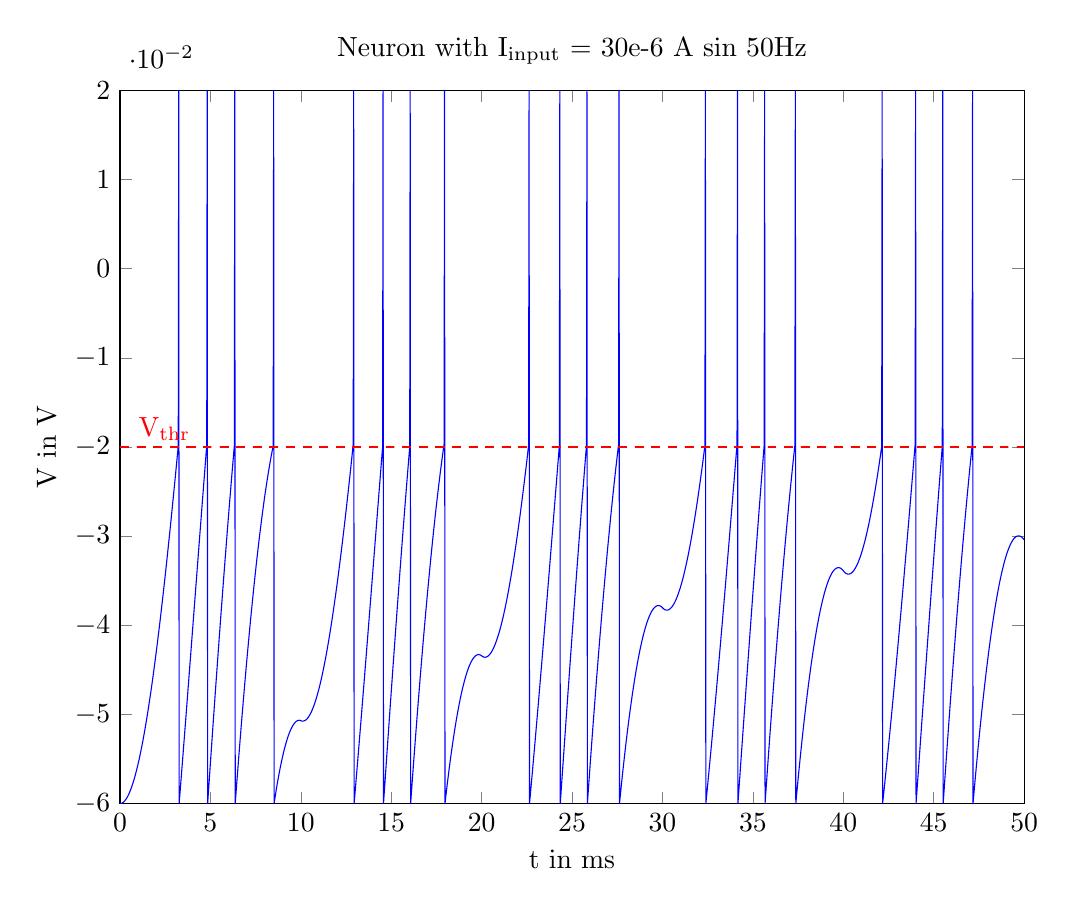
\begin{tikzpicture}

\begin{axis}[%
width=4.520833in,
height=3.565625in,
at={(0.758333in,0.48125in)},
scale only axis,
separate axis lines,
every outer x axis line/.append style={black},
every x tick label/.append style={font=\color{black}},
xmin=0,
xmax=50,
xlabel={t in ms},
every outer y axis line/.append style={black},
every y tick label/.append style={font=\color{black}},
ymin=-0.06,
ymax=0.02,
ylabel={V in V},
title={$\text{Neuron with I}_{\text{input}}\text{ = 30e-6 A sin 50Hz}$}
]
\addplot [color=blue,solid,forget plot]
  table[row sep=crcr]{%
0	-0.06\\
0.025	-0.06\\
0.05	-0.0599941095743335\\
0.075	-0.0599823438124138\\
0.1	-0.0599647181292575\\
0.125	-0.0599412482646258\\
0.15	-0.0599119502821449\\
0.175	-0.0598768405684073\\
0.2	-0.059835935832052\\
0.225	-0.0597892531028249\\
0.25	-0.0597368097306194\\
0.275	-0.059678623384497\\
0.3	-0.0596147120516873\\
0.325	-0.0595450940365692\\
0.35	-0.0594697879596315\\
0.375	-0.0593888127564141\\
0.4	-0.0593021876764297\\
0.425	-0.0592099322820654\\
0.45	-0.0591120664474653\\
0.475	-0.0590086103573935\\
0.5	-0.0588995845060773\\
0.525	-0.0587850096960319\\
0.55	-0.0586649070368652\\
0.575	-0.0585392979440635\\
0.6	-0.0584082041377584\\
0.625	-0.0582716476414748\\
0.65	-0.058129650780859\\
0.675	-0.0579822361823894\\
0.7	-0.0578294267720675\\
0.725	-0.0576712457740899\\
0.75	-0.0575077167095029\\
0.775	-0.0573388633948372\\
0.8	-0.0571647099407253\\
0.825	-0.0569852807504998\\
0.85	-0.0568006005187738\\
0.875	-0.0566106942300029\\
0.9	-0.0564155871570291\\
0.925	-0.0562153048596071\\
0.95	-0.0560098731829122\\
0.975	-0.0557993182560307\\
1	-0.0555836664904322\\
1.025	-0.055362944578425\\
1.05	-0.0551371794915927\\
1.075	-0.0549063984792151\\
1.1	-0.0546706290666701\\
1.125	-0.0544298990538195\\
1.15	-0.0541842365133768\\
1.175	-0.0539336697892589\\
1.2	-0.0536782274949201\\
1.225	-0.0534179385116693\\
1.25	-0.0531528319869711\\
1.275	-0.0528829373327299\\
1.3	-0.0526082842235569\\
1.325	-0.0523289025950219\\
1.35	-0.0520448226418878\\
1.375	-0.0517560748163293\\
1.4	-0.0514626898261354\\
1.425	-0.0511646986328962\\
1.45	-0.0508621324501737\\
1.475	-0.0505550227416563\\
1.5	-0.0502434012192988\\
1.525	-0.0499272998414459\\
1.55	-0.0496067508109407\\
1.575	-0.0492817865732179\\
1.6	-0.0489524398143819\\
1.625	-0.0486187434592697\\
1.65	-0.0482807306694988\\
1.675	-0.0479384348415008\\
1.7	-0.0475918896045395\\
1.725	-0.0472411288187153\\
1.75	-0.0468861865729548\\
1.775	-0.0465270971829854\\
1.8	-0.0461638951892973\\
1.825	-0.0457966153550898\\
1.85	-0.0454252926642048\\
1.875	-0.0450499623190457\\
1.9	-0.0446706597384833\\
1.925	-0.044287420555748\\
1.95	-0.043900280616308\\
1.975	-0.0435092759757347\\
2	-0.0431144428975555\\
2.025	-0.0427158178510923\\
2.05	-0.042313437509288\\
2.075	-0.0419073387465204\\
2.1	-0.0414975586364026\\
2.125	-0.0410841344495718\\
2.15	-0.0406671036514655\\
2.175	-0.0402465039000851\\
2.2	-0.0398223730437478\\
2.225	-0.039394749118827\\
2.25	-0.0389636703474796\\
2.275	-0.0385291751353632\\
2.3	-0.038091302069341\\
2.325	-0.0376500899151749\\
2.35	-0.0372055776152085\\
2.375	-0.0367578042860381\\
2.4	-0.0363068092161733\\
2.425	-0.0358526318636864\\
2.45	-0.0353953118538513\\
2.475	-0.0349348889767725\\
2.5	-0.0344714031850024\\
2.525	-0.03400489459115\\
2.55	-0.0335354034654782\\
2.575	-0.0330629702334921\\
2.6	-0.032587635473517\\
2.625	-0.0321094399142672\\
2.65	-0.0316284244324048\\
2.675	-0.0311446300500898\\
2.7	-0.0306580979325209\\
2.725	-0.0301688693854667\\
2.75	-0.0296769858527892\\
2.775	-0.0291824889139572\\
2.8	-0.0286854202815525\\
2.825	-0.0281858217987667\\
2.85	-0.0276837354368906\\
2.875	-0.0271792032927947\\
2.9	-0.0266722675864021\\
2.925	-0.0261629706581543\\
2.95	-0.0256513549664683\\
2.975	-0.0251374630851868\\
3	-0.0246213377010213\\
3.025	-0.0241030216109875\\
3.05	-0.0235825577198345\\
3.075	-0.0230599890374661\\
3.1	-0.0225353586763568\\
3.125	-0.02200870984896\\
3.15	-0.0214800858651107\\
3.175	-0.0209495301294217\\
3.2	-0.020417086138674\\
3.225	-0.0198827974792008\\
3.25	0.02\\
3.275	-0.06\\
3.3	-0.0593574618608512\\
3.325	-0.0587135116859461\\
3.35	-0.0580681928263411\\
3.375	-0.0574215487084466\\
3.4	-0.0567736228313709\\
3.425	-0.0561244587642596\\
3.45	-0.0554741001436306\\
3.475	-0.054822590670705\\
3.5	-0.0541699741087338\\
3.525	-0.0535162942803207\\
3.55	-0.0528615950647414\\
3.575	-0.052205920395259\\
3.6	-0.0515493142564367\\
3.625	-0.0508918206814461\\
3.65	-0.0502334837493737\\
3.675	-0.0495743475825237\\
3.7	-0.0489144563437184\\
3.725	-0.0482538542335961\\
3.75	-0.0475925854879063\\
3.775	-0.0469306943748031\\
3.8	-0.046268225192136\\
3.825	-0.0456052222647395\\
3.85	-0.0449417299417203\\
3.875	-0.0442777925937436\\
3.9	-0.0436134546103174\\
3.925	-0.0429487603970759\\
3.95	-0.0422837543730621\\
3.975	-0.0416184809680088\\
4	-0.0409529846196196\\
4.025	-0.0402873097708492\\
4.05	-0.0396215008671828\\
4.075	-0.0389556023539161\\
4.1	-0.0382896586734346\\
4.125	-0.0376237142624933\\
4.15	-0.0369578135494968\\
4.175	-0.0362920009517798\\
4.2	-0.0356263208728876\\
4.225	-0.0349608176998589\\
4.25	-0.0342955358005079\\
4.275	-0.0336305195207083\\
4.3	-0.0329658131816792\\
4.325	-0.0323014610772709\\
4.35	-0.0316375074712541\\
4.375	-0.0309739965946097\\
4.4	-0.0303109726428207\\
4.425	-0.0296484797731672\\
4.45	-0.0289865621020221\\
4.475	-0.028325263702151\\
4.5	-0.0276646286000132\\
4.525	-0.0270047007730668\\
4.55	-0.0263455241470758\\
4.575	-0.0256871425934207\\
4.6	-0.0250295999264126\\
4.625	-0.0243729399006107\\
4.65	-0.023717206208143\\
4.675	-0.0230624424760313\\
4.7	-0.0224086922635199\\
4.725	-0.0217559990594088\\
4.75	-0.0211044062793906\\
4.775	-0.0204539572633923\\
4.8	-0.0198046952729216\\
4.825	0.02\\
4.85	-0.06\\
4.875	-0.0592508325937785\\
4.9	-0.0585032837351135\\
4.925	-0.0577573956055015\\
4.95	-0.0570132102938242\\
4.975	-0.0562707697937284\\
5	-0.0555301160010105\\
5.025	-0.0547912907110079\\
5.05	-0.0540543356159968\\
5.075	-0.0533192923025956\\
5.1	-0.0525862022491756\\
5.125	-0.0518551068232784\\
5.15	-0.0511260472790396\\
5.175	-0.0503990647546205\\
5.2	-0.0496742002696461\\
5.225	-0.0489514947226508\\
5.25	-0.0482309888885319\\
5.275	-0.0475127234160108\\
5.3	-0.046796738825101\\
5.325	-0.046083075504586\\
5.35	-0.0453717737095032\\
5.375	-0.0446628735586381\\
5.4	-0.0439564150320253\\
5.425	-0.0432524379684593\\
5.45	-0.0425509820630137\\
5.475	-0.0418520868645688\\
5.5	-0.041155791773349\\
5.525	-0.0404621360384692\\
5.55	-0.0397711587554907\\
5.575	-0.0390828988639859\\
5.6	-0.0383973951451138\\
5.625	-0.0377146862192045\\
5.65	-0.037034810543354\\
5.675	-0.0363578064090293\\
5.7	-0.0356837119396832\\
5.725	-0.0350125650883799\\
5.75	-0.0343444036354315\\
5.775	-0.0336792651860447\\
5.8	-0.0330171871679782\\
5.825	-0.0323582068292118\\
5.85	-0.0317023612356261\\
5.875	-0.0310496872686936\\
5.9	-0.0304002216231817\\
5.925	-0.029754000804866\\
5.95	-0.0291110611282571\\
5.975	-0.0284714387143377\\
6	-0.0278351694883126\\
6.025	-0.0272022891773705\\
6.05	-0.0265728333084579\\
6.075	-0.0259468372060661\\
6.1	-0.0253243359900298\\
6.125	-0.0247053645733391\\
6.15	-0.0240899576599639\\
6.175	-0.0234781497426915\\
6.2	-0.0228699751009775\\
6.225	-0.0222654677988089\\
6.25	-0.0216646616825818\\
6.275	-0.0210675903789918\\
6.3	-0.0204742872929386\\
6.325	-0.0198847856054433\\
6.35	0.02\\
6.375	-0.06\\
6.4	-0.0593188926196312\\
6.425	-0.0586419750987326\\
6.45	-0.0579692788231516\\
6.475	-0.0573008349442732\\
6.5	-0.056636674377034\\
6.525	-0.0559768277979502\\
6.55	-0.0553213256431608\\
6.575	-0.0546701981064864\\
6.6	-0.0540234751375018\\
6.625	-0.0533811864396252\\
6.65	-0.0527433614682215\\
6.675	-0.0521100294287223\\
6.7	-0.0514812192747604\\
6.725	-0.0508569597063206\\
6.75	-0.050237279167906\\
6.775	-0.0496222058467206\\
6.8	-0.0490117676708677\\
6.825	-0.048405992307564\\
6.85	-0.0478049071613709\\
6.875	-0.0472085393724413\\
6.9	-0.0466169158147833\\
6.925	-0.0460300630945404\\
6.95	-0.0454480075482884\\
6.975	-0.0448707752413489\\
7	-0.0442983919661199\\
7.025	-0.0437308832404234\\
7.05	-0.0431682743058698\\
7.075	-0.0426105901262398\\
7.1	-0.0420578553858836\\
7.125	-0.0415100944881371\\
7.15	-0.0409673315537562\\
7.175	-0.0404295904193681\\
7.2	-0.0398968946359405\\
7.225	-0.0393692674672688\\
7.25	-0.0388467318884808\\
7.275	-0.0383293105845596\\
7.3	-0.0378170259488843\\
7.325	-0.0373099000817892\\
7.35	-0.036807954789141\\
7.375	-0.0363112115809342\\
7.4	-0.0358196916699051\\
7.425	-0.0353334159701643\\
7.45	-0.0348524050958476\\
7.475	-0.0343766793597856\\
7.5	-0.0339062587721922\\
7.525	-0.0334411630393718\\
7.55	-0.0329814115624452\\
7.575	-0.0325270234360949\\
7.6	-0.0320780174473288\\
7.625	-0.031634412074264\\
7.65	-0.0311962254849286\\
7.675	-0.030763475536084\\
7.7	-0.0303361797720653\\
7.725	-0.0299143554236424\\
7.75	-0.0294980194068994\\
7.775	-0.0290871883221346\\
7.8	-0.0286818784527789\\
7.825	-0.0282821057643354\\
7.85	-0.0278878859033376\\
7.875	-0.0274992341963274\\
7.9	-0.0271161656488542\\
7.925	-0.0267386949444924\\
7.95	-0.0263668364438796\\
7.975	-0.0260006041837755\\
8	-0.0256400118761396\\
8.025	-0.0252850729072298\\
8.05	-0.0249358003367219\\
8.075	-0.0245922068968476\\
8.1	-0.0242543049915548\\
8.125	-0.0239221066956868\\
8.15	-0.0235956237541829\\
8.175	-0.0232748675812989\\
8.2	-0.0229598492598483\\
8.225	-0.0226505795404644\\
8.25	-0.0223470688408826\\
8.275	-0.0220493272452434\\
8.3	-0.0217573645034165\\
8.325	-0.0214711900303452\\
8.35	-0.0211908129054118\\
8.375	-0.020916241871824\\
8.4	-0.0206474853360217\\
8.425	-0.0203845513671054\\
8.45	-0.0201274476962847\\
8.475	-0.0198761817163485\\
8.5	0.02\\
8.525	-0.06\\
8.55	-0.0596647660344967\\
8.575	-0.0593356497420185\\
8.6	-0.0590126561815231\\
8.625	-0.0586957900723955\\
8.65	-0.0583850557940614\\
8.675	-0.0580804573856225\\
8.7	-0.0577819985455118\\
8.725	-0.057489682631172\\
8.75	-0.0572035126587529\\
8.775	-0.0569234913028322\\
8.8	-0.0566496208961562\\
8.825	-0.0563819034294023\\
8.85	-0.056120340550963\\
8.875	-0.0558649335667512\\
8.9	-0.0556156834400262\\
8.925	-0.0553725907912421\\
8.95	-0.0551356558979171\\
8.975	-0.0549048786945237\\
9	-0.0546802587724012\\
9.025	-0.054461795379689\\
9.05	-0.0542494874212814\\
9.075	-0.054043333458804\\
9.1	-0.0538433317106111\\
9.125	-0.0536494800518052\\
9.15	-0.0534617760142768\\
9.175	-0.0532802167867671\\
9.2	-0.0531047992149505\\
9.225	-0.0529355198015394\\
9.25	-0.0527723747064108\\
9.275	-0.0526153597467529\\
9.3	-0.0524644703972341\\
9.325	-0.0523197017901937\\
9.35	-0.0521810487158522\\
9.375	-0.0520485056225452\\
9.4	-0.0519220666169767\\
9.425	-0.051801725464495\\
9.45	-0.0516874755893888\\
9.475	-0.0515793100752058\\
9.5	-0.0514772216650912\\
9.525	-0.0513812027621482\\
9.55	-0.0512912454298202\\
9.575	-0.0512073413922924\\
9.6	-0.0511294820349168\\
9.625	-0.0510576584046563\\
9.65	-0.0509918612105513\\
9.675	-0.0509320808242066\\
9.7	-0.0508783072802998\\
9.725	-0.0508305302771102\\
9.75	-0.0507887391770689\\
9.775	-0.0507529230073304\\
9.8	-0.0507230704603637\\
9.825	-0.0506991698945658\\
9.85	-0.050681209334895\\
9.875	-0.0506691764735256\\
9.9	-0.0506630586705225\\
9.925	-0.0506628429545376\\
9.95	-0.050668516023526\\
9.975	-0.0506800642454833\\
10	-0.0506974736592031\\
10.025	-0.0507207299750551\\
10.05	-0.0507380377244509\\
10.075	-0.0507494121421559\\
10.1	-0.0507548687881753\\
10.125	-0.0507544235468963\\
10.15	-0.0507480926262097\\
10.175	-0.050735892556612\\
10.2	-0.0507178401902861\\
10.225	-0.0506939527001634\\
10.25	-0.0506642475789646\\
10.275	-0.0506287426382213\\
10.3	-0.0505874560072774\\
10.325	-0.0505404061322703\\
10.35	-0.0504876117750933\\
10.375	-0.0504290920123373\\
10.4	-0.0503648662342131\\
10.425	-0.0502949541434543\\
10.45	-0.0502193757542008\\
10.475	-0.0501381513908621\\
10.5	-0.0500513016869622\\
10.525	-0.0499588475839646\\
10.55	-0.0498608103300781\\
10.575	-0.0497572114790433\\
10.6	-0.0496480728889008\\
10.625	-0.0495334167207393\\
10.65	-0.0494132654374253\\
10.675	-0.0492876418023144\\
10.7	-0.0491565688779426\\
10.725	-0.0490200700247004\\
10.75	-0.0488781688994868\\
10.775	-0.0487308894543461\\
10.8	-0.0485782559350855\\
10.825	-0.0484202928798741\\
10.85	-0.0482570251178247\\
10.875	-0.0480884777675561\\
10.9	-0.0479146762357384\\
10.925	-0.0477356462156196\\
10.95	-0.0475514136855347\\
10.975	-0.0473620049073967\\
11	-0.0471674464251698\\
11.025	-0.0469677650633257\\
11.05	-0.0467629879252812\\
11.075	-0.0465531423918194\\
11.1	-0.0463382561194929\\
11.125	-0.0461183570390102\\
11.15	-0.0458934733536045\\
11.175	-0.0456636335373861\\
11.2	-0.0454288663336769\\
11.225	-0.0451892007533292\\
11.25	-0.0449446660730269\\
11.275	-0.0446952918335705\\
11.3	-0.0444411078381454\\
11.325	-0.044182144150574\\
11.35	-0.043918431093551\\
11.375	-0.0436499992468633\\
11.4	-0.0433768794455931\\
11.425	-0.0430991027783053\\
11.45	-0.0428167005852192\\
11.475	-0.0425297044563642\\
11.5	-0.04223814622972\\
11.525	-0.041942057989341\\
11.55	-0.0416414720634661\\
11.575	-0.041336421022612\\
11.6	-0.0410269376776525\\
11.625	-0.0407130550778821\\
11.65	-0.0403948065090646\\
11.675	-0.0400722254914677\\
11.7	-0.0397453457778815\\
11.725	-0.039414201351624\\
11.75	-0.0390788264245311\\
11.775	-0.0387392554349329\\
11.8	-0.0383955230456149\\
11.825	-0.0380476641417666\\
11.85	-0.0376957138289148\\
11.875	-0.037339707430844\\
11.9	-0.0369796804875021\\
11.925	-0.0366156687528943\\
11.95	-0.0362477081929614\\
11.975	-0.0358758349834465\\
12	-0.035500085507748\\
12.025	-0.0351204963547593\\
12.05	-0.0347371043166958\\
12.075	-0.0343499463869097\\
12.1	-0.0339590597576909\\
12.125	-0.033564481818057\\
12.15	-0.0331662501515294\\
12.175	-0.0327644025338988\\
12.2	-0.0323589769309771\\
12.225	-0.0319500114963381\\
12.25	-0.0315375445690469\\
12.275	-0.0311216146713767\\
12.3	-0.0307022605065144\\
12.325	-0.0302795209562553\\
12.35	-0.0298534350786863\\
12.375	-0.0294240421058572\\
12.4	-0.0289913814414429\\
12.425	-0.0285554926583927\\
12.45	-0.0281164154965709\\
12.475	-0.0276741898603853\\
12.5	-0.0272288558164062\\
12.525	-0.0267804535909752\\
12.55	-0.0263290235678039\\
12.575	-0.025874606285562\\
12.6	-0.0254172424354567\\
12.625	-0.024956972858802\\
12.65	-0.0244938385445783\\
12.675	-0.0240278806269829\\
12.7	-0.0235591403829717\\
12.725	-0.0230876592297914\\
12.75	-0.0226134787225031\\
12.775	-0.0221366405514968\\
12.8	-0.0216571865399982\\
12.825	-0.0211751586415664\\
12.85	-0.0206905989375833\\
12.875	-0.0202035496347356\\
12.9	-0.0197140530624882\\
12.925	0.02\\
12.95	-0.06\\
12.975	-0.0594002365061347\\
13	-0.0587984541884168\\
13.025	-0.0581946953071645\\
13.05	-0.057589002231771\\
13.075	-0.0569814174381228\\
13.1	-0.0563719835060119\\
13.125	-0.0557607431165409\\
13.15	-0.0551477390495227\\
13.175	-0.0545330141808726\\
13.2	-0.0539166114799963\\
13.225	-0.0532985740071698\\
13.25	-0.0526789449109157\\
13.275	-0.0520577674253729\\
13.3	-0.0514350848676606\\
13.325	-0.0508109406352385\\
13.35	-0.0501853782032603\\
13.375	-0.0495584411219235\\
13.4	-0.0489301730138141\\
13.425	-0.0483006175712467\\
13.45	-0.0476698185536002\\
13.475	-0.0470378197846497\\
13.5	-0.0464046651498936\\
13.525	-0.0457703985938776\\
13.55	-0.0451350641175144\\
13.575	-0.0444987057754001\\
13.6	-0.0438613676731274\\
13.625	-0.0432230939645951\\
13.65	-0.0425839288493148\\
13.675	-0.0419439165697149\\
13.7	-0.0413031014084417\\
13.725	-0.0406615276856576\\
13.75	-0.0400192397563377\\
13.775	-0.0393762820075634\\
13.8	-0.0387326988558144\\
13.825	-0.0380885347442587\\
13.85	-0.0374438341400407\\
13.875	-0.0367986415315682\\
13.9	-0.0361530014257974\\
13.925	-0.0355069583455173\\
13.95	-0.0348605568266323\\
13.975	-0.0342138414154451\\
14	-0.0335668566659373\\
14.025	-0.0329196471370511\\
14.05	-0.0322722573899692\\
14.075	-0.0316247319853956\\
14.1	-0.0309771154808353\\
14.125	-0.0303294524278755\\
14.15	-0.0296817873694656\\
14.175	-0.0290341648371986\\
14.2	-0.0283866293485929\\
14.225	-0.027739225404375\\
14.25	-0.0270919974857626\\
14.275	-0.02644499005175\\
14.3	-0.0257982475363932\\
14.325	-0.0251518143460982\\
14.35	-0.0245057348569093\\
14.375	-0.0238600534118007\\
14.4	-0.0232148143179688\\
14.425	-0.0225700618441274\\
14.45	-0.0219258402178049\\
14.475	-0.0212821936226443\\
14.5	-0.0206391661957053\\
14.525	-0.0199968020247697\\
14.55	0.02\\
14.575	-0.06\\
14.6	-0.0592566751894755\\
14.625	-0.058514447475516\\
14.65	-0.057773360014111\\
14.675	-0.0570334558974843\\
14.7	-0.0562947781514193\\
14.725	-0.0555573697325885\\
14.75	-0.0548212735258873\\
14.775	-0.0540865323417727\\
14.8	-0.0533531889136061\\
14.825	-0.0526212858950009\\
14.85	-0.0518908658571755\\
14.875	-0.051161971286311\\
14.9	-0.0504346445809147\\
14.925	-0.0497089280491881\\
14.95	-0.0489848639064017\\
14.975	-0.0482624942722744\\
15	-0.0475418611683601\\
15.025	-0.0468230065154392\\
15.05	-0.046105972130917\\
15.075	-0.0453907997262285\\
15.1	-0.0446775309042494\\
15.125	-0.0439662071567145\\
15.15	-0.0432568698616422\\
15.175	-0.0425495602807666\\
15.2	-0.0418443195569768\\
15.225	-0.0411411887117631\\
15.25	-0.0404402086426715\\
15.275	-0.039741420120765\\
15.3	-0.0390448637880934\\
15.325	-0.0383505801551708\\
15.35	-0.0376586095984616\\
15.375	-0.0369689923578741\\
15.4	-0.0362817685342632\\
15.425	-0.0355969780869417\\
15.45	-0.0349146608311998\\
15.475	-0.0342348564358344\\
15.5	-0.0335576044206865\\
15.525	-0.0328829441541884\\
15.55	-0.0322109148509205\\
15.575	-0.0315415555691772\\
15.6	-0.0308749052085421\\
15.625	-0.0302110025074742\\
15.65	-0.0295498860409031\\
15.675	-0.0288915942178345\\
15.7	-0.0282361652789663\\
15.725	-0.0275836372943148\\
15.75	-0.0269340481608517\\
15.775	-0.0262874356001513\\
15.8	-0.0256438371560495\\
15.825	-0.0250032901923129\\
15.85	-0.0243658318903194\\
15.875	-0.0237314992467503\\
15.9	-0.0231003290712932\\
15.925	-0.0224723579843572\\
15.95	-0.0218476224147996\\
15.975	-0.0212261585976639\\
16	-0.0206080025719305\\
16.025	-0.0199931901782793\\
16.05	0.02\\
16.075	-0.06\\
16.1	-0.0592923658769789\\
16.125	-0.0585884743855707\\
16.15	-0.0578883596976649\\
16.175	-0.0571920557752984\\
16.2	-0.0564995963685028\\
16.225	-0.0558110150131654\\
16.25	-0.0551263450289024\\
16.275	-0.0544456195169466\\
16.3	-0.0537688713580485\\
16.325	-0.0530961332103904\\
16.35	-0.0524274375075155\\
16.375	-0.0517628164562701\\
16.4	-0.0511023020347606\\
16.425	-0.0504459259903242\\
16.45	-0.0497937198375142\\
16.475	-0.0491457148560999\\
16.5	-0.0485019420890812\\
16.525	-0.0478624323407172\\
16.55	-0.0472272161745709\\
16.575	-0.046596323911568\\
16.6	-0.0459697856280707\\
16.625	-0.0453476311539677\\
16.65	-0.0447298900707781\\
16.675	-0.0441165917097725\\
16.7	-0.043507765150108\\
16.725	-0.0429034392169798\\
16.75	-0.0423036424797885\\
16.775	-0.0417084032503235\\
16.8	-0.0411177495809615\\
16.825	-0.0405317092628826\\
16.85	-0.0399503098243012\\
16.875	-0.0393735785287143\\
16.9	-0.0388015423731656\\
16.925	-0.0382342280865267\\
16.95	-0.0376716621277948\\
16.975	-0.0371138706844065\\
17	-0.0365608796705699\\
17.025	-0.0360127147256123\\
17.05	-0.0354694012123457\\
17.075	-0.0349309642154495\\
17.1	-0.0343974285398702\\
17.125	-0.0338688187092388\\
17.15	-0.0333451589643051\\
17.175	-0.0328264732613906\\
17.2	-0.032312785270858\\
17.225	-0.031804118375599\\
17.25	-0.0313004956695402\\
17.275	-0.0308019399561663\\
17.3	-0.030308473747062\\
17.325	-0.0298201192604715\\
17.35	-0.0293368984198766\\
17.375	-0.028858832852593\\
17.4	-0.0283859438883847\\
17.425	-0.0279182525580977\\
17.45	-0.0274557795923111\\
17.475	-0.0269985454200079\\
17.5	-0.026546570167264\\
17.525	-0.0260998736559559\\
17.55	-0.0256584754024879\\
17.575	-0.0252223946165375\\
17.6	-0.0247916501998203\\
17.625	-0.0243662607448742\\
17.65	-0.0239462445338623\\
17.675	-0.0235316195373953\\
17.7	-0.0231224034133734\\
17.725	-0.0227186135058472\\
17.75	-0.0223202668438988\\
17.775	-0.0219273801405414\\
17.8	-0.0215399697916397\\
17.825	-0.0211580518748491\\
17.85	-0.0207816421485749\\
17.875	-0.0204107560509517\\
17.9	-0.020045408698842\\
17.925	-0.0196856148868551\\
17.95	0.02\\
17.975	-0.06\\
18	-0.0595544092028235\\
18.025	-0.0591146842405971\\
18.05	-0.0586808376417557\\
18.075	-0.0582528816086188\\
18.1	-0.0578308280165466\\
18.125	-0.0574146884131161\\
18.15	-0.0570044740173186\\
18.175	-0.0566001957187768\\
18.2	-0.0562018640769825\\
18.225	-0.0558094893205558\\
18.25	-0.0554230813465237\\
18.275	-0.0550426497196205\\
18.3	-0.0546682036716076\\
18.325	-0.0542997521006158\\
18.35	-0.0539373035705068\\
18.375	-0.0535808663102562\\
18.4	-0.0532304482133578\\
18.425	-0.0528860568372481\\
18.45	-0.0525476994027521\\
18.475	-0.0522153827935498\\
18.5	-0.0518891135556643\\
18.525	-0.0515688978969705\\
18.55	-0.0512547416867247\\
18.575	-0.050946650455116\\
18.6	-0.0506446293928379\\
18.625	-0.050348683350682\\
18.65	-0.0500588168391522\\
18.675	-0.0497750340281005\\
18.7	-0.0494973387463837\\
18.725	-0.0492257344815416\\
18.75	-0.0489602243794966\\
18.775	-0.0487008112442741\\
18.8	-0.0484474975377444\\
18.825	-0.0482002853793865\\
18.85	-0.0479591765460723\\
18.875	-0.0477241724718727\\
18.9	-0.0474952742478849\\
18.925	-0.0472724826220812\\
18.95	-0.0470557979991791\\
18.975	-0.0468452204405325\\
19	-0.046640749664045\\
19.025	-0.0464423850441037\\
19.05	-0.0462501256115351\\
19.075	-0.046063970053582\\
19.1	-0.0458839167139022\\
19.125	-0.045709963592588\\
19.15	-0.0455421083462077\\
19.175	-0.0453803482878682\\
19.2	-0.0452246803872988\\
19.225	-0.0450751012709569\\
19.25	-0.0449316072221547\\
19.275	-0.0447941941812074\\
19.3	-0.0446628577456026\\
19.325	-0.0445375931701912\\
19.35	-0.0444183953673997\\
19.375	-0.0443052589074638\\
19.4	-0.0441981780186831\\
19.425	-0.0440971465876971\\
19.45	-0.0440021581597829\\
19.475	-0.0439132059391739\\
19.5	-0.0438302827893993\\
19.525	-0.0437533812336457\\
19.55	-0.0436824934551389\\
19.575	-0.0436176112975478\\
19.6	-0.043558726265409\\
19.625	-0.0435058295245723\\
19.65	-0.0434589119026675\\
19.675	-0.0434179638895925\\
19.7	-0.0433829756380223\\
19.725	-0.0433539369639383\\
19.75	-0.04333083734718\\
19.775	-0.0433136659320162\\
19.8	-0.0433024115277378\\
19.825	-0.0432970626092715\\
19.85	-0.0432976073178139\\
19.875	-0.0433040334614872\\
19.9	-0.0433163285160141\\
19.925	-0.0433344796254155\\
19.95	-0.0433584736027268\\
19.975	-0.0433882969307361\\
20	-0.0434239357627427\\
20.025	-0.0434653759233359\\
20.05	-0.043500822057861\\
20.075	-0.0435302895147325\\
20.1	-0.0435537939673204\\
20.125	-0.0435713514130935\\
20.15	-0.0435829781727415\\
20.175	-0.0435886908892774\\
20.2	-0.0435885065271199\\
20.225	-0.0435824423711551\\
20.25	-0.0435705160257788\\
20.275	-0.0435527454139185\\
20.3	-0.0435291487760353\\
20.325	-0.0434997446691063\\
20.35	-0.0434645519655872\\
20.375	-0.043423589852355\\
20.4	-0.0433768778296307\\
20.425	-0.0433244357098834\\
20.45	-0.0432662836167138\\
20.475	-0.0432024419837188\\
20.5	-0.0431329315533368\\
20.525	-0.0430577733756733\\
20.55	-0.0429769888073075\\
20.575	-0.0428905995100797\\
20.6	-0.0427986274498596\\
20.625	-0.0427010948952956\\
20.65	-0.0425980244165453\\
20.675	-0.0424894388839865\\
20.7	-0.0423753614669106\\
20.725	-0.0422558156321959\\
20.75	-0.0421308251429636\\
20.775	-0.0420004140572142\\
20.8	-0.0418646067264464\\
20.825	-0.0417234277942567\\
20.85	-0.0415769021949213\\
20.875	-0.04142505515196\\
20.9	-0.0412679121766813\\
20.925	-0.0411054990667101\\
20.95	-0.0409378419044975\\
20.975	-0.040764967055812\\
21	-0.0405869011682141\\
21.025	-0.0404036711695124\\
21.05	-0.0402153042662024\\
21.075	-0.0400218279418883\\
21.1	-0.0398232699556866\\
21.125	-0.0396196583406135\\
21.15	-0.0394110214019538\\
21.175	-0.0391973877156145\\
21.2	-0.0389787861264597\\
21.225	-0.0387552457466301\\
21.25	-0.0385267959538445\\
21.275	-0.0382934663896861\\
21.3	-0.0380552869578707\\
21.325	-0.0378122878225\\
21.35	-0.0375644994062972\\
21.375	-0.0373119523888276\\
21.4	-0.0370546777047024\\
21.425	-0.0367927065417669\\
21.45	-0.0365260703392722\\
21.475	-0.036254800786032\\
21.5	-0.0359789298185636\\
21.525	-0.0356984896192125\\
21.55	-0.0354135126142629\\
21.575	-0.0351240314720318\\
21.6	-0.0348300791009488\\
21.625	-0.0345316886476201\\
21.65	-0.0342288934948784\\
21.675	-0.0339217272598169\\
21.7	-0.0336102237918098\\
21.725	-0.0332944171705175\\
21.75	-0.0329743417038774\\
21.775	-0.0326500319260808\\
21.8	-0.0323215225955349\\
21.825	-0.0319888486928118\\
21.85	-0.0316520454185825\\
21.875	-0.0313111481915374\\
21.9	-0.0309661926462939\\
21.925	-0.030617214631289\\
21.95	-0.0302642502066601\\
21.975	-0.029907335642111\\
22	-0.0295465074147659\\
22.025	-0.0291818022070096\\
22.05	-0.0288132569043155\\
22.075	-0.0284409085930603\\
22.1	-0.0280647945583262\\
22.125	-0.0276849522816906\\
22.15	-0.027301419439004\\
22.175	-0.0269142338981547\\
22.2	-0.0265234337168223\\
22.225	-0.0261290571402187\\
22.25	-0.0257311425988179\\
22.275	-0.0253297287060732\\
22.3	-0.0249248542561241\\
22.325	-0.0245165582214911\\
22.35	-0.0241048797507589\\
22.375	-0.0236898581662497\\
22.4	-0.0232715329616844\\
22.425	-0.0228499437998336\\
22.45	-0.0224251305101582\\
22.475	-0.0219971330864386\\
22.5	-0.0215659916843944\\
22.525	-0.0211317466192935\\
22.55	-0.0206944383635513\\
22.575	-0.0202541075443201\\
22.6	-0.0198107949410679\\
22.625	0.02\\
22.65	-0.06\\
22.675	-0.059445276678766\\
22.7	-0.0588879929446254\\
22.725	-0.058328189660041\\
22.75	-0.057765907826677\\
22.775	-0.0572011885829103\\
22.8	-0.0566340732013332\\
22.825	-0.056064603086248\\
22.85	-0.0554928197711532\\
22.875	-0.0549187649162216\\
22.9	-0.0543424803057705\\
22.925	-0.0537640078457243\\
22.95	-0.0531833895610694\\
22.975	-0.0526006675933014\\
23	-0.0520158841978656\\
23.025	-0.0514290817415897\\
23.05	-0.0508403027001101\\
23.075	-0.0502495896552911\\
23.1	-0.0496569852926372\\
23.125	-0.0490625323986997\\
23.15	-0.048466273858476\\
23.175	-0.0478682526528036\\
23.2	-0.0472685118557474\\
23.225	-0.0466670946319815\\
23.25	-0.0460640442341654\\
23.275	-0.0454594040003145\\
23.3	-0.0448532173511649\\
23.325	-0.044245527787534\\
23.35	-0.0436363788876751\\
23.375	-0.0430258143046272\\
23.4	-0.0424138777635611\\
23.425	-0.0418006130591193\\
23.45	-0.0411860640527531\\
23.475	-0.0405702746700547\\
23.5	-0.0399532888980851\\
23.525	-0.0393351507826986\\
23.55	-0.0387159044258634\\
23.575	-0.0380955939829782\\
23.6	-0.0374742636601866\\
23.625	-0.0368519577116866\\
23.65	-0.0362287204370386\\
23.675	-0.0356045961784694\\
23.7	-0.0349796293181743\\
23.725	-0.0343538642756159\\
23.75	-0.033727345504821\\
23.775	-0.0331001174916755\\
23.8	-0.0324722247512162\\
23.825	-0.031843711824922\\
23.85	-0.0312146232780024\\
23.875	-0.030585003696685\\
23.9	-0.0299548976855014\\
23.925	-0.029324349864572\\
23.95	-0.0286934048668894\\
23.975	-0.0280621073356015\\
24	-0.0274305019212934\\
24.025	-0.0267986332792688\\
24.05	-0.0261665460668314\\
24.075	-0.0255342849405655\\
24.1	-0.0249018945536174\\
24.125	-0.0242694195529756\\
24.15	-0.023636904576753\\
24.175	-0.0230043942514677\\
24.2	-0.0223719331893264\\
24.225	-0.0217395659855066\\
24.25	-0.0211073372154414\\
24.275	-0.0204752914321046\\
24.3	-0.0198434731632969\\
24.325	0.02\\
24.35	-0.06\\
24.375	-0.0592655828920337\\
24.4	-0.0585318299745012\\
24.425	-0.0577987849615184\\
24.45	-0.0570664915274025\\
24.475	-0.0563349933039679\\
24.5	-0.0556043338778256\\
24.525	-0.0548745567876847\\
24.55	-0.0541457055216571\\
24.575	-0.0534178235145655\\
24.6	-0.0526909541452546\\
24.625	-0.0519651407339056\\
24.65	-0.0512404265393547\\
24.675	-0.0505168547564149\\
24.7	-0.0497944685132026\\
24.725	-0.0490733108684672\\
24.75	-0.0483534248089264\\
24.775	-0.0476348532466042\\
24.8	-0.0469176390161755\\
24.825	-0.0462018248723138\\
24.85	-0.0454874534870452\\
24.875	-0.0447745674471061\\
24.9	-0.0440632092513078\\
24.925	-0.0433534213079052\\
24.95	-0.0426452459319719\\
24.975	-0.0419387253427808\\
25	-0.0412339016611902\\
25.025	-0.0405308169070372\\
25.05	-0.039829512996536\\
25.075	-0.0391300317396835\\
25.1	-0.0384324148376708\\
25.125	-0.0377367038803023\\
25.15	-0.037042940343421\\
25.175	-0.0363511655863409\\
25.2	-0.0356614208492872\\
25.225	-0.0349737472508428\\
25.25	-0.0342881857854035\\
25.275	-0.0336047773206401\\
25.3	-0.0329235625949688\\
25.325	-0.0322445822150291\\
25.35	-0.0315678766531702\\
25.375	-0.0308934862449459\\
25.4	-0.0302214511866173\\
25.425	-0.0295518115326649\\
25.45	-0.0288846071933088\\
25.475	-0.0282198779320381\\
25.5	-0.0275576633631496\\
25.525	-0.0268980029492954\\
25.55	-0.0262409359990398\\
25.575	-0.0255865016644261\\
25.6	-0.0249347389385529\\
25.625	-0.02428568665316\\
25.65	-0.0236393834762247\\
25.675	-0.0229958679095678\\
25.7	-0.0223551782864703\\
25.725	-0.0217173527693\\
25.75	-0.0210824293471494\\
25.775	-0.0204504458334833\\
25.8	-0.0198214398637982\\
25.825	0.02\\
25.85	-0.06\\
25.875	-0.0592765819361566\\
25.9	-0.058556549053976\\
25.925	-0.0578399374170834\\
25.95	-0.0571267828989439\\
25.975	-0.0564171211805978\\
26	-0.0557109877484071\\
26.025	-0.0550084178918147\\
26.05	-0.054309446701116\\
26.075	-0.0536141090652426\\
26.1	-0.0529224396695583\\
26.125	-0.0522344729936688\\
26.15	-0.0515502433092427\\
26.175	-0.0508697846778472\\
26.2	-0.0501931309487953\\
26.225	-0.0495203157570071\\
26.25	-0.0488513725208845\\
26.275	-0.0481863344401988\\
26.3	-0.0475252344939926\\
26.325	-0.0468681054384946\\
26.35	-0.0462149798050494\\
26.375	-0.0455658898980602\\
26.4	-0.0449208677929462\\
26.425	-0.0442799453341144\\
26.45	-0.0436431541329449\\
26.475	-0.0430105255657921\\
26.5	-0.0423820907719991\\
26.525	-0.0417578806519278\\
26.55	-0.0411379258650035\\
26.575	-0.0405222568277745\\
26.6	-0.0399109037119867\\
26.625	-0.0393038964426738\\
26.65	-0.0387012646962626\\
26.675	-0.0381030378986933\\
26.7	-0.0375092452235564\\
26.725	-0.0369199155902446\\
26.75	-0.0363350776621202\\
26.775	-0.0357547598446993\\
26.8	-0.0351789902838514\\
26.825	-0.0346077968640153\\
26.85	-0.034041207206431\\
26.875	-0.0334792486673887\\
26.9	-0.0329219483364934\\
26.925	-0.0323693330349462\\
26.95	-0.0318214293138432\\
26.975	-0.0312782634524898\\
27	-0.030739861456733\\
27.025	-0.03020624905731\\
27.05	-0.0296774517082141\\
27.075	-0.0291534945850783\\
27.1	-0.0286344025835749\\
27.125	-0.0281202003178342\\
27.15	-0.0276109121188791\\
27.175	-0.0271065620330781\\
27.2	-0.0266071738206163\\
27.225	-0.0261127709539829\\
27.25	-0.0256233766164781\\
27.275	-0.0251390137007369\\
27.3	-0.0246597048072712\\
27.325	-0.0241854722430302\\
27.35	-0.0237163380199789\\
27.375	-0.023252323853695\\
27.4	-0.022793451161984\\
27.425	-0.0223397410635129\\
27.45	-0.0218912143764628\\
27.475	-0.0214478916171993\\
27.5	-0.0210097929989624\\
27.525	-0.0205769384305751\\
27.55	-0.0201493475151705\\
27.575	-0.0197270395489383\\
27.6	0.02\\
27.625	-0.06\\
27.65	-0.0594908994408503\\
27.675	-0.0589874128071158\\
27.7	-0.0584895571999196\\
27.725	-0.0579973494079271\\
27.75	-0.0575108059062234\\
27.775	-0.0570299428552102\\
27.8	-0.0565547760995218\\
27.825	-0.0560853211669615\\
27.85	-0.0556215932674571\\
27.875	-0.0551636072920367\\
27.9	-0.0547113778118242\\
27.925	-0.0542649190770549\\
27.95	-0.0538242450161108\\
27.975	-0.0533893692345761\\
28	-0.0529603050143131\\
28.025	-0.052537065312558\\
28.05	-0.0521196627610367\\
28.075	-0.0517081096651016\\
28.1	-0.0513024180028882\\
28.125	-0.0509025994244919\\
28.15	-0.050508665251166\\
28.175	-0.0501206264745394\\
28.2	-0.0497384937558557\\
28.225	-0.0493622774252319\\
28.25	-0.0489919874809381\\
28.275	-0.0486276335886988\\
28.3	-0.0482692250810133\\
28.325	-0.047916770956498\\
28.35	-0.0475702798792492\\
28.375	-0.0472297601782268\\
28.4	-0.0468952198466585\\
28.425	-0.0465666665414656\\
28.45	-0.046244107582709\\
28.475	-0.0459275499530568\\
28.5	-0.0456170002972725\\
28.525	-0.0453124649217247\\
28.55	-0.045013949793917\\
28.575	-0.0447214605420403\\
28.6	-0.0444350024545449\\
28.625	-0.0441545804797347\\
28.65	-0.0438801992253823\\
28.675	-0.043611862958365\\
28.7	-0.0433495756043226\\
28.725	-0.0430933407473357\\
28.75	-0.0428431616296262\\
28.775	-0.0425990411512783\\
28.8	-0.0423609818699811\\
28.825	-0.0421289860007927\\
28.85	-0.041903055415925\\
28.875	-0.0416831916445507\\
28.9	-0.0414693958726312\\
28.925	-0.0412616689427657\\
28.95	-0.0410600113540618\\
28.975	-0.0408644232620281\\
29	-0.0406749044784868\\
29.025	-0.0404914544715094\\
29.05	-0.0403140723653722\\
29.075	-0.0401427569405346\\
29.1	-0.0399775066336374\\
29.125	-0.0398183195375239\\
29.15	-0.0396651934012813\\
29.175	-0.039518125630304\\
29.2	-0.0393771132863785\\
29.225	-0.0392421530877889\\
29.25	-0.0391132414094447\\
29.275	-0.0389903742830291\\
29.3	-0.0388735473971697\\
29.325	-0.0387627560976294\\
29.35	-0.0386579953875193\\
29.375	-0.0385592599275332\\
29.4	-0.0384665440362022\\
29.425	-0.0383798416901724\\
29.45	-0.0382991465245021\\
29.475	-0.0382244518329813\\
29.5	-0.0381557505684722\\
29.525	-0.0380930353432708\\
29.55	-0.03803629842949\\
29.575	-0.0379855317594631\\
29.6	-0.0379407269261695\\
29.625	-0.0379018751836808\\
29.65	-0.0378689674476283\\
29.675	-0.0378419942956909\\
29.7	-0.0378209459681054\\
29.725	-0.0378058123681962\\
29.75	-0.0377965830629273\\
29.775	-0.0377932472834741\\
29.8	-0.037795793925817\\
29.825	-0.0378042115513555\\
29.85	-0.0378184883875428\\
29.875	-0.0378386123285417\\
29.9	-0.0378645709359011\\
29.925	-0.0378963514392527\\
29.95	-0.0379339407370294\\
29.975	-0.0379773253972029\\
30	-0.0380264916580434\\
30.025	-0.0380814254288983\\
30.05	-0.0381303314396595\\
30.075	-0.0381732251230765\\
30.1	-0.0382101222366436\\
30.125	-0.0382410388617434\\
30.15	-0.0382659914027697\\
30.175	-0.0382849965862306\\
30.2	-0.0382980714598307\\
30.225	-0.0383052333915341\\
30.25	-0.0383065000686069\\
30.275	-0.0383018894966395\\
30.3	-0.0382914199985494\\
30.325	-0.0382751102135642\\
30.35	-0.038252979096184\\
30.375	-0.0382250459151252\\
30.4	-0.038191330252244\\
30.425	-0.0381518520014402\\
30.45	-0.0381066313675417\\
30.475	-0.0380556888651697\\
30.5	-0.037999045317584\\
30.525	-0.0379367218555099\\
30.55	-0.0378687399159445\\
30.575	-0.0377951212409451\\
30.6	-0.0377158878763978\\
30.625	-0.0376310621707675\\
30.65	-0.0375406667738285\\
30.675	-0.0374447246353766\\
30.7	-0.0373432590039221\\
30.725	-0.0372362934253649\\
30.75	-0.0371238517416497\\
30.775	-0.0370059580894036\\
30.8	-0.0368826368985553\\
30.825	-0.0367539128909353\\
30.85	-0.0366198110788582\\
30.875	-0.0364803567636871\\
30.9	-0.036335575534379\\
30.925	-0.0361854932660137\\
30.95	-0.0360301361183028\\
30.975	-0.0358695305340828\\
31	-0.0357037032377892\\
31.025	-0.0355326812339135\\
31.05	-0.0353564918054426\\
31.075	-0.0351751625122803\\
31.1	-0.0349887211896527\\
31.125	-0.0347971959464946\\
31.15	-0.0346006151638202\\
31.175	-0.0343990074930762\\
31.2	-0.0341924018544778\\
31.225	-0.0339808274353281\\
31.25	-0.0337643136883208\\
31.275	-0.0335428903298262\\
31.3	-0.0333165873381605\\
31.325	-0.033085434951839\\
31.35	-0.0328494636678129\\
31.375	-0.0326087042396895\\
31.4	-0.0323631876759372\\
31.425	-0.0321129452380736\\
31.45	-0.0318580084388381\\
31.475	-0.031598409040349\\
31.5	-0.0313341790522448\\
31.525	-0.0310653507298095\\
31.55	-0.0307919565720834\\
31.575	-0.0305140293199578\\
31.6	-0.0302316019542549\\
31.625	-0.029944707693793\\
31.65	-0.0296533799934358\\
31.675	-0.0293576525421279\\
31.7	-0.0290575592609151\\
31.725	-0.02875313430095\\
31.75	-0.0284444120414838\\
31.775	-0.0281314270878432\\
31.8	-0.0278142142693929\\
31.825	-0.0274928086374852\\
31.85	-0.0271672454633941\\
31.875	-0.0268375602362371\\
31.9	-0.0265037886608818\\
31.925	-0.0261659666558405\\
31.95	-0.0258241303511502\\
31.975	-0.0254783160862398\\
32	-0.0251285604077843\\
32.025	-0.0247749000675455\\
32.05	-0.0244173720202001\\
32.075	-0.0240560134211552\\
32.1	-0.0236908616243508\\
32.125	-0.0233219541800502\\
32.15	-0.0229493288326177\\
32.175	-0.0225730235182844\\
32.2	-0.0221930763629017\\
32.225	-0.0218095256796829\\
32.25	-0.0214224099669333\\
32.275	-0.0210317679057684\\
32.3	-0.0206376383578201\\
32.325	-0.0202400603629328\\
32.35	-0.019839073136847\\
32.375	0.02\\
32.4	-0.06\\
32.425	-0.0594865896705535\\
32.45	-0.0589701847662013\\
32.475	-0.0584508247068415\\
32.5	-0.0579285490757463\\
32.525	-0.057403397617167\\
32.55	-0.0568754102339302\\
32.575	-0.056344626985023\\
32.6	-0.0558110880831691\\
32.625	-0.0552748338923951\\
32.65	-0.0547359049255873\\
32.675	-0.0541943418420394\\
32.7	-0.0536501854449906\\
32.725	-0.0531034766791553\\
32.75	-0.0525542566282435\\
32.775	-0.0520025665124729\\
32.8	-0.0514484476860719\\
32.825	-0.0508919416347748\\
32.85	-0.0503330899733087\\
32.875	-0.0497719344428717\\
32.9	-0.049208516908604\\
32.925	-0.0486428793570507\\
32.95	-0.0480750638936174\\
32.975	-0.0475051127400181\\
33	-0.0469330682317155\\
33.025	-0.046358972815355\\
33.05	-0.045782869046191\\
33.075	-0.0452047995855067\\
33.1	-0.0446248071980273\\
33.125	-0.0440429347493263\\
33.15	-0.0434592252032261\\
33.175	-0.0428737216191919\\
33.2	-0.0422864671497197\\
33.225	-0.0416975050377189\\
33.25	-0.0411068786138884\\
33.275	-0.0405146312940881\\
33.3	-0.0399208065767041\\
33.325	-0.0393254480400094\\
33.35	-0.0387285993395193\\
33.375	-0.0381303042053418\\
33.4	-0.0375306064395239\\
33.425	-0.0369295499133922\\
33.45	-0.0363271785648903\\
33.475	-0.0357235363959116\\
33.5	-0.0351186674696273\\
33.525	-0.034512615907812\\
33.55	-0.0339054258881639\\
33.575	-0.0332971416416231\\
33.6	-0.0326878074496848\\
33.625	-0.0320774676417111\\
33.65	-0.031466166592238\\
33.675	-0.0308539487182808\\
33.7	-0.0302408584766362\\
33.725	-0.0296269403611816\\
33.75	-0.0290122389001729\\
33.775	-0.028396798653539\\
33.8	-0.027780664210175\\
33.825	-0.0271638801852334\\
33.85	-0.026546491217413\\
33.875	-0.0259285419662471\\
33.9	-0.0253100771093896\\
33.925	-0.0246911413399005\\
33.95	-0.0240717793635296\\
33.975	-0.0234520358960001\\
34	-0.022831955660291\\
34.025	-0.0222115833839189\\
34.05	-0.0215909637962198\\
34.075	-0.0209701416256305\\
34.1	-0.0203491615969697\\
34.125	-0.0197280684287196\\
34.15	0.02\\
34.175	-0.06\\
34.2	-0.0592750499234873\\
34.225	-0.0585504249278321\\
34.25	-0.0578261690104111\\
34.275	-0.0571023261475869\\
34.3	-0.0563789402919905\\
34.325	-0.0556560553698065\\
34.35	-0.0549337152780583\\
34.375	-0.0542119638818969\\
34.4	-0.0534908450118897\\
34.425	-0.0527704024613135\\
34.45	-0.052050679983448\\
34.475	-0.0513317212888733\\
34.5	-0.0506135700427688\\
34.525	-0.0498962698622155\\
34.55	-0.0491798643135016\\
34.575	-0.0484643969094304\\
34.6	-0.0477499111066324\\
34.625	-0.0470364503028799\\
34.65	-0.0463240578344065\\
34.675	-0.0456127769732291\\
34.7	-0.0449026509244748\\
34.725	-0.0441937228237113\\
34.75	-0.0434860357342823\\
34.775	-0.0427796326446467\\
34.8	-0.0420745564657229\\
34.825	-0.0413708500282374\\
34.85	-0.0406685560800789\\
34.875	-0.0399677172836572\\
34.9	-0.0392683762132675\\
34.925	-0.0385705753524601\\
34.95	-0.0378743570914154\\
34.975	-0.0371797637243256\\
35	-0.0364868374467812\\
35.025	-0.0357956203531643\\
35.05	-0.0351061544340478\\
35.075	-0.0344184815736014\\
35.1	-0.0337326435470039\\
35.125	-0.0330486820178621\\
35.15	-0.0323666385356369\\
35.175	-0.0316865545330763\\
35.2	-0.0310084713236557\\
35.225	-0.0303324300990254\\
35.25	-0.0296584719264656\\
35.275	-0.0289866377463496\\
35.3	-0.028316968369614\\
35.325	-0.0276495044752377\\
35.35	-0.0269842866077283\\
35.375	-0.0263213551746176\\
35.4	-0.0256607504439649\\
35.425	-0.0250025125418691\\
35.45	-0.0243466814499899\\
35.475	-0.0236932970030775\\
35.5	-0.0230423988865115\\
35.525	-0.0223940266338488\\
35.55	-0.0217482196243818\\
35.575	-0.0211050170807048\\
35.6	-0.0204644580662909\\
35.625	-0.0198265814830786\\
35.65	0.02\\
35.675	-0.06\\
35.7	-0.0592668000466764\\
35.725	-0.0585366954751057\\
35.75	-0.0578097236961905\\
35.775	-0.0570859219466518\\
35.8	-0.0563653272866837\\
35.825	-0.0556479765976206\\
35.85	-0.0549339065796138\\
35.875	-0.0542231537493214\\
35.9	-0.0535157544376079\\
35.925	-0.0528117447872562\\
35.95	-0.0521111607506913\\
35.975	-0.0514140380877158\\
36	-0.0507204123632573\\
36.025	-0.0500303189451278\\
36.05	-0.0493437930017958\\
36.075	-0.0486608695001707\\
36.1	-0.0479815832033991\\
36.125	-0.0473059686686749\\
36.15	-0.0466340602450614\\
36.175	-0.0459658920713263\\
36.2	-0.0453014980737907\\
36.225	-0.04464091196419\\
36.25	-0.0439841672375495\\
36.275	-0.0433312971700721\\
36.3	-0.0426823348170412\\
36.325	-0.0420373130107356\\
36.35	-0.0413962643583598\\
36.375	-0.0407592212399873\\
36.4	-0.0401262158065185\\
36.425	-0.0394972799776527\\
36.45	-0.0388724454398744\\
36.475	-0.0382517436444542\\
36.5	-0.0376352058054646\\
36.525	-0.0370228628978097\\
36.55	-0.0364147456552707\\
36.575	-0.035810884568566\\
36.6	-0.0352113098834262\\
36.625	-0.0346160515986847\\
36.65	-0.0340251394643834\\
36.675	-0.0334386029798938\\
36.7	-0.032856471392054\\
36.725	-0.0322787736933209\\
36.75	-0.0317055386199388\\
36.775	-0.0311367946501234\\
36.8	-0.0305725700022619\\
36.825	-0.0300128926331298\\
36.85	-0.0294577902361227\\
36.875	-0.0289072902395062\\
36.9	-0.0283614198046806\\
36.925	-0.0278202058244629\\
36.95	-0.0272836749213861\\
36.975	-0.0267518534460139\\
37	-0.0262247674752733\\
37.025	-0.0257024428108039\\
37.05	-0.0251849049773243\\
37.075	-0.0246721792210157\\
37.1	-0.0241642905079225\\
37.125	-0.0236612635223709\\
37.15	-0.0231631226654045\\
37.175	-0.0226698920532372\\
37.2	-0.0221815955157249\\
37.225	-0.0216982565948538\\
37.25	-0.0212198985432468\\
37.275	-0.0207465443226887\\
37.3	-0.0202782166026681\\
37.325	-0.0198149377589386\\
37.35	0.02\\
37.375	-0.06\\
37.4	-0.0594492581179232\\
37.425	-0.0589039085020624\\
37.45	-0.0583639713964159\\
37.475	-0.0578294667446024\\
37.5	-0.057300414188547\\
37.525	-0.0567768330671857\\
37.55	-0.0562587424151896\\
37.575	-0.0557461609617074\\
37.6	-0.0552391071291273\\
37.625	-0.054737599031858\\
37.65	-0.0542416544751287\\
37.675	-0.0537512909538085\\
37.7	-0.0532665256512455\\
37.725	-0.0527873754381247\\
37.75	-0.0523138568713455\\
37.775	-0.0518459861929195\\
37.8	-0.0513837793288869\\
37.825	-0.0509272518882532\\
37.85	-0.0504764191619455\\
37.875	-0.0500312961217888\\
37.9	-0.049591897419502\\
37.925	-0.0491582373857135\\
37.95	-0.0487303300289977\\
37.975	-0.0483081890349308\\
38	-0.047891827765167\\
38.025	-0.0474812592565347\\
38.05	-0.0470764962201535\\
38.075	-0.0466775510405706\\
38.1	-0.0462844357749185\\
38.125	-0.0458971621520921\\
38.15	-0.0455157415719472\\
38.175	-0.0451401851045187\\
38.2	-0.0447705034892601\\
38.225	-0.0444067071343027\\
38.25	-0.0440488061157363\\
38.275	-0.04369681017691\\
38.3	-0.0433507287277539\\
38.325	-0.0430105708441218\\
38.35	-0.0426763452671539\\
38.375	-0.0423480604026618\\
38.4	-0.0420257243205324\\
38.425	-0.0417093447541548\\
38.45	-0.0413989290998664\\
38.475	-0.0410944844164213\\
38.5	-0.0407960174244787\\
38.525	-0.0405035345061128\\
38.55	-0.0402170417043442\\
38.575	-0.0399365447226914\\
38.6	-0.0396620489247444\\
38.625	-0.0393935593337587\\
38.65	-0.0391310806322712\\
38.675	-0.0388746171617367\\
38.7	-0.0386241729221858\\
38.725	-0.0383797515719043\\
38.75	-0.0381413564271334\\
38.775	-0.0379089904617917\\
38.8	-0.0376826563072183\\
38.825	-0.0374623562519367\\
38.85	-0.0372480922414412\\
38.875	-0.0370398658780031\\
38.9	-0.0368376784205\\
38.925	-0.0366415307842648\\
38.95	-0.0364514235409572\\
38.975	-0.0362673569184562\\
39	-0.0360893308007739\\
39.025	-0.0359173447279907\\
39.05	-0.0357513978962124\\
39.075	-0.0355914891575476\\
39.1	-0.0354376170201079\\
39.125	-0.0352897796480282\\
39.15	-0.0351479748615093\\
39.175	-0.0350122001368815\\
39.2	-0.0348824526066896\\
39.225	-0.0347587290597992\\
39.25	-0.0346410259415249\\
39.275	-0.0345293393537792\\
39.3	-0.0344236650552429\\
39.325	-0.0343239984615574\\
39.35	-0.0342303346455375\\
39.375	-0.0341426683374063\\
39.4	-0.0340609939250507\\
39.425	-0.0339853054542988\\
39.45	-0.0339155966292181\\
39.475	-0.0338518608124355\\
39.5	-0.0337940910254778\\
39.525	-0.0337422799491339\\
39.55	-0.0336964199238384\\
39.575	-0.0336565029500756\\
39.6	-0.0336225206888055\\
39.625	-0.0335944644619103\\
39.65	-0.0335723252526621\\
39.675	-0.0335560937062122\\
39.7	-0.0335457601301004\\
39.725	-0.0335413144947862\\
39.75	-0.0335427464342008\\
39.775	-0.0335500452463194\\
39.8	-0.0335631998937553\\
39.825	-0.0335821990043739\\
39.85	-0.0336070308719286\\
39.875	-0.0336376834567166\\
39.9	-0.0336741443862555\\
39.925	-0.0337164009559812\\
39.95	-0.0337644401299661\\
39.975	-0.0338182485416573\\
40	-0.0338778124946366\\
40.025	-0.0339431179634\\
40.05	-0.034002369742825\\
40.075	-0.0340555833304841\\
40.1	-0.0341027745485326\\
40.125	-0.0341439595428527\\
40.15	-0.0341791547821763\\
40.175	-0.0342083770571886\\
40.2	-0.0342316434796113\\
40.225	-0.0342489714812653\\
40.25	-0.0342603788131138\\
40.275	-0.0342658835442851\\
40.3	-0.0342655040610759\\
40.325	-0.0342592590659344\\
40.35	-0.0342471675764232\\
40.375	-0.0342292489241639\\
40.4	-0.0342055227537601\\
40.425	-0.0341760090217025\\
40.45	-0.0341407279952533\\
40.475	-0.034099700251312\\
40.5	-0.034052946675261\\
40.525	-0.0340004884597927\\
40.55	-0.0339423471037165\\
40.575	-0.0338785444107477\\
40.6	-0.0338091024882759\\
40.625	-0.0337340437461159\\
40.65	-0.0336533908952386\\
40.675	-0.0335671669464831\\
40.7	-0.0334753952092509\\
40.725	-0.0333780992901804\\
40.75	-0.0332753030918031\\
40.775	-0.0331670308111816\\
40.8	-0.0330533069385289\\
40.825	-0.0329341562558089\\
40.85	-0.0328096038353197\\
40.875	-0.0326796750382573\\
40.9	-0.0325443955132629\\
40.925	-0.0324037911949503\\
40.95	-0.0322578883024171\\
40.975	-0.0321067133377368\\
41	-0.0319502930844341\\
41.025	-0.0317886546059418\\
41.05	-0.0316218252440408\\
41.075	-0.031449832617282\\
41.1	-0.0312727046193919\\
41.125	-0.0310904694176595\\
41.15	-0.0309031554513072\\
41.175	-0.0307107914298445\\
41.2	-0.0305134063314041\\
41.225	-0.0303110294010621\\
41.25	-0.0301036901491405\\
41.275	-0.0298914183494938\\
41.3	-0.029674244037779\\
41.325	-0.0294521975097084\\
41.35	-0.0292253093192876\\
41.375	-0.0289936102770355\\
41.4	-0.0287571314481899\\
41.425	-0.0285159041508956\\
41.45	-0.0282699599543781\\
41.475	-0.0280193306771002\\
41.5	-0.0277640483849041\\
41.525	-0.0275041453891372\\
41.55	-0.0272396542447627\\
41.575	-0.0269706077484554\\
41.6	-0.0266970389366813\\
41.625	-0.0264189810837633\\
41.65	-0.0261364676999312\\
41.675	-0.025849532529357\\
41.7	-0.0255582095481761\\
41.725	-0.0252625329624929\\
41.75	-0.0249625372063729\\
41.775	-0.02465825693982\\
41.8	-0.0243497270467398\\
41.825	-0.0240369826328887\\
41.85	-0.0237200590238091\\
41.875	-0.023398991762751\\
41.9	-0.0230738166085794\\
41.925	-0.0227445695336689\\
41.95	-0.022411286721784\\
41.975	-0.0220740045659471\\
42	-0.0217327596662924\\
42.025	-0.0213875888279073\\
42.05	-0.021038529058661\\
42.075	-0.0206856175670199\\
42.1	-0.0203288917598509\\
42.125	-0.0199683892402115\\
42.15	0.02\\
42.175	-0.06\\
42.2	-0.059526485403413\\
42.225	-0.0590496011975929\\
42.25	-0.0585693852960486\\
42.275	-0.0580858757965608\\
42.3	-0.0575991109788856\\
42.325	-0.0571091293024456\\
42.35	-0.0566159694040111\\
42.375	-0.0561196700953687\\
42.4	-0.0556202703609806\\
42.425	-0.0551178093556316\\
42.45	-0.0546123264020667\\
42.475	-0.0541038609886173\\
42.5	-0.0535924527668176\\
42.525	-0.0530781415490107\\
42.55	-0.0525609673059442\\
42.575	-0.052040970164357\\
42.6	-0.0515181904045547\\
42.625	-0.0509926684579773\\
42.65	-0.0504644449047556\\
42.675	-0.0499335604712597\\
42.7	-0.0494000560276379\\
42.725	-0.0488639725853459\\
42.75	-0.0483253512946687\\
42.775	-0.047784233442232\\
42.8	-0.0472406604485066\\
42.825	-0.0466946738653035\\
42.85	-0.0461463153732611\\
42.875	-0.0455956267793242\\
42.9	-0.0450426500142153\\
42.925	-0.044487427129898\\
42.95	-0.0439300002970326\\
42.975	-0.0433704118024247\\
43	-0.0428087040464661\\
43.025	-0.0422449195405687\\
43.05	-0.0416791009045917\\
43.075	-0.0411112908642614\\
43.1	-0.0405415322485851\\
43.125	-0.0399698679872578\\
43.15	-0.0393963411080627\\
43.175	-0.0388209947342663\\
43.2	-0.0382438720820065\\
43.225	-0.0376650164576749\\
43.25	-0.0370844712552946\\
43.275	-0.0365022799538908\\
43.3	-0.0359184861148573\\
43.325	-0.0353331333793172\\
43.35	-0.0347462654654788\\
43.375	-0.0341579261659864\\
43.4	-0.0335681593452669\\
43.425	-0.0329770089368708\\
43.45	-0.0323845189408103\\
43.475	-0.0317907334208917\\
43.5	-0.031195696502045\\
43.525	-0.0305994523676487\\
43.55	-0.030002045256851\\
43.575	-0.0294035194618884\\
43.6	-0.0288039193253995\\
43.625	-0.0282032892377365\\
43.65	-0.0276016736342734\\
43.675	-0.0269991169927111\\
43.7	-0.0263956638303803\\
43.725	-0.0257913587015414\\
43.75	-0.0251862461946818\\
43.775	-0.0245803709298116\\
43.8	-0.023973777555757\\
43.825	-0.0233665107474514\\
43.85	-0.0227586152032255\\
43.875	-0.022150135642095\\
43.9	-0.0215411168010479\\
43.925	-0.0209316034323296\\
43.95	-0.0203216403007276\\
43.975	-0.0197112721808552\\
44	0.02\\
44.025	-0.06\\
44.05	-0.0592849093707607\\
44.075	-0.0585698523362351\\
44.1	-0.0578548730307978\\
44.125	-0.0571400155839631\\
44.15	-0.0564253241176629\\
44.175	-0.0557108427435254\\
44.2	-0.0549966155601539\\
44.225	-0.0542826866504071\\
44.25	-0.0535691000786796\\
44.275	-0.0528558998881847\\
44.3	-0.0521431300982368\\
44.325	-0.0514308347015372\\
44.35	-0.0507190576614597\\
44.375	-0.0500078429093398\\
44.4	-0.049297234341764\\
44.425	-0.0485872758178631\\
44.45	-0.0478780111566063\\
44.475	-0.0471694841340987\\
44.5	-0.046461738480881\\
44.525	-0.0457548178792325\\
44.55	-0.045048765960476\\
44.575	-0.0443436263022874\\
44.6	-0.0436394424260072\\
44.625	-0.0429362577939563\\
44.65	-0.0422341158067553\\
44.675	-0.041533059800647\\
44.7	-0.0408331330448241\\
44.725	-0.0401343787387597\\
44.75	-0.0394368400095431\\
44.775	-0.0387405599092194\\
44.8	-0.0380455814121341\\
44.825	-0.0373519474122826\\
44.85	-0.036659700720664\\
44.875	-0.0359688840626408\\
44.9	-0.0352795400753037\\
44.925	-0.0345917113048411\\
44.95	-0.0339054402039155\\
44.975	-0.0332207691290445\\
45	-0.0325377403379883\\
45.025	-0.0318563959871433\\
45.05	-0.0311767781289419\\
45.075	-0.0304989287092583\\
45.1	-0.0298228895648216\\
45.125	-0.0291487024206353\\
45.15	-0.0284764088874031\\
45.175	-0.0278060504589632\\
45.2	-0.0271376685097279\\
45.225	-0.0264713042921323\\
45.25	-0.0258069989340898\\
45.275	-0.0251447934364547\\
45.3	-0.0244847286704939\\
45.325	-0.0238268453753653\\
45.35	-0.0231711841556056\\
45.375	-0.0225177854786252\\
45.4	-0.0218666896722125\\
45.425	-0.0212179369220461\\
45.45	-0.0205715672692165\\
45.475	-0.019927620607756\\
45.5	0.02\\
45.525	-0.06\\
45.55	-0.0592601780571176\\
45.575	-0.0585231956173588\\
45.6	-0.0577890911566032\\
45.625	-0.0570579029906652\\
45.65	-0.0563296692728861\\
45.675	-0.0556044279917376\\
45.7	-0.0548822169684346\\
45.725	-0.0541630738545595\\
45.75	-0.0534470361296957\\
45.775	-0.0527341410990732\\
45.8	-0.0520244258912241\\
45.825	-0.0513179274556496\\
45.85	-0.0506146825604978\\
45.875	-0.0499147277902532\\
45.9	-0.0492180995434373\\
45.925	-0.048524834030321\\
45.95	-0.0478349672706485\\
45.975	-0.0471485350913731\\
46	-0.0464655731244054\\
46.025	-0.045786116804373\\
46.05	-0.045110201366393\\
46.075	-0.0444378618438563\\
46.1	-0.0437691330662255\\
46.125	-0.0431040496568443\\
46.15	-0.0424426460307603\\
46.175	-0.041784956392561\\
46.2	-0.0411310147342223\\
46.225	-0.0404808548329706\\
46.25	-0.039834510249158\\
46.275	-0.0391920143241517\\
46.3	-0.0385534001782355\\
46.325	-0.037918700708527\\
46.35	-0.0372879485869067\\
46.375	-0.0366611762579628\\
46.4	-0.0360384159369491\\
46.425	-0.0354196996077572\\
46.45	-0.0348050590209037\\
46.475	-0.0341945256915309\\
46.5	-0.0335881308974236\\
46.525	-0.0329859056770388\\
46.55	-0.0323878808275517\\
46.575	-0.0317940869029163\\
46.6	-0.0312045542119407\\
46.625	-0.0306193128163779\\
46.65	-0.0300383925290324\\
46.675	-0.0294618229118811\\
46.7	-0.0288896332742113\\
46.725	-0.0283218526707728\\
46.75	-0.0277585098999471\\
46.775	-0.0271996335019317\\
46.8	-0.0266452517569407\\
46.825	-0.0260953926834219\\
46.85	-0.0255500840362891\\
46.875	-0.0250093533051722\\
46.9	-0.0244732277126823\\
46.925	-0.0239417342126947\\
46.95	-0.0234148994886473\\
46.975	-0.0228927499518569\\
47	-0.0223753117398517\\
47.025	-0.0218626107147209\\
47.05	-0.0213546724614815\\
47.075	-0.0208515222864625\\
47.1	-0.0203531852157057\\
47.125	-0.0198596859933847\\
47.15	0.02\\
47.175	-0.06\\
47.2	-0.0594183781926208\\
47.225	-0.0588419473150574\\
47.25	-0.05827073003665\\
47.275	-0.0577047487373583\\
47.3	-0.057144025506301\\
47.325	-0.0565885821403124\\
47.35	-0.0560384401425179\\
47.375	-0.0554936207209277\\
47.4	-0.0549541447870486\\
47.425	-0.0544200329545149\\
47.45	-0.0538913055377373\\
47.475	-0.0533679825505706\\
47.5	-0.0528500837050002\\
47.525	-0.0523376284098478\\
47.55	-0.0518306357694951\\
47.575	-0.0513291245826271\\
47.6	-0.0508331133409947\\
47.625	-0.0503426202281957\\
47.65	-0.0498576631184755\\
47.675	-0.049378259575547\\
47.7	-0.0489044268514297\\
47.725	-0.0484361818853084\\
47.75	-0.0479735413024112\\
47.775	-0.0475165214129076\\
47.8	-0.047065138210825\\
47.825	-0.0466194073729864\\
47.85	-0.0461793442579669\\
47.875	-0.0457449639050702\\
47.9	-0.0453162810333251\\
47.925	-0.0448933100405021\\
47.95	-0.0444760650021493\\
47.975	-0.0440645596706496\\
48	-0.0436588074742964\\
48.025	-0.0432588215163913\\
48.05	-0.0428646145743605\\
48.075	-0.0424761990988921\\
48.1	-0.0420935872130942\\
48.125	-0.0417167907116723\\
48.15	-0.0413458210601285\\
48.175	-0.0409806893939795\\
48.2	-0.0406214065179973\\
48.225	-0.040267982905468\\
48.25	-0.0399204286974737\\
48.275	-0.0395787537021931\\
48.3	-0.0392429673942238\\
48.325	-0.0389130789139255\\
48.35	-0.0385890970667831\\
48.375	-0.0382710303227919\\
48.4	-0.0379588868158622\\
48.425	-0.0376526743432462\\
48.45	-0.0373524003649852\\
48.475	-0.0370580720033773\\
48.5	-0.0367696960424672\\
48.525	-0.0364872789275564\\
48.55	-0.0362108267647342\\
48.575	-0.0359403453204304\\
48.6	-0.035675840020989\\
48.625	-0.0354173159522627\\
48.65	-0.035164777859229\\
48.675	-0.0349182301456271\\
48.7	-0.0346776768736165\\
48.725	-0.0344431217634563\\
48.75	-0.0342145681932066\\
48.775	-0.0339920191984497\\
48.8	-0.0337754774720346\\
48.825	-0.0335649453638411\\
48.85	-0.0333604248805657\\
48.875	-0.0331619176855299\\
48.9	-0.0329694250985079\\
48.925	-0.0327829480955777\\
48.95	-0.0326024873089918\\
48.975	-0.0324280430270707\\
49	-0.0322596151941169\\
49.025	-0.0320972034103503\\
49.05	-0.0319408069318661\\
49.075	-0.0317904246706122\\
49.1	-0.0316460551943898\\
49.125	-0.0315076967268744\\
49.15	-0.0313753471476584\\
49.175	-0.0312490039923153\\
49.2	-0.0311286644524847\\
49.225	-0.0310143253759799\\
49.25	-0.0309059832669152\\
49.275	-0.0308036342858559\\
49.3	-0.0307072742499895\\
49.325	-0.0306168986333171\\
49.35	-0.0305325025668678\\
49.375	-0.0304540808389333\\
49.4	-0.0303816278953238\\
49.425	-0.0303151378396462\\
49.45	-0.0302546044336022\\
49.475	-0.0302000210973087\\
49.5	-0.0301513809096387\\
49.525	-0.0301086766085845\\
49.55	-0.0300719005916403\\
49.575	-0.030041044916208\\
49.6	-0.0300161013000226\\
49.625	-0.0299970611215993\\
49.65	-0.0299839154207019\\
49.675	-0.0299766548988319\\
49.7	-0.0299752699197385\\
49.725	-0.0299797505099503\\
49.75	-0.029990086359327\\
49.775	-0.0300062668216328\\
49.8	-0.0300282809151303\\
49.825	-0.0300561173231955\\
49.85	-0.0300897643949532\\
49.875	-0.0301292101459336\\
49.9	-0.0301744422587495\\
49.925	-0.030225448083794\\
49.95	-0.0302822146399593\\
49.975	-0.0303447286153755\\
50	-0.0304129763681706\\
};
\addplot [color=red,dashed,forget plot]
  table[row sep=crcr]{%
0	-0.02\\
0.025	-0.02\\
0.05	-0.02\\
0.075	-0.02\\
0.1	-0.02\\
0.125	-0.02\\
0.15	-0.02\\
0.175	-0.02\\
0.2	-0.02\\
0.225	-0.02\\
0.25	-0.02\\
0.275	-0.02\\
0.3	-0.02\\
0.325	-0.02\\
0.35	-0.02\\
0.375	-0.02\\
0.4	-0.02\\
0.425	-0.02\\
0.45	-0.02\\
0.475	-0.02\\
0.5	-0.02\\
0.525	-0.02\\
0.55	-0.02\\
0.575	-0.02\\
0.6	-0.02\\
0.625	-0.02\\
0.65	-0.02\\
0.675	-0.02\\
0.7	-0.02\\
0.725	-0.02\\
0.75	-0.02\\
0.775	-0.02\\
0.8	-0.02\\
0.825	-0.02\\
0.85	-0.02\\
0.875	-0.02\\
0.9	-0.02\\
0.925	-0.02\\
0.95	-0.02\\
0.975	-0.02\\
1	-0.02\\
1.025	-0.02\\
1.05	-0.02\\
1.075	-0.02\\
1.1	-0.02\\
1.125	-0.02\\
1.15	-0.02\\
1.175	-0.02\\
1.2	-0.02\\
1.225	-0.02\\
1.25	-0.02\\
1.275	-0.02\\
1.3	-0.02\\
1.325	-0.02\\
1.35	-0.02\\
1.375	-0.02\\
1.4	-0.02\\
1.425	-0.02\\
1.45	-0.02\\
1.475	-0.02\\
1.5	-0.02\\
1.525	-0.02\\
1.55	-0.02\\
1.575	-0.02\\
1.6	-0.02\\
1.625	-0.02\\
1.65	-0.02\\
1.675	-0.02\\
1.7	-0.02\\
1.725	-0.02\\
1.75	-0.02\\
1.775	-0.02\\
1.8	-0.02\\
1.825	-0.02\\
1.85	-0.02\\
1.875	-0.02\\
1.9	-0.02\\
1.925	-0.02\\
1.95	-0.02\\
1.975	-0.02\\
2	-0.02\\
2.025	-0.02\\
2.05	-0.02\\
2.075	-0.02\\
2.1	-0.02\\
2.125	-0.02\\
2.15	-0.02\\
2.175	-0.02\\
2.2	-0.02\\
2.225	-0.02\\
2.25	-0.02\\
2.275	-0.02\\
2.3	-0.02\\
2.325	-0.02\\
2.35	-0.02\\
2.375	-0.02\\
2.4	-0.02\\
2.425	-0.02\\
2.45	-0.02\\
2.475	-0.02\\
2.5	-0.02\\
2.525	-0.02\\
2.55	-0.02\\
2.575	-0.02\\
2.6	-0.02\\
2.625	-0.02\\
2.65	-0.02\\
2.675	-0.02\\
2.7	-0.02\\
2.725	-0.02\\
2.75	-0.02\\
2.775	-0.02\\
2.8	-0.02\\
2.825	-0.02\\
2.85	-0.02\\
2.875	-0.02\\
2.9	-0.02\\
2.925	-0.02\\
2.95	-0.02\\
2.975	-0.02\\
3	-0.02\\
3.025	-0.02\\
3.05	-0.02\\
3.075	-0.02\\
3.1	-0.02\\
3.125	-0.02\\
3.15	-0.02\\
3.175	-0.02\\
3.2	-0.02\\
3.225	-0.02\\
3.25	-0.02\\
3.275	-0.02\\
3.3	-0.02\\
3.325	-0.02\\
3.35	-0.02\\
3.375	-0.02\\
3.4	-0.02\\
3.425	-0.02\\
3.45	-0.02\\
3.475	-0.02\\
3.5	-0.02\\
3.525	-0.02\\
3.55	-0.02\\
3.575	-0.02\\
3.6	-0.02\\
3.625	-0.02\\
3.65	-0.02\\
3.675	-0.02\\
3.7	-0.02\\
3.725	-0.02\\
3.75	-0.02\\
3.775	-0.02\\
3.8	-0.02\\
3.825	-0.02\\
3.85	-0.02\\
3.875	-0.02\\
3.9	-0.02\\
3.925	-0.02\\
3.95	-0.02\\
3.975	-0.02\\
4	-0.02\\
4.025	-0.02\\
4.05	-0.02\\
4.075	-0.02\\
4.1	-0.02\\
4.125	-0.02\\
4.15	-0.02\\
4.175	-0.02\\
4.2	-0.02\\
4.225	-0.02\\
4.25	-0.02\\
4.275	-0.02\\
4.3	-0.02\\
4.325	-0.02\\
4.35	-0.02\\
4.375	-0.02\\
4.4	-0.02\\
4.425	-0.02\\
4.45	-0.02\\
4.475	-0.02\\
4.5	-0.02\\
4.525	-0.02\\
4.55	-0.02\\
4.575	-0.02\\
4.6	-0.02\\
4.625	-0.02\\
4.65	-0.02\\
4.675	-0.02\\
4.7	-0.02\\
4.725	-0.02\\
4.75	-0.02\\
4.775	-0.02\\
4.8	-0.02\\
4.825	-0.02\\
4.85	-0.02\\
4.875	-0.02\\
4.9	-0.02\\
4.925	-0.02\\
4.95	-0.02\\
4.975	-0.02\\
5	-0.02\\
5.025	-0.02\\
5.05	-0.02\\
5.075	-0.02\\
5.1	-0.02\\
5.125	-0.02\\
5.15	-0.02\\
5.175	-0.02\\
5.2	-0.02\\
5.225	-0.02\\
5.25	-0.02\\
5.275	-0.02\\
5.3	-0.02\\
5.325	-0.02\\
5.35	-0.02\\
5.375	-0.02\\
5.4	-0.02\\
5.425	-0.02\\
5.45	-0.02\\
5.475	-0.02\\
5.5	-0.02\\
5.525	-0.02\\
5.55	-0.02\\
5.575	-0.02\\
5.6	-0.02\\
5.625	-0.02\\
5.65	-0.02\\
5.675	-0.02\\
5.7	-0.02\\
5.725	-0.02\\
5.75	-0.02\\
5.775	-0.02\\
5.8	-0.02\\
5.825	-0.02\\
5.85	-0.02\\
5.875	-0.02\\
5.9	-0.02\\
5.925	-0.02\\
5.95	-0.02\\
5.975	-0.02\\
6	-0.02\\
6.025	-0.02\\
6.05	-0.02\\
6.075	-0.02\\
6.1	-0.02\\
6.125	-0.02\\
6.15	-0.02\\
6.175	-0.02\\
6.2	-0.02\\
6.225	-0.02\\
6.25	-0.02\\
6.275	-0.02\\
6.3	-0.02\\
6.325	-0.02\\
6.35	-0.02\\
6.375	-0.02\\
6.4	-0.02\\
6.425	-0.02\\
6.45	-0.02\\
6.475	-0.02\\
6.5	-0.02\\
6.525	-0.02\\
6.55	-0.02\\
6.575	-0.02\\
6.6	-0.02\\
6.625	-0.02\\
6.65	-0.02\\
6.675	-0.02\\
6.7	-0.02\\
6.725	-0.02\\
6.75	-0.02\\
6.775	-0.02\\
6.8	-0.02\\
6.825	-0.02\\
6.85	-0.02\\
6.875	-0.02\\
6.9	-0.02\\
6.925	-0.02\\
6.95	-0.02\\
6.975	-0.02\\
7	-0.02\\
7.025	-0.02\\
7.05	-0.02\\
7.075	-0.02\\
7.1	-0.02\\
7.125	-0.02\\
7.15	-0.02\\
7.175	-0.02\\
7.2	-0.02\\
7.225	-0.02\\
7.25	-0.02\\
7.275	-0.02\\
7.3	-0.02\\
7.325	-0.02\\
7.35	-0.02\\
7.375	-0.02\\
7.4	-0.02\\
7.425	-0.02\\
7.45	-0.02\\
7.475	-0.02\\
7.5	-0.02\\
7.525	-0.02\\
7.55	-0.02\\
7.575	-0.02\\
7.6	-0.02\\
7.625	-0.02\\
7.65	-0.02\\
7.675	-0.02\\
7.7	-0.02\\
7.725	-0.02\\
7.75	-0.02\\
7.775	-0.02\\
7.8	-0.02\\
7.825	-0.02\\
7.85	-0.02\\
7.875	-0.02\\
7.9	-0.02\\
7.925	-0.02\\
7.95	-0.02\\
7.975	-0.02\\
8	-0.02\\
8.025	-0.02\\
8.05	-0.02\\
8.075	-0.02\\
8.1	-0.02\\
8.125	-0.02\\
8.15	-0.02\\
8.175	-0.02\\
8.2	-0.02\\
8.225	-0.02\\
8.25	-0.02\\
8.275	-0.02\\
8.3	-0.02\\
8.325	-0.02\\
8.35	-0.02\\
8.375	-0.02\\
8.4	-0.02\\
8.425	-0.02\\
8.45	-0.02\\
8.475	-0.02\\
8.5	-0.02\\
8.525	-0.02\\
8.55	-0.02\\
8.575	-0.02\\
8.6	-0.02\\
8.625	-0.02\\
8.65	-0.02\\
8.675	-0.02\\
8.7	-0.02\\
8.725	-0.02\\
8.75	-0.02\\
8.775	-0.02\\
8.8	-0.02\\
8.825	-0.02\\
8.85	-0.02\\
8.875	-0.02\\
8.9	-0.02\\
8.925	-0.02\\
8.95	-0.02\\
8.975	-0.02\\
9	-0.02\\
9.025	-0.02\\
9.05	-0.02\\
9.075	-0.02\\
9.1	-0.02\\
9.125	-0.02\\
9.15	-0.02\\
9.175	-0.02\\
9.2	-0.02\\
9.225	-0.02\\
9.25	-0.02\\
9.275	-0.02\\
9.3	-0.02\\
9.325	-0.02\\
9.35	-0.02\\
9.375	-0.02\\
9.4	-0.02\\
9.425	-0.02\\
9.45	-0.02\\
9.475	-0.02\\
9.5	-0.02\\
9.525	-0.02\\
9.55	-0.02\\
9.575	-0.02\\
9.6	-0.02\\
9.625	-0.02\\
9.65	-0.02\\
9.675	-0.02\\
9.7	-0.02\\
9.725	-0.02\\
9.75	-0.02\\
9.775	-0.02\\
9.8	-0.02\\
9.825	-0.02\\
9.85	-0.02\\
9.875	-0.02\\
9.9	-0.02\\
9.925	-0.02\\
9.95	-0.02\\
9.975	-0.02\\
10	-0.02\\
10.025	-0.02\\
10.05	-0.02\\
10.075	-0.02\\
10.1	-0.02\\
10.125	-0.02\\
10.15	-0.02\\
10.175	-0.02\\
10.2	-0.02\\
10.225	-0.02\\
10.25	-0.02\\
10.275	-0.02\\
10.3	-0.02\\
10.325	-0.02\\
10.35	-0.02\\
10.375	-0.02\\
10.4	-0.02\\
10.425	-0.02\\
10.45	-0.02\\
10.475	-0.02\\
10.5	-0.02\\
10.525	-0.02\\
10.55	-0.02\\
10.575	-0.02\\
10.6	-0.02\\
10.625	-0.02\\
10.65	-0.02\\
10.675	-0.02\\
10.7	-0.02\\
10.725	-0.02\\
10.75	-0.02\\
10.775	-0.02\\
10.8	-0.02\\
10.825	-0.02\\
10.85	-0.02\\
10.875	-0.02\\
10.9	-0.02\\
10.925	-0.02\\
10.95	-0.02\\
10.975	-0.02\\
11	-0.02\\
11.025	-0.02\\
11.05	-0.02\\
11.075	-0.02\\
11.1	-0.02\\
11.125	-0.02\\
11.15	-0.02\\
11.175	-0.02\\
11.2	-0.02\\
11.225	-0.02\\
11.25	-0.02\\
11.275	-0.02\\
11.3	-0.02\\
11.325	-0.02\\
11.35	-0.02\\
11.375	-0.02\\
11.4	-0.02\\
11.425	-0.02\\
11.45	-0.02\\
11.475	-0.02\\
11.5	-0.02\\
11.525	-0.02\\
11.55	-0.02\\
11.575	-0.02\\
11.6	-0.02\\
11.625	-0.02\\
11.65	-0.02\\
11.675	-0.02\\
11.7	-0.02\\
11.725	-0.02\\
11.75	-0.02\\
11.775	-0.02\\
11.8	-0.02\\
11.825	-0.02\\
11.85	-0.02\\
11.875	-0.02\\
11.9	-0.02\\
11.925	-0.02\\
11.95	-0.02\\
11.975	-0.02\\
12	-0.02\\
12.025	-0.02\\
12.05	-0.02\\
12.075	-0.02\\
12.1	-0.02\\
12.125	-0.02\\
12.15	-0.02\\
12.175	-0.02\\
12.2	-0.02\\
12.225	-0.02\\
12.25	-0.02\\
12.275	-0.02\\
12.3	-0.02\\
12.325	-0.02\\
12.35	-0.02\\
12.375	-0.02\\
12.4	-0.02\\
12.425	-0.02\\
12.45	-0.02\\
12.475	-0.02\\
12.5	-0.02\\
12.525	-0.02\\
12.55	-0.02\\
12.575	-0.02\\
12.6	-0.02\\
12.625	-0.02\\
12.65	-0.02\\
12.675	-0.02\\
12.7	-0.02\\
12.725	-0.02\\
12.75	-0.02\\
12.775	-0.02\\
12.8	-0.02\\
12.825	-0.02\\
12.85	-0.02\\
12.875	-0.02\\
12.9	-0.02\\
12.925	-0.02\\
12.95	-0.02\\
12.975	-0.02\\
13	-0.02\\
13.025	-0.02\\
13.05	-0.02\\
13.075	-0.02\\
13.1	-0.02\\
13.125	-0.02\\
13.15	-0.02\\
13.175	-0.02\\
13.2	-0.02\\
13.225	-0.02\\
13.25	-0.02\\
13.275	-0.02\\
13.3	-0.02\\
13.325	-0.02\\
13.35	-0.02\\
13.375	-0.02\\
13.4	-0.02\\
13.425	-0.02\\
13.45	-0.02\\
13.475	-0.02\\
13.5	-0.02\\
13.525	-0.02\\
13.55	-0.02\\
13.575	-0.02\\
13.6	-0.02\\
13.625	-0.02\\
13.65	-0.02\\
13.675	-0.02\\
13.7	-0.02\\
13.725	-0.02\\
13.75	-0.02\\
13.775	-0.02\\
13.8	-0.02\\
13.825	-0.02\\
13.85	-0.02\\
13.875	-0.02\\
13.9	-0.02\\
13.925	-0.02\\
13.95	-0.02\\
13.975	-0.02\\
14	-0.02\\
14.025	-0.02\\
14.05	-0.02\\
14.075	-0.02\\
14.1	-0.02\\
14.125	-0.02\\
14.15	-0.02\\
14.175	-0.02\\
14.2	-0.02\\
14.225	-0.02\\
14.25	-0.02\\
14.275	-0.02\\
14.3	-0.02\\
14.325	-0.02\\
14.35	-0.02\\
14.375	-0.02\\
14.4	-0.02\\
14.425	-0.02\\
14.45	-0.02\\
14.475	-0.02\\
14.5	-0.02\\
14.525	-0.02\\
14.55	-0.02\\
14.575	-0.02\\
14.6	-0.02\\
14.625	-0.02\\
14.65	-0.02\\
14.675	-0.02\\
14.7	-0.02\\
14.725	-0.02\\
14.75	-0.02\\
14.775	-0.02\\
14.8	-0.02\\
14.825	-0.02\\
14.85	-0.02\\
14.875	-0.02\\
14.9	-0.02\\
14.925	-0.02\\
14.95	-0.02\\
14.975	-0.02\\
15	-0.02\\
15.025	-0.02\\
15.05	-0.02\\
15.075	-0.02\\
15.1	-0.02\\
15.125	-0.02\\
15.15	-0.02\\
15.175	-0.02\\
15.2	-0.02\\
15.225	-0.02\\
15.25	-0.02\\
15.275	-0.02\\
15.3	-0.02\\
15.325	-0.02\\
15.35	-0.02\\
15.375	-0.02\\
15.4	-0.02\\
15.425	-0.02\\
15.45	-0.02\\
15.475	-0.02\\
15.5	-0.02\\
15.525	-0.02\\
15.55	-0.02\\
15.575	-0.02\\
15.6	-0.02\\
15.625	-0.02\\
15.65	-0.02\\
15.675	-0.02\\
15.7	-0.02\\
15.725	-0.02\\
15.75	-0.02\\
15.775	-0.02\\
15.8	-0.02\\
15.825	-0.02\\
15.85	-0.02\\
15.875	-0.02\\
15.9	-0.02\\
15.925	-0.02\\
15.95	-0.02\\
15.975	-0.02\\
16	-0.02\\
16.025	-0.02\\
16.05	-0.02\\
16.075	-0.02\\
16.1	-0.02\\
16.125	-0.02\\
16.15	-0.02\\
16.175	-0.02\\
16.2	-0.02\\
16.225	-0.02\\
16.25	-0.02\\
16.275	-0.02\\
16.3	-0.02\\
16.325	-0.02\\
16.35	-0.02\\
16.375	-0.02\\
16.4	-0.02\\
16.425	-0.02\\
16.45	-0.02\\
16.475	-0.02\\
16.5	-0.02\\
16.525	-0.02\\
16.55	-0.02\\
16.575	-0.02\\
16.6	-0.02\\
16.625	-0.02\\
16.65	-0.02\\
16.675	-0.02\\
16.7	-0.02\\
16.725	-0.02\\
16.75	-0.02\\
16.775	-0.02\\
16.8	-0.02\\
16.825	-0.02\\
16.85	-0.02\\
16.875	-0.02\\
16.9	-0.02\\
16.925	-0.02\\
16.95	-0.02\\
16.975	-0.02\\
17	-0.02\\
17.025	-0.02\\
17.05	-0.02\\
17.075	-0.02\\
17.1	-0.02\\
17.125	-0.02\\
17.15	-0.02\\
17.175	-0.02\\
17.2	-0.02\\
17.225	-0.02\\
17.25	-0.02\\
17.275	-0.02\\
17.3	-0.02\\
17.325	-0.02\\
17.35	-0.02\\
17.375	-0.02\\
17.4	-0.02\\
17.425	-0.02\\
17.45	-0.02\\
17.475	-0.02\\
17.5	-0.02\\
17.525	-0.02\\
17.55	-0.02\\
17.575	-0.02\\
17.6	-0.02\\
17.625	-0.02\\
17.65	-0.02\\
17.675	-0.02\\
17.7	-0.02\\
17.725	-0.02\\
17.75	-0.02\\
17.775	-0.02\\
17.8	-0.02\\
17.825	-0.02\\
17.85	-0.02\\
17.875	-0.02\\
17.9	-0.02\\
17.925	-0.02\\
17.95	-0.02\\
17.975	-0.02\\
18	-0.02\\
18.025	-0.02\\
18.05	-0.02\\
18.075	-0.02\\
18.1	-0.02\\
18.125	-0.02\\
18.15	-0.02\\
18.175	-0.02\\
18.2	-0.02\\
18.225	-0.02\\
18.25	-0.02\\
18.275	-0.02\\
18.3	-0.02\\
18.325	-0.02\\
18.35	-0.02\\
18.375	-0.02\\
18.4	-0.02\\
18.425	-0.02\\
18.45	-0.02\\
18.475	-0.02\\
18.5	-0.02\\
18.525	-0.02\\
18.55	-0.02\\
18.575	-0.02\\
18.6	-0.02\\
18.625	-0.02\\
18.65	-0.02\\
18.675	-0.02\\
18.7	-0.02\\
18.725	-0.02\\
18.75	-0.02\\
18.775	-0.02\\
18.8	-0.02\\
18.825	-0.02\\
18.85	-0.02\\
18.875	-0.02\\
18.9	-0.02\\
18.925	-0.02\\
18.95	-0.02\\
18.975	-0.02\\
19	-0.02\\
19.025	-0.02\\
19.05	-0.02\\
19.075	-0.02\\
19.1	-0.02\\
19.125	-0.02\\
19.15	-0.02\\
19.175	-0.02\\
19.2	-0.02\\
19.225	-0.02\\
19.25	-0.02\\
19.275	-0.02\\
19.3	-0.02\\
19.325	-0.02\\
19.35	-0.02\\
19.375	-0.02\\
19.4	-0.02\\
19.425	-0.02\\
19.45	-0.02\\
19.475	-0.02\\
19.5	-0.02\\
19.525	-0.02\\
19.55	-0.02\\
19.575	-0.02\\
19.6	-0.02\\
19.625	-0.02\\
19.65	-0.02\\
19.675	-0.02\\
19.7	-0.02\\
19.725	-0.02\\
19.75	-0.02\\
19.775	-0.02\\
19.8	-0.02\\
19.825	-0.02\\
19.85	-0.02\\
19.875	-0.02\\
19.9	-0.02\\
19.925	-0.02\\
19.95	-0.02\\
19.975	-0.02\\
20	-0.02\\
20.025	-0.02\\
20.05	-0.02\\
20.075	-0.02\\
20.1	-0.02\\
20.125	-0.02\\
20.15	-0.02\\
20.175	-0.02\\
20.2	-0.02\\
20.225	-0.02\\
20.25	-0.02\\
20.275	-0.02\\
20.3	-0.02\\
20.325	-0.02\\
20.35	-0.02\\
20.375	-0.02\\
20.4	-0.02\\
20.425	-0.02\\
20.45	-0.02\\
20.475	-0.02\\
20.5	-0.02\\
20.525	-0.02\\
20.55	-0.02\\
20.575	-0.02\\
20.6	-0.02\\
20.625	-0.02\\
20.65	-0.02\\
20.675	-0.02\\
20.7	-0.02\\
20.725	-0.02\\
20.75	-0.02\\
20.775	-0.02\\
20.8	-0.02\\
20.825	-0.02\\
20.85	-0.02\\
20.875	-0.02\\
20.9	-0.02\\
20.925	-0.02\\
20.95	-0.02\\
20.975	-0.02\\
21	-0.02\\
21.025	-0.02\\
21.05	-0.02\\
21.075	-0.02\\
21.1	-0.02\\
21.125	-0.02\\
21.15	-0.02\\
21.175	-0.02\\
21.2	-0.02\\
21.225	-0.02\\
21.25	-0.02\\
21.275	-0.02\\
21.3	-0.02\\
21.325	-0.02\\
21.35	-0.02\\
21.375	-0.02\\
21.4	-0.02\\
21.425	-0.02\\
21.45	-0.02\\
21.475	-0.02\\
21.5	-0.02\\
21.525	-0.02\\
21.55	-0.02\\
21.575	-0.02\\
21.6	-0.02\\
21.625	-0.02\\
21.65	-0.02\\
21.675	-0.02\\
21.7	-0.02\\
21.725	-0.02\\
21.75	-0.02\\
21.775	-0.02\\
21.8	-0.02\\
21.825	-0.02\\
21.85	-0.02\\
21.875	-0.02\\
21.9	-0.02\\
21.925	-0.02\\
21.95	-0.02\\
21.975	-0.02\\
22	-0.02\\
22.025	-0.02\\
22.05	-0.02\\
22.075	-0.02\\
22.1	-0.02\\
22.125	-0.02\\
22.15	-0.02\\
22.175	-0.02\\
22.2	-0.02\\
22.225	-0.02\\
22.25	-0.02\\
22.275	-0.02\\
22.3	-0.02\\
22.325	-0.02\\
22.35	-0.02\\
22.375	-0.02\\
22.4	-0.02\\
22.425	-0.02\\
22.45	-0.02\\
22.475	-0.02\\
22.5	-0.02\\
22.525	-0.02\\
22.55	-0.02\\
22.575	-0.02\\
22.6	-0.02\\
22.625	-0.02\\
22.65	-0.02\\
22.675	-0.02\\
22.7	-0.02\\
22.725	-0.02\\
22.75	-0.02\\
22.775	-0.02\\
22.8	-0.02\\
22.825	-0.02\\
22.85	-0.02\\
22.875	-0.02\\
22.9	-0.02\\
22.925	-0.02\\
22.95	-0.02\\
22.975	-0.02\\
23	-0.02\\
23.025	-0.02\\
23.05	-0.02\\
23.075	-0.02\\
23.1	-0.02\\
23.125	-0.02\\
23.15	-0.02\\
23.175	-0.02\\
23.2	-0.02\\
23.225	-0.02\\
23.25	-0.02\\
23.275	-0.02\\
23.3	-0.02\\
23.325	-0.02\\
23.35	-0.02\\
23.375	-0.02\\
23.4	-0.02\\
23.425	-0.02\\
23.45	-0.02\\
23.475	-0.02\\
23.5	-0.02\\
23.525	-0.02\\
23.55	-0.02\\
23.575	-0.02\\
23.6	-0.02\\
23.625	-0.02\\
23.65	-0.02\\
23.675	-0.02\\
23.7	-0.02\\
23.725	-0.02\\
23.75	-0.02\\
23.775	-0.02\\
23.8	-0.02\\
23.825	-0.02\\
23.85	-0.02\\
23.875	-0.02\\
23.9	-0.02\\
23.925	-0.02\\
23.95	-0.02\\
23.975	-0.02\\
24	-0.02\\
24.025	-0.02\\
24.05	-0.02\\
24.075	-0.02\\
24.1	-0.02\\
24.125	-0.02\\
24.15	-0.02\\
24.175	-0.02\\
24.2	-0.02\\
24.225	-0.02\\
24.25	-0.02\\
24.275	-0.02\\
24.3	-0.02\\
24.325	-0.02\\
24.35	-0.02\\
24.375	-0.02\\
24.4	-0.02\\
24.425	-0.02\\
24.45	-0.02\\
24.475	-0.02\\
24.5	-0.02\\
24.525	-0.02\\
24.55	-0.02\\
24.575	-0.02\\
24.6	-0.02\\
24.625	-0.02\\
24.65	-0.02\\
24.675	-0.02\\
24.7	-0.02\\
24.725	-0.02\\
24.75	-0.02\\
24.775	-0.02\\
24.8	-0.02\\
24.825	-0.02\\
24.85	-0.02\\
24.875	-0.02\\
24.9	-0.02\\
24.925	-0.02\\
24.95	-0.02\\
24.975	-0.02\\
25	-0.02\\
25.025	-0.02\\
25.05	-0.02\\
25.075	-0.02\\
25.1	-0.02\\
25.125	-0.02\\
25.15	-0.02\\
25.175	-0.02\\
25.2	-0.02\\
25.225	-0.02\\
25.25	-0.02\\
25.275	-0.02\\
25.3	-0.02\\
25.325	-0.02\\
25.35	-0.02\\
25.375	-0.02\\
25.4	-0.02\\
25.425	-0.02\\
25.45	-0.02\\
25.475	-0.02\\
25.5	-0.02\\
25.525	-0.02\\
25.55	-0.02\\
25.575	-0.02\\
25.6	-0.02\\
25.625	-0.02\\
25.65	-0.02\\
25.675	-0.02\\
25.7	-0.02\\
25.725	-0.02\\
25.75	-0.02\\
25.775	-0.02\\
25.8	-0.02\\
25.825	-0.02\\
25.85	-0.02\\
25.875	-0.02\\
25.9	-0.02\\
25.925	-0.02\\
25.95	-0.02\\
25.975	-0.02\\
26	-0.02\\
26.025	-0.02\\
26.05	-0.02\\
26.075	-0.02\\
26.1	-0.02\\
26.125	-0.02\\
26.15	-0.02\\
26.175	-0.02\\
26.2	-0.02\\
26.225	-0.02\\
26.25	-0.02\\
26.275	-0.02\\
26.3	-0.02\\
26.325	-0.02\\
26.35	-0.02\\
26.375	-0.02\\
26.4	-0.02\\
26.425	-0.02\\
26.45	-0.02\\
26.475	-0.02\\
26.5	-0.02\\
26.525	-0.02\\
26.55	-0.02\\
26.575	-0.02\\
26.6	-0.02\\
26.625	-0.02\\
26.65	-0.02\\
26.675	-0.02\\
26.7	-0.02\\
26.725	-0.02\\
26.75	-0.02\\
26.775	-0.02\\
26.8	-0.02\\
26.825	-0.02\\
26.85	-0.02\\
26.875	-0.02\\
26.9	-0.02\\
26.925	-0.02\\
26.95	-0.02\\
26.975	-0.02\\
27	-0.02\\
27.025	-0.02\\
27.05	-0.02\\
27.075	-0.02\\
27.1	-0.02\\
27.125	-0.02\\
27.15	-0.02\\
27.175	-0.02\\
27.2	-0.02\\
27.225	-0.02\\
27.25	-0.02\\
27.275	-0.02\\
27.3	-0.02\\
27.325	-0.02\\
27.35	-0.02\\
27.375	-0.02\\
27.4	-0.02\\
27.425	-0.02\\
27.45	-0.02\\
27.475	-0.02\\
27.5	-0.02\\
27.525	-0.02\\
27.55	-0.02\\
27.575	-0.02\\
27.6	-0.02\\
27.625	-0.02\\
27.65	-0.02\\
27.675	-0.02\\
27.7	-0.02\\
27.725	-0.02\\
27.75	-0.02\\
27.775	-0.02\\
27.8	-0.02\\
27.825	-0.02\\
27.85	-0.02\\
27.875	-0.02\\
27.9	-0.02\\
27.925	-0.02\\
27.95	-0.02\\
27.975	-0.02\\
28	-0.02\\
28.025	-0.02\\
28.05	-0.02\\
28.075	-0.02\\
28.1	-0.02\\
28.125	-0.02\\
28.15	-0.02\\
28.175	-0.02\\
28.2	-0.02\\
28.225	-0.02\\
28.25	-0.02\\
28.275	-0.02\\
28.3	-0.02\\
28.325	-0.02\\
28.35	-0.02\\
28.375	-0.02\\
28.4	-0.02\\
28.425	-0.02\\
28.45	-0.02\\
28.475	-0.02\\
28.5	-0.02\\
28.525	-0.02\\
28.55	-0.02\\
28.575	-0.02\\
28.6	-0.02\\
28.625	-0.02\\
28.65	-0.02\\
28.675	-0.02\\
28.7	-0.02\\
28.725	-0.02\\
28.75	-0.02\\
28.775	-0.02\\
28.8	-0.02\\
28.825	-0.02\\
28.85	-0.02\\
28.875	-0.02\\
28.9	-0.02\\
28.925	-0.02\\
28.95	-0.02\\
28.975	-0.02\\
29	-0.02\\
29.025	-0.02\\
29.05	-0.02\\
29.075	-0.02\\
29.1	-0.02\\
29.125	-0.02\\
29.15	-0.02\\
29.175	-0.02\\
29.2	-0.02\\
29.225	-0.02\\
29.25	-0.02\\
29.275	-0.02\\
29.3	-0.02\\
29.325	-0.02\\
29.35	-0.02\\
29.375	-0.02\\
29.4	-0.02\\
29.425	-0.02\\
29.45	-0.02\\
29.475	-0.02\\
29.5	-0.02\\
29.525	-0.02\\
29.55	-0.02\\
29.575	-0.02\\
29.6	-0.02\\
29.625	-0.02\\
29.65	-0.02\\
29.675	-0.02\\
29.7	-0.02\\
29.725	-0.02\\
29.75	-0.02\\
29.775	-0.02\\
29.8	-0.02\\
29.825	-0.02\\
29.85	-0.02\\
29.875	-0.02\\
29.9	-0.02\\
29.925	-0.02\\
29.95	-0.02\\
29.975	-0.02\\
30	-0.02\\
30.025	-0.02\\
30.05	-0.02\\
30.075	-0.02\\
30.1	-0.02\\
30.125	-0.02\\
30.15	-0.02\\
30.175	-0.02\\
30.2	-0.02\\
30.225	-0.02\\
30.25	-0.02\\
30.275	-0.02\\
30.3	-0.02\\
30.325	-0.02\\
30.35	-0.02\\
30.375	-0.02\\
30.4	-0.02\\
30.425	-0.02\\
30.45	-0.02\\
30.475	-0.02\\
30.5	-0.02\\
30.525	-0.02\\
30.55	-0.02\\
30.575	-0.02\\
30.6	-0.02\\
30.625	-0.02\\
30.65	-0.02\\
30.675	-0.02\\
30.7	-0.02\\
30.725	-0.02\\
30.75	-0.02\\
30.775	-0.02\\
30.8	-0.02\\
30.825	-0.02\\
30.85	-0.02\\
30.875	-0.02\\
30.9	-0.02\\
30.925	-0.02\\
30.95	-0.02\\
30.975	-0.02\\
31	-0.02\\
31.025	-0.02\\
31.05	-0.02\\
31.075	-0.02\\
31.1	-0.02\\
31.125	-0.02\\
31.15	-0.02\\
31.175	-0.02\\
31.2	-0.02\\
31.225	-0.02\\
31.25	-0.02\\
31.275	-0.02\\
31.3	-0.02\\
31.325	-0.02\\
31.35	-0.02\\
31.375	-0.02\\
31.4	-0.02\\
31.425	-0.02\\
31.45	-0.02\\
31.475	-0.02\\
31.5	-0.02\\
31.525	-0.02\\
31.55	-0.02\\
31.575	-0.02\\
31.6	-0.02\\
31.625	-0.02\\
31.65	-0.02\\
31.675	-0.02\\
31.7	-0.02\\
31.725	-0.02\\
31.75	-0.02\\
31.775	-0.02\\
31.8	-0.02\\
31.825	-0.02\\
31.85	-0.02\\
31.875	-0.02\\
31.9	-0.02\\
31.925	-0.02\\
31.95	-0.02\\
31.975	-0.02\\
32	-0.02\\
32.025	-0.02\\
32.05	-0.02\\
32.075	-0.02\\
32.1	-0.02\\
32.125	-0.02\\
32.15	-0.02\\
32.175	-0.02\\
32.2	-0.02\\
32.225	-0.02\\
32.25	-0.02\\
32.275	-0.02\\
32.3	-0.02\\
32.325	-0.02\\
32.35	-0.02\\
32.375	-0.02\\
32.4	-0.02\\
32.425	-0.02\\
32.45	-0.02\\
32.475	-0.02\\
32.5	-0.02\\
32.525	-0.02\\
32.55	-0.02\\
32.575	-0.02\\
32.6	-0.02\\
32.625	-0.02\\
32.65	-0.02\\
32.675	-0.02\\
32.7	-0.02\\
32.725	-0.02\\
32.75	-0.02\\
32.775	-0.02\\
32.8	-0.02\\
32.825	-0.02\\
32.85	-0.02\\
32.875	-0.02\\
32.9	-0.02\\
32.925	-0.02\\
32.95	-0.02\\
32.975	-0.02\\
33	-0.02\\
33.025	-0.02\\
33.05	-0.02\\
33.075	-0.02\\
33.1	-0.02\\
33.125	-0.02\\
33.15	-0.02\\
33.175	-0.02\\
33.2	-0.02\\
33.225	-0.02\\
33.25	-0.02\\
33.275	-0.02\\
33.3	-0.02\\
33.325	-0.02\\
33.35	-0.02\\
33.375	-0.02\\
33.4	-0.02\\
33.425	-0.02\\
33.45	-0.02\\
33.475	-0.02\\
33.5	-0.02\\
33.525	-0.02\\
33.55	-0.02\\
33.575	-0.02\\
33.6	-0.02\\
33.625	-0.02\\
33.65	-0.02\\
33.675	-0.02\\
33.7	-0.02\\
33.725	-0.02\\
33.75	-0.02\\
33.775	-0.02\\
33.8	-0.02\\
33.825	-0.02\\
33.85	-0.02\\
33.875	-0.02\\
33.9	-0.02\\
33.925	-0.02\\
33.95	-0.02\\
33.975	-0.02\\
34	-0.02\\
34.025	-0.02\\
34.05	-0.02\\
34.075	-0.02\\
34.1	-0.02\\
34.125	-0.02\\
34.15	-0.02\\
34.175	-0.02\\
34.2	-0.02\\
34.225	-0.02\\
34.25	-0.02\\
34.275	-0.02\\
34.3	-0.02\\
34.325	-0.02\\
34.35	-0.02\\
34.375	-0.02\\
34.4	-0.02\\
34.425	-0.02\\
34.45	-0.02\\
34.475	-0.02\\
34.5	-0.02\\
34.525	-0.02\\
34.55	-0.02\\
34.575	-0.02\\
34.6	-0.02\\
34.625	-0.02\\
34.65	-0.02\\
34.675	-0.02\\
34.7	-0.02\\
34.725	-0.02\\
34.75	-0.02\\
34.775	-0.02\\
34.8	-0.02\\
34.825	-0.02\\
34.85	-0.02\\
34.875	-0.02\\
34.9	-0.02\\
34.925	-0.02\\
34.95	-0.02\\
34.975	-0.02\\
35	-0.02\\
35.025	-0.02\\
35.05	-0.02\\
35.075	-0.02\\
35.1	-0.02\\
35.125	-0.02\\
35.15	-0.02\\
35.175	-0.02\\
35.2	-0.02\\
35.225	-0.02\\
35.25	-0.02\\
35.275	-0.02\\
35.3	-0.02\\
35.325	-0.02\\
35.35	-0.02\\
35.375	-0.02\\
35.4	-0.02\\
35.425	-0.02\\
35.45	-0.02\\
35.475	-0.02\\
35.5	-0.02\\
35.525	-0.02\\
35.55	-0.02\\
35.575	-0.02\\
35.6	-0.02\\
35.625	-0.02\\
35.65	-0.02\\
35.675	-0.02\\
35.7	-0.02\\
35.725	-0.02\\
35.75	-0.02\\
35.775	-0.02\\
35.8	-0.02\\
35.825	-0.02\\
35.85	-0.02\\
35.875	-0.02\\
35.9	-0.02\\
35.925	-0.02\\
35.95	-0.02\\
35.975	-0.02\\
36	-0.02\\
36.025	-0.02\\
36.05	-0.02\\
36.075	-0.02\\
36.1	-0.02\\
36.125	-0.02\\
36.15	-0.02\\
36.175	-0.02\\
36.2	-0.02\\
36.225	-0.02\\
36.25	-0.02\\
36.275	-0.02\\
36.3	-0.02\\
36.325	-0.02\\
36.35	-0.02\\
36.375	-0.02\\
36.4	-0.02\\
36.425	-0.02\\
36.45	-0.02\\
36.475	-0.02\\
36.5	-0.02\\
36.525	-0.02\\
36.55	-0.02\\
36.575	-0.02\\
36.6	-0.02\\
36.625	-0.02\\
36.65	-0.02\\
36.675	-0.02\\
36.7	-0.02\\
36.725	-0.02\\
36.75	-0.02\\
36.775	-0.02\\
36.8	-0.02\\
36.825	-0.02\\
36.85	-0.02\\
36.875	-0.02\\
36.9	-0.02\\
36.925	-0.02\\
36.95	-0.02\\
36.975	-0.02\\
37	-0.02\\
37.025	-0.02\\
37.05	-0.02\\
37.075	-0.02\\
37.1	-0.02\\
37.125	-0.02\\
37.15	-0.02\\
37.175	-0.02\\
37.2	-0.02\\
37.225	-0.02\\
37.25	-0.02\\
37.275	-0.02\\
37.3	-0.02\\
37.325	-0.02\\
37.35	-0.02\\
37.375	-0.02\\
37.4	-0.02\\
37.425	-0.02\\
37.45	-0.02\\
37.475	-0.02\\
37.5	-0.02\\
37.525	-0.02\\
37.55	-0.02\\
37.575	-0.02\\
37.6	-0.02\\
37.625	-0.02\\
37.65	-0.02\\
37.675	-0.02\\
37.7	-0.02\\
37.725	-0.02\\
37.75	-0.02\\
37.775	-0.02\\
37.8	-0.02\\
37.825	-0.02\\
37.85	-0.02\\
37.875	-0.02\\
37.9	-0.02\\
37.925	-0.02\\
37.95	-0.02\\
37.975	-0.02\\
38	-0.02\\
38.025	-0.02\\
38.05	-0.02\\
38.075	-0.02\\
38.1	-0.02\\
38.125	-0.02\\
38.15	-0.02\\
38.175	-0.02\\
38.2	-0.02\\
38.225	-0.02\\
38.25	-0.02\\
38.275	-0.02\\
38.3	-0.02\\
38.325	-0.02\\
38.35	-0.02\\
38.375	-0.02\\
38.4	-0.02\\
38.425	-0.02\\
38.45	-0.02\\
38.475	-0.02\\
38.5	-0.02\\
38.525	-0.02\\
38.55	-0.02\\
38.575	-0.02\\
38.6	-0.02\\
38.625	-0.02\\
38.65	-0.02\\
38.675	-0.02\\
38.7	-0.02\\
38.725	-0.02\\
38.75	-0.02\\
38.775	-0.02\\
38.8	-0.02\\
38.825	-0.02\\
38.85	-0.02\\
38.875	-0.02\\
38.9	-0.02\\
38.925	-0.02\\
38.95	-0.02\\
38.975	-0.02\\
39	-0.02\\
39.025	-0.02\\
39.05	-0.02\\
39.075	-0.02\\
39.1	-0.02\\
39.125	-0.02\\
39.15	-0.02\\
39.175	-0.02\\
39.2	-0.02\\
39.225	-0.02\\
39.25	-0.02\\
39.275	-0.02\\
39.3	-0.02\\
39.325	-0.02\\
39.35	-0.02\\
39.375	-0.02\\
39.4	-0.02\\
39.425	-0.02\\
39.45	-0.02\\
39.475	-0.02\\
39.5	-0.02\\
39.525	-0.02\\
39.55	-0.02\\
39.575	-0.02\\
39.6	-0.02\\
39.625	-0.02\\
39.65	-0.02\\
39.675	-0.02\\
39.7	-0.02\\
39.725	-0.02\\
39.75	-0.02\\
39.775	-0.02\\
39.8	-0.02\\
39.825	-0.02\\
39.85	-0.02\\
39.875	-0.02\\
39.9	-0.02\\
39.925	-0.02\\
39.95	-0.02\\
39.975	-0.02\\
40	-0.02\\
40.025	-0.02\\
40.05	-0.02\\
40.075	-0.02\\
40.1	-0.02\\
40.125	-0.02\\
40.15	-0.02\\
40.175	-0.02\\
40.2	-0.02\\
40.225	-0.02\\
40.25	-0.02\\
40.275	-0.02\\
40.3	-0.02\\
40.325	-0.02\\
40.35	-0.02\\
40.375	-0.02\\
40.4	-0.02\\
40.425	-0.02\\
40.45	-0.02\\
40.475	-0.02\\
40.5	-0.02\\
40.525	-0.02\\
40.55	-0.02\\
40.575	-0.02\\
40.6	-0.02\\
40.625	-0.02\\
40.65	-0.02\\
40.675	-0.02\\
40.7	-0.02\\
40.725	-0.02\\
40.75	-0.02\\
40.775	-0.02\\
40.8	-0.02\\
40.825	-0.02\\
40.85	-0.02\\
40.875	-0.02\\
40.9	-0.02\\
40.925	-0.02\\
40.95	-0.02\\
40.975	-0.02\\
41	-0.02\\
41.025	-0.02\\
41.05	-0.02\\
41.075	-0.02\\
41.1	-0.02\\
41.125	-0.02\\
41.15	-0.02\\
41.175	-0.02\\
41.2	-0.02\\
41.225	-0.02\\
41.25	-0.02\\
41.275	-0.02\\
41.3	-0.02\\
41.325	-0.02\\
41.35	-0.02\\
41.375	-0.02\\
41.4	-0.02\\
41.425	-0.02\\
41.45	-0.02\\
41.475	-0.02\\
41.5	-0.02\\
41.525	-0.02\\
41.55	-0.02\\
41.575	-0.02\\
41.6	-0.02\\
41.625	-0.02\\
41.65	-0.02\\
41.675	-0.02\\
41.7	-0.02\\
41.725	-0.02\\
41.75	-0.02\\
41.775	-0.02\\
41.8	-0.02\\
41.825	-0.02\\
41.85	-0.02\\
41.875	-0.02\\
41.9	-0.02\\
41.925	-0.02\\
41.95	-0.02\\
41.975	-0.02\\
42	-0.02\\
42.025	-0.02\\
42.05	-0.02\\
42.075	-0.02\\
42.1	-0.02\\
42.125	-0.02\\
42.15	-0.02\\
42.175	-0.02\\
42.2	-0.02\\
42.225	-0.02\\
42.25	-0.02\\
42.275	-0.02\\
42.3	-0.02\\
42.325	-0.02\\
42.35	-0.02\\
42.375	-0.02\\
42.4	-0.02\\
42.425	-0.02\\
42.45	-0.02\\
42.475	-0.02\\
42.5	-0.02\\
42.525	-0.02\\
42.55	-0.02\\
42.575	-0.02\\
42.6	-0.02\\
42.625	-0.02\\
42.65	-0.02\\
42.675	-0.02\\
42.7	-0.02\\
42.725	-0.02\\
42.75	-0.02\\
42.775	-0.02\\
42.8	-0.02\\
42.825	-0.02\\
42.85	-0.02\\
42.875	-0.02\\
42.9	-0.02\\
42.925	-0.02\\
42.95	-0.02\\
42.975	-0.02\\
43	-0.02\\
43.025	-0.02\\
43.05	-0.02\\
43.075	-0.02\\
43.1	-0.02\\
43.125	-0.02\\
43.15	-0.02\\
43.175	-0.02\\
43.2	-0.02\\
43.225	-0.02\\
43.25	-0.02\\
43.275	-0.02\\
43.3	-0.02\\
43.325	-0.02\\
43.35	-0.02\\
43.375	-0.02\\
43.4	-0.02\\
43.425	-0.02\\
43.45	-0.02\\
43.475	-0.02\\
43.5	-0.02\\
43.525	-0.02\\
43.55	-0.02\\
43.575	-0.02\\
43.6	-0.02\\
43.625	-0.02\\
43.65	-0.02\\
43.675	-0.02\\
43.7	-0.02\\
43.725	-0.02\\
43.75	-0.02\\
43.775	-0.02\\
43.8	-0.02\\
43.825	-0.02\\
43.85	-0.02\\
43.875	-0.02\\
43.9	-0.02\\
43.925	-0.02\\
43.95	-0.02\\
43.975	-0.02\\
44	-0.02\\
44.025	-0.02\\
44.05	-0.02\\
44.075	-0.02\\
44.1	-0.02\\
44.125	-0.02\\
44.15	-0.02\\
44.175	-0.02\\
44.2	-0.02\\
44.225	-0.02\\
44.25	-0.02\\
44.275	-0.02\\
44.3	-0.02\\
44.325	-0.02\\
44.35	-0.02\\
44.375	-0.02\\
44.4	-0.02\\
44.425	-0.02\\
44.45	-0.02\\
44.475	-0.02\\
44.5	-0.02\\
44.525	-0.02\\
44.55	-0.02\\
44.575	-0.02\\
44.6	-0.02\\
44.625	-0.02\\
44.65	-0.02\\
44.675	-0.02\\
44.7	-0.02\\
44.725	-0.02\\
44.75	-0.02\\
44.775	-0.02\\
44.8	-0.02\\
44.825	-0.02\\
44.85	-0.02\\
44.875	-0.02\\
44.9	-0.02\\
44.925	-0.02\\
44.95	-0.02\\
44.975	-0.02\\
45	-0.02\\
45.025	-0.02\\
45.05	-0.02\\
45.075	-0.02\\
45.1	-0.02\\
45.125	-0.02\\
45.15	-0.02\\
45.175	-0.02\\
45.2	-0.02\\
45.225	-0.02\\
45.25	-0.02\\
45.275	-0.02\\
45.3	-0.02\\
45.325	-0.02\\
45.35	-0.02\\
45.375	-0.02\\
45.4	-0.02\\
45.425	-0.02\\
45.45	-0.02\\
45.475	-0.02\\
45.5	-0.02\\
45.525	-0.02\\
45.55	-0.02\\
45.575	-0.02\\
45.6	-0.02\\
45.625	-0.02\\
45.65	-0.02\\
45.675	-0.02\\
45.7	-0.02\\
45.725	-0.02\\
45.75	-0.02\\
45.775	-0.02\\
45.8	-0.02\\
45.825	-0.02\\
45.85	-0.02\\
45.875	-0.02\\
45.9	-0.02\\
45.925	-0.02\\
45.95	-0.02\\
45.975	-0.02\\
46	-0.02\\
46.025	-0.02\\
46.05	-0.02\\
46.075	-0.02\\
46.1	-0.02\\
46.125	-0.02\\
46.15	-0.02\\
46.175	-0.02\\
46.2	-0.02\\
46.225	-0.02\\
46.25	-0.02\\
46.275	-0.02\\
46.3	-0.02\\
46.325	-0.02\\
46.35	-0.02\\
46.375	-0.02\\
46.4	-0.02\\
46.425	-0.02\\
46.45	-0.02\\
46.475	-0.02\\
46.5	-0.02\\
46.525	-0.02\\
46.55	-0.02\\
46.575	-0.02\\
46.6	-0.02\\
46.625	-0.02\\
46.65	-0.02\\
46.675	-0.02\\
46.7	-0.02\\
46.725	-0.02\\
46.75	-0.02\\
46.775	-0.02\\
46.8	-0.02\\
46.825	-0.02\\
46.85	-0.02\\
46.875	-0.02\\
46.9	-0.02\\
46.925	-0.02\\
46.95	-0.02\\
46.975	-0.02\\
47	-0.02\\
47.025	-0.02\\
47.05	-0.02\\
47.075	-0.02\\
47.1	-0.02\\
47.125	-0.02\\
47.15	-0.02\\
47.175	-0.02\\
47.2	-0.02\\
47.225	-0.02\\
47.25	-0.02\\
47.275	-0.02\\
47.3	-0.02\\
47.325	-0.02\\
47.35	-0.02\\
47.375	-0.02\\
47.4	-0.02\\
47.425	-0.02\\
47.45	-0.02\\
47.475	-0.02\\
47.5	-0.02\\
47.525	-0.02\\
47.55	-0.02\\
47.575	-0.02\\
47.6	-0.02\\
47.625	-0.02\\
47.65	-0.02\\
47.675	-0.02\\
47.7	-0.02\\
47.725	-0.02\\
47.75	-0.02\\
47.775	-0.02\\
47.8	-0.02\\
47.825	-0.02\\
47.85	-0.02\\
47.875	-0.02\\
47.9	-0.02\\
47.925	-0.02\\
47.95	-0.02\\
47.975	-0.02\\
48	-0.02\\
48.025	-0.02\\
48.05	-0.02\\
48.075	-0.02\\
48.1	-0.02\\
48.125	-0.02\\
48.15	-0.02\\
48.175	-0.02\\
48.2	-0.02\\
48.225	-0.02\\
48.25	-0.02\\
48.275	-0.02\\
48.3	-0.02\\
48.325	-0.02\\
48.35	-0.02\\
48.375	-0.02\\
48.4	-0.02\\
48.425	-0.02\\
48.45	-0.02\\
48.475	-0.02\\
48.5	-0.02\\
48.525	-0.02\\
48.55	-0.02\\
48.575	-0.02\\
48.6	-0.02\\
48.625	-0.02\\
48.65	-0.02\\
48.675	-0.02\\
48.7	-0.02\\
48.725	-0.02\\
48.75	-0.02\\
48.775	-0.02\\
48.8	-0.02\\
48.825	-0.02\\
48.85	-0.02\\
48.875	-0.02\\
48.9	-0.02\\
48.925	-0.02\\
48.95	-0.02\\
48.975	-0.02\\
49	-0.02\\
49.025	-0.02\\
49.05	-0.02\\
49.075	-0.02\\
49.1	-0.02\\
49.125	-0.02\\
49.15	-0.02\\
49.175	-0.02\\
49.2	-0.02\\
49.225	-0.02\\
49.25	-0.02\\
49.275	-0.02\\
49.3	-0.02\\
49.325	-0.02\\
49.35	-0.02\\
49.375	-0.02\\
49.4	-0.02\\
49.425	-0.02\\
49.45	-0.02\\
49.475	-0.02\\
49.5	-0.02\\
49.525	-0.02\\
49.55	-0.02\\
49.575	-0.02\\
49.6	-0.02\\
49.625	-0.02\\
49.65	-0.02\\
49.675	-0.02\\
49.7	-0.02\\
49.725	-0.02\\
49.75	-0.02\\
49.775	-0.02\\
49.8	-0.02\\
49.825	-0.02\\
49.85	-0.02\\
49.875	-0.02\\
49.9	-0.02\\
49.925	-0.02\\
49.95	-0.02\\
49.975	-0.02\\
50	-0.02\\
};
\node[right, align=left, inner sep=0mm, text=red]
at (axis cs:1,-0.018,0) {$\text{V}_{\text{thr}}$};
\end{axis}
\end{tikzpicture}%}
    \caption{Spektrum mit einer Abtastrate von 10kHz}
    \label{fig:neuron4}
\end{figure}
\end{enumerate}
\section{The Leaky Integrate and Fire Neuron}

\end{document}


